% Options for packages loaded elsewhere
% Options for packages loaded elsewhere
\PassOptionsToPackage{unicode}{hyperref}
\PassOptionsToPackage{hyphens}{url}
%
\documentclass[
  12pt,
  letterpaper,
]{book}
\usepackage{xcolor}
\usepackage[margin=1in]{geometry}
\usepackage{amsmath,amssymb}
\setcounter{secnumdepth}{5}
\usepackage{iftex}
\ifPDFTeX
  \usepackage[T1]{fontenc}
  \usepackage[utf8]{inputenc}
  \usepackage{textcomp} % provide euro and other symbols
\else % if luatex or xetex
  \usepackage{unicode-math} % this also loads fontspec
  \defaultfontfeatures{Scale=MatchLowercase}
  \defaultfontfeatures[\rmfamily]{Ligatures=TeX,Scale=1}
\fi
\usepackage{lmodern}
\ifPDFTeX\else
  % xetex/luatex font selection
\fi
% Use upquote if available, for straight quotes in verbatim environments
\IfFileExists{upquote.sty}{\usepackage{upquote}}{}
\IfFileExists{microtype.sty}{% use microtype if available
  \usepackage[]{microtype}
  \UseMicrotypeSet[protrusion]{basicmath} % disable protrusion for tt fonts
}{}
\makeatletter
\@ifundefined{KOMAClassName}{% if non-KOMA class
  \IfFileExists{parskip.sty}{%
    \usepackage{parskip}
  }{% else
    \setlength{\parindent}{0pt}
    \setlength{\parskip}{6pt plus 2pt minus 1pt}}
}{% if KOMA class
  \KOMAoptions{parskip=half}}
\makeatother
% Make \paragraph and \subparagraph free-standing
\makeatletter
\ifx\paragraph\undefined\else
  \let\oldparagraph\paragraph
  \renewcommand{\paragraph}{
    \@ifstar
      \xxxParagraphStar
      \xxxParagraphNoStar
  }
  \newcommand{\xxxParagraphStar}[1]{\oldparagraph*{#1}\mbox{}}
  \newcommand{\xxxParagraphNoStar}[1]{\oldparagraph{#1}\mbox{}}
\fi
\ifx\subparagraph\undefined\else
  \let\oldsubparagraph\subparagraph
  \renewcommand{\subparagraph}{
    \@ifstar
      \xxxSubParagraphStar
      \xxxSubParagraphNoStar
  }
  \newcommand{\xxxSubParagraphStar}[1]{\oldsubparagraph*{#1}\mbox{}}
  \newcommand{\xxxSubParagraphNoStar}[1]{\oldsubparagraph{#1}\mbox{}}
\fi
\makeatother

\usepackage{color}
\usepackage{fancyvrb}
\newcommand{\VerbBar}{|}
\newcommand{\VERB}{\Verb[commandchars=\\\{\}]}
\DefineVerbatimEnvironment{Highlighting}{Verbatim}{commandchars=\\\{\}}
% Add ',fontsize=\small' for more characters per line
\usepackage{framed}
\definecolor{shadecolor}{RGB}{241,243,245}
\newenvironment{Shaded}{\begin{snugshade}}{\end{snugshade}}
\newcommand{\AlertTok}[1]{\textcolor[rgb]{0.68,0.00,0.00}{#1}}
\newcommand{\AnnotationTok}[1]{\textcolor[rgb]{0.37,0.37,0.37}{#1}}
\newcommand{\AttributeTok}[1]{\textcolor[rgb]{0.40,0.45,0.13}{#1}}
\newcommand{\BaseNTok}[1]{\textcolor[rgb]{0.68,0.00,0.00}{#1}}
\newcommand{\BuiltInTok}[1]{\textcolor[rgb]{0.00,0.23,0.31}{#1}}
\newcommand{\CharTok}[1]{\textcolor[rgb]{0.13,0.47,0.30}{#1}}
\newcommand{\CommentTok}[1]{\textcolor[rgb]{0.37,0.37,0.37}{#1}}
\newcommand{\CommentVarTok}[1]{\textcolor[rgb]{0.37,0.37,0.37}{\textit{#1}}}
\newcommand{\ConstantTok}[1]{\textcolor[rgb]{0.56,0.35,0.01}{#1}}
\newcommand{\ControlFlowTok}[1]{\textcolor[rgb]{0.00,0.23,0.31}{\textbf{#1}}}
\newcommand{\DataTypeTok}[1]{\textcolor[rgb]{0.68,0.00,0.00}{#1}}
\newcommand{\DecValTok}[1]{\textcolor[rgb]{0.68,0.00,0.00}{#1}}
\newcommand{\DocumentationTok}[1]{\textcolor[rgb]{0.37,0.37,0.37}{\textit{#1}}}
\newcommand{\ErrorTok}[1]{\textcolor[rgb]{0.68,0.00,0.00}{#1}}
\newcommand{\ExtensionTok}[1]{\textcolor[rgb]{0.00,0.23,0.31}{#1}}
\newcommand{\FloatTok}[1]{\textcolor[rgb]{0.68,0.00,0.00}{#1}}
\newcommand{\FunctionTok}[1]{\textcolor[rgb]{0.28,0.35,0.67}{#1}}
\newcommand{\ImportTok}[1]{\textcolor[rgb]{0.00,0.46,0.62}{#1}}
\newcommand{\InformationTok}[1]{\textcolor[rgb]{0.37,0.37,0.37}{#1}}
\newcommand{\KeywordTok}[1]{\textcolor[rgb]{0.00,0.23,0.31}{\textbf{#1}}}
\newcommand{\NormalTok}[1]{\textcolor[rgb]{0.00,0.23,0.31}{#1}}
\newcommand{\OperatorTok}[1]{\textcolor[rgb]{0.37,0.37,0.37}{#1}}
\newcommand{\OtherTok}[1]{\textcolor[rgb]{0.00,0.23,0.31}{#1}}
\newcommand{\PreprocessorTok}[1]{\textcolor[rgb]{0.68,0.00,0.00}{#1}}
\newcommand{\RegionMarkerTok}[1]{\textcolor[rgb]{0.00,0.23,0.31}{#1}}
\newcommand{\SpecialCharTok}[1]{\textcolor[rgb]{0.37,0.37,0.37}{#1}}
\newcommand{\SpecialStringTok}[1]{\textcolor[rgb]{0.13,0.47,0.30}{#1}}
\newcommand{\StringTok}[1]{\textcolor[rgb]{0.13,0.47,0.30}{#1}}
\newcommand{\VariableTok}[1]{\textcolor[rgb]{0.07,0.07,0.07}{#1}}
\newcommand{\VerbatimStringTok}[1]{\textcolor[rgb]{0.13,0.47,0.30}{#1}}
\newcommand{\WarningTok}[1]{\textcolor[rgb]{0.37,0.37,0.37}{\textit{#1}}}

\usepackage{longtable,booktabs,array}
\newcounter{none} % for unnumbered tables
\usepackage{calc} % for calculating minipage widths
% Correct order of tables after \paragraph or \subparagraph
\usepackage{etoolbox}
\makeatletter
\patchcmd\longtable{\par}{\if@noskipsec\mbox{}\fi\par}{}{}
\makeatother
% Allow footnotes in longtable head/foot
\IfFileExists{footnotehyper.sty}{\usepackage{footnotehyper}}{\usepackage{footnote}}
\makesavenoteenv{longtable}
\usepackage{graphicx}
\makeatletter
\newsavebox\pandoc@box
\newcommand*\pandocbounded[1]{% scales image to fit in text height/width
  \sbox\pandoc@box{#1}%
  \Gscale@div\@tempa{\textheight}{\dimexpr\ht\pandoc@box+\dp\pandoc@box\relax}%
  \Gscale@div\@tempb{\linewidth}{\wd\pandoc@box}%
  \ifdim\@tempb\p@<\@tempa\p@\let\@tempa\@tempb\fi% select the smaller of both
  \ifdim\@tempa\p@<\p@\scalebox{\@tempa}{\usebox\pandoc@box}%
  \else\usebox{\pandoc@box}%
  \fi%
}
% Set default figure placement to htbp
\def\fps@figure{htbp}
\makeatother





\setlength{\emergencystretch}{3em} % prevent overfull lines

\providecommand{\tightlist}{%
  \setlength{\itemsep}{0pt}\setlength{\parskip}{0pt}}



 


\usepackage{booktabs}
\usepackage{longtable}
\usepackage{array}
\usepackage{multirow}
\usepackage{wrapfig}
\usepackage{float}
\usepackage{colortbl}
\usepackage{pdflscape}
\usepackage{tabu}
\usepackage{threeparttable}
\usepackage{threeparttablex}
\usepackage[normalem]{ulem}
\usepackage{makecell}
\usepackage{xcolor}
\makeatletter
\@ifpackageloaded{tcolorbox}{}{\usepackage[skins,breakable]{tcolorbox}}
\@ifpackageloaded{fontawesome5}{}{\usepackage{fontawesome5}}
\definecolor{quarto-callout-color}{HTML}{909090}
\definecolor{quarto-callout-note-color}{HTML}{0758E5}
\definecolor{quarto-callout-important-color}{HTML}{CC1914}
\definecolor{quarto-callout-warning-color}{HTML}{EB9113}
\definecolor{quarto-callout-tip-color}{HTML}{00A047}
\definecolor{quarto-callout-caution-color}{HTML}{FC5300}
\definecolor{quarto-callout-color-frame}{HTML}{acacac}
\definecolor{quarto-callout-note-color-frame}{HTML}{4582ec}
\definecolor{quarto-callout-important-color-frame}{HTML}{d9534f}
\definecolor{quarto-callout-warning-color-frame}{HTML}{f0ad4e}
\definecolor{quarto-callout-tip-color-frame}{HTML}{02b875}
\definecolor{quarto-callout-caution-color-frame}{HTML}{fd7e14}
\makeatother
\makeatletter
\@ifpackageloaded{bookmark}{}{\usepackage{bookmark}}
\makeatother
\makeatletter
\@ifpackageloaded{caption}{}{\usepackage{caption}}
\AtBeginDocument{%
\ifdefined\contentsname
  \renewcommand*\contentsname{Table of contents}
\else
  \newcommand\contentsname{Table of contents}
\fi
\ifdefined\listfigurename
  \renewcommand*\listfigurename{List of Figures}
\else
  \newcommand\listfigurename{List of Figures}
\fi
\ifdefined\listtablename
  \renewcommand*\listtablename{List of Tables}
\else
  \newcommand\listtablename{List of Tables}
\fi
\ifdefined\figurename
  \renewcommand*\figurename{Figure}
\else
  \newcommand\figurename{Figure}
\fi
\ifdefined\tablename
  \renewcommand*\tablename{Table}
\else
  \newcommand\tablename{Table}
\fi
}
\@ifpackageloaded{float}{}{\usepackage{float}}
\floatstyle{ruled}
\@ifundefined{c@chapter}{\newfloat{codelisting}{h}{lop}}{\newfloat{codelisting}{h}{lop}[chapter]}
\floatname{codelisting}{Listing}
\newcommand*\listoflistings{\listof{codelisting}{List of Listings}}
\makeatother
\makeatletter
\makeatother
\makeatletter
\@ifpackageloaded{caption}{}{\usepackage{caption}}
\@ifpackageloaded{subcaption}{}{\usepackage{subcaption}}
\makeatother
\usepackage{bookmark}
\IfFileExists{xurl.sty}{\usepackage{xurl}}{} % add URL line breaks if available
\urlstyle{same}
\hypersetup{
  pdftitle={Introduction to Biostatistics},
  pdfauthor={Parichart Pattarapanitchai},
  hidelinks,
  pdfcreator={LaTeX via pandoc}}


\title{Introduction to Biostatistics}
\usepackage{etoolbox}
\makeatletter
\providecommand{\subtitle}[1]{% add subtitle to \maketitle
  \apptocmd{\@title}{\par {\large #1 \par}}{}{}
}
\makeatother
\subtitle{208141}
\author{Parichart Pattarapanitchai}
\date{2026-05-28}
\begin{document}
\frontmatter
\maketitle

\renewcommand*\contentsname{Table of contents}
{
\setcounter{tocdepth}{2}
\tableofcontents
}

\mainmatter
\bookmarksetup{startatroot}

\chapter*{Preface}\label{preface}
\addcontentsline{toc}{chapter}{Preface}

\markboth{Preface}{Preface}

This book is an introduction to biostatistics for first-year health
science students. It covers data types, summarization, probability
distributions, estimation, hypothesis testing, and an introduction to
statistical modeling.

All examples use health and clinical contexts.

\bookmarksetup{startatroot}

\chapter{Data in Health Science}\label{data-in-health-science}

\begin{center}\rule{0.5\linewidth}{0.5pt}\end{center}

\bookmarksetup{startatroot}

\chapter*{Introduction}\label{introduction}
\addcontentsline{toc}{chapter}{Introduction}

\markboth{Introduction}{Introduction}

\begin{tcolorbox}[enhanced jigsaw, arc=.35mm, bottomrule=.15mm, bottomtitle=1mm, breakable, colback=white, colbacktitle=quarto-callout-note-color!10!white, colframe=quarto-callout-note-color-frame, coltitle=black, left=2mm, leftrule=.75mm, opacityback=0, opacitybacktitle=0.6, rightrule=.15mm, title={🏥 Why Does This Matter for Nurses?}, titlerule=0mm, toprule=.15mm, toptitle=1mm]

Every day, nurses make decisions based on data --- patient vital signs,
lab results, medication dosages, and clinical outcomes. Understanding
\textbf{what data is} and \textbf{how to classify it correctly} is the
very first step toward making safe, evidence-based decisions in clinical
practice.

In this chapter, we lay the foundation for everything that follows in
this course.

\end{tcolorbox}

\begin{center}\rule{0.5\linewidth}{0.5pt}\end{center}

\bookmarksetup{startatroot}

\chapter{Data Types}\label{data-types}

\section{What is Data?}\label{what-is-data}

\textbf{Data} are pieces of information collected from observations or
measurements. In health science, data come from patients, experiments,
surveys, or medical records.

\begin{quote}
\textbf{Example:} A nurse records the blood pressure, age, gender, pain
score, and discharge status of every patient on the ward. Each of these
recorded pieces of information is \emph{data}.
\end{quote}

Data can be broadly divided into two major types:

\begin{itemize}
\tightlist
\item
  \textbf{Categorical Data} --- data that represent categories or groups
\item
  \textbf{Numerical Data} --- data that represent measurable quantities
\end{itemize}

\begin{center}\rule{0.5\linewidth}{0.5pt}\end{center}

\section{Categorical Data}\label{categorical-data}

Categorical data place individuals into groups. There are two subtypes:

\subsection{Nominal Data}\label{nominal-data}

Nominal data have \textbf{no natural order} among categories. You can
only say things are \emph{different}, not \emph{bigger} or
\emph{smaller}.

\begin{tcolorbox}[enhanced jigsaw, arc=.35mm, bottomrule=.15mm, bottomtitle=1mm, breakable, colback=white, colbacktitle=quarto-callout-tip-color!10!white, colframe=quarto-callout-tip-color-frame, coltitle=black, left=2mm, leftrule=.75mm, opacityback=0, opacitybacktitle=0.6, rightrule=.15mm, title={📋 Nominal Examples in Nursing}, titlerule=0mm, toprule=.15mm, toptitle=1mm]

\begin{itemize}
\tightlist
\item
  Blood type: A, B, AB, O
\item
  Gender: Male, Female
\item
  Disease diagnosis: Diabetes, Hypertension, Asthma
\item
  Ward type: Medical, Surgical, Pediatric, ICU
\end{itemize}

\end{tcolorbox}

\subsection{Ordinal Data}\label{ordinal-data}

Ordinal data have \textbf{a natural order}, but the \emph{distance}
between categories is not necessarily equal.

\begin{tcolorbox}[enhanced jigsaw, arc=.35mm, bottomrule=.15mm, bottomtitle=1mm, breakable, colback=white, colbacktitle=quarto-callout-tip-color!10!white, colframe=quarto-callout-tip-color-frame, coltitle=black, left=2mm, leftrule=.75mm, opacityback=0, opacitybacktitle=0.6, rightrule=.15mm, title={📋 Ordinal Examples in Nursing}, titlerule=0mm, toprule=.15mm, toptitle=1mm]

\begin{itemize}
\tightlist
\item
  Pain scale: None (0), Mild (1--3), Moderate (4--6), Severe (7--10)
\item
  Patient satisfaction: Very dissatisfied → Dissatisfied → Neutral →
  Satisfied → Very satisfied
\item
  Level of consciousness: Alert → Confused → Drowsy → Unresponsive
\item
  Education level: Primary → Secondary → Bachelor → Graduate
\end{itemize}

\end{tcolorbox}

\begin{center}\rule{0.5\linewidth}{0.5pt}\end{center}

\section{Numerical Data}\label{numerical-data}

Numerical data represent actual measured or counted quantities. There
are two subtypes:

\subsection{Discrete Data}\label{discrete-data}

Discrete data are \textbf{counted} and can only take \textbf{whole
number} values. There are no meaningful values between two consecutive
counts.

\begin{tcolorbox}[enhanced jigsaw, arc=.35mm, bottomrule=.15mm, bottomtitle=1mm, breakable, colback=white, colbacktitle=quarto-callout-tip-color!10!white, colframe=quarto-callout-tip-color-frame, coltitle=black, left=2mm, leftrule=.75mm, opacityback=0, opacitybacktitle=0.6, rightrule=.15mm, title={📋 Discrete Examples in Nursing}, titlerule=0mm, toprule=.15mm, toptitle=1mm]

\begin{itemize}
\tightlist
\item
  Number of patients admitted per day: 0, 1, 2, 3, \ldots{}
\item
  Number of medication errors per month
\item
  Number of children a patient has
\item
  Number of hospital readmissions
\end{itemize}

\end{tcolorbox}

\subsection{Continuous Data}\label{continuous-data}

Continuous data are \textbf{measured} and can take \textbf{any value}
within a range, including decimals.

\begin{tcolorbox}[enhanced jigsaw, arc=.35mm, bottomrule=.15mm, bottomtitle=1mm, breakable, colback=white, colbacktitle=quarto-callout-tip-color!10!white, colframe=quarto-callout-tip-color-frame, coltitle=black, left=2mm, leftrule=.75mm, opacityback=0, opacitybacktitle=0.6, rightrule=.15mm, title={📋 Continuous Examples in Nursing}, titlerule=0mm, toprule=.15mm, toptitle=1mm]

\begin{itemize}
\tightlist
\item
  Body temperature: 36.5°C, 37.2°C, 38.8°C
\item
  Blood pressure: 120/80 mmHg, 135/85 mmHg
\item
  Body weight: 58.3 kg, 72.5 kg
\item
  Blood glucose level: 95.4 mg/dL
\end{itemize}

\end{tcolorbox}

\begin{center}\rule{0.5\linewidth}{0.5pt}\end{center}

\section{Summary: Data Type
Classification}\label{summary-data-type-classification}

\begin{Shaded}
\begin{Highlighting}[]
\CommentTok{\# Simple diagram using ggplot}
\FunctionTok{library}\NormalTok{(ggplot2)}

\NormalTok{df }\OtherTok{\textless{}{-}} \FunctionTok{data.frame}\NormalTok{(}
  \AttributeTok{x =}    \FunctionTok{c}\NormalTok{(}\DecValTok{5}\NormalTok{,   }\DecValTok{2}\NormalTok{,   }\DecValTok{8}\NormalTok{,   }\FloatTok{1.2}\NormalTok{, }\FloatTok{2.8}\NormalTok{,  }\FloatTok{6.5}\NormalTok{, }\FloatTok{9.5}\NormalTok{),}
  \AttributeTok{y =}    \FunctionTok{c}\NormalTok{(}\DecValTok{4}\NormalTok{,   }\FloatTok{2.5}\NormalTok{, }\FloatTok{2.5}\NormalTok{, }\DecValTok{1}\NormalTok{,   }\DecValTok{1}\NormalTok{,    }\DecValTok{1}\NormalTok{,   }\DecValTok{1}\NormalTok{),}
  \AttributeTok{label =} \FunctionTok{c}\NormalTok{(}\StringTok{"Data"}\NormalTok{,}
            \StringTok{"Categorical"}\NormalTok{,}
            \StringTok{"Numerical"}\NormalTok{,}
            \StringTok{"Nominal"}\NormalTok{,}
            \StringTok{"Ordinal"}\NormalTok{,}
            \StringTok{"Discrete"}\NormalTok{,}
            \StringTok{"Continuous"}\NormalTok{),}
  \AttributeTok{size =} \FunctionTok{c}\NormalTok{(}\DecValTok{6}\NormalTok{, }\DecValTok{5}\NormalTok{, }\DecValTok{5}\NormalTok{, }\DecValTok{4}\NormalTok{, }\DecValTok{4}\NormalTok{, }\DecValTok{4}\NormalTok{, }\DecValTok{4}\NormalTok{)}
\NormalTok{)}

\NormalTok{arrows\_df }\OtherTok{\textless{}{-}} \FunctionTok{data.frame}\NormalTok{(}
  \AttributeTok{x =}    \FunctionTok{c}\NormalTok{(}\DecValTok{5}\NormalTok{,   }\DecValTok{5}\NormalTok{,   }\DecValTok{2}\NormalTok{,   }\DecValTok{2}\NormalTok{,   }\DecValTok{8}\NormalTok{,   }\DecValTok{8}\NormalTok{),}
  \AttributeTok{xend =} \FunctionTok{c}\NormalTok{(}\DecValTok{2}\NormalTok{,   }\DecValTok{8}\NormalTok{,   }\FloatTok{1.2}\NormalTok{, }\FloatTok{2.8}\NormalTok{, }\FloatTok{6.5}\NormalTok{, }\FloatTok{9.5}\NormalTok{),}
  \AttributeTok{y =}    \FunctionTok{c}\NormalTok{(}\FloatTok{3.7}\NormalTok{, }\FloatTok{3.7}\NormalTok{, }\FloatTok{2.2}\NormalTok{, }\FloatTok{2.2}\NormalTok{, }\FloatTok{2.2}\NormalTok{, }\FloatTok{2.2}\NormalTok{),}
  \AttributeTok{yend =} \FunctionTok{c}\NormalTok{(}\FloatTok{2.8}\NormalTok{, }\FloatTok{2.8}\NormalTok{, }\FloatTok{1.3}\NormalTok{, }\FloatTok{1.3}\NormalTok{, }\FloatTok{1.3}\NormalTok{, }\FloatTok{1.3}\NormalTok{)}
\NormalTok{)}

\FunctionTok{ggplot}\NormalTok{() }\SpecialCharTok{+}
  \FunctionTok{geom\_segment}\NormalTok{(}\AttributeTok{data =}\NormalTok{ arrows\_df,}
               \FunctionTok{aes}\NormalTok{(}\AttributeTok{x =}\NormalTok{ x, }\AttributeTok{xend =}\NormalTok{ xend, }\AttributeTok{y =}\NormalTok{ y, }\AttributeTok{yend =}\NormalTok{ yend),}
               \AttributeTok{arrow =} \FunctionTok{arrow}\NormalTok{(}\AttributeTok{length =} \FunctionTok{unit}\NormalTok{(}\FloatTok{0.2}\NormalTok{, }\StringTok{"cm"}\NormalTok{)),}
               \AttributeTok{color =} \StringTok{"gray50"}\NormalTok{, }\AttributeTok{linewidth =} \FloatTok{0.8}\NormalTok{) }\SpecialCharTok{+}
  \FunctionTok{geom\_label}\NormalTok{(}\AttributeTok{data =}\NormalTok{ df,}
             \FunctionTok{aes}\NormalTok{(}\AttributeTok{x =}\NormalTok{ x, }\AttributeTok{y =}\NormalTok{ y, }\AttributeTok{label =}\NormalTok{ label),}
             \AttributeTok{fill =} \FunctionTok{c}\NormalTok{(}\StringTok{"\#2c7bb6"}\NormalTok{,}\StringTok{"\#abd9e9"}\NormalTok{,}\StringTok{"\#abd9e9"}\NormalTok{,}
                      \StringTok{"\#d7191c"}\NormalTok{,}\StringTok{"\#fdae61"}\NormalTok{,}\StringTok{"\#1a9641"}\NormalTok{,}\StringTok{"\#a6d96a"}\NormalTok{),}
             \AttributeTok{color =} \StringTok{"white"}\NormalTok{,}
             \AttributeTok{fontface =} \StringTok{"bold"}\NormalTok{,}
             \AttributeTok{size =}\NormalTok{ df}\SpecialCharTok{$}\NormalTok{size }\SpecialCharTok{{-}} \DecValTok{1}\NormalTok{,}
             \AttributeTok{label.r =} \FunctionTok{unit}\NormalTok{(}\FloatTok{0.4}\NormalTok{, }\StringTok{"lines"}\NormalTok{),}
             \AttributeTok{label.padding =} \FunctionTok{unit}\NormalTok{(}\FloatTok{0.5}\NormalTok{, }\StringTok{"lines"}\NormalTok{)) }\SpecialCharTok{+}
  \FunctionTok{xlim}\NormalTok{(}\DecValTok{0}\NormalTok{, }\DecValTok{11}\NormalTok{) }\SpecialCharTok{+} \FunctionTok{ylim}\NormalTok{(}\FloatTok{0.3}\NormalTok{, }\FloatTok{4.8}\NormalTok{) }\SpecialCharTok{+}
  \FunctionTok{theme\_void}\NormalTok{()}
\end{Highlighting}
\end{Shaded}

\begin{figure}[H]

\centering{

\pandocbounded{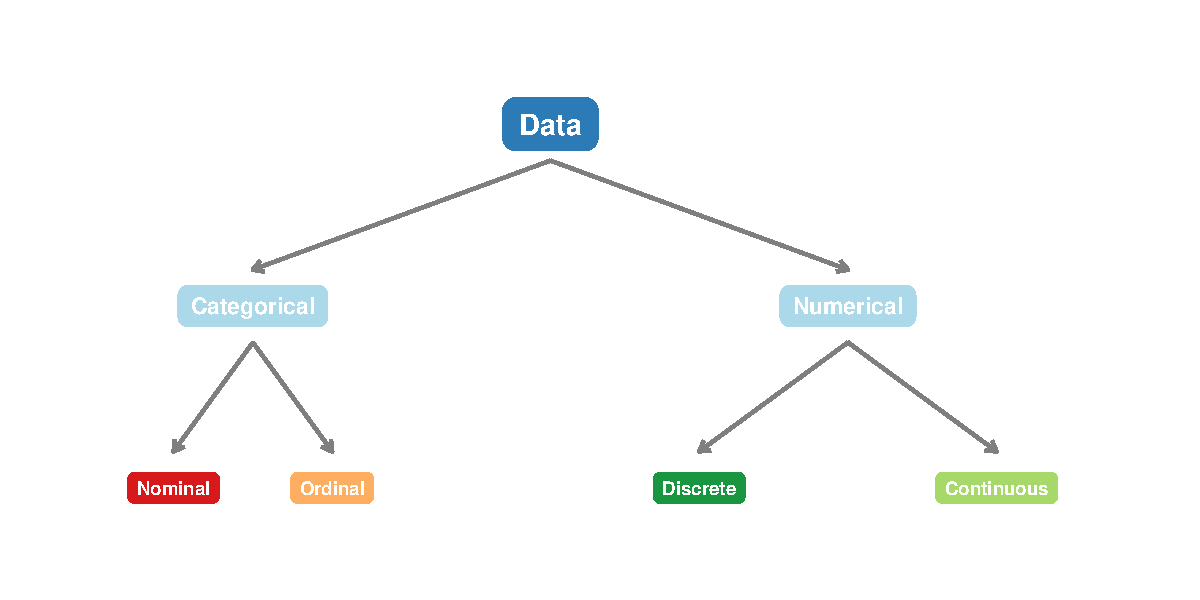
\includegraphics[keepaspectratio]{chapter01_data_in_health_science_files/figure-pdf/fig-data-types-1.pdf}}

}

\caption{\label{fig-data-types}Classification of Data Types in Health
Science}

\end{figure}%

\begin{center}\rule{0.5\linewidth}{0.5pt}\end{center}

\bookmarksetup{startatroot}

\chapter{Population and Sample}\label{population-and-sample}

\section{Population}\label{population}

A \textbf{population} is the \textbf{complete set} of all individuals or
observations that we are interested in studying.

In health research, populations are usually very large and it is
\textbf{impractical or impossible} to collect data from everyone.

\begin{quote}
\textbf{Example:} All patients with Type 2 diabetes in Thailand.
\end{quote}

\section{Sample}\label{sample}

A \textbf{sample} is a \textbf{subset} of the population that is
actually studied. We use the sample to draw conclusions (\emph{make
inferences}) about the whole population.

\begin{quote}
\textbf{Example:} 200 patients with Type 2 diabetes selected from 5
hospitals in Bangkok.
\end{quote}

\begin{tcolorbox}[enhanced jigsaw, arc=.35mm, bottomrule=.15mm, bottomtitle=1mm, breakable, colback=white, colbacktitle=quarto-callout-important-color!10!white, colframe=quarto-callout-important-color-frame, coltitle=black, left=2mm, leftrule=.75mm, opacityback=0, opacitybacktitle=0.6, rightrule=.15mm, title={⚠️ Key Principle}, titlerule=0mm, toprule=.15mm, toptitle=1mm]

A good sample must be \textbf{representative} of the population ---
meaning it should reflect the characteristics of the whole group, not
just one part of it.

\end{tcolorbox}

\begin{center}\rule{0.5\linewidth}{0.5pt}\end{center}

\section{Key Terms}\label{key-terms}

\begin{Shaded}
\begin{Highlighting}[]
\NormalTok{terms }\OtherTok{\textless{}{-}} \FunctionTok{data.frame}\NormalTok{(}
  \AttributeTok{Term =} \FunctionTok{c}\NormalTok{(}\StringTok{"Population"}\NormalTok{,}
           \StringTok{"Sample"}\NormalTok{,}
           \StringTok{"Parameter"}\NormalTok{,}
           \StringTok{"Statistic"}\NormalTok{,}
           \StringTok{"Variable"}\NormalTok{,}
           \StringTok{"Observation"}\NormalTok{),}
  \AttributeTok{Definition =} \FunctionTok{c}\NormalTok{(}
    \StringTok{"The entire group of interest"}\NormalTok{,}
    \StringTok{"A selected subset of the population"}\NormalTok{,}
    \StringTok{"A numerical summary describing the population (e.g., population mean μ)"}\NormalTok{,}
    \StringTok{"A numerical summary calculated from the sample (e.g., sample mean x̄)"}\NormalTok{,}
    \StringTok{"A characteristic being measured or observed (e.g., age, blood pressure)"}\NormalTok{,}
    \StringTok{"A single recorded value for one individual"}
\NormalTok{  ),}
  \StringTok{\textasciigrave{}}\AttributeTok{Health Example}\StringTok{\textasciigrave{}} \OtherTok{=} \FunctionTok{c}\NormalTok{(}
    \StringTok{"All nurses working in Thailand"}\NormalTok{,}
    \StringTok{"500 nurses randomly selected from 10 hospitals"}\NormalTok{,}
    \StringTok{"The true average age of ALL nurses in Thailand"}\NormalTok{,}
    \StringTok{"The average age calculated from our 500 nurses"}\NormalTok{,}
    \StringTok{"Age, gender, years of experience, ward type"}\NormalTok{,}
    \StringTok{"Nurse A: age = 28, female, 3 years experience"}
\NormalTok{  )}
\NormalTok{)}

\FunctionTok{kable}\NormalTok{(terms, }\AttributeTok{col.names =} \FunctionTok{c}\NormalTok{(}\StringTok{"Term"}\NormalTok{, }\StringTok{"Definition"}\NormalTok{, }\StringTok{"Health Science Example"}\NormalTok{),}
      \AttributeTok{align =} \FunctionTok{c}\NormalTok{(}\StringTok{"l"}\NormalTok{,}\StringTok{"l"}\NormalTok{,}\StringTok{"l"}\NormalTok{)) }\SpecialCharTok{|\textgreater{}}
  \FunctionTok{kable\_styling}\NormalTok{(}\AttributeTok{bootstrap\_options =} \FunctionTok{c}\NormalTok{(}\StringTok{"striped"}\NormalTok{,}\StringTok{"hover"}\NormalTok{,}\StringTok{"bordered"}\NormalTok{),}
                \AttributeTok{full\_width =} \ConstantTok{TRUE}\NormalTok{, }\AttributeTok{font\_size =} \DecValTok{13}\NormalTok{) }\SpecialCharTok{|\textgreater{}}
  \FunctionTok{column\_spec}\NormalTok{(}\DecValTok{1}\NormalTok{, }\AttributeTok{bold =} \ConstantTok{TRUE}\NormalTok{, }\AttributeTok{color =} \StringTok{"\#2c7bb6"}\NormalTok{)}
\end{Highlighting}
\end{Shaded}

\begin{table}

\caption{\label{tbl-terms}Important Statistical Terms}

\centering{

\begingroup\fontsize{13}{15}\selectfont

\begin{longtabu} to \linewidth {>{}l>{\raggedright}X>{\raggedright}X}
\toprule
Term & Definition & Health Science Example\\
\midrule
\textcolor[HTML]{2c7bb6}{\textbf{Population}} & The entire group of interest & All nurses working in Thailand\\
\textcolor[HTML]{2c7bb6}{\textbf{Sample}} & A selected subset of the population & 500 nurses randomly selected from 10 hospitals\\
\textcolor[HTML]{2c7bb6}{\textbf{Parameter}} & A numerical summary describing the population (e.g., population mean μ) & The true average age of ALL nurses in Thailand\\
\textcolor[HTML]{2c7bb6}{\textbf{Statistic}} & A numerical summary calculated from the sample (e.g., sample mean x̄) & |The average age calculated from our 500 nurses\\
\textcolor[HTML]{2c7bb6}{\textbf{Variable}} & A characteristic being measured or observed (e.g., age, blood pressure) & Age, gender, years of experience, ward type\\
\addlinespace
\textcolor[HTML]{2c7bb6}{\textbf{Observation}} & A single recorded value for one individual & Nurse A: age = 28, female, 3 years experience\\
\bottomrule
\end{longtabu}
\endgroup{}

}

\end{table}%

\begin{center}\rule{0.5\linewidth}{0.5pt}\end{center}

\section{Population vs.~Sample: Visual
Concept}\label{population-vs.-sample-visual-concept}

\begin{Shaded}
\begin{Highlighting}[]
\FunctionTok{set.seed}\NormalTok{(}\DecValTok{42}\NormalTok{)}
\NormalTok{n\_pop }\OtherTok{\textless{}{-}} \DecValTok{200}
\NormalTok{pop }\OtherTok{\textless{}{-}} \FunctionTok{data.frame}\NormalTok{(}
  \AttributeTok{x =} \FunctionTok{runif}\NormalTok{(n\_pop, }\DecValTok{0}\NormalTok{, }\DecValTok{10}\NormalTok{),}
  \AttributeTok{y =} \FunctionTok{runif}\NormalTok{(n\_pop, }\DecValTok{0}\NormalTok{, }\DecValTok{10}\NormalTok{),}
  \AttributeTok{group =} \StringTok{"Population"}
\NormalTok{)}

\NormalTok{sample\_idx }\OtherTok{\textless{}{-}} \FunctionTok{sample}\NormalTok{(}\DecValTok{1}\SpecialCharTok{:}\NormalTok{n\_pop, }\DecValTok{30}\NormalTok{)}
\NormalTok{pop}\SpecialCharTok{$}\NormalTok{group[sample\_idx] }\OtherTok{\textless{}{-}} \StringTok{"Sample"}

\FunctionTok{ggplot}\NormalTok{(pop, }\FunctionTok{aes}\NormalTok{(}\AttributeTok{x =}\NormalTok{ x, }\AttributeTok{y =}\NormalTok{ y, }\AttributeTok{color =}\NormalTok{ group, }\AttributeTok{size =}\NormalTok{ group, }\AttributeTok{shape =}\NormalTok{ group)) }\SpecialCharTok{+}
  \FunctionTok{geom\_point}\NormalTok{(}\AttributeTok{alpha =} \FloatTok{0.8}\NormalTok{) }\SpecialCharTok{+}
  \FunctionTok{scale\_color\_manual}\NormalTok{(}\AttributeTok{values =} \FunctionTok{c}\NormalTok{(}\StringTok{"Population"} \OtherTok{=} \StringTok{"\#b0c4de"}\NormalTok{, }\StringTok{"Sample"} \OtherTok{=} \StringTok{"\#d7191c"}\NormalTok{)) }\SpecialCharTok{+}
  \FunctionTok{scale\_size\_manual}\NormalTok{(}\AttributeTok{values =} \FunctionTok{c}\NormalTok{(}\StringTok{"Population"} \OtherTok{=} \DecValTok{2}\NormalTok{, }\StringTok{"Sample"} \OtherTok{=} \DecValTok{4}\NormalTok{)) }\SpecialCharTok{+}
  \FunctionTok{scale\_shape\_manual}\NormalTok{(}\AttributeTok{values =} \FunctionTok{c}\NormalTok{(}\StringTok{"Population"} \OtherTok{=} \DecValTok{16}\NormalTok{, }\StringTok{"Sample"} \OtherTok{=} \DecValTok{17}\NormalTok{)) }\SpecialCharTok{+}
  \FunctionTok{annotate}\NormalTok{(}\StringTok{"text"}\NormalTok{, }\AttributeTok{x =} \DecValTok{5}\NormalTok{, }\AttributeTok{y =} \FloatTok{10.5}\NormalTok{,}
           \AttributeTok{label =} \StringTok{"Population (All Patients)"}\NormalTok{,}
           \AttributeTok{size =} \FloatTok{4.5}\NormalTok{, }\AttributeTok{fontface =} \StringTok{"bold"}\NormalTok{, }\AttributeTok{color =} \StringTok{"\#2c7bb6"}\NormalTok{) }\SpecialCharTok{+}
  \FunctionTok{annotate}\NormalTok{(}\StringTok{"text"}\NormalTok{, }\AttributeTok{x =} \DecValTok{5}\NormalTok{, }\AttributeTok{y =} \SpecialCharTok{{-}}\FloatTok{0.8}\NormalTok{,}
           \AttributeTok{label =} \StringTok{"▲ Red triangles = selected sample (n = 30)"}\NormalTok{,}
           \AttributeTok{size =} \FloatTok{3.5}\NormalTok{, }\AttributeTok{color =} \StringTok{"\#d7191c"}\NormalTok{) }\SpecialCharTok{+}
  \FunctionTok{theme\_minimal}\NormalTok{(}\AttributeTok{base\_size =} \DecValTok{12}\NormalTok{) }\SpecialCharTok{+}
  \FunctionTok{theme}\NormalTok{(}\AttributeTok{legend.position =} \StringTok{"none"}\NormalTok{,}
        \AttributeTok{axis.text =} \FunctionTok{element\_blank}\NormalTok{(),}
        \AttributeTok{axis.title =} \FunctionTok{element\_blank}\NormalTok{(),}
        \AttributeTok{axis.ticks =} \FunctionTok{element\_blank}\NormalTok{(),}
        \AttributeTok{panel.grid =} \FunctionTok{element\_blank}\NormalTok{(),}
        \AttributeTok{panel.border =} \FunctionTok{element\_rect}\NormalTok{(}\AttributeTok{color =} \StringTok{"\#2c7bb6"}\NormalTok{, }\AttributeTok{fill =} \ConstantTok{NA}\NormalTok{, }\AttributeTok{linewidth =} \FloatTok{1.5}\NormalTok{)) }\SpecialCharTok{+}
  \FunctionTok{xlim}\NormalTok{(}\SpecialCharTok{{-}}\FloatTok{0.5}\NormalTok{, }\FloatTok{10.5}\NormalTok{) }\SpecialCharTok{+} \FunctionTok{ylim}\NormalTok{(}\SpecialCharTok{{-}}\FloatTok{1.2}\NormalTok{, }\DecValTok{11}\NormalTok{)}
\end{Highlighting}
\end{Shaded}

\begin{verbatim}
Warning in grid.Call.graphics(C_text, as.graphicsAnnot(x$label), x$x, x$y, :
conversion failure on '▲ Red triangles = selected sample (n = 30)' in
'mbcsToSbcs': dot substituted for <e2>
\end{verbatim}

\begin{verbatim}
Warning in grid.Call.graphics(C_text, as.graphicsAnnot(x$label), x$x, x$y, :
conversion failure on '▲ Red triangles = selected sample (n = 30)' in
'mbcsToSbcs': dot substituted for <96>
\end{verbatim}

\begin{verbatim}
Warning in grid.Call.graphics(C_text, as.graphicsAnnot(x$label), x$x, x$y, :
conversion failure on '▲ Red triangles = selected sample (n = 30)' in
'mbcsToSbcs': dot substituted for <b2>
\end{verbatim}

\begin{figure}[H]

\centering{

\pandocbounded{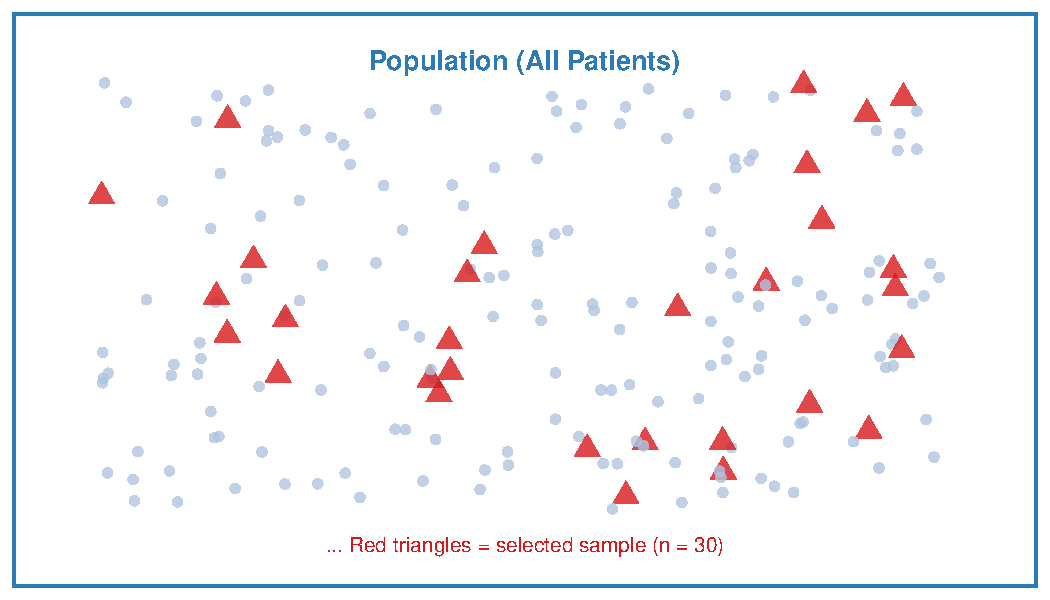
\includegraphics[keepaspectratio]{chapter01_data_in_health_science_files/figure-pdf/fig-pop-sample-1.pdf}}

}

\caption{\label{fig-pop-sample}The sample is drawn from the population
and used to make inferences}

\end{figure}%

\begin{center}\rule{0.5\linewidth}{0.5pt}\end{center}

\bookmarksetup{startatroot}

\chapter{Key Takeaways}\label{key-takeaways}

\begin{tcolorbox}[enhanced jigsaw, arc=.35mm, bottomrule=.15mm, bottomtitle=1mm, breakable, colback=white, colbacktitle=quarto-callout-note-color!10!white, colframe=quarto-callout-note-color-frame, coltitle=black, left=2mm, leftrule=.75mm, opacityback=0, opacitybacktitle=0.6, rightrule=.15mm, title={📝 Chapter 1 Summary}, titlerule=0mm, toprule=.15mm, toptitle=1mm]

\begin{enumerate}
\def\labelenumi{\arabic{enumi}.}
\item
  \textbf{Data} are recorded pieces of information collected from
  patients or research subjects.
\item
  Data are classified into two main types:

  \begin{itemize}
  \tightlist
  \item
    \textbf{Categorical}: Nominal (no order) and Ordinal (has order)
  \item
    \textbf{Numerical}: Discrete (counted, whole numbers) and Continuous
    (measured, any value)
  \end{itemize}
\item
  Identifying the \textbf{correct data type} is critical --- it
  determines which statistical methods are appropriate.
\item
  A \textbf{population} is the entire group of interest; a
  \textbf{sample} is the subset we actually study.
\item
  We use \textbf{statistics} calculated from samples to estimate
  \textbf{parameters} of the population --- this is the core idea behind
  all of biostatistics.
\end{enumerate}

\end{tcolorbox}

\begin{center}\rule{0.5\linewidth}{0.5pt}\end{center}

\bookmarksetup{startatroot}

\chapter{Examples}\label{examples}

\section{Example 1: Classify Each
Variable}\label{example-1-classify-each-variable}

A nurse researcher collects the following information from 50 patients
admitted to a medical ward:

{\def\LTcaptype{none} % do not increment counter
\begin{longtable}[]{@{}ll@{}}
\toprule\noalign{}
Variable & Recorded Values \\
\midrule\noalign{}
\endhead
\bottomrule\noalign{}
\endlastfoot
Patient ID & 001, 002, 003, \ldots{} \\
Age & 45, 62, 38, \ldots{} (years) \\
Gender & Male, Female \\
Blood type & A, B, AB, O \\
Systolic blood pressure & 118, 135, 142, \ldots{} (mmHg) \\
Pain score & 0--10 scale \\
Number of medications & 1, 2, 3, \ldots{} \\
Discharge status & Recovered, Transferred, Deceased \\
\end{longtable}
}

\begin{tcolorbox}[enhanced jigsaw, arc=.35mm, bottomrule=.15mm, bottomtitle=1mm, breakable, colback=white, colbacktitle=quarto-callout-tip-color!10!white, colframe=quarto-callout-tip-color-frame, coltitle=black, left=2mm, leftrule=.75mm, opacityback=0, opacitybacktitle=0.6, rightrule=.15mm, title={✅ Solution}, titlerule=0mm, toprule=.15mm, toptitle=1mm]

{\def\LTcaptype{none} % do not increment counter
\begin{longtable}[]{@{}
  >{\raggedright\arraybackslash}p{(\linewidth - 4\tabcolsep) * \real{0.3333}}
  >{\raggedright\arraybackslash}p{(\linewidth - 4\tabcolsep) * \real{0.3333}}
  >{\raggedright\arraybackslash}p{(\linewidth - 4\tabcolsep) * \real{0.3333}}@{}}
\toprule\noalign{}
\begin{minipage}[b]{\linewidth}\raggedright
Variable
\end{minipage} & \begin{minipage}[b]{\linewidth}\raggedright
Data Type
\end{minipage} & \begin{minipage}[b]{\linewidth}\raggedright
Reason
\end{minipage} \\
\midrule\noalign{}
\endhead
\bottomrule\noalign{}
\endlastfoot
Patient ID & --- (Identifier, not analyzed) & Just a label \\
Age & \textbf{Numerical -- Continuous} & Measured, can be 45.5 years \\
Gender & \textbf{Categorical -- Nominal} & Two categories, no order \\
Blood type & \textbf{Categorical -- Nominal} & Four categories, no
order \\
Systolic BP & \textbf{Numerical -- Continuous} & Measured in mmHg, any
value \\
Pain score & \textbf{Categorical -- Ordinal} & Has order (0 \textless{}
1 \textless{} \ldots{} \textless{} 10), but gaps unequal \\
No.~of medications & \textbf{Numerical -- Discrete} & Counted, whole
numbers only \\
Discharge status & \textbf{Categorical -- Nominal} & Three categories,
no natural order \\
\end{longtable}
}

\end{tcolorbox}

\begin{center}\rule{0.5\linewidth}{0.5pt}\end{center}

\section{Example 2: Population or
Sample?}\label{example-2-population-or-sample}

For each situation below, identify whether the group described is a
\textbf{population} or a \textbf{sample}:

\textbf{(a)} A hospital wants to know the average job satisfaction of
all 320 nurses working there. The HR department surveys all 320 nurses.

\textbf{(b)} A researcher wants to study pain levels in post-operative
patients across Thailand. She recruits 150 patients from 3 hospitals in
Chiang Mai.

\textbf{(c)} A nursing student studies the blood glucose levels of the 8
diabetic patients currently assigned to her ward.

\begin{tcolorbox}[enhanced jigsaw, arc=.35mm, bottomrule=.15mm, bottomtitle=1mm, breakable, colback=white, colbacktitle=quarto-callout-tip-color!10!white, colframe=quarto-callout-tip-color-frame, coltitle=black, left=2mm, leftrule=.75mm, opacityback=0, opacitybacktitle=0.6, rightrule=.15mm, title={✅ Solution}, titlerule=0mm, toprule=.15mm, toptitle=1mm]

\textbf{(a)} This is the \textbf{Population} --- all 320 nurses are
surveyed; no one is left out. The result is a \emph{parameter}.

\textbf{(b)} This is a \textbf{Sample} --- 150 patients from 3 hospitals
cannot represent all post-operative patients in Thailand. The result is
a \emph{statistic} used to estimate the population parameter.

\textbf{(c)} This is a \textbf{Sample} --- the 8 patients on the ward
are a small subset of all diabetic patients.

\end{tcolorbox}

\begin{center}\rule{0.5\linewidth}{0.5pt}\end{center}

\bookmarksetup{startatroot}

\chapter{Exercises}\label{exercises}

\begin{tcolorbox}[enhanced jigsaw, arc=.35mm, bottomrule=.15mm, bottomtitle=1mm, breakable, colback=white, colbacktitle=quarto-callout-caution-color!10!white, colframe=quarto-callout-caution-color-frame, coltitle=black, left=2mm, leftrule=.75mm, opacityback=0, opacitybacktitle=0.6, rightrule=.15mm, title={✏️ Exercise 1}, titlerule=0mm, toprule=.15mm, toptitle=1mm]

A public health nurse collects the following data from patients visiting
a community health clinic:

\begin{itemize}
\tightlist
\item
  Weight (kg)
\item
  Presence of hypertension (Yes / No)
\item
  Severity of hypertension (Mild / Moderate / Severe)
\item
  Number of clinic visits in the past year
\item
  Ethnicity
\item
  Body temperature (°C)
\item
  Diastolic blood pressure (mmHg)
\end{itemize}

\textbf{Classify each variable} into the correct data type and explain
your reasoning.

\end{tcolorbox}

\begin{tcolorbox}[enhanced jigsaw, arc=.35mm, bottomrule=.15mm, bottomtitle=1mm, breakable, colback=white, colbacktitle=quarto-callout-caution-color!10!white, colframe=quarto-callout-caution-color-frame, coltitle=black, left=2mm, leftrule=.75mm, opacityback=0, opacitybacktitle=0.6, rightrule=.15mm, title={✏️ Exercise 2}, titlerule=0mm, toprule=.15mm, toptitle=1mm]

A researcher is studying the prevalence of depression among elderly
patients in nursing homes across the country. She selects 200 patients
from 4 nursing homes in the central region.

\textbf{(a)} What is the population in this study?

\textbf{(b)} What is the sample?

\textbf{(c)} If the average depression score of the 200 patients is
14.2, is this number a \emph{parameter} or a \emph{statistic}? Explain.

\end{tcolorbox}

\begin{tcolorbox}[enhanced jigsaw, arc=.35mm, bottomrule=.15mm, bottomtitle=1mm, breakable, colback=white, colbacktitle=quarto-callout-caution-color!10!white, colframe=quarto-callout-caution-color-frame, coltitle=black, left=2mm, leftrule=.75mm, opacityback=0, opacitybacktitle=0.6, rightrule=.15mm, title={✏️ Exercise 3}, titlerule=0mm, toprule=.15mm, toptitle=1mm]

Look at the following list and decide whether each is an example of a
\textbf{discrete} or \textbf{continuous} variable:

\begin{enumerate}
\def\labelenumi{\arabic{enumi}.}
\tightlist
\item
  The number of patients who fell during a hospital shift
\item
  The time (in minutes) a patient waited before being seen by a doctor
\item
  The number of syringes used during a procedure
\item
  A patient's oxygen saturation level (SpO₂ \%)
\item
  The number of newborns delivered in a hospital per week
\end{enumerate}

\end{tcolorbox}

\begin{center}\rule{0.5\linewidth}{0.5pt}\end{center}

\emph{End of Chapter 1}

\begin{center}\rule{0.5\linewidth}{0.5pt}\end{center}

\begin{tcolorbox}[enhanced jigsaw, arc=.35mm, bottomrule=.15mm, bottomtitle=1mm, breakable, colback=white, colbacktitle=quarto-callout-note-color!10!white, colframe=quarto-callout-note-color-frame, coltitle=black, left=2mm, leftrule=.75mm, opacityback=0, opacitybacktitle=0.6, rightrule=.15mm, title={📚 Coming Up Next}, titlerule=0mm, toprule=.15mm, toptitle=1mm]

\textbf{Chapter 2: Data Summarization} --- How do we make sense of a
large set of patient data? We will learn to calculate means, medians,
standard deviations, and draw charts that tell a clear story.

\end{tcolorbox}

\bookmarksetup{startatroot}

\chapter{Data Summarization}\label{data-summarization}

\begin{center}\rule{0.5\linewidth}{0.5pt}\end{center}

\bookmarksetup{startatroot}

\chapter*{Introduction}\label{introduction-1}
\addcontentsline{toc}{chapter}{Introduction}

\markboth{Introduction}{Introduction}

\begin{tcolorbox}[enhanced jigsaw, arc=.35mm, bottomrule=.15mm, bottomtitle=1mm, breakable, colback=white, colbacktitle=quarto-callout-note-color!10!white, colframe=quarto-callout-note-color-frame, coltitle=black, left=2mm, leftrule=.75mm, opacityback=0, opacitybacktitle=0.6, rightrule=.15mm, title={🏥 Why Does This Matter for Nurses?}, titlerule=0mm, toprule=.15mm, toptitle=1mm]

Imagine you have blood pressure readings from 80 patients on your ward.
Looking at 80 individual numbers tells you very little. But if someone
says \emph{``the average systolic BP is 138 mmHg and most patients fall
between 120 and 155 mmHg''} --- now you have a clear picture.

\textbf{Data summarization} is the process of turning raw data into
meaningful, easy-to-understand information using numbers and charts.
This is one of the most practical skills in clinical nursing and health
research.

\end{tcolorbox}

\begin{center}\rule{0.5\linewidth}{0.5pt}\end{center}

\bookmarksetup{startatroot}

\chapter{Numerical Summarization}\label{numerical-summarization}

Numerical summarization uses \textbf{numbers} to describe the key
features of data. There are two important aspects we want to describe:

\begin{enumerate}
\def\labelenumi{\arabic{enumi}.}
\tightlist
\item
  \textbf{Central tendency} --- Where is the ``middle'' or ``typical''
  value?
\item
  \textbf{Variability} --- How spread out are the values?
\end{enumerate}

\begin{center}\rule{0.5\linewidth}{0.5pt}\end{center}

\section{Measures of Central
Tendency}\label{measures-of-central-tendency}

\subsection{Mean (Arithmetic Average)}\label{mean-arithmetic-average}

The \textbf{mean} is calculated by adding all values and dividing by the
number of observations.

\[\bar{x} = \frac{\sum_{i=1}^{n} x_i}{n} = \frac{x_1 + x_2 + \cdots + x_n}{n}\]

Where:

\begin{itemize}
\tightlist
\item
  \(\bar{x}\) = sample mean (read as ``x-bar'')
\item
  \(x_i\) = each individual value
\item
  \(n\) = total number of observations
\item
  \(\sum\) = ``sum of all''
\end{itemize}

\begin{tcolorbox}[enhanced jigsaw, arc=.35mm, bottomrule=.15mm, bottomtitle=1mm, breakable, colback=white, colbacktitle=quarto-callout-warning-color!10!white, colframe=quarto-callout-warning-color-frame, coltitle=black, left=2mm, leftrule=.75mm, opacityback=0, opacitybacktitle=0.6, rightrule=.15mm, title={⚠️ When to Use the Mean}, titlerule=0mm, toprule=.15mm, toptitle=1mm]

The mean works best for \textbf{continuous or discrete numerical data}
that is \textbf{roughly symmetric} (not heavily skewed) and has
\textbf{no extreme outliers}. A single extreme value can pull the mean
far from the typical value.

\end{tcolorbox}

\begin{center}\rule{0.5\linewidth}{0.5pt}\end{center}

\subsection{Median}\label{median}

The \textbf{median} is the \textbf{middle value} when all observations
are arranged in order.

\begin{itemize}
\tightlist
\item
  If \(n\) is \textbf{odd}: the median is the value at position
  \(\dfrac{n+1}{2}\)
\item
  If \(n\) is \textbf{even}: the median is the \textbf{average of the
  two middle values} at positions \(\dfrac{n}{2}\) and
  \(\dfrac{n}{2}+1\)
\end{itemize}

\begin{tcolorbox}[enhanced jigsaw, arc=.35mm, bottomrule=.15mm, bottomtitle=1mm, breakable, colback=white, colbacktitle=quarto-callout-warning-color!10!white, colframe=quarto-callout-warning-color-frame, coltitle=black, left=2mm, leftrule=.75mm, opacityback=0, opacitybacktitle=0.6, rightrule=.15mm, title={⚠️ When to Use the Median}, titlerule=0mm, toprule=.15mm, toptitle=1mm]

The median is preferred when data is \textbf{skewed} or has
\textbf{outliers}, because it is not affected by extreme values. It is
also the appropriate measure for \textbf{ordinal data}.

\end{tcolorbox}

\begin{center}\rule{0.5\linewidth}{0.5pt}\end{center}

\subsection{Mode}\label{mode}

The \textbf{mode} is the value that appears \textbf{most frequently} in
the data.

\begin{itemize}
\tightlist
\item
  A dataset can have \textbf{one mode} (unimodal), \textbf{two modes}
  (bimodal), or \textbf{no mode} (all values appear equally).
\item
  The mode is the only measure of central tendency appropriate for
  \textbf{nominal data}.
\end{itemize}

\begin{center}\rule{0.5\linewidth}{0.5pt}\end{center}

\subsection{Choosing the Right
Measure}\label{choosing-the-right-measure}

\begin{Shaded}
\begin{Highlighting}[]
\NormalTok{ct }\OtherTok{\textless{}{-}} \FunctionTok{data.frame}\NormalTok{(}
  \AttributeTok{Measure =} \FunctionTok{c}\NormalTok{(}\StringTok{"Mean"}\NormalTok{, }\StringTok{"Median"}\NormalTok{, }\StringTok{"Mode"}\NormalTok{),}
  \StringTok{\textasciigrave{}}\AttributeTok{Best For}\StringTok{\textasciigrave{}} \OtherTok{=} \FunctionTok{c}\NormalTok{(}
    \StringTok{"Numerical data (continuous or discrete), symmetric distribution"}\NormalTok{,}
    \StringTok{"Numerical data with skewness or outliers; Ordinal data"}\NormalTok{,}
    \StringTok{"Nominal data; finding the most common category"}
\NormalTok{  ),}
  \StringTok{\textasciigrave{}}\AttributeTok{Nursing Example}\StringTok{\textasciigrave{}} \OtherTok{=} \FunctionTok{c}\NormalTok{(}
    \StringTok{"Average patient age, average blood glucose"}\NormalTok{,}
    \StringTok{"Average length of hospital stay (skewed by long{-}stay patients)"}\NormalTok{,}
    \StringTok{"Most common blood type on a ward, most frequent pain score"}
\NormalTok{  )}
\NormalTok{)}

\FunctionTok{kable}\NormalTok{(ct, }\AttributeTok{col.names =} \FunctionTok{c}\NormalTok{(}\StringTok{"Measure"}\NormalTok{, }\StringTok{"Best For"}\NormalTok{, }\StringTok{"Nursing Example"}\NormalTok{),}
      \AttributeTok{align =} \FunctionTok{c}\NormalTok{(}\StringTok{"l"}\NormalTok{,}\StringTok{"l"}\NormalTok{,}\StringTok{"l"}\NormalTok{)) }\SpecialCharTok{|\textgreater{}}
  \FunctionTok{kable\_styling}\NormalTok{(}\AttributeTok{bootstrap\_options =} \FunctionTok{c}\NormalTok{(}\StringTok{"striped"}\NormalTok{,}\StringTok{"hover"}\NormalTok{,}\StringTok{"bordered"}\NormalTok{),}
                \AttributeTok{full\_width =} \ConstantTok{TRUE}\NormalTok{, }\AttributeTok{font\_size =} \DecValTok{13}\NormalTok{) }\SpecialCharTok{|\textgreater{}}
  \FunctionTok{column\_spec}\NormalTok{(}\DecValTok{1}\NormalTok{, }\AttributeTok{bold =} \ConstantTok{TRUE}\NormalTok{, }\AttributeTok{color =} \StringTok{"\#2c7bb6"}\NormalTok{)}
\end{Highlighting}
\end{Shaded}

\begin{table}

\caption{\label{tbl-central}Choosing the Right Measure of Central
Tendency}

\centering{

\begingroup\fontsize{13}{15}\selectfont

\begin{longtabu} to \linewidth {>{}l>{\raggedright}X>{\raggedright}X}
\toprule
Measure & Best For & Nursing Example\\
\midrule
\textcolor[HTML]{2c7bb6}{\textbf{Mean}} & Numerical data (continuous or discrete), symmetric distribution & Average patient age, average blood glucose\\
\textcolor[HTML]{2c7bb6}{\textbf{Median}} & Numerical data with skewness or outliers; Ordinal data & Average length of hospital stay (skewed by long-stay patients)\\
\textcolor[HTML]{2c7bb6}{\textbf{Mode}} & Nominal data; finding the most common category & Most common blood type on a ward, most frequent pain score\\
\bottomrule
\end{longtabu}
\endgroup{}

}

\end{table}%

\begin{center}\rule{0.5\linewidth}{0.5pt}\end{center}

\section{Measures of Variability}\label{measures-of-variability}

Knowing the average alone is not enough. Two wards might have the same
average patient age but very different spreads --- one ward may have all
patients aged 55--65, another may have patients aged 20--90. Variability
tells us how \textbf{spread out} the data are.

\subsection{Range}\label{range}

The \textbf{range} is the simplest measure of spread:

\[\text{Range} = \text{Maximum value} - \text{Minimum value}\]

\begin{tcolorbox}[enhanced jigsaw, arc=.35mm, bottomrule=.15mm, bottomtitle=1mm, breakable, colback=white, colbacktitle=quarto-callout-warning-color!10!white, colframe=quarto-callout-warning-color-frame, coltitle=black, left=2mm, leftrule=.75mm, opacityback=0, opacitybacktitle=0.6, rightrule=.15mm, title={⚠️ Limitation}, titlerule=0mm, toprule=.15mm, toptitle=1mm]

The range only uses two values (max and min) and is very sensitive to
outliers.

\end{tcolorbox}

\begin{center}\rule{0.5\linewidth}{0.5pt}\end{center}

\subsection{Variance}\label{variance}

The \textbf{variance} measures the average squared distance of each
value from the mean.

\textbf{Population variance:}
\[\sigma^2 = \frac{\sum_{i=1}^{N}(x_i - \mu)^2}{N}\]

\textbf{Sample variance} (used more often in practice):
\[s^2 = \frac{\sum_{i=1}^{n}(x_i - \bar{x})^2}{n-1}\]

Where:

\begin{itemize}
\tightlist
\item
  \(\mu\) = population mean, \(\bar{x}\) = sample mean
\item
  \(N\) = population size, \(n\) = sample size
\item
  \(n-1\) in the denominator corrects for the fact that we're using a
  sample
\end{itemize}

\begin{center}\rule{0.5\linewidth}{0.5pt}\end{center}

\subsection{Standard Deviation}\label{standard-deviation}

The \textbf{standard deviation (SD)} is the square root of the variance.
It is expressed in the \textbf{same units as the original data}, making
it much easier to interpret than variance.

\[s = \sqrt{s^2} = \sqrt{\frac{\sum_{i=1}^{n}(x_i - \bar{x})^2}{n-1}}\]

\begin{tcolorbox}[enhanced jigsaw, arc=.35mm, bottomrule=.15mm, bottomtitle=1mm, breakable, colback=white, colbacktitle=quarto-callout-tip-color!10!white, colframe=quarto-callout-tip-color-frame, coltitle=black, left=2mm, leftrule=.75mm, opacityback=0, opacitybacktitle=0.6, rightrule=.15mm, title={💡 Interpreting Standard Deviation}, titlerule=0mm, toprule=.15mm, toptitle=1mm]

A \textbf{small SD} means values are clustered closely around the mean.
A \textbf{large SD} means values are widely spread.

In clinical practice, you may see lab reports written as: \textbf{Mean ±
SD}, for example: Hemoglobin = \textbf{12.5 ± 1.8 g/dL}

\end{tcolorbox}

\begin{center}\rule{0.5\linewidth}{0.5pt}\end{center}

\subsection{Summary: Numerical
Measures}\label{summary-numerical-measures}

\begin{Shaded}
\begin{Highlighting}[]
\NormalTok{vm }\OtherTok{\textless{}{-}} \FunctionTok{data.frame}\NormalTok{(}
  \AttributeTok{Measure =} \FunctionTok{c}\NormalTok{(}\StringTok{"Mean"}\NormalTok{, }\StringTok{"Median"}\NormalTok{, }\StringTok{"Mode"}\NormalTok{, }\StringTok{"Range"}\NormalTok{, }\StringTok{"Variance"}\NormalTok{, }\StringTok{"Standard Deviation"}\NormalTok{),}
  \AttributeTok{Symbol =} \FunctionTok{c}\NormalTok{(}\StringTok{"$}\SpecialCharTok{\textbackslash{}\textbackslash{}}\StringTok{bar\{x\}$"}\NormalTok{, }\StringTok{"Md"}\NormalTok{, }\StringTok{"Mo"}\NormalTok{, }\StringTok{"Max − Min"}\NormalTok{, }\StringTok{"$s\^{}2$"}\NormalTok{, }\StringTok{"$s$"}\NormalTok{),}
  \AttributeTok{Purpose =} \FunctionTok{c}\NormalTok{(}\StringTok{"Central tendency"}\NormalTok{, }\StringTok{"Central tendency"}\NormalTok{,}
               \StringTok{"Central tendency"}\NormalTok{, }\StringTok{"Spread"}\NormalTok{,}
               \StringTok{"Spread (squared units)"}\NormalTok{, }\StringTok{"Spread (original units)"}\NormalTok{),}
  \StringTok{\textasciigrave{}}\AttributeTok{Data Type}\StringTok{\textasciigrave{}} \OtherTok{=} \FunctionTok{c}\NormalTok{(}\StringTok{"Numerical"}\NormalTok{, }\StringTok{"Numerical / Ordinal"}\NormalTok{,}
                   \StringTok{"Any"}\NormalTok{, }\StringTok{"Numerical"}\NormalTok{,}
                   \StringTok{"Numerical"}\NormalTok{, }\StringTok{"Numerical"}\NormalTok{)}
\NormalTok{)}

\FunctionTok{kable}\NormalTok{(vm, }\AttributeTok{col.names =} \FunctionTok{c}\NormalTok{(}\StringTok{"Measure"}\NormalTok{,}\StringTok{"Symbol"}\NormalTok{,}\StringTok{"Purpose"}\NormalTok{,}\StringTok{"Appropriate Data Type"}\NormalTok{),}
      \AttributeTok{align =} \FunctionTok{c}\NormalTok{(}\StringTok{"l"}\NormalTok{,}\StringTok{"c"}\NormalTok{,}\StringTok{"l"}\NormalTok{,}\StringTok{"l"}\NormalTok{), }\AttributeTok{escape =} \ConstantTok{FALSE}\NormalTok{) }\SpecialCharTok{|\textgreater{}}
  \FunctionTok{kable\_styling}\NormalTok{(}\AttributeTok{bootstrap\_options =} \FunctionTok{c}\NormalTok{(}\StringTok{"striped"}\NormalTok{,}\StringTok{"hover"}\NormalTok{,}\StringTok{"bordered"}\NormalTok{),}
                \AttributeTok{full\_width =} \ConstantTok{TRUE}\NormalTok{, }\AttributeTok{font\_size =} \DecValTok{13}\NormalTok{) }\SpecialCharTok{|\textgreater{}}
  \FunctionTok{column\_spec}\NormalTok{(}\DecValTok{1}\NormalTok{, }\AttributeTok{bold =} \ConstantTok{TRUE}\NormalTok{, }\AttributeTok{color =} \StringTok{"\#2c7bb6"}\NormalTok{)}
\end{Highlighting}
\end{Shaded}

\begin{table}

\caption{\label{tbl-variability}Summary of Numerical Summary Measures}

\centering{

\begingroup\fontsize{13}{15}\selectfont

\begin{longtabu} to \linewidth {>{}l>{\centering}X>{\raggedright}X>{\raggedright}X}
\toprule
Measure & Symbol & Purpose & Appropriate Data Type\\
\midrule
\textcolor[HTML]{2c7bb6}{\textbf{Mean}} & \$\textbackslash{}bar\{x\}\$ & Central tendency & Numerical\\
\textcolor[HTML]{2c7bb6}{\textbf{Median}} & Md & Central tendency & Numerical / Ordinal\\
\textcolor[HTML]{2c7bb6}{\textbf{Mode}} & Mo & Central tendency & Any\\
\textcolor[HTML]{2c7bb6}{\textbf{Range}} & Max − Min & Spread & Numerical\\
\textcolor[HTML]{2c7bb6}{\textbf{Variance}} & \$s\textasciicircum{}2\$ & Spread (squared units) & Numerical\\
\addlinespace
\textcolor[HTML]{2c7bb6}{\textbf{Standard Deviation}} & \$s\$ & Spread (original units) & Numerical\\
\bottomrule
\end{longtabu}
\endgroup{}

}

\end{table}%

\begin{center}\rule{0.5\linewidth}{0.5pt}\end{center}

\bookmarksetup{startatroot}

\chapter{Pictorial Summarization}\label{pictorial-summarization}

Charts and graphs turn numbers into visual stories. The correct chart
depends on the \textbf{data type}.

\section{Bar Chart}\label{bar-chart}

Used for \textbf{categorical data} (nominal or ordinal). Each bar
represents a category; the height shows the count or percentage.

\begin{Shaded}
\begin{Highlighting}[]
\NormalTok{blood }\OtherTok{\textless{}{-}} \FunctionTok{data.frame}\NormalTok{(}
  \AttributeTok{type =} \FunctionTok{c}\NormalTok{(}\StringTok{"A"}\NormalTok{, }\StringTok{"B"}\NormalTok{, }\StringTok{"AB"}\NormalTok{, }\StringTok{"O"}\NormalTok{),}
  \AttributeTok{count =} \FunctionTok{c}\NormalTok{(}\DecValTok{38}\NormalTok{, }\DecValTok{27}\NormalTok{, }\DecValTok{15}\NormalTok{, }\DecValTok{40}\NormalTok{)}
\NormalTok{)}

\FunctionTok{ggplot}\NormalTok{(blood, }\FunctionTok{aes}\NormalTok{(}\AttributeTok{x =}\NormalTok{ type, }\AttributeTok{y =}\NormalTok{ count, }\AttributeTok{fill =}\NormalTok{ type)) }\SpecialCharTok{+}
  \FunctionTok{geom\_bar}\NormalTok{(}\AttributeTok{stat =} \StringTok{"identity"}\NormalTok{, }\AttributeTok{width =} \FloatTok{0.6}\NormalTok{, }\AttributeTok{color =} \StringTok{"white"}\NormalTok{) }\SpecialCharTok{+}
  \FunctionTok{geom\_text}\NormalTok{(}\FunctionTok{aes}\NormalTok{(}\AttributeTok{label =}\NormalTok{ count), }\AttributeTok{vjust =} \SpecialCharTok{{-}}\FloatTok{0.5}\NormalTok{, }\AttributeTok{size =} \FloatTok{4.5}\NormalTok{, }\AttributeTok{fontface =} \StringTok{"bold"}\NormalTok{) }\SpecialCharTok{+}
  \FunctionTok{scale\_fill\_manual}\NormalTok{(}\AttributeTok{values =} \FunctionTok{c}\NormalTok{(}\StringTok{"\#2c7bb6"}\NormalTok{,}\StringTok{"\#abd9e9"}\NormalTok{,}\StringTok{"\#d7191c"}\NormalTok{,}\StringTok{"\#fdae61"}\NormalTok{)) }\SpecialCharTok{+}
  \FunctionTok{labs}\NormalTok{(}\AttributeTok{x =} \StringTok{"Blood Type"}\NormalTok{, }\AttributeTok{y =} \StringTok{"Number of Patients"}\NormalTok{) }\SpecialCharTok{+}
  \FunctionTok{theme\_minimal}\NormalTok{(}\AttributeTok{base\_size =} \DecValTok{13}\NormalTok{) }\SpecialCharTok{+}
  \FunctionTok{theme}\NormalTok{(}\AttributeTok{legend.position =} \StringTok{"none"}\NormalTok{,}
        \AttributeTok{panel.grid.major.x =} \FunctionTok{element\_blank}\NormalTok{())}
\end{Highlighting}
\end{Shaded}

\begin{figure}[H]

\centering{

\pandocbounded{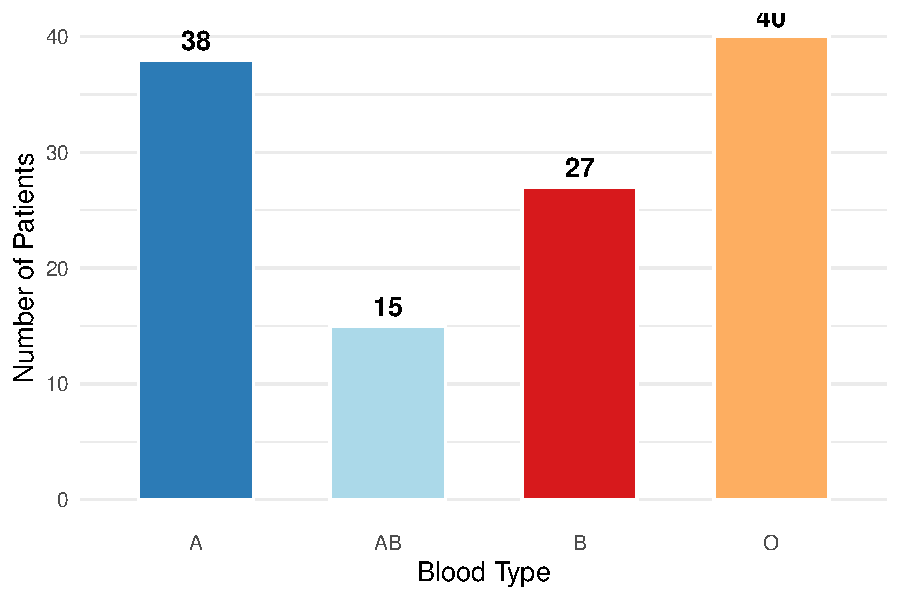
\includegraphics[keepaspectratio]{chapter02_data_summarization_files/figure-pdf/fig-bar-1.pdf}}

}

\caption{\label{fig-bar}Bar Chart: Blood Types of 120 Patients in a
Medical Ward}

\end{figure}%

\begin{center}\rule{0.5\linewidth}{0.5pt}\end{center}

\section{Histogram}\label{histogram}

Used for \textbf{continuous numerical data}. Bars are drawn over class
intervals (ranges of values); bars touch each other because the data is
continuous.

\begin{Shaded}
\begin{Highlighting}[]
\FunctionTok{set.seed}\NormalTok{(}\DecValTok{123}\NormalTok{)}
\NormalTok{bp\_data }\OtherTok{\textless{}{-}} \FunctionTok{data.frame}\NormalTok{(}\AttributeTok{sbp =} \FunctionTok{round}\NormalTok{(}\FunctionTok{rnorm}\NormalTok{(}\DecValTok{80}\NormalTok{, }\AttributeTok{mean =} \DecValTok{130}\NormalTok{, }\AttributeTok{sd =} \DecValTok{15}\NormalTok{)))}

\FunctionTok{ggplot}\NormalTok{(bp\_data, }\FunctionTok{aes}\NormalTok{(}\AttributeTok{x =}\NormalTok{ sbp)) }\SpecialCharTok{+}
  \FunctionTok{geom\_histogram}\NormalTok{(}\AttributeTok{binwidth =} \DecValTok{10}\NormalTok{, }\AttributeTok{fill =} \StringTok{"\#2c7bb6"}\NormalTok{, }\AttributeTok{color =} \StringTok{"white"}\NormalTok{, }\AttributeTok{alpha =} \FloatTok{0.85}\NormalTok{) }\SpecialCharTok{+}
  \FunctionTok{labs}\NormalTok{(}\AttributeTok{x =} \StringTok{"Systolic Blood Pressure (mmHg)"}\NormalTok{, }\AttributeTok{y =} \StringTok{"Number of Patients"}\NormalTok{) }\SpecialCharTok{+}
  \FunctionTok{theme\_minimal}\NormalTok{(}\AttributeTok{base\_size =} \DecValTok{13}\NormalTok{) }\SpecialCharTok{+}
  \FunctionTok{theme}\NormalTok{(}\AttributeTok{panel.grid.minor =} \FunctionTok{element\_blank}\NormalTok{())}
\end{Highlighting}
\end{Shaded}

\begin{figure}[H]

\centering{

\pandocbounded{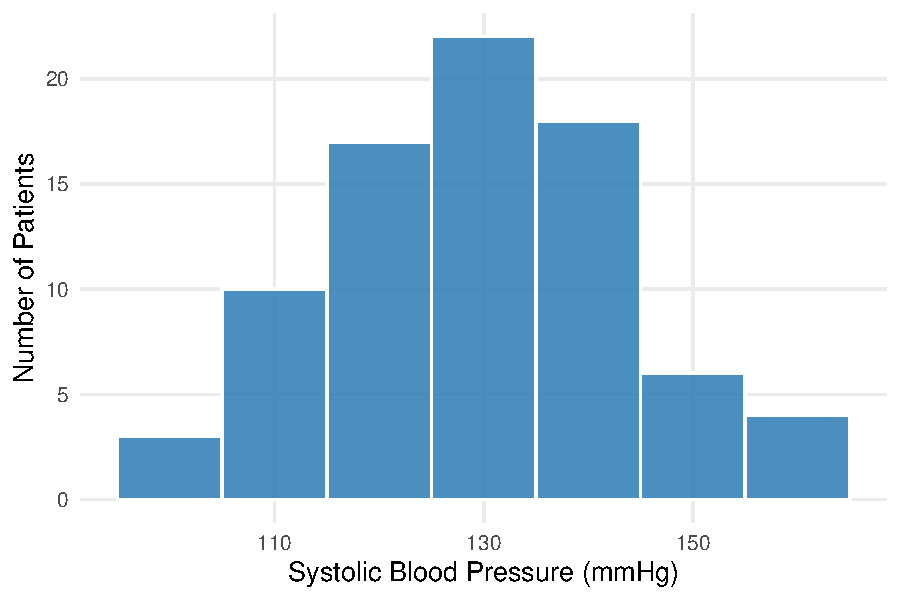
\includegraphics[keepaspectratio]{chapter02_data_summarization_files/figure-pdf/fig-hist-1.pdf}}

}

\caption{\label{fig-hist}Histogram: Systolic Blood Pressure of 80
Patients}

\end{figure}%

\begin{tcolorbox}[enhanced jigsaw, arc=.35mm, bottomrule=.15mm, bottomtitle=1mm, breakable, colback=white, colbacktitle=quarto-callout-tip-color!10!white, colframe=quarto-callout-tip-color-frame, coltitle=black, left=2mm, leftrule=.75mm, opacityback=0, opacitybacktitle=0.6, rightrule=.15mm, title={💡 Bar Chart vs Histogram}, titlerule=0mm, toprule=.15mm, toptitle=1mm]

{\def\LTcaptype{none} % do not increment counter
\begin{longtable}[]{@{}lll@{}}
\toprule\noalign{}
& Bar Chart & Histogram \\
\midrule\noalign{}
\endhead
\bottomrule\noalign{}
\endlastfoot
Data type & Categorical & Continuous numerical \\
Bars & Separated (gaps) & Touching (no gaps) \\
X-axis & Categories & Numerical ranges \\
\end{longtable}
}

\end{tcolorbox}

\begin{center}\rule{0.5\linewidth}{0.5pt}\end{center}

\section{Box Plot (Box-and-Whisker
Plot)}\label{box-plot-box-and-whisker-plot}

A \textbf{box plot} summarizes the \textbf{distribution} of numerical
data using 5 key values (the \textbf{five-number summary}):

{\def\LTcaptype{none} % do not increment counter
\begin{longtable}[]{@{}ll@{}}
\toprule\noalign{}
Value & Description \\
\midrule\noalign{}
\endhead
\bottomrule\noalign{}
\endlastfoot
Minimum & Smallest value (excluding outliers) \\
Q1 & 25th percentile (lower quartile) \\
Median (Q2) & 50th percentile --- middle value \\
Q3 & 75th percentile (upper quartile) \\
Maximum & Largest value (excluding outliers) \\
\end{longtable}
}

The \textbf{Interquartile Range (IQR) = Q3 − Q1} represents the middle
50\% of data. Points beyond \textbf{1.5 × IQR} from Q1 or Q3 are marked
as \textbf{outliers (○)}.

\begin{Shaded}
\begin{Highlighting}[]
\FunctionTok{set.seed}\NormalTok{(}\DecValTok{99}\NormalTok{)}
\NormalTok{stay }\OtherTok{\textless{}{-}} \FunctionTok{data.frame}\NormalTok{(}
  \AttributeTok{days =} \FunctionTok{c}\NormalTok{(}\FunctionTok{rexp}\NormalTok{(}\DecValTok{50}\NormalTok{, }\FloatTok{0.3}\NormalTok{), }\FunctionTok{rexp}\NormalTok{(}\DecValTok{50}\NormalTok{, }\FloatTok{0.5}\NormalTok{)),}
  \AttributeTok{ward =} \FunctionTok{rep}\NormalTok{(}\FunctionTok{c}\NormalTok{(}\StringTok{"Medical Ward"}\NormalTok{, }\StringTok{"Surgical Ward"}\NormalTok{), }\AttributeTok{each =} \DecValTok{50}\NormalTok{)}
\NormalTok{)}

\FunctionTok{ggplot}\NormalTok{(stay, }\FunctionTok{aes}\NormalTok{(}\AttributeTok{x =}\NormalTok{ ward, }\AttributeTok{y =}\NormalTok{ days, }\AttributeTok{fill =}\NormalTok{ ward)) }\SpecialCharTok{+}
  \FunctionTok{geom\_boxplot}\NormalTok{(}\AttributeTok{width =} \FloatTok{0.5}\NormalTok{, }\AttributeTok{outlier.color =} \StringTok{"\#d7191c"}\NormalTok{,}
               \AttributeTok{outlier.shape =} \DecValTok{1}\NormalTok{, }\AttributeTok{outlier.size =} \DecValTok{3}\NormalTok{, }\AttributeTok{alpha =} \FloatTok{0.8}\NormalTok{) }\SpecialCharTok{+}
  \FunctionTok{scale\_fill\_manual}\NormalTok{(}\AttributeTok{values =} \FunctionTok{c}\NormalTok{(}\StringTok{"\#abd9e9"}\NormalTok{,}\StringTok{"\#fdae61"}\NormalTok{)) }\SpecialCharTok{+}
  \FunctionTok{labs}\NormalTok{(}\AttributeTok{x =} \StringTok{""}\NormalTok{, }\AttributeTok{y =} \StringTok{"Length of Stay (days)"}\NormalTok{) }\SpecialCharTok{+}
  \FunctionTok{theme\_minimal}\NormalTok{(}\AttributeTok{base\_size =} \DecValTok{13}\NormalTok{) }\SpecialCharTok{+}
  \FunctionTok{theme}\NormalTok{(}\AttributeTok{legend.position =} \StringTok{"none"}\NormalTok{,}
        \AttributeTok{panel.grid.major.x =} \FunctionTok{element\_blank}\NormalTok{())}
\end{Highlighting}
\end{Shaded}

\begin{figure}[H]

\centering{

\pandocbounded{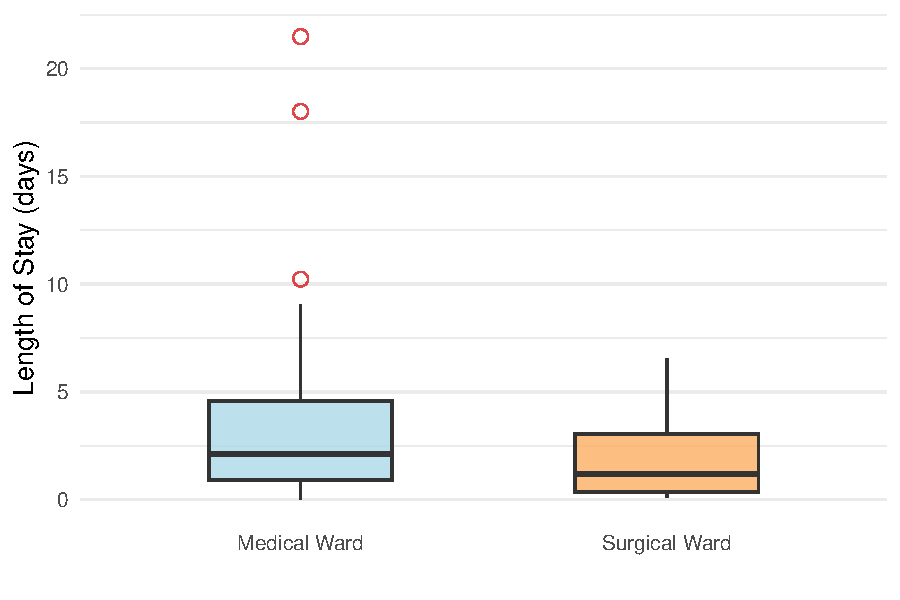
\includegraphics[keepaspectratio]{chapter02_data_summarization_files/figure-pdf/fig-boxplot-1.pdf}}

}

\caption{\label{fig-boxplot}Box Plot: Comparing Length of Hospital Stay
Between Two Wards}

\end{figure}%

\begin{center}\rule{0.5\linewidth}{0.5pt}\end{center}

\section{Choosing the Right Chart}\label{choosing-the-right-chart}

\begin{Shaded}
\begin{Highlighting}[]
\NormalTok{charts }\OtherTok{\textless{}{-}} \FunctionTok{data.frame}\NormalTok{(}
  \StringTok{\textasciigrave{}}\AttributeTok{Chart Type}\StringTok{\textasciigrave{}} \OtherTok{=} \FunctionTok{c}\NormalTok{(}\StringTok{"Bar Chart"}\NormalTok{, }\StringTok{"Pie Chart"}\NormalTok{, }\StringTok{"Histogram"}\NormalTok{, }\StringTok{"Box Plot"}\NormalTok{),}
  \StringTok{\textasciigrave{}}\AttributeTok{Data Type}\StringTok{\textasciigrave{}} \OtherTok{=} \FunctionTok{c}\NormalTok{(}\StringTok{"Categorical (Nominal/Ordinal)"}\NormalTok{,}
                   \StringTok{"Categorical (Nominal) — proportions"}\NormalTok{,}
                   \StringTok{"Numerical (Continuous)"}\NormalTok{,}
                   \StringTok{"Numerical (Continuous/Discrete)"}\NormalTok{),}
  \StringTok{\textasciigrave{}}\AttributeTok{What It Shows}\StringTok{\textasciigrave{}} \OtherTok{=} \FunctionTok{c}\NormalTok{(}
    \StringTok{"Frequency or percentage of each category"}\NormalTok{,}
    \StringTok{"Proportion of each category as a slice of the whole"}\NormalTok{,}
    \StringTok{"Distribution shape, spread, and central tendency"}\NormalTok{,}
    \StringTok{"Median, spread, quartiles, and outliers"}
\NormalTok{  ),}
  \StringTok{\textasciigrave{}}\AttributeTok{Nursing Example}\StringTok{\textasciigrave{}} \OtherTok{=} \FunctionTok{c}\NormalTok{(}
    \StringTok{"Number of patients by blood type"}\NormalTok{,}
    \StringTok{"Proportion of patients by diagnosis"}\NormalTok{,}
    \StringTok{"Distribution of patient ages or blood pressure"}\NormalTok{,}
    \StringTok{"Comparing recovery time between two wards"}
\NormalTok{  )}
\NormalTok{)}

\FunctionTok{kable}\NormalTok{(charts,}
      \AttributeTok{col.names =} \FunctionTok{c}\NormalTok{(}\StringTok{"Chart Type"}\NormalTok{,}\StringTok{"Data Type"}\NormalTok{,}\StringTok{"What It Shows"}\NormalTok{,}\StringTok{"Nursing Example"}\NormalTok{),}
      \AttributeTok{align =} \FunctionTok{c}\NormalTok{(}\StringTok{"l"}\NormalTok{,}\StringTok{"l"}\NormalTok{,}\StringTok{"l"}\NormalTok{,}\StringTok{"l"}\NormalTok{)) }\SpecialCharTok{|\textgreater{}}
  \FunctionTok{kable\_styling}\NormalTok{(}\AttributeTok{bootstrap\_options =} \FunctionTok{c}\NormalTok{(}\StringTok{"striped"}\NormalTok{,}\StringTok{"hover"}\NormalTok{,}\StringTok{"bordered"}\NormalTok{),}
                \AttributeTok{full\_width =} \ConstantTok{TRUE}\NormalTok{, }\AttributeTok{font\_size =} \DecValTok{13}\NormalTok{) }\SpecialCharTok{|\textgreater{}}
  \FunctionTok{column\_spec}\NormalTok{(}\DecValTok{1}\NormalTok{, }\AttributeTok{bold =} \ConstantTok{TRUE}\NormalTok{, }\AttributeTok{color =} \StringTok{"\#2c7bb6"}\NormalTok{)}
\end{Highlighting}
\end{Shaded}

\begin{table}

\caption{\label{tbl-charts}Guide to Choosing the Right Chart}

\centering{

\begingroup\fontsize{13}{15}\selectfont

\begin{longtabu} to \linewidth {>{}l>{\raggedright}X>{\raggedright}X>{\raggedright}X}
\toprule
Chart Type & Data Type & What It Shows & Nursing Example\\
\midrule
\textcolor[HTML]{2c7bb6}{\textbf{Bar Chart}} & Categorical (Nominal/Ordinal) & Frequency or percentage of each category & Number of patients by blood type\\
\textcolor[HTML]{2c7bb6}{\textbf{Pie Chart}} & Categorical (Nominal) — proportions & Proportion of each category as a slice of the whole & Proportion of patients by diagnosis\\
\textcolor[HTML]{2c7bb6}{\textbf{Histogram}} & Numerical (Continuous) & Distribution shape, spread, and central tendency & Distribution of patient ages or blood pressure\\
\textcolor[HTML]{2c7bb6}{\textbf{Box Plot}} & Numerical (Continuous/Discrete) & Median, spread, quartiles, and outliers & Comparing recovery time between two wards\\
\bottomrule
\end{longtabu}
\endgroup{}

}

\end{table}%

\begin{center}\rule{0.5\linewidth}{0.5pt}\end{center}

\bookmarksetup{startatroot}

\chapter{Key Takeaways}\label{key-takeaways-1}

\begin{tcolorbox}[enhanced jigsaw, arc=.35mm, bottomrule=.15mm, bottomtitle=1mm, breakable, colback=white, colbacktitle=quarto-callout-note-color!10!white, colframe=quarto-callout-note-color-frame, coltitle=black, left=2mm, leftrule=.75mm, opacityback=0, opacitybacktitle=0.6, rightrule=.15mm, title={📝 Chapter 2 Summary}, titlerule=0mm, toprule=.15mm, toptitle=1mm]

\begin{enumerate}
\def\labelenumi{\arabic{enumi}.}
\item
  \textbf{Numerical summarization} uses measures of \emph{central
  tendency} (mean, median, mode) and \emph{variability} (range,
  variance, SD) to describe data with numbers.
\item
  The \textbf{mean} is best for symmetric numerical data; the
  \textbf{median} is better when data is skewed or has outliers; the
  \textbf{mode} is used for categorical data.
\item
  The \textbf{standard deviation (SD)} is the most commonly reported
  measure of spread in clinical research, expressed in the same units as
  the data.
\item
  \textbf{Pictorial summarization} uses charts: bar charts for
  categorical data, histograms for continuous data, and box plots to
  compare groups and identify outliers.
\item
  Always choose the \textbf{correct summary measure and chart} based on
  the \textbf{data type} --- using the wrong one leads to misleading
  conclusions.
\end{enumerate}

\end{tcolorbox}

\begin{center}\rule{0.5\linewidth}{0.5pt}\end{center}

\bookmarksetup{startatroot}

\chapter{Examples}\label{examples-1}

\section{Example 1: Calculating Mean, Median, and
SD}\label{example-1-calculating-mean-median-and-sd}

A nurse records the resting heart rate (beats per minute) of \textbf{9
patients}:

\[72, \; 68, \; 85, \; 74, \; 90, \; 68, \; 78, \; 72, \; 110\]

Calculate the \textbf{(a) mean}, \textbf{(b) median}, and \textbf{(c)
standard deviation}.

\begin{tcolorbox}[enhanced jigsaw, arc=.35mm, bottomrule=.15mm, bottomtitle=1mm, breakable, colback=white, colbacktitle=quarto-callout-tip-color!10!white, colframe=quarto-callout-tip-color-frame, coltitle=black, left=2mm, leftrule=.75mm, opacityback=0, opacitybacktitle=0.6, rightrule=.15mm, title={✅ Solution}, titlerule=0mm, toprule=.15mm, toptitle=1mm]

\textbf{Step 1 --- Arrange data in order:}

\[68, \; 68, \; 72, \; 72, \; 74, \; 78, \; 85, \; 90, \; 110\]

\begin{center}\rule{0.5\linewidth}{0.5pt}\end{center}

\textbf{(a) Mean:}

\[\bar{x} = \frac{68+68+72+72+74+78+85+90+110}{9} = \frac{717}{9} = 79.7 \text{ bpm}\]

\begin{center}\rule{0.5\linewidth}{0.5pt}\end{center}

\textbf{(b) Median:}

\(n = 9\) (odd), so median is at position \(\dfrac{9+1}{2} = 5\)th
value.

Counting from the ordered list: the 5th value = \textbf{74 bpm}

Notice that the median (74) is lower than the mean (79.7) because the
outlier value of 110 pulls the mean upward.

\begin{center}\rule{0.5\linewidth}{0.5pt}\end{center}

\textbf{(c) Standard Deviation:}

First, find each \((x_i - \bar{x})^2\):

\begin{Shaded}
\begin{Highlighting}[]
\NormalTok{hr }\OtherTok{\textless{}{-}} \FunctionTok{c}\NormalTok{(}\DecValTok{68}\NormalTok{, }\DecValTok{68}\NormalTok{, }\DecValTok{72}\NormalTok{, }\DecValTok{72}\NormalTok{, }\DecValTok{74}\NormalTok{, }\DecValTok{78}\NormalTok{, }\DecValTok{85}\NormalTok{, }\DecValTok{90}\NormalTok{, }\DecValTok{110}\NormalTok{)}
\NormalTok{xbar }\OtherTok{\textless{}{-}} \FunctionTok{mean}\NormalTok{(hr)}

\NormalTok{sd\_table }\OtherTok{\textless{}{-}} \FunctionTok{data.frame}\NormalTok{(}
  \StringTok{\textasciigrave{}}\AttributeTok{Patient}\StringTok{\textasciigrave{}} \OtherTok{=} \FunctionTok{paste0}\NormalTok{(}\StringTok{"Patient "}\NormalTok{, }\DecValTok{1}\SpecialCharTok{:}\DecValTok{9}\NormalTok{),}
  \StringTok{\textasciigrave{}}\AttributeTok{Heart Rate (xᵢ)}\StringTok{\textasciigrave{}} \OtherTok{=}\NormalTok{ hr,}
  \StringTok{\textasciigrave{}}\AttributeTok{xᵢ − x̄}\StringTok{\textasciigrave{}} \OtherTok{=} \FunctionTok{round}\NormalTok{(hr }\SpecialCharTok{{-}}\NormalTok{ xbar, }\DecValTok{1}\NormalTok{),}
  \StringTok{\textasciigrave{}}\AttributeTok{(xᵢ − x̄)²}\StringTok{\textasciigrave{}} \OtherTok{=} \FunctionTok{round}\NormalTok{((hr }\SpecialCharTok{{-}}\NormalTok{ xbar)}\SpecialCharTok{\^{}}\DecValTok{2}\NormalTok{, }\DecValTok{2}\NormalTok{)}
\NormalTok{)}

\FunctionTok{kable}\NormalTok{(sd\_table,}
      \AttributeTok{col.names =} \FunctionTok{c}\NormalTok{(}\StringTok{"Patient"}\NormalTok{, }\StringTok{"Heart Rate (xᵢ)"}\NormalTok{, }\StringTok{"xᵢ − x̄"}\NormalTok{, }\StringTok{"(xᵢ − x̄)²"}\NormalTok{),}
      \AttributeTok{align =} \FunctionTok{c}\NormalTok{(}\StringTok{"l"}\NormalTok{,}\StringTok{"c"}\NormalTok{,}\StringTok{"c"}\NormalTok{,}\StringTok{"c"}\NormalTok{)) }\SpecialCharTok{|\textgreater{}}
  \FunctionTok{kable\_styling}\NormalTok{(}\AttributeTok{bootstrap\_options =} \FunctionTok{c}\NormalTok{(}\StringTok{"striped"}\NormalTok{,}\StringTok{"hover"}\NormalTok{,}\StringTok{"bordered"}\NormalTok{),}
                \AttributeTok{full\_width =} \ConstantTok{FALSE}\NormalTok{, }\AttributeTok{font\_size =} \DecValTok{13}\NormalTok{) }\SpecialCharTok{|\textgreater{}}
  \FunctionTok{row\_spec}\NormalTok{(}\DecValTok{9}\NormalTok{, }\AttributeTok{bold =} \ConstantTok{TRUE}\NormalTok{) }\SpecialCharTok{|\textgreater{}}
  \FunctionTok{row\_spec}\NormalTok{(}\DecValTok{0}\NormalTok{, }\AttributeTok{bold =} \ConstantTok{TRUE}\NormalTok{, }\AttributeTok{color =} \StringTok{"white"}\NormalTok{, }\AttributeTok{background =} \StringTok{"\#2c7bb6"}\NormalTok{)}
\end{Highlighting}
\end{Shaded}

\begingroup\fontsize{13}{15}\selectfont

\begin{longtable}[t]{lccc}

\caption{\label{tbl-sd-calc}Step-by-step SD calculation}

\tabularnewline

\toprule
\cellcolor[HTML]{2c7bb6}{\textcolor{white}{\textbf{Patient}}} & \cellcolor[HTML]{2c7bb6}{\textcolor{white}{\textbf{Heart Rate (xᵢ)}}} & \cellcolor[HTML]{2c7bb6}{\textcolor{white}{\textbf{xᵢ − x̄}}} & \cellcolor[HTML]{2c7bb6}{\textcolor{white}{\textbf{| (xᵢ − x̄)}}}\\
\midrule
Patient 1 & 68 & -11.7 & 136.11\\
Patient 2 & 68 & -11.7 & 136.11\\
Patient 3 & 72 & -7.7 & 58.78\\
Patient 4 & 72 & -7.7 & 58.78\\
Patient 5 & 74 & -5.7 & 32.11\\
\addlinespace
Patient 6 & 78 & -1.7 & 2.78\\
Patient 7 & 85 & 5.3 & 28.44\\
Patient 8 & 90 & 10.3 & 106.78\\
\textbf{Patient 9} & \textbf{110} & \textbf{30.3} & \textbf{920.11}\\
\bottomrule

\end{longtable}

\endgroup{}

\[\sum(x_i - \bar{x})^2 = 1480\]

\[s^2 = \frac{1480}{9-1} = \frac{1480}{8} = 185\]

\[s = \sqrt{185} = 13.6 \text{ bpm}\]

\textbf{Interpretation:} The average heart rate is \textbf{79.7 ± 13.5
bpm}. The relatively large SD reflects the wide spread, largely
influenced by the patient with 110 bpm.

\end{tcolorbox}

\begin{center}\rule{0.5\linewidth}{0.5pt}\end{center}

\section{Example 2: Choosing the Right Summary and
Chart}\label{example-2-choosing-the-right-summary-and-chart}

A hospital administrator records the \textbf{diagnosis} of 200 patients
admitted last month and wants to summarize the data. A research nurse
records the \textbf{length of stay (days)} for the same 200 patients.

\begin{tcolorbox}[enhanced jigsaw, arc=.35mm, bottomrule=.15mm, bottomtitle=1mm, breakable, colback=white, colbacktitle=quarto-callout-tip-color!10!white, colframe=quarto-callout-tip-color-frame, coltitle=black, left=2mm, leftrule=.75mm, opacityback=0, opacitybacktitle=0.6, rightrule=.15mm, title={✅ Solution}, titlerule=0mm, toprule=.15mm, toptitle=1mm]

{\def\LTcaptype{none} % do not increment counter
\begin{longtable}[]{@{}
  >{\raggedright\arraybackslash}p{(\linewidth - 6\tabcolsep) * \real{0.2500}}
  >{\raggedright\arraybackslash}p{(\linewidth - 6\tabcolsep) * \real{0.2500}}
  >{\raggedright\arraybackslash}p{(\linewidth - 6\tabcolsep) * \real{0.2500}}
  >{\raggedright\arraybackslash}p{(\linewidth - 6\tabcolsep) * \real{0.2500}}@{}}
\toprule\noalign{}
\begin{minipage}[b]{\linewidth}\raggedright
Variable
\end{minipage} & \begin{minipage}[b]{\linewidth}\raggedright
Data Type
\end{minipage} & \begin{minipage}[b]{\linewidth}\raggedright
Best Summary Measure
\end{minipage} & \begin{minipage}[b]{\linewidth}\raggedright
Best Chart
\end{minipage} \\
\midrule\noalign{}
\endhead
\bottomrule\noalign{}
\endlastfoot
Diagnosis & Categorical -- Nominal & Mode (most common diagnosis) & Bar
Chart \\
Length of stay & Numerical -- Continuous (likely skewed) & Median + IQR
& Box Plot or Histogram \\
\end{longtable}
}

\textbf{Why median for length of stay?} Hospital stays are almost always
right-skewed --- most patients stay a few days, but a small number may
stay for weeks or months. These long-stay patients would pull the mean
upward, making it misleading. The median better represents the
``typical'' patient.

\end{tcolorbox}

\begin{center}\rule{0.5\linewidth}{0.5pt}\end{center}

\bookmarksetup{startatroot}

\chapter{Exercises}\label{exercises-1}

\begin{tcolorbox}[enhanced jigsaw, arc=.35mm, bottomrule=.15mm, bottomtitle=1mm, breakable, colback=white, colbacktitle=quarto-callout-caution-color!10!white, colframe=quarto-callout-caution-color-frame, coltitle=black, left=2mm, leftrule=.75mm, opacityback=0, opacitybacktitle=0.6, rightrule=.15mm, title={✏️ Exercise 1}, titlerule=0mm, toprule=.15mm, toptitle=1mm]

A nurse records the body temperature (°C) of \textbf{10 patients} at
8:00 AM:

\[37.2, \; 36.8, \; 38.5, \; 37.0, \; 39.1, \; 36.8, \; 37.5, \; 38.0, \; 37.2, \; 40.2\]

\textbf{(a)} Calculate the \textbf{mean} body temperature.

\textbf{(b)} Find the \textbf{median} body temperature.

\textbf{(c)} What is the \textbf{mode}?

\textbf{(d)} Calculate the \textbf{range}.

\textbf{(e)} Calculate the \textbf{standard deviation}. Show all steps.

\textbf{(f)} One patient has a temperature of 40.2°C. How does this
value affect the mean compared to the median? Which measure would you
report to the physician, and why?

\end{tcolorbox}

\begin{tcolorbox}[enhanced jigsaw, arc=.35mm, bottomrule=.15mm, bottomtitle=1mm, breakable, colback=white, colbacktitle=quarto-callout-caution-color!10!white, colframe=quarto-callout-caution-color-frame, coltitle=black, left=2mm, leftrule=.75mm, opacityback=0, opacitybacktitle=0.6, rightrule=.15mm, title={✏️ Exercise 2}, titlerule=0mm, toprule=.15mm, toptitle=1mm]

A community health nurse surveys \textbf{50 elderly patients} and
records:

\begin{itemize}
\tightlist
\item
  \textbf{Gender} (Male / Female)
\item
  \textbf{Systolic blood pressure} (mmHg)
\item
  \textbf{Self-rated health} (Poor / Fair / Good / Very Good /
  Excellent)
\end{itemize}

For each variable, state:

\textbf{(a)} The data type.

\textbf{(b)} The most appropriate measure of central tendency.

\textbf{(c)} The most appropriate chart to display the data.

\end{tcolorbox}

\begin{tcolorbox}[enhanced jigsaw, arc=.35mm, bottomrule=.15mm, bottomtitle=1mm, breakable, colback=white, colbacktitle=quarto-callout-caution-color!10!white, colframe=quarto-callout-caution-color-frame, coltitle=black, left=2mm, leftrule=.75mm, opacityback=0, opacitybacktitle=0.6, rightrule=.15mm, title={✏️ Exercise 3}, titlerule=0mm, toprule=.15mm, toptitle=1mm]

The number of patient falls recorded each month over \textbf{12 months}
in a hospital ward are:

\[2, \; 0, \; 3, \; 1, \; 4, \; 2, \; 1, \; 0, \; 3, \; 2, \; 5, \; 1\]

\textbf{(a)} Calculate the mean and median number of falls per month.

\textbf{(b)} Draw a \textbf{bar chart} (by hand or describe what it
would look like) showing the frequency of each number of falls.

\textbf{(c)} The ward manager wants to set a monthly target. Should she
use the mean or median as the baseline? Explain.

\end{tcolorbox}

\begin{center}\rule{0.5\linewidth}{0.5pt}\end{center}

\emph{End of Chapter 2}

\begin{center}\rule{0.5\linewidth}{0.5pt}\end{center}

\begin{tcolorbox}[enhanced jigsaw, arc=.35mm, bottomrule=.15mm, bottomtitle=1mm, breakable, colback=white, colbacktitle=quarto-callout-note-color!10!white, colframe=quarto-callout-note-color-frame, coltitle=black, left=2mm, leftrule=.75mm, opacityback=0, opacitybacktitle=0.6, rightrule=.15mm, title={📚 Coming Up Next}, titlerule=0mm, toprule=.15mm, toptitle=1mm]

\textbf{Chapter 3: Random Variable and Probability Distribution} --- We
will learn what a random variable is, how probabilities work, and why
the \textbf{normal distribution} (bell curve) is so important in health
science research.

\end{tcolorbox}

\bookmarksetup{startatroot}

\chapter{Random Variable and Probability
Distribution}\label{random-variable-and-probability-distribution}

\begin{center}\rule{0.5\linewidth}{0.5pt}\end{center}

\bookmarksetup{startatroot}

\chapter*{Introduction}\label{introduction-2}
\addcontentsline{toc}{chapter}{Introduction}

\markboth{Introduction}{Introduction}

\begin{tcolorbox}[enhanced jigsaw, arc=.35mm, bottomrule=.15mm, bottomtitle=1mm, breakable, colback=white, colbacktitle=quarto-callout-note-color!10!white, colframe=quarto-callout-note-color-frame, coltitle=black, left=2mm, leftrule=.75mm, opacityback=0, opacitybacktitle=0.6, rightrule=.15mm, title={💡 Why Does This Matter?}, titlerule=0mm, toprule=.15mm, toptitle=1mm]

When we collect data --- patient ages, blood pressure readings, test
results --- we rarely get the same value twice. Outcomes vary, and that
variation follows patterns we can describe mathematically.

Understanding \textbf{how data is distributed} allows us to answer
questions like:

\begin{itemize}
\tightlist
\item
  What is the probability that a randomly selected patient has a fever
  above 39°C?
\item
  What proportion of adults have a BMI in the healthy range?
\item
  How unusual is a blood pressure reading of 160 mmHg in this
  population?
\end{itemize}

In this chapter, we introduce the concepts of \textbf{frequency
distributions} and the \textbf{normal distribution} --- the most
important probability distribution in all of biostatistics.

\end{tcolorbox}

\begin{center}\rule{0.5\linewidth}{0.5pt}\end{center}

\bookmarksetup{startatroot}

\chapter{Frequency Distributions}\label{frequency-distributions}

\section{What Is a Frequency
Distribution?}\label{what-is-a-frequency-distribution}

A \textbf{frequency distribution} is a systematic way of organizing raw
data into a table that shows how often each value (or range of values)
occurs.

It answers the simple question: \emph{``How many times does each value
appear?''}

\begin{center}\rule{0.5\linewidth}{0.5pt}\end{center}

\section{Frequency Distribution for Categorical
Data}\label{frequency-distribution-for-categorical-data}

For categorical variables, we simply count how many observations fall
into each category.

\begin{tcolorbox}[enhanced jigsaw, arc=.35mm, bottomrule=.15mm, bottomtitle=1mm, breakable, colback=white, colbacktitle=quarto-callout-tip-color!10!white, colframe=quarto-callout-tip-color-frame, coltitle=black, left=2mm, leftrule=.75mm, opacityback=0, opacitybacktitle=0.6, rightrule=.15mm, title={📋 Example}, titlerule=0mm, toprule=.15mm, toptitle=1mm]

Blood types of 200 patients admitted to a hospital last month:

\begin{Shaded}
\begin{Highlighting}[]
\NormalTok{blood }\OtherTok{\textless{}{-}} \FunctionTok{data.frame}\NormalTok{(}
  \StringTok{\textasciigrave{}}\AttributeTok{Blood Type}\StringTok{\textasciigrave{}} \OtherTok{=} \FunctionTok{c}\NormalTok{(}\StringTok{"A"}\NormalTok{, }\StringTok{"B"}\NormalTok{, }\StringTok{"AB"}\NormalTok{, }\StringTok{"O"}\NormalTok{, }\StringTok{"**Total**"}\NormalTok{),}
  \AttributeTok{Frequency =} \FunctionTok{c}\NormalTok{(}\DecValTok{76}\NormalTok{, }\DecValTok{54}\NormalTok{, }\DecValTok{30}\NormalTok{, }\DecValTok{40}\NormalTok{, }\DecValTok{200}\NormalTok{),}
  \StringTok{\textasciigrave{}}\AttributeTok{Relative Frequency}\StringTok{\textasciigrave{}} \OtherTok{=} \FunctionTok{c}\NormalTok{(}\StringTok{"76/200 = 0.38"}\NormalTok{, }\StringTok{"54/200 = 0.27"}\NormalTok{,}
                             \StringTok{"30/200 = 0.15"}\NormalTok{, }\StringTok{"40/200 = 0.20"}\NormalTok{,}
                             \StringTok{"200/200 = **1.00**"}\NormalTok{),}
  \AttributeTok{Percentage =} \FunctionTok{c}\NormalTok{(}\StringTok{"38\%"}\NormalTok{, }\StringTok{"27\%"}\NormalTok{, }\StringTok{"15\%"}\NormalTok{, }\StringTok{"20\%"}\NormalTok{, }\StringTok{"**100\%**"}\NormalTok{)}
\NormalTok{)}

\FunctionTok{kable}\NormalTok{(blood,}
      \AttributeTok{col.names =} \FunctionTok{c}\NormalTok{(}\StringTok{"Blood Type"}\NormalTok{, }\StringTok{"Frequency (f)"}\NormalTok{,}
                    \StringTok{"Relative Frequency (f/n)"}\NormalTok{, }\StringTok{"Percentage"}\NormalTok{),}
      \AttributeTok{align =} \FunctionTok{c}\NormalTok{(}\StringTok{"c"}\NormalTok{,}\StringTok{"c"}\NormalTok{,}\StringTok{"c"}\NormalTok{,}\StringTok{"c"}\NormalTok{), }\AttributeTok{escape =} \ConstantTok{FALSE}\NormalTok{) }\SpecialCharTok{|\textgreater{}}
  \FunctionTok{kable\_styling}\NormalTok{(}\AttributeTok{bootstrap\_options =} \FunctionTok{c}\NormalTok{(}\StringTok{"striped"}\NormalTok{,}\StringTok{"hover"}\NormalTok{,}\StringTok{"bordered"}\NormalTok{),}
                \AttributeTok{full\_width =} \ConstantTok{FALSE}\NormalTok{, }\AttributeTok{font\_size =} \DecValTok{13}\NormalTok{) }\SpecialCharTok{|\textgreater{}}
  \FunctionTok{row\_spec}\NormalTok{(}\DecValTok{5}\NormalTok{, }\AttributeTok{bold =} \ConstantTok{TRUE}\NormalTok{, }\AttributeTok{background =} \StringTok{"\#f0f0f0"}\NormalTok{) }\SpecialCharTok{|\textgreater{}}
  \FunctionTok{column\_spec}\NormalTok{(}\DecValTok{1}\NormalTok{, }\AttributeTok{bold =} \ConstantTok{TRUE}\NormalTok{)}
\end{Highlighting}
\end{Shaded}

\begingroup\fontsize{13}{15}\selectfont

\begin{longtable}[t]{>{}cccc}

\caption{\label{tbl-cat-freq}Frequency Distribution: Blood Type of 200
Patients}

\tabularnewline

\toprule
Blood Type & Frequency (f) & Relative Frequency (f/n) & Percentage\\
\midrule
\textbf{A} & 76 & 76/200 = 0.38 & 38\%\\
\textbf{B} & 54 & 54/200 = 0.27 & 27\%\\
\textbf{AB} & 30 & 30/200 = 0.15 & 15\%\\
\textbf{O} & 40 & 40/200 = 0.20 & 20\%\\
\textbf{\cellcolor[HTML]{f0f0f0}{\textbf{**Total**}}} & \cellcolor[HTML]{f0f0f0}{\textbf{200}} & \cellcolor[HTML]{f0f0f0}{\textbf{200/200 = **1.00**}} & \cellcolor[HTML]{f0f0f0}{\textbf{**100\%**}}\\
\bottomrule

\end{longtable}

\endgroup{}

\end{tcolorbox}

\textbf{Relative frequency} = \(\dfrac{f}{n}\), where \(f\) is the count
for that category and \(n\) is the total number of observations.

\begin{center}\rule{0.5\linewidth}{0.5pt}\end{center}

\section{Frequency Distribution for Continuous
Data}\label{frequency-distribution-for-continuous-data}

For continuous variables, we group values into \textbf{class intervals}
(also called \emph{bins}) and count how many observations fall in each
interval.

\textbf{Steps to construct a frequency distribution table:}

\begin{enumerate}
\def\labelenumi{\arabic{enumi}.}
\tightlist
\item
  Find the \textbf{range} = Maximum − Minimum
\item
  Choose the \textbf{number of classes} (typically 5--10)
\item
  Calculate \textbf{class width} =
  \(\dfrac{\text{Range}}{\text{Number of classes}}\) (round up)
\item
  List the class intervals and count observations in each
\end{enumerate}

\begin{tcolorbox}[enhanced jigsaw, arc=.35mm, bottomrule=.15mm, bottomtitle=1mm, breakable, colback=white, colbacktitle=quarto-callout-tip-color!10!white, colframe=quarto-callout-tip-color-frame, coltitle=black, left=2mm, leftrule=.75mm, opacityback=0, opacitybacktitle=0.6, rightrule=.15mm, title={📋 Example}, titlerule=0mm, toprule=.15mm, toptitle=1mm]

Systolic blood pressure (mmHg) of 80 patients:

\begin{Shaded}
\begin{Highlighting}[]
\FunctionTok{set.seed}\NormalTok{(}\DecValTok{123}\NormalTok{)}
\NormalTok{sbp }\OtherTok{\textless{}{-}} \FunctionTok{round}\NormalTok{(}\FunctionTok{rnorm}\NormalTok{(}\DecValTok{80}\NormalTok{, }\AttributeTok{mean =} \DecValTok{130}\NormalTok{, }\AttributeTok{sd =} \DecValTok{15}\NormalTok{))}

\NormalTok{breaks }\OtherTok{\textless{}{-}} \FunctionTok{seq}\NormalTok{(}\DecValTok{95}\NormalTok{, }\DecValTok{175}\NormalTok{, }\AttributeTok{by =} \DecValTok{10}\NormalTok{)}
\NormalTok{labels }\OtherTok{\textless{}{-}} \FunctionTok{paste0}\NormalTok{(breaks[}\SpecialCharTok{{-}}\FunctionTok{length}\NormalTok{(breaks)], }\StringTok{"–"}\NormalTok{, breaks[}\SpecialCharTok{{-}}\DecValTok{1}\NormalTok{] }\SpecialCharTok{{-}} \DecValTok{1}\NormalTok{)}
\NormalTok{sbp\_cut }\OtherTok{\textless{}{-}} \FunctionTok{cut}\NormalTok{(sbp, }\AttributeTok{breaks =}\NormalTok{ breaks, }\AttributeTok{right =} \ConstantTok{FALSE}\NormalTok{, }\AttributeTok{labels =}\NormalTok{ labels)}
\NormalTok{freq\_table }\OtherTok{\textless{}{-}} \FunctionTok{as.data.frame}\NormalTok{(}\FunctionTok{table}\NormalTok{(sbp\_cut))}
\FunctionTok{colnames}\NormalTok{(freq\_table) }\OtherTok{\textless{}{-}} \FunctionTok{c}\NormalTok{(}\StringTok{"Class Interval (mmHg)"}\NormalTok{, }\StringTok{"Frequency (f)"}\NormalTok{)}
\NormalTok{freq\_table}\SpecialCharTok{$}\StringTok{\textasciigrave{}}\AttributeTok{Relative Frequency}\StringTok{\textasciigrave{}} \OtherTok{\textless{}{-}} \FunctionTok{round}\NormalTok{(freq\_table}\SpecialCharTok{$}\StringTok{\textasciigrave{}}\AttributeTok{Frequency (f)}\StringTok{\textasciigrave{}} \SpecialCharTok{/} \DecValTok{80}\NormalTok{, }\DecValTok{3}\NormalTok{)}
\NormalTok{freq\_table}\SpecialCharTok{$}\StringTok{\textasciigrave{}}\AttributeTok{Cumulative Frequency}\StringTok{\textasciigrave{}} \OtherTok{\textless{}{-}} \FunctionTok{cumsum}\NormalTok{(freq\_table}\SpecialCharTok{$}\StringTok{\textasciigrave{}}\AttributeTok{Frequency (f)}\StringTok{\textasciigrave{}}\NormalTok{)}

\FunctionTok{kable}\NormalTok{(freq\_table, }\AttributeTok{align =} \FunctionTok{c}\NormalTok{(}\StringTok{"c"}\NormalTok{,}\StringTok{"c"}\NormalTok{,}\StringTok{"c"}\NormalTok{,}\StringTok{"c"}\NormalTok{)) }\SpecialCharTok{|\textgreater{}}
  \FunctionTok{kable\_styling}\NormalTok{(}\AttributeTok{bootstrap\_options =} \FunctionTok{c}\NormalTok{(}\StringTok{"striped"}\NormalTok{,}\StringTok{"hover"}\NormalTok{,}\StringTok{"bordered"}\NormalTok{),}
                \AttributeTok{full\_width =} \ConstantTok{FALSE}\NormalTok{, }\AttributeTok{font\_size =} \DecValTok{13}\NormalTok{) }\SpecialCharTok{|\textgreater{}}
  \FunctionTok{column\_spec}\NormalTok{(}\DecValTok{1}\NormalTok{, }\AttributeTok{bold =} \ConstantTok{TRUE}\NormalTok{)}
\end{Highlighting}
\end{Shaded}

\begingroup\fontsize{13}{15}\selectfont

\begin{longtable}[t]{>{}cccc}

\caption{\label{tbl-cont-freq}Frequency Distribution: Systolic Blood
Pressure of 80 Patients}

\tabularnewline

\toprule
Class Interval (mmHg) & Frequency (f) & Relative Frequency & Cumulative Frequency\\
\midrule
\textbf{95–104} & 2 & 0.025 & 2\\
\textbf{105–114} & 9 & 0.112 & 11\\
\textbf{115–124} & 17 & 0.212 & 28\\
\textbf{125–134} & 22 & 0.275 & 50\\
\textbf{135–144} & 18 & 0.225 & 68\\
\addlinespace
\textbf{145–154} & 8 & 0.100 & 76\\
\textbf{155–164} & 4 & 0.050 & 80\\
\textbf{165–174} & 0 & 0.000 & 80\\
\bottomrule

\end{longtable}

\endgroup{}

\end{tcolorbox}

\textbf{Cumulative frequency} tells us how many observations fall
\emph{at or below} the upper boundary of each class --- useful for
answering questions like \emph{``What proportion of patients have SBP
below 140 mmHg?''}

\begin{center}\rule{0.5\linewidth}{0.5pt}\end{center}

\section{Visualizing Frequency
Distributions}\label{visualizing-frequency-distributions}

A frequency distribution table can be visualized as a
\textbf{histogram}, where the height of each bar represents the
frequency of that class interval.

\begin{Shaded}
\begin{Highlighting}[]
\FunctionTok{set.seed}\NormalTok{(}\DecValTok{123}\NormalTok{)}
\NormalTok{sbp\_data }\OtherTok{\textless{}{-}} \FunctionTok{data.frame}\NormalTok{(}\AttributeTok{sbp =} \FunctionTok{round}\NormalTok{(}\FunctionTok{rnorm}\NormalTok{(}\DecValTok{80}\NormalTok{, }\AttributeTok{mean =} \DecValTok{130}\NormalTok{, }\AttributeTok{sd =} \DecValTok{15}\NormalTok{)))}

\FunctionTok{ggplot}\NormalTok{(sbp\_data, }\FunctionTok{aes}\NormalTok{(}\AttributeTok{x =}\NormalTok{ sbp)) }\SpecialCharTok{+}
  \FunctionTok{geom\_histogram}\NormalTok{(}\AttributeTok{breaks =} \FunctionTok{seq}\NormalTok{(}\DecValTok{95}\NormalTok{, }\DecValTok{175}\NormalTok{, }\AttributeTok{by =} \DecValTok{10}\NormalTok{),}
                 \AttributeTok{fill =} \StringTok{"\#2c7bb6"}\NormalTok{, }\AttributeTok{color =} \StringTok{"white"}\NormalTok{, }\AttributeTok{alpha =} \FloatTok{0.85}\NormalTok{) }\SpecialCharTok{+}
  \FunctionTok{labs}\NormalTok{(}\AttributeTok{x =} \StringTok{"Systolic Blood Pressure (mmHg)"}\NormalTok{, }\AttributeTok{y =} \StringTok{"Frequency"}\NormalTok{) }\SpecialCharTok{+}
  \FunctionTok{scale\_x\_continuous}\NormalTok{(}\AttributeTok{breaks =} \FunctionTok{seq}\NormalTok{(}\DecValTok{95}\NormalTok{, }\DecValTok{175}\NormalTok{, }\AttributeTok{by =} \DecValTok{10}\NormalTok{)) }\SpecialCharTok{+}
  \FunctionTok{theme\_minimal}\NormalTok{(}\AttributeTok{base\_size =} \DecValTok{13}\NormalTok{) }\SpecialCharTok{+}
  \FunctionTok{theme}\NormalTok{(}\AttributeTok{panel.grid.minor =} \FunctionTok{element\_blank}\NormalTok{())}
\end{Highlighting}
\end{Shaded}

\begin{figure}[H]

\centering{

\pandocbounded{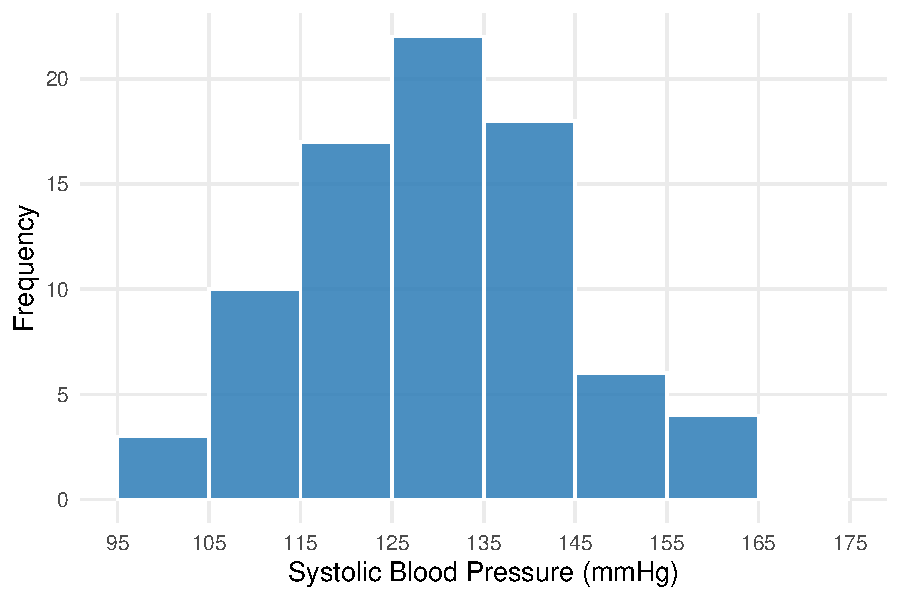
\includegraphics[keepaspectratio]{chapter03_probability_distribution_files/figure-pdf/fig-hist-freq-1.pdf}}

}

\caption{\label{fig-hist-freq}Histogram of Systolic Blood Pressure (80
patients)}

\end{figure}%

The \textbf{shape} of the histogram is important --- it tells us about
the \textbf{distribution} of the data, which leads us to the next
section.

\begin{center}\rule{0.5\linewidth}{0.5pt}\end{center}

\bookmarksetup{startatroot}

\chapter{The Normal Distribution}\label{the-normal-distribution}

\section{What Is the Normal
Distribution?}\label{what-is-the-normal-distribution}

The \textbf{normal distribution} (also called the \emph{Gaussian
distribution} or \emph{bell curve}) is the most important probability
distribution in statistics.

Many biological and clinical measurements naturally follow --- or
approximately follow --- a normal distribution:

\begin{itemize}
\tightlist
\item
  Adult height and body weight
\item
  Blood pressure in a healthy population
\item
  Serum cholesterol levels
\item
  Birth weight of newborns
\end{itemize}

\begin{Shaded}
\begin{Highlighting}[]
\NormalTok{x }\OtherTok{\textless{}{-}} \FunctionTok{seq}\NormalTok{(}\SpecialCharTok{{-}}\DecValTok{4}\NormalTok{, }\DecValTok{4}\NormalTok{, }\AttributeTok{length =} \DecValTok{500}\NormalTok{)}
\NormalTok{y }\OtherTok{\textless{}{-}} \FunctionTok{dnorm}\NormalTok{(x)}
\NormalTok{df }\OtherTok{\textless{}{-}} \FunctionTok{data.frame}\NormalTok{(}\AttributeTok{x =}\NormalTok{ x, }\AttributeTok{y =}\NormalTok{ y)}

\FunctionTok{ggplot}\NormalTok{(df, }\FunctionTok{aes}\NormalTok{(x, y)) }\SpecialCharTok{+}
  \FunctionTok{geom\_line}\NormalTok{(}\AttributeTok{color =} \StringTok{"\#2c7bb6"}\NormalTok{, }\AttributeTok{linewidth =} \FloatTok{1.4}\NormalTok{) }\SpecialCharTok{+}
  \FunctionTok{geom\_area}\NormalTok{(}\AttributeTok{fill =} \StringTok{"\#abd9e9"}\NormalTok{, }\AttributeTok{alpha =} \FloatTok{0.4}\NormalTok{) }\SpecialCharTok{+}
  \FunctionTok{geom\_vline}\NormalTok{(}\AttributeTok{xintercept =} \DecValTok{0}\NormalTok{, }\AttributeTok{linetype =} \StringTok{"dashed"}\NormalTok{, }\AttributeTok{color =} \StringTok{"\#d7191c"}\NormalTok{, }\AttributeTok{linewidth =} \DecValTok{1}\NormalTok{) }\SpecialCharTok{+}
  \FunctionTok{annotate}\NormalTok{(}\StringTok{"text"}\NormalTok{, }\AttributeTok{x =} \DecValTok{0}\NormalTok{, }\AttributeTok{y =} \FloatTok{0.43}\NormalTok{, }\AttributeTok{label =} \StringTok{"Mean = Median = Mode"}\NormalTok{,}
           \AttributeTok{color =} \StringTok{"\#d7191c"}\NormalTok{, }\AttributeTok{size =} \DecValTok{4}\NormalTok{, }\AttributeTok{hjust =} \FloatTok{0.5}\NormalTok{) }\SpecialCharTok{+}
  \FunctionTok{scale\_x\_continuous}\NormalTok{(}\AttributeTok{breaks =} \SpecialCharTok{{-}}\DecValTok{3}\SpecialCharTok{:}\DecValTok{3}\NormalTok{,}
                     \AttributeTok{labels =} \FunctionTok{c}\NormalTok{(}\StringTok{"μ−3σ"}\NormalTok{,}\StringTok{"μ−2σ"}\NormalTok{,}\StringTok{"μ−σ"}\NormalTok{,}\StringTok{"μ"}\NormalTok{,}\StringTok{"μ+σ"}\NormalTok{,}\StringTok{"μ+2σ"}\NormalTok{,}\StringTok{"μ+3σ"}\NormalTok{)) }\SpecialCharTok{+}
  \FunctionTok{labs}\NormalTok{(}\AttributeTok{x =} \StringTok{""}\NormalTok{, }\AttributeTok{y =} \StringTok{"Probability Density"}\NormalTok{) }\SpecialCharTok{+}
  \FunctionTok{theme\_minimal}\NormalTok{(}\AttributeTok{base\_size =} \DecValTok{13}\NormalTok{) }\SpecialCharTok{+}
  \FunctionTok{theme}\NormalTok{(}\AttributeTok{panel.grid.minor =} \FunctionTok{element\_blank}\NormalTok{())}
\end{Highlighting}
\end{Shaded}

\begin{figure}[H]

\centering{

\pandocbounded{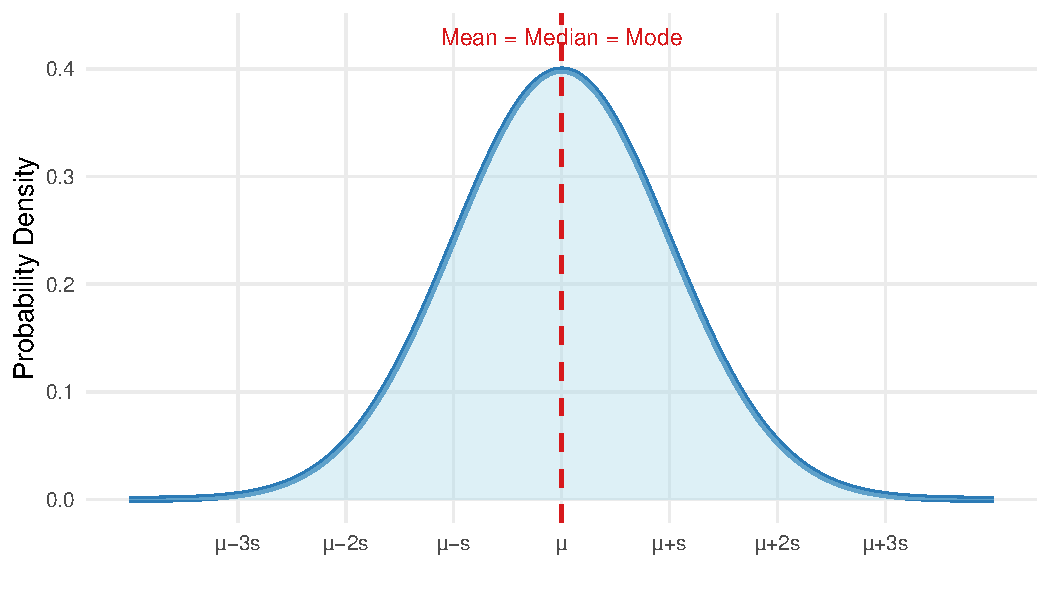
\includegraphics[keepaspectratio]{chapter03_probability_distribution_files/figure-pdf/fig-normal-intro-1.pdf}}

}

\caption{\label{fig-normal-intro}The Normal Distribution: a symmetric,
bell-shaped curve}

\end{figure}%

\begin{center}\rule{0.5\linewidth}{0.5pt}\end{center}

\section{Key Properties of the Normal
Distribution}\label{key-properties-of-the-normal-distribution}

A normal distribution is completely described by just \textbf{two
parameters}:

{\def\LTcaptype{none} % do not increment counter
\begin{longtable}[]{@{}
  >{\raggedright\arraybackslash}p{(\linewidth - 4\tabcolsep) * \real{0.2727}}
  >{\centering\arraybackslash}p{(\linewidth - 4\tabcolsep) * \real{0.4545}}
  >{\raggedright\arraybackslash}p{(\linewidth - 4\tabcolsep) * \real{0.2727}}@{}}
\toprule\noalign{}
\begin{minipage}[b]{\linewidth}\raggedright
Parameter
\end{minipage} & \begin{minipage}[b]{\linewidth}\centering
Symbol
\end{minipage} & \begin{minipage}[b]{\linewidth}\raggedright
Meaning
\end{minipage} \\
\midrule\noalign{}
\endhead
\bottomrule\noalign{}
\endlastfoot
Mean & \(\mu\) & Center of the distribution (peak of the bell) \\
Standard deviation & \(\sigma\) & Width of the bell --- larger σ =
wider, flatter curve \\
\end{longtable}
}

\textbf{Key properties:}

\begin{enumerate}
\def\labelenumi{\arabic{enumi}.}
\tightlist
\item
  \textbf{Symmetric} around the mean --- the left and right halves are
  mirror images
\item
  \textbf{Mean = Median = Mode} --- all three are equal and located at
  the center
\item
  The \textbf{total area} under the curve = 1 (representing 100\% of all
  probability)
\item
  The curve extends infinitely in both directions but never touches the
  x-axis
\end{enumerate}

\begin{center}\rule{0.5\linewidth}{0.5pt}\end{center}

\section{The 68--95--99.7 Rule (Empirical
Rule)}\label{the-689599.7-rule-empirical-rule}

One of the most useful facts about the normal distribution is how much
of the data falls within 1, 2, or 3 standard deviations of the mean.

\begin{Shaded}
\begin{Highlighting}[]
\NormalTok{x }\OtherTok{\textless{}{-}} \FunctionTok{seq}\NormalTok{(}\SpecialCharTok{{-}}\FloatTok{3.8}\NormalTok{, }\FloatTok{3.8}\NormalTok{, }\AttributeTok{length =} \DecValTok{1000}\NormalTok{)}
\NormalTok{y }\OtherTok{\textless{}{-}} \FunctionTok{dnorm}\NormalTok{(x)}
\NormalTok{df }\OtherTok{\textless{}{-}} \FunctionTok{data.frame}\NormalTok{(}\AttributeTok{x =}\NormalTok{ x, }\AttributeTok{y =}\NormalTok{ y)}

\FunctionTok{ggplot}\NormalTok{(df, }\FunctionTok{aes}\NormalTok{(x, y)) }\SpecialCharTok{+}
  \CommentTok{\# 3 SD shading}
  \FunctionTok{geom\_area}\NormalTok{(}\AttributeTok{data =} \FunctionTok{subset}\NormalTok{(df, x }\SpecialCharTok{\textgreater{}=} \SpecialCharTok{{-}}\DecValTok{3} \SpecialCharTok{\&}\NormalTok{ x }\SpecialCharTok{\textless{}=} \DecValTok{3}\NormalTok{),}
            \FunctionTok{aes}\NormalTok{(x, y), }\AttributeTok{fill =} \StringTok{"\#fdae61"}\NormalTok{, }\AttributeTok{alpha =} \FloatTok{0.5}\NormalTok{) }\SpecialCharTok{+}
  \CommentTok{\# 2 SD shading}
  \FunctionTok{geom\_area}\NormalTok{(}\AttributeTok{data =} \FunctionTok{subset}\NormalTok{(df, x }\SpecialCharTok{\textgreater{}=} \SpecialCharTok{{-}}\DecValTok{2} \SpecialCharTok{\&}\NormalTok{ x }\SpecialCharTok{\textless{}=} \DecValTok{2}\NormalTok{),}
            \FunctionTok{aes}\NormalTok{(x, y), }\AttributeTok{fill =} \StringTok{"\#abd9e9"}\NormalTok{, }\AttributeTok{alpha =} \FloatTok{0.6}\NormalTok{) }\SpecialCharTok{+}
  \CommentTok{\# 1 SD shading}
  \FunctionTok{geom\_area}\NormalTok{(}\AttributeTok{data =} \FunctionTok{subset}\NormalTok{(df, x }\SpecialCharTok{\textgreater{}=} \SpecialCharTok{{-}}\DecValTok{1} \SpecialCharTok{\&}\NormalTok{ x }\SpecialCharTok{\textless{}=} \DecValTok{1}\NormalTok{),}
            \FunctionTok{aes}\NormalTok{(x, y), }\AttributeTok{fill =} \StringTok{"\#2c7bb6"}\NormalTok{, }\AttributeTok{alpha =} \FloatTok{0.6}\NormalTok{) }\SpecialCharTok{+}
  \FunctionTok{geom\_line}\NormalTok{(}\AttributeTok{color =} \StringTok{"gray30"}\NormalTok{, }\AttributeTok{linewidth =} \FloatTok{1.2}\NormalTok{) }\SpecialCharTok{+}
  \CommentTok{\# Vertical lines}
  \FunctionTok{geom\_vline}\NormalTok{(}\AttributeTok{xintercept =} \FunctionTok{c}\NormalTok{(}\SpecialCharTok{{-}}\DecValTok{3}\NormalTok{,}\SpecialCharTok{{-}}\DecValTok{2}\NormalTok{,}\SpecialCharTok{{-}}\DecValTok{1}\NormalTok{,}\DecValTok{0}\NormalTok{,}\DecValTok{1}\NormalTok{,}\DecValTok{2}\NormalTok{,}\DecValTok{3}\NormalTok{),}
             \AttributeTok{linetype =} \StringTok{"dashed"}\NormalTok{, }\AttributeTok{color =} \StringTok{"gray50"}\NormalTok{, }\AttributeTok{linewidth =} \FloatTok{0.5}\NormalTok{) }\SpecialCharTok{+}
  \CommentTok{\# Percentage annotations}
  \FunctionTok{annotate}\NormalTok{(}\StringTok{"text"}\NormalTok{, }\AttributeTok{x =} \DecValTok{0}\NormalTok{, }\AttributeTok{y =} \FloatTok{0.20}\NormalTok{,}
           \AttributeTok{label =} \StringTok{"68\%"}\NormalTok{, }\AttributeTok{color =} \StringTok{"white"}\NormalTok{, }\AttributeTok{size =} \DecValTok{5}\NormalTok{, }\AttributeTok{fontface =} \StringTok{"bold"}\NormalTok{) }\SpecialCharTok{+}
  \FunctionTok{annotate}\NormalTok{(}\StringTok{"text"}\NormalTok{, }\AttributeTok{x =} \FloatTok{1.5}\NormalTok{, }\AttributeTok{y =} \FloatTok{0.07}\NormalTok{,}
           \AttributeTok{label =} \StringTok{"95\%"}\NormalTok{, }\AttributeTok{color =} \StringTok{"\#2c7bb6"}\NormalTok{, }\AttributeTok{size =} \FloatTok{4.5}\NormalTok{, }\AttributeTok{fontface =} \StringTok{"bold"}\NormalTok{) }\SpecialCharTok{+}
  \FunctionTok{annotate}\NormalTok{(}\StringTok{"text"}\NormalTok{, }\AttributeTok{x =} \FloatTok{2.5}\NormalTok{, }\AttributeTok{y =} \FloatTok{0.02}\NormalTok{,}
           \AttributeTok{label =} \StringTok{"99.7\%"}\NormalTok{, }\AttributeTok{color =} \StringTok{"\#d7191c"}\NormalTok{, }\AttributeTok{size =} \DecValTok{4}\NormalTok{, }\AttributeTok{fontface =} \StringTok{"bold"}\NormalTok{) }\SpecialCharTok{+}
  \FunctionTok{scale\_x\_continuous}\NormalTok{(}\AttributeTok{breaks =} \SpecialCharTok{{-}}\DecValTok{3}\SpecialCharTok{:}\DecValTok{3}\NormalTok{,}
                     \AttributeTok{labels =} \FunctionTok{c}\NormalTok{(}\StringTok{"μ−3σ"}\NormalTok{,}\StringTok{"μ−2σ"}\NormalTok{,}\StringTok{"μ−σ"}\NormalTok{,}\StringTok{"μ"}\NormalTok{,}\StringTok{"μ+σ"}\NormalTok{,}\StringTok{"μ+2σ"}\NormalTok{,}\StringTok{"μ+3σ"}\NormalTok{)) }\SpecialCharTok{+}
  \FunctionTok{labs}\NormalTok{(}\AttributeTok{x =} \StringTok{""}\NormalTok{, }\AttributeTok{y =} \StringTok{"Probability Density"}\NormalTok{,}
       \AttributeTok{caption =} \StringTok{"Blue = 68\% | Blue+Teal = 95\% | All shaded = 99.7\%"}\NormalTok{) }\SpecialCharTok{+}
  \FunctionTok{theme\_minimal}\NormalTok{(}\AttributeTok{base\_size =} \DecValTok{13}\NormalTok{) }\SpecialCharTok{+}
  \FunctionTok{theme}\NormalTok{(}\AttributeTok{panel.grid.minor =} \FunctionTok{element\_blank}\NormalTok{())}
\end{Highlighting}
\end{Shaded}

\begin{figure}[H]

\centering{

\pandocbounded{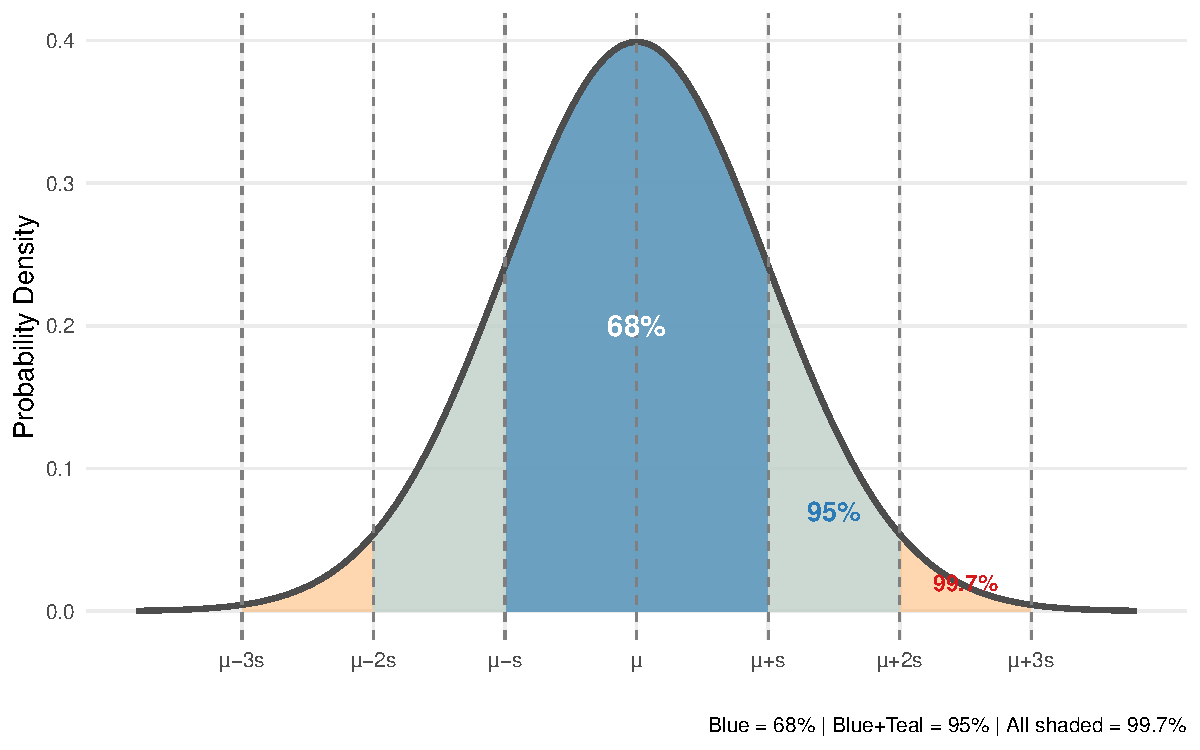
\includegraphics[keepaspectratio]{chapter03_probability_distribution_files/figure-pdf/fig-empirical-1.pdf}}

}

\caption{\label{fig-empirical}The 68--95--99.7 Rule for the Normal
Distribution}

\end{figure}%

\begin{tcolorbox}[enhanced jigsaw, arc=.35mm, bottomrule=.15mm, bottomtitle=1mm, breakable, colback=white, colbacktitle=quarto-callout-important-color!10!white, colframe=quarto-callout-important-color-frame, coltitle=black, left=2mm, leftrule=.75mm, opacityback=0, opacitybacktitle=0.6, rightrule=.15mm, title={📐 The Empirical Rule}, titlerule=0mm, toprule=.15mm, toptitle=1mm]

{\def\LTcaptype{none} % do not increment counter
\begin{longtable}[]{@{}lc@{}}
\toprule\noalign{}
Range & Proportion of data \\
\midrule\noalign{}
\endhead
\bottomrule\noalign{}
\endlastfoot
Within \textbf{1 SD} of the mean: \(\mu \pm \sigma\) & \textbf{≈
68\%} \\
Within \textbf{2 SD} of the mean: \(\mu \pm 2\sigma\) & \textbf{≈
95\%} \\
Within \textbf{3 SD} of the mean: \(\mu \pm 3\sigma\) & \textbf{≈
99.7\%} \\
\end{longtable}
}

This means only about \textbf{5\%} of values fall more than 2 SD from
the mean, and only \textbf{0.3\%} fall more than 3 SD away --- these are
considered unusual or extreme.

\end{tcolorbox}

\begin{center}\rule{0.5\linewidth}{0.5pt}\end{center}

\section{The Standard Normal Distribution and
Z-Score}\label{the-standard-normal-distribution-and-z-score}

\subsection{The Z-Score}\label{the-z-score}

Different normal distributions have different means and SDs. To compare
values across different distributions, we \textbf{standardize} them
using the \textbf{Z-score}:

\[z = \frac{x - \mu}{\sigma}\]

Where:

\begin{itemize}
\tightlist
\item
  \(x\) = the observed value
\item
  \(\mu\) = the population mean
\item
  \(\sigma\) = the population standard deviation
\item
  \(z\) = the number of standard deviations \(x\) is away from the mean
\end{itemize}

A \textbf{positive Z} means the value is above the mean; a
\textbf{negative Z} means it is below the mean.

\begin{center}\rule{0.5\linewidth}{0.5pt}\end{center}

\subsection{The Standard Normal
Distribution}\label{the-standard-normal-distribution}

When we convert all values to Z-scores, the resulting distribution is
called the \textbf{standard normal distribution}, with:

\[\mu = 0 \quad \text{and} \quad \sigma = 1\]

This is written as \(Z \sim N(0, 1)\).

\begin{Shaded}
\begin{Highlighting}[]
\NormalTok{x }\OtherTok{\textless{}{-}} \FunctionTok{seq}\NormalTok{(}\SpecialCharTok{{-}}\FloatTok{3.8}\NormalTok{, }\FloatTok{3.8}\NormalTok{, }\AttributeTok{length =} \DecValTok{500}\NormalTok{)}
\NormalTok{df }\OtherTok{\textless{}{-}} \FunctionTok{data.frame}\NormalTok{(}\AttributeTok{x =}\NormalTok{ x, }\AttributeTok{y =} \FunctionTok{dnorm}\NormalTok{(x))}

\FunctionTok{ggplot}\NormalTok{(df, }\FunctionTok{aes}\NormalTok{(x, y)) }\SpecialCharTok{+}
  \FunctionTok{geom\_area}\NormalTok{(}\AttributeTok{fill =} \StringTok{"\#abd9e9"}\NormalTok{, }\AttributeTok{alpha =} \FloatTok{0.5}\NormalTok{) }\SpecialCharTok{+}
  \FunctionTok{geom\_line}\NormalTok{(}\AttributeTok{color =} \StringTok{"\#2c7bb6"}\NormalTok{, }\AttributeTok{linewidth =} \FloatTok{1.3}\NormalTok{) }\SpecialCharTok{+}
  \FunctionTok{geom\_vline}\NormalTok{(}\AttributeTok{xintercept =} \DecValTok{0}\NormalTok{, }\AttributeTok{linetype =} \StringTok{"dashed"}\NormalTok{,}
             \AttributeTok{color =} \StringTok{"\#d7191c"}\NormalTok{, }\AttributeTok{linewidth =} \DecValTok{1}\NormalTok{) }\SpecialCharTok{+}
  \FunctionTok{scale\_x\_continuous}\NormalTok{(}\AttributeTok{breaks =} \SpecialCharTok{{-}}\DecValTok{3}\SpecialCharTok{:}\DecValTok{3}\NormalTok{) }\SpecialCharTok{+}
  \FunctionTok{labs}\NormalTok{(}\AttributeTok{x =} \StringTok{"Z"}\NormalTok{, }\AttributeTok{y =} \StringTok{"Probability Density"}\NormalTok{,}
       \AttributeTok{title =} \StringTok{"Standard Normal Distribution: N(0, 1)"}\NormalTok{) }\SpecialCharTok{+}
  \FunctionTok{theme\_minimal}\NormalTok{(}\AttributeTok{base\_size =} \DecValTok{13}\NormalTok{) }\SpecialCharTok{+}
  \FunctionTok{theme}\NormalTok{(}\AttributeTok{panel.grid.minor =} \FunctionTok{element\_blank}\NormalTok{(),}
        \AttributeTok{plot.title =} \FunctionTok{element\_text}\NormalTok{(}\AttributeTok{hjust =} \FloatTok{0.5}\NormalTok{, }\AttributeTok{face =} \StringTok{"bold"}\NormalTok{))}
\end{Highlighting}
\end{Shaded}

\begin{figure}[H]

\centering{

\pandocbounded{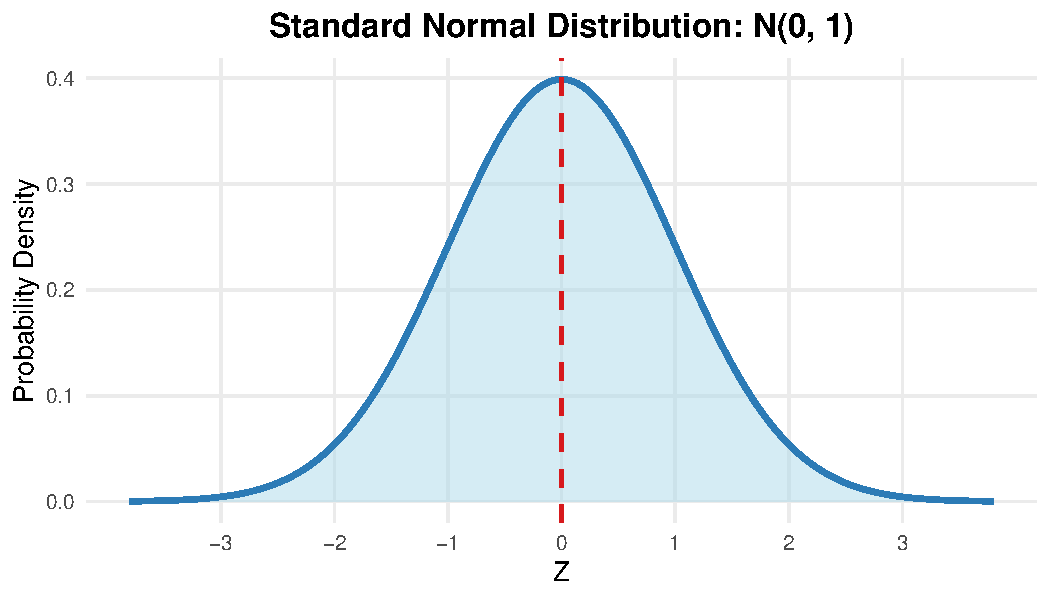
\includegraphics[keepaspectratio]{chapter03_probability_distribution_files/figure-pdf/fig-znorm-1.pdf}}

}

\caption{\label{fig-znorm}Standard Normal Distribution N(0,1)}

\end{figure}%

\begin{center}\rule{0.5\linewidth}{0.5pt}\end{center}

\subsection{Finding Probabilities Using the
Z-Table}\label{finding-probabilities-using-the-z-table}

The \textbf{Z-table} (also called the standard normal table) gives us
the \textbf{area to the left} of any Z-score --- which equals the
\textbf{probability} that a randomly selected observation falls below
that value.

\begin{Shaded}
\begin{Highlighting}[]
\NormalTok{z\_vals }\OtherTok{\textless{}{-}} \FunctionTok{seq}\NormalTok{(}\FloatTok{0.0}\NormalTok{, }\FloatTok{2.0}\NormalTok{, }\AttributeTok{by =} \FloatTok{0.1}\NormalTok{)}
\NormalTok{decimals }\OtherTok{\textless{}{-}} \FunctionTok{seq}\NormalTok{(}\FloatTok{0.00}\NormalTok{, }\FloatTok{0.09}\NormalTok{, }\AttributeTok{by =} \FloatTok{0.01}\NormalTok{)}

\NormalTok{z\_matrix }\OtherTok{\textless{}{-}} \FunctionTok{outer}\NormalTok{(z\_vals, decimals, }\ControlFlowTok{function}\NormalTok{(z, d) \{}
  \FunctionTok{round}\NormalTok{(}\FunctionTok{pnorm}\NormalTok{(z }\SpecialCharTok{+}\NormalTok{ d), }\DecValTok{4}\NormalTok{)}
\NormalTok{\})}

\FunctionTok{rownames}\NormalTok{(z\_matrix) }\OtherTok{\textless{}{-}} \FunctionTok{formatC}\NormalTok{(z\_vals, }\AttributeTok{format =} \StringTok{"f"}\NormalTok{, }\AttributeTok{digits =} \DecValTok{1}\NormalTok{)}
\FunctionTok{colnames}\NormalTok{(z\_matrix) }\OtherTok{\textless{}{-}} \FunctionTok{formatC}\NormalTok{(decimals, }\AttributeTok{format =} \StringTok{"f"}\NormalTok{, }\AttributeTok{digits =} \DecValTok{2}\NormalTok{)}

\FunctionTok{kable}\NormalTok{(z\_matrix, }\AttributeTok{caption =} \StringTok{"Area to the left of Z (rows = Z integer + 1st decimal, columns = 2nd decimal)"}\NormalTok{) }\SpecialCharTok{|\textgreater{}}
  \FunctionTok{kable\_styling}\NormalTok{(}\AttributeTok{bootstrap\_options =} \FunctionTok{c}\NormalTok{(}\StringTok{"striped"}\NormalTok{,}\StringTok{"hover"}\NormalTok{,}\StringTok{"condensed"}\NormalTok{),}
                \AttributeTok{full\_width =} \ConstantTok{TRUE}\NormalTok{, }\AttributeTok{font\_size =} \DecValTok{11}\NormalTok{) }\SpecialCharTok{|\textgreater{}}
  \FunctionTok{column\_spec}\NormalTok{(}\DecValTok{1}\NormalTok{, }\AttributeTok{bold =} \ConstantTok{TRUE}\NormalTok{, }\AttributeTok{color =} \StringTok{"\#2c7bb6"}\NormalTok{)}
\end{Highlighting}
\end{Shaded}

\begin{table}

\caption{\label{tbl-ztable}Standard Normal Table (area to the LEFT of
Z)}

\centering{

\begingroup\fontsize{11}{13}\selectfont

\begin{longtabu} to \linewidth {>{}l>{\raggedleft}X>{\raggedleft}X>{\raggedleft}X>{\raggedleft}X>{\raggedleft}X>{\raggedleft}X>{\raggedleft}X>{\raggedleft}X>{\raggedleft}X>{\raggedleft}X}
\caption{\label{tab:tbl-ztable}Area to the left of Z (rows = Z integer + 1st decimal, columns = 2nd decimal)}\\
\toprule
 & 0.00 & 0.01 & 0.02 & 0.03 & 0.04 & 0.05 & 0.06 & 0.07 & 0.08 & 0.09\\
\midrule
\textcolor[HTML]{2c7bb6}{\textbf{0.0}} & 0.5000 & 0.5040 & 0.5080 & 0.5120 & 0.5160 & 0.5199 & 0.5239 & 0.5279 & 0.5319 & 0.5359\\
\textcolor[HTML]{2c7bb6}{\textbf{0.1}} & 0.5398 & 0.5438 & 0.5478 & 0.5517 & 0.5557 & 0.5596 & 0.5636 & 0.5675 & 0.5714 & 0.5753\\
\textcolor[HTML]{2c7bb6}{\textbf{0.2}} & 0.5793 & 0.5832 & 0.5871 & 0.5910 & 0.5948 & 0.5987 & 0.6026 & 0.6064 & 0.6103 & 0.6141\\
\textcolor[HTML]{2c7bb6}{\textbf{0.3}} & 0.6179 & 0.6217 & 0.6255 & 0.6293 & 0.6331 & 0.6368 & 0.6406 & 0.6443 & 0.6480 & 0.6517\\
\textcolor[HTML]{2c7bb6}{\textbf{0.4}} & 0.6554 & 0.6591 & 0.6628 & 0.6664 & 0.6700 & 0.6736 & 0.6772 & 0.6808 & 0.6844 & 0.6879\\
\addlinespace
\textcolor[HTML]{2c7bb6}{\textbf{0.5}} & 0.6915 & 0.6950 & 0.6985 & 0.7019 & 0.7054 & 0.7088 & 0.7123 & 0.7157 & 0.7190 & 0.7224\\
\textcolor[HTML]{2c7bb6}{\textbf{0.6}} & 0.7257 & 0.7291 & 0.7324 & 0.7357 & 0.7389 & 0.7422 & 0.7454 & 0.7486 & 0.7517 & 0.7549\\
\textcolor[HTML]{2c7bb6}{\textbf{0.7}} & 0.7580 & 0.7611 & 0.7642 & 0.7673 & 0.7704 & 0.7734 & 0.7764 & 0.7794 & 0.7823 & 0.7852\\
\textcolor[HTML]{2c7bb6}{\textbf{0.8}} & 0.7881 & 0.7910 & 0.7939 & 0.7967 & 0.7995 & 0.8023 & 0.8051 & 0.8078 & 0.8106 & 0.8133\\
\textcolor[HTML]{2c7bb6}{\textbf{0.9}} & 0.8159 & 0.8186 & 0.8212 & 0.8238 & 0.8264 & 0.8289 & 0.8315 & 0.8340 & 0.8365 & 0.8389\\
\addlinespace
\textcolor[HTML]{2c7bb6}{\textbf{1.0}} & 0.8413 & 0.8438 & 0.8461 & 0.8485 & 0.8508 & 0.8531 & 0.8554 & 0.8577 & 0.8599 & 0.8621\\
\textcolor[HTML]{2c7bb6}{\textbf{1.1}} & 0.8643 & 0.8665 & 0.8686 & 0.8708 & 0.8729 & 0.8749 & 0.8770 & 0.8790 & 0.8810 & 0.8830\\
\textcolor[HTML]{2c7bb6}{\textbf{1.2}} & 0.8849 & 0.8869 & 0.8888 & 0.8907 & 0.8925 & 0.8944 & 0.8962 & 0.8980 & 0.8997 & 0.9015\\
\textcolor[HTML]{2c7bb6}{\textbf{1.3}} & 0.9032 & 0.9049 & 0.9066 & 0.9082 & 0.9099 & 0.9115 & 0.9131 & 0.9147 & 0.9162 & 0.9177\\
\textcolor[HTML]{2c7bb6}{\textbf{1.4}} & 0.9192 & 0.9207 & 0.9222 & 0.9236 & 0.9251 & 0.9265 & 0.9279 & 0.9292 & 0.9306 & 0.9319\\
\addlinespace
\textcolor[HTML]{2c7bb6}{\textbf{1.5}} & 0.9332 & 0.9345 & 0.9357 & 0.9370 & 0.9382 & 0.9394 & 0.9406 & 0.9418 & 0.9429 & 0.9441\\
\textcolor[HTML]{2c7bb6}{\textbf{1.6}} & 0.9452 & 0.9463 & 0.9474 & 0.9484 & 0.9495 & 0.9505 & 0.9515 & 0.9525 & 0.9535 & 0.9545\\
\textcolor[HTML]{2c7bb6}{\textbf{1.7}} & 0.9554 & 0.9564 & 0.9573 & 0.9582 & 0.9591 & 0.9599 & 0.9608 & 0.9616 & 0.9625 & 0.9633\\
\textcolor[HTML]{2c7bb6}{\textbf{1.8}} & 0.9641 & 0.9649 & 0.9656 & 0.9664 & 0.9671 & 0.9678 & 0.9686 & 0.9693 & 0.9699 & 0.9706\\
\textcolor[HTML]{2c7bb6}{\textbf{1.9}} & 0.9713 & 0.9719 & 0.9726 & 0.9732 & 0.9738 & 0.9744 & 0.9750 & 0.9756 & 0.9761 & 0.9767\\
\addlinespace
\textcolor[HTML]{2c7bb6}{\textbf{2.0}} & 0.9772 & 0.9778 & 0.9783 & 0.9788 & 0.9793 & 0.9798 & 0.9803 & 0.9808 & 0.9812 & 0.9817\\
\bottomrule
\end{longtabu}
\endgroup{}

}

\end{table}%

\textbf{How to use the table:} To find \(P(Z < 1.23)\), look at row
\textbf{1.2} and column \textbf{0.03} → read off the value.

\begin{center}\rule{0.5\linewidth}{0.5pt}\end{center}

\subsection{Common Z-Table Probability
Rules}\label{common-z-table-probability-rules}

\begin{Shaded}
\begin{Highlighting}[]
\NormalTok{x }\OtherTok{\textless{}{-}} \FunctionTok{seq}\NormalTok{(}\SpecialCharTok{{-}}\FloatTok{3.5}\NormalTok{, }\FloatTok{3.5}\NormalTok{, }\AttributeTok{length =} \DecValTok{500}\NormalTok{)}
\NormalTok{y }\OtherTok{\textless{}{-}} \FunctionTok{dnorm}\NormalTok{(x)}
\NormalTok{df }\OtherTok{\textless{}{-}} \FunctionTok{data.frame}\NormalTok{(}\AttributeTok{x =}\NormalTok{ x, }\AttributeTok{y =}\NormalTok{ y)}
\NormalTok{z\_val }\OtherTok{\textless{}{-}} \FloatTok{1.5}

\NormalTok{p1 }\OtherTok{\textless{}{-}} \FunctionTok{ggplot}\NormalTok{(df, }\FunctionTok{aes}\NormalTok{(x, y)) }\SpecialCharTok{+}
  \FunctionTok{geom\_area}\NormalTok{(}\AttributeTok{data =} \FunctionTok{subset}\NormalTok{(df, x }\SpecialCharTok{\textless{}=}\NormalTok{ z\_val), }\AttributeTok{fill =} \StringTok{"\#2c7bb6"}\NormalTok{, }\AttributeTok{alpha =} \FloatTok{0.6}\NormalTok{) }\SpecialCharTok{+}
  \FunctionTok{geom\_line}\NormalTok{(}\AttributeTok{linewidth =} \DecValTok{1}\NormalTok{) }\SpecialCharTok{+}
  \FunctionTok{geom\_vline}\NormalTok{(}\AttributeTok{xintercept =}\NormalTok{ z\_val, }\AttributeTok{linetype =} \StringTok{"dashed"}\NormalTok{, }\AttributeTok{color =} \StringTok{"\#d7191c"}\NormalTok{) }\SpecialCharTok{+}
  \FunctionTok{annotate}\NormalTok{(}\StringTok{"text"}\NormalTok{, }\AttributeTok{x =} \SpecialCharTok{{-}}\DecValTok{1}\NormalTok{, }\AttributeTok{y =} \FloatTok{0.15}\NormalTok{,}
           \AttributeTok{label =} \FunctionTok{paste0}\NormalTok{(}\StringTok{"P(Z \textless{} "}\NormalTok{, z\_val, }\StringTok{")"}\NormalTok{), }\AttributeTok{size =} \FloatTok{3.5}\NormalTok{, }\AttributeTok{color =} \StringTok{"white"}\NormalTok{) }\SpecialCharTok{+}
  \FunctionTok{labs}\NormalTok{(}\AttributeTok{title =} \StringTok{"P(Z \textless{} z)"}\NormalTok{, }\AttributeTok{x =} \StringTok{"Z"}\NormalTok{, }\AttributeTok{y =} \StringTok{""}\NormalTok{) }\SpecialCharTok{+}
  \FunctionTok{scale\_x\_continuous}\NormalTok{(}\AttributeTok{breaks =} \FunctionTok{c}\NormalTok{(}\DecValTok{0}\NormalTok{, z\_val),}
                     \AttributeTok{labels =} \FunctionTok{c}\NormalTok{(}\StringTok{"0"}\NormalTok{, }\FunctionTok{paste0}\NormalTok{(}\StringTok{"z="}\NormalTok{,z\_val))) }\SpecialCharTok{+}
  \FunctionTok{theme\_minimal}\NormalTok{(}\AttributeTok{base\_size =} \DecValTok{11}\NormalTok{) }\SpecialCharTok{+}
  \FunctionTok{theme}\NormalTok{(}\AttributeTok{panel.grid =} \FunctionTok{element\_blank}\NormalTok{())}

\NormalTok{p2 }\OtherTok{\textless{}{-}} \FunctionTok{ggplot}\NormalTok{(df, }\FunctionTok{aes}\NormalTok{(x, y)) }\SpecialCharTok{+}
  \FunctionTok{geom\_area}\NormalTok{(}\AttributeTok{data =} \FunctionTok{subset}\NormalTok{(df, x }\SpecialCharTok{\textgreater{}=}\NormalTok{ z\_val), }\AttributeTok{fill =} \StringTok{"\#d7191c"}\NormalTok{, }\AttributeTok{alpha =} \FloatTok{0.6}\NormalTok{) }\SpecialCharTok{+}
  \FunctionTok{geom\_line}\NormalTok{(}\AttributeTok{linewidth =} \DecValTok{1}\NormalTok{) }\SpecialCharTok{+}
  \FunctionTok{geom\_vline}\NormalTok{(}\AttributeTok{xintercept =}\NormalTok{ z\_val, }\AttributeTok{linetype =} \StringTok{"dashed"}\NormalTok{, }\AttributeTok{color =} \StringTok{"\#d7191c"}\NormalTok{) }\SpecialCharTok{+}
  \FunctionTok{annotate}\NormalTok{(}\StringTok{"text"}\NormalTok{, }\AttributeTok{x =} \FloatTok{2.5}\NormalTok{, }\AttributeTok{y =} \FloatTok{0.15}\NormalTok{,}
           \AttributeTok{label =} \FunctionTok{paste0}\NormalTok{(}\StringTok{"P(Z \textgreater{} "}\NormalTok{, z\_val, }\StringTok{")"}\NormalTok{), }\AttributeTok{size =} \FloatTok{3.5}\NormalTok{, }\AttributeTok{color =} \StringTok{"white"}\NormalTok{) }\SpecialCharTok{+}
  \FunctionTok{labs}\NormalTok{(}\AttributeTok{title =} \StringTok{"P(Z \textgreater{} z) = 1 − P(Z \textless{} z)"}\NormalTok{, }\AttributeTok{x =} \StringTok{"Z"}\NormalTok{, }\AttributeTok{y =} \StringTok{""}\NormalTok{) }\SpecialCharTok{+}
  \FunctionTok{scale\_x\_continuous}\NormalTok{(}\AttributeTok{breaks =} \FunctionTok{c}\NormalTok{(}\DecValTok{0}\NormalTok{, z\_val),}
                     \AttributeTok{labels =} \FunctionTok{c}\NormalTok{(}\StringTok{"0"}\NormalTok{, }\FunctionTok{paste0}\NormalTok{(}\StringTok{"z="}\NormalTok{,z\_val))) }\SpecialCharTok{+}
  \FunctionTok{theme\_minimal}\NormalTok{(}\AttributeTok{base\_size =} \DecValTok{11}\NormalTok{) }\SpecialCharTok{+}
  \FunctionTok{theme}\NormalTok{(}\AttributeTok{panel.grid =} \FunctionTok{element\_blank}\NormalTok{())}

\NormalTok{p3 }\OtherTok{\textless{}{-}} \FunctionTok{ggplot}\NormalTok{(df, }\FunctionTok{aes}\NormalTok{(x, y)) }\SpecialCharTok{+}
  \FunctionTok{geom\_area}\NormalTok{(}\AttributeTok{data =} \FunctionTok{subset}\NormalTok{(df, x }\SpecialCharTok{\textgreater{}=} \SpecialCharTok{{-}}\NormalTok{z\_val }\SpecialCharTok{\&}\NormalTok{ x }\SpecialCharTok{\textless{}=}\NormalTok{ z\_val),}
            \AttributeTok{fill =} \StringTok{"\#1a9641"}\NormalTok{, }\AttributeTok{alpha =} \FloatTok{0.6}\NormalTok{) }\SpecialCharTok{+}
  \FunctionTok{geom\_line}\NormalTok{(}\AttributeTok{linewidth =} \DecValTok{1}\NormalTok{) }\SpecialCharTok{+}
  \FunctionTok{geom\_vline}\NormalTok{(}\AttributeTok{xintercept =} \FunctionTok{c}\NormalTok{(}\SpecialCharTok{{-}}\NormalTok{z\_val, z\_val),}
             \AttributeTok{linetype =} \StringTok{"dashed"}\NormalTok{, }\AttributeTok{color =} \StringTok{"\#d7191c"}\NormalTok{) }\SpecialCharTok{+}
  \FunctionTok{annotate}\NormalTok{(}\StringTok{"text"}\NormalTok{, }\AttributeTok{x =} \DecValTok{0}\NormalTok{, }\AttributeTok{y =} \FloatTok{0.15}\NormalTok{,}
           \AttributeTok{label =} \StringTok{"P(−z \textless{} Z \textless{} z)"}\NormalTok{, }\AttributeTok{size =} \FloatTok{3.5}\NormalTok{, }\AttributeTok{color =} \StringTok{"white"}\NormalTok{) }\SpecialCharTok{+}
  \FunctionTok{labs}\NormalTok{(}\AttributeTok{title =} \StringTok{"P(z₁ \textless{} Z \textless{} z₂)"}\NormalTok{, }\AttributeTok{x =} \StringTok{"Z"}\NormalTok{, }\AttributeTok{y =} \StringTok{""}\NormalTok{) }\SpecialCharTok{+}
  \FunctionTok{scale\_x\_continuous}\NormalTok{(}\AttributeTok{breaks =} \FunctionTok{c}\NormalTok{(}\SpecialCharTok{{-}}\NormalTok{z\_val, }\DecValTok{0}\NormalTok{, z\_val),}
                     \AttributeTok{labels =} \FunctionTok{c}\NormalTok{(}\FunctionTok{paste0}\NormalTok{(}\StringTok{"{-}"}\NormalTok{,z\_val), }\StringTok{"0"}\NormalTok{, z\_val)) }\SpecialCharTok{+}
  \FunctionTok{theme\_minimal}\NormalTok{(}\AttributeTok{base\_size =} \DecValTok{11}\NormalTok{) }\SpecialCharTok{+}
  \FunctionTok{theme}\NormalTok{(}\AttributeTok{panel.grid =} \FunctionTok{element\_blank}\NormalTok{())}

\FunctionTok{library}\NormalTok{(patchwork)}
\NormalTok{p1 }\SpecialCharTok{+}\NormalTok{ p2 }\SpecialCharTok{+}\NormalTok{ p3}
\end{Highlighting}
\end{Shaded}

\begin{figure}[H]

\centering{

\pandocbounded{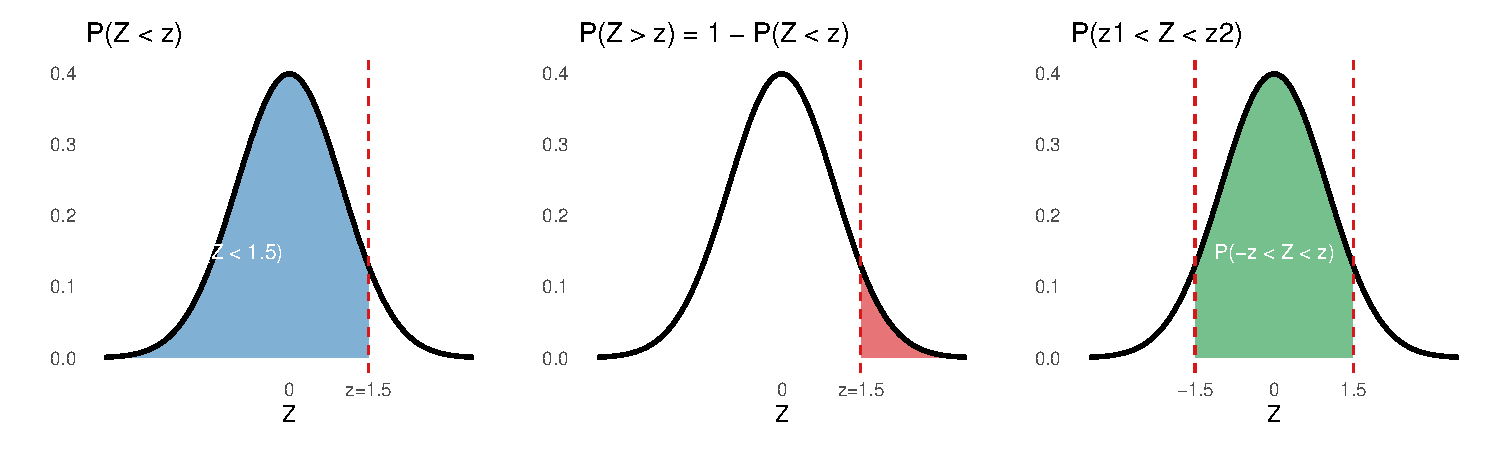
\includegraphics[keepaspectratio]{chapter03_probability_distribution_files/figure-pdf/fig-z-rules-1.pdf}}

}

\caption{\label{fig-z-rules}Three useful probability rules for the
normal distribution}

\end{figure}%

\begin{tcolorbox}[enhanced jigsaw, arc=.35mm, bottomrule=.15mm, bottomtitle=1mm, breakable, colback=white, colbacktitle=quarto-callout-important-color!10!white, colframe=quarto-callout-important-color-frame, coltitle=black, left=2mm, leftrule=.75mm, opacityback=0, opacitybacktitle=0.6, rightrule=.15mm, title={📐 Key Probability Rules}, titlerule=0mm, toprule=.15mm, toptitle=1mm]

{\def\LTcaptype{none} % do not increment counter
\begin{longtable}[]{@{}
  >{\raggedright\arraybackslash}p{(\linewidth - 2\tabcolsep) * \real{0.5000}}
  >{\raggedright\arraybackslash}p{(\linewidth - 2\tabcolsep) * \real{0.5000}}@{}}
\toprule\noalign{}
\begin{minipage}[b]{\linewidth}\raggedright
Situation
\end{minipage} & \begin{minipage}[b]{\linewidth}\raggedright
Formula
\end{minipage} \\
\midrule\noalign{}
\endhead
\bottomrule\noalign{}
\endlastfoot
Probability \textbf{below} z & \(P(Z < z)\) --- read directly from
Z-table \\
Probability \textbf{above} z & \(P(Z > z) = 1 - P(Z < z)\) \\
Probability \textbf{between} two values &
\(P(z_1 < Z < z_2) = P(Z < z_2) - P(Z < z_1)\) \\
\end{longtable}
}

\end{tcolorbox}

\begin{center}\rule{0.5\linewidth}{0.5pt}\end{center}

\bookmarksetup{startatroot}

\chapter{Key Takeaways}\label{key-takeaways-2}

\begin{tcolorbox}[enhanced jigsaw, arc=.35mm, bottomrule=.15mm, bottomtitle=1mm, breakable, colback=white, colbacktitle=quarto-callout-note-color!10!white, colframe=quarto-callout-note-color-frame, coltitle=black, left=2mm, leftrule=.75mm, opacityback=0, opacitybacktitle=0.6, rightrule=.15mm, title={📝 Chapter 3 Summary}, titlerule=0mm, toprule=.15mm, toptitle=1mm]

\begin{enumerate}
\def\labelenumi{\arabic{enumi}.}
\item
  A \textbf{frequency distribution} organizes data into a table showing
  how often each value or range of values occurs. It can show absolute
  frequency, relative frequency, or cumulative frequency.
\item
  The \textbf{normal distribution} is a symmetric, bell-shaped
  distribution described by its mean (\(\mu\)) and standard deviation
  (\(\sigma\)).
\item
  The \textbf{68--95--99.7 rule}: approximately 68\%, 95\%, and 99.7\%
  of values fall within 1, 2, and 3 standard deviations of the mean,
  respectively.
\item
  A \textbf{Z-score} measures how many standard deviations a value is
  from the mean: \(z = \dfrac{x - \mu}{\sigma}\)
\item
  The \textbf{Z-table} gives the probability (area) to the left of any
  Z-score, allowing us to find the probability that a measurement falls
  in any range.
\end{enumerate}

\end{tcolorbox}

\begin{center}\rule{0.5\linewidth}{0.5pt}\end{center}

\bookmarksetup{startatroot}

\chapter{Examples}\label{examples-2}

\section{Example 1: Constructing a Frequency Distribution
Table}\label{example-1-constructing-a-frequency-distribution-table}

The following are the ages (in years) of 20 patients:

\[45, 62, 38, 55, 71, 48, 60, 33, 52, 67,\]
\[41, 58, 74, 50, 65, 44, 57, 69, 36, 53\]

Construct a frequency distribution table using \textbf{5 class
intervals}.

\begin{tcolorbox}[enhanced jigsaw, arc=.35mm, bottomrule=.15mm, bottomtitle=1mm, breakable, colback=white, colbacktitle=quarto-callout-tip-color!10!white, colframe=quarto-callout-tip-color-frame, coltitle=black, left=2mm, leftrule=.75mm, opacityback=0, opacitybacktitle=0.6, rightrule=.15mm, title={✅ Solution}, titlerule=0mm, toprule=.15mm, toptitle=1mm]

\textbf{Step 1 --- Find the range:} \[\text{Range} = 74 - 33 = 41\]

\textbf{Step 2 --- Calculate class width:}
\[\text{Class width} = \frac{41}{5} = 8.2 \rightarrow \text{round up to } 9\]

\textbf{Step 3 --- Construct the table} (starting from 33):

\begin{Shaded}
\begin{Highlighting}[]
\NormalTok{ages }\OtherTok{\textless{}{-}} \FunctionTok{c}\NormalTok{(}\DecValTok{45}\NormalTok{,}\DecValTok{62}\NormalTok{,}\DecValTok{38}\NormalTok{,}\DecValTok{55}\NormalTok{,}\DecValTok{71}\NormalTok{,}\DecValTok{48}\NormalTok{,}\DecValTok{60}\NormalTok{,}\DecValTok{33}\NormalTok{,}\DecValTok{52}\NormalTok{,}\DecValTok{67}\NormalTok{,}\DecValTok{41}\NormalTok{,}\DecValTok{58}\NormalTok{,}\DecValTok{74}\NormalTok{,}\DecValTok{50}\NormalTok{,}\DecValTok{65}\NormalTok{,}\DecValTok{44}\NormalTok{,}\DecValTok{57}\NormalTok{,}\DecValTok{69}\NormalTok{,}\DecValTok{36}\NormalTok{,}\DecValTok{53}\NormalTok{)}
\NormalTok{breaks2 }\OtherTok{\textless{}{-}} \FunctionTok{c}\NormalTok{(}\DecValTok{33}\NormalTok{, }\DecValTok{42}\NormalTok{, }\DecValTok{51}\NormalTok{, }\DecValTok{60}\NormalTok{, }\DecValTok{69}\NormalTok{, }\DecValTok{78}\NormalTok{)}
\NormalTok{labels2 }\OtherTok{\textless{}{-}} \FunctionTok{c}\NormalTok{(}\StringTok{"33–41"}\NormalTok{,}\StringTok{"42–50"}\NormalTok{,}\StringTok{"51–59"}\NormalTok{,}\StringTok{"60–68"}\NormalTok{,}\StringTok{"69–77"}\NormalTok{)}
\NormalTok{age\_cut }\OtherTok{\textless{}{-}} \FunctionTok{cut}\NormalTok{(ages, }\AttributeTok{breaks =}\NormalTok{ breaks2, }\AttributeTok{right =} \ConstantTok{TRUE}\NormalTok{, }\AttributeTok{labels =}\NormalTok{ labels2,}
               \AttributeTok{include.lowest =} \ConstantTok{TRUE}\NormalTok{)}
\NormalTok{ft }\OtherTok{\textless{}{-}} \FunctionTok{as.data.frame}\NormalTok{(}\FunctionTok{table}\NormalTok{(age\_cut))}
\FunctionTok{colnames}\NormalTok{(ft) }\OtherTok{\textless{}{-}} \FunctionTok{c}\NormalTok{(}\StringTok{"Age Group (years)"}\NormalTok{, }\StringTok{"Frequency (f)"}\NormalTok{)}
\NormalTok{ft}\SpecialCharTok{$}\StringTok{\textasciigrave{}}\AttributeTok{Relative Frequency}\StringTok{\textasciigrave{}} \OtherTok{\textless{}{-}} \FunctionTok{round}\NormalTok{(ft}\SpecialCharTok{$}\StringTok{\textasciigrave{}}\AttributeTok{Frequency (f)}\StringTok{\textasciigrave{}} \SpecialCharTok{/} \DecValTok{20}\NormalTok{, }\DecValTok{2}\NormalTok{)}
\NormalTok{ft}\SpecialCharTok{$}\NormalTok{Percentage }\OtherTok{\textless{}{-}} \FunctionTok{paste0}\NormalTok{(ft}\SpecialCharTok{$}\StringTok{\textasciigrave{}}\AttributeTok{Relative Frequency}\StringTok{\textasciigrave{}} \SpecialCharTok{*} \DecValTok{100}\NormalTok{, }\StringTok{"\%"}\NormalTok{)}
\NormalTok{ft}\SpecialCharTok{$}\StringTok{\textasciigrave{}}\AttributeTok{Cumulative Frequency}\StringTok{\textasciigrave{}} \OtherTok{\textless{}{-}} \FunctionTok{cumsum}\NormalTok{(ft}\SpecialCharTok{$}\StringTok{\textasciigrave{}}\AttributeTok{Frequency (f)}\StringTok{\textasciigrave{}}\NormalTok{)}

\FunctionTok{kable}\NormalTok{(ft, }\AttributeTok{align =} \FunctionTok{c}\NormalTok{(}\StringTok{"c"}\NormalTok{,}\StringTok{"c"}\NormalTok{,}\StringTok{"c"}\NormalTok{,}\StringTok{"c"}\NormalTok{,}\StringTok{"c"}\NormalTok{)) }\SpecialCharTok{|\textgreater{}}
  \FunctionTok{kable\_styling}\NormalTok{(}\AttributeTok{bootstrap\_options =} \FunctionTok{c}\NormalTok{(}\StringTok{"striped"}\NormalTok{,}\StringTok{"hover"}\NormalTok{,}\StringTok{"bordered"}\NormalTok{),}
                \AttributeTok{full\_width =} \ConstantTok{FALSE}\NormalTok{, }\AttributeTok{font\_size =} \DecValTok{13}\NormalTok{) }\SpecialCharTok{|\textgreater{}}
  \FunctionTok{column\_spec}\NormalTok{(}\DecValTok{1}\NormalTok{, }\AttributeTok{bold =} \ConstantTok{TRUE}\NormalTok{)}
\end{Highlighting}
\end{Shaded}

\begingroup\fontsize{13}{15}\selectfont

\begin{longtable}[t]{>{}ccccc}

\caption{\label{tbl-ex1}Frequency Distribution of Patient Ages (n = 20)}

\tabularnewline

\toprule
Age Group (years) & Frequency (f) & Relative Frequency & Percentage & Cumulative Frequency\\
\midrule
\textbf{33–41} & 4 & 0.2 & 20\% & 4\\
\textbf{42–50} & 4 & 0.2 & 20\% & 8\\
\textbf{51–59} & 6 & 0.3 & 30\% & 14\\
\textbf{60–68} & 4 & 0.2 & 20\% & 18\\
\textbf{69–77} & 2 & 0.1 & 10\% & 20\\
\bottomrule

\end{longtable}

\endgroup{}

\textbf{Interpretation:} The largest group of patients is aged
\textbf{51--59 years} (6 patients, 30\%). Half of all patients
(cumulative frequency = 10) are aged 50 years or younger.

\end{tcolorbox}

\begin{center}\rule{0.5\linewidth}{0.5pt}\end{center}

\section{Example 2: Applying the Empirical
Rule}\label{example-2-applying-the-empirical-rule}

The systolic blood pressure (SBP) of adults in a community follows a
normal distribution with \textbf{mean = 125 mmHg} and \textbf{SD = 14
mmHg}.

\textbf{(a)} Between what two values does the SBP of the \textbf{middle
95\%} of adults fall?

\textbf{(b)} What percentage of adults have SBP \textbf{above 153 mmHg}?

\begin{tcolorbox}[enhanced jigsaw, arc=.35mm, bottomrule=.15mm, bottomtitle=1mm, breakable, colback=white, colbacktitle=quarto-callout-tip-color!10!white, colframe=quarto-callout-tip-color-frame, coltitle=black, left=2mm, leftrule=.75mm, opacityback=0, opacitybacktitle=0.6, rightrule=.15mm, title={✅ Solution}, titlerule=0mm, toprule=.15mm, toptitle=1mm]

\textbf{(a)} The middle 95\% falls within \(\mu \pm 2\sigma\):

\[125 - 2(14) = 97 \text{ mmHg} \quad \text{to} \quad 125 + 2(14) = 153 \text{ mmHg}\]

So \textbf{95\% of adults} have SBP between \textbf{97 and 153 mmHg}.

\textbf{(b)} SBP = 153 mmHg is exactly \(\mu + 2\sigma\). Since 95\% of
values fall \emph{within} 2 SD, the remaining 5\% fall \emph{outside}.
By symmetry, \textbf{2.5\%} fall above 153 mmHg and 2.5\% fall below 97
mmHg.

\textbf{Answer:} Approximately \textbf{2.5\%} of adults have SBP above
153 mmHg.

\end{tcolorbox}

\begin{center}\rule{0.5\linewidth}{0.5pt}\end{center}

\section{Example 3: Using Z-Scores and the
Z-Table}\label{example-3-using-z-scores-and-the-z-table}

Body weight of adult males in a region is approximately normally
distributed with \textbf{mean = 70 kg} and \textbf{SD = 10 kg}.

\textbf{(a)} What is the probability that a randomly selected adult male
weighs \textbf{less than 85 kg}?

\textbf{(b)} What is the probability that he weighs \textbf{more than 55
kg}?

\textbf{(c)} What is the probability that he weighs \textbf{between 60
and 80 kg}?

\begin{tcolorbox}[enhanced jigsaw, arc=.35mm, bottomrule=.15mm, bottomtitle=1mm, breakable, colback=white, colbacktitle=quarto-callout-tip-color!10!white, colframe=quarto-callout-tip-color-frame, coltitle=black, left=2mm, leftrule=.75mm, opacityback=0, opacitybacktitle=0.6, rightrule=.15mm, title={✅ Solution}, titlerule=0mm, toprule=.15mm, toptitle=1mm]

\textbf{(a) P(X \textless{} 85):}

\[z = \frac{85 - 70}{10} = \frac{15}{10} = 1.50\]

From Z-table: \(P(Z < 1.50) = \mathbf{0.9332}\)

\textbf{93.3\%} of adult males weigh less than 85 kg.

\begin{center}\rule{0.5\linewidth}{0.5pt}\end{center}

\textbf{(b) P(X \textgreater{} 55):}

\[z = \frac{55 - 70}{10} = \frac{-15}{10} = -1.50\]

\[P(Z > -1.50) = 1 - P(Z < -1.50) = 1 - 0.0668 = \mathbf{0.9332}\]

\textbf{93.3\%} of adult males weigh more than 55 kg. \emph{(This makes
sense by symmetry --- 55 and 85 are equidistant from the mean.)}

\begin{center}\rule{0.5\linewidth}{0.5pt}\end{center}

\textbf{(c) P(60 \textless{} X \textless{} 80):}

\[z_1 = \frac{60 - 70}{10} = -1.00 \qquad z_2 = \frac{80 - 70}{10} = 1.00\]

\[P(-1.00 < Z < 1.00) = P(Z < 1.00) - P(Z < -1.00)\]
\[= 0.8413 - 0.1587 = \mathbf{0.6826}\]

\textbf{68.3\%} of adult males weigh between 60 and 80 kg --- consistent
with the 68--95--99.7 rule.

\end{tcolorbox}

\begin{center}\rule{0.5\linewidth}{0.5pt}\end{center}

\bookmarksetup{startatroot}

\chapter{Exercises}\label{exercises-2}

\begin{tcolorbox}[enhanced jigsaw, arc=.35mm, bottomrule=.15mm, bottomtitle=1mm, breakable, colback=white, colbacktitle=quarto-callout-caution-color!10!white, colframe=quarto-callout-caution-color-frame, coltitle=black, left=2mm, leftrule=.75mm, opacityback=0, opacitybacktitle=0.6, rightrule=.15mm, title={✏️ Exercise 1}, titlerule=0mm, toprule=.15mm, toptitle=1mm]

The fasting blood glucose levels (mg/dL) of 25 patients are:

\[95, 112, 88, 134, 102, 119, 145, 97, 108, 125,\]
\[91, 130, 103, 116, 88, 142, 99, 121, 107, 138,\]
\[94, 115, 126, 100, 111\]

\textbf{(a)} Construct a frequency distribution table with \textbf{5
class intervals}. Include columns for frequency, relative frequency,
percentage, and cumulative frequency.

\textbf{(b)} Which class interval contains the most patients?

\textbf{(c)} What percentage of patients have a blood glucose level
below 120 mg/dL?

\end{tcolorbox}

\begin{tcolorbox}[enhanced jigsaw, arc=.35mm, bottomrule=.15mm, bottomtitle=1mm, breakable, colback=white, colbacktitle=quarto-callout-caution-color!10!white, colframe=quarto-callout-caution-color-frame, coltitle=black, left=2mm, leftrule=.75mm, opacityback=0, opacitybacktitle=0.6, rightrule=.15mm, title={✏️ Exercise 2}, titlerule=0mm, toprule=.15mm, toptitle=1mm]

The birth weight of full-term newborns is approximately normally
distributed with \textbf{mean = 3,300 g} and \textbf{SD = 400 g}.

Using the \textbf{68--95--99.7 rule}:

\textbf{(a)} What range of birth weights includes the \textbf{middle
68\%} of newborns?

\textbf{(b)} What range includes the \textbf{middle 99.7\%} of newborns?

\textbf{(c)} A newborn weighing less than \textbf{2,500 g} is classified
as low birth weight. Based on the empirical rule, is this an unusual
outcome? Explain.

\end{tcolorbox}

\begin{tcolorbox}[enhanced jigsaw, arc=.35mm, bottomrule=.15mm, bottomtitle=1mm, breakable, colback=white, colbacktitle=quarto-callout-caution-color!10!white, colframe=quarto-callout-caution-color-frame, coltitle=black, left=2mm, leftrule=.75mm, opacityback=0, opacitybacktitle=0.6, rightrule=.15mm, title={✏️ Exercise 3}, titlerule=0mm, toprule=.15mm, toptitle=1mm]

The resting heart rate of healthy adults follows a normal distribution
with \textbf{mean = 72 bpm} and \textbf{SD = 8 bpm}.

Find the following probabilities using the Z-table. Show the Z-score
calculation and draw a sketch of the normal curve for each part.

\textbf{(a)} \(P(\text{heart rate} < 80)\)

\textbf{(b)} \(P(\text{heart rate} > 88)\)

\textbf{(c)} \(P(64 < \text{heart rate} < 88)\)

\textbf{(d)} A heart rate below 60 bpm is considered
\textbf{bradycardia}. What proportion of healthy adults would be
classified as having bradycardia based on this distribution?

\end{tcolorbox}

\begin{center}\rule{0.5\linewidth}{0.5pt}\end{center}

\emph{End of Chapter 3}

\begin{center}\rule{0.5\linewidth}{0.5pt}\end{center}

\begin{tcolorbox}[enhanced jigsaw, arc=.35mm, bottomrule=.15mm, bottomtitle=1mm, breakable, colback=white, colbacktitle=quarto-callout-note-color!10!white, colframe=quarto-callout-note-color-frame, coltitle=black, left=2mm, leftrule=.75mm, opacityback=0, opacitybacktitle=0.6, rightrule=.15mm, title={📚 Coming Up Next}, titlerule=0mm, toprule=.15mm, toptitle=1mm]

\textbf{Chapter 4: Estimation} --- Using what we know about the normal
distribution, we will learn how to estimate population parameters from
sample data and construct \textbf{confidence intervals} that quantify
our uncertainty.

\end{tcolorbox}

\bookmarksetup{startatroot}

\chapter{Estimation}\label{estimation}

\begin{center}\rule{0.5\linewidth}{0.5pt}\end{center}

\bookmarksetup{startatroot}

\chapter*{Introduction}\label{introduction-3}
\addcontentsline{toc}{chapter}{Introduction}

\markboth{Introduction}{Introduction}

\begin{tcolorbox}[enhanced jigsaw, arc=.35mm, bottomrule=.15mm, bottomtitle=1mm, breakable, colback=white, colbacktitle=quarto-callout-note-color!10!white, colframe=quarto-callout-note-color-frame, coltitle=black, left=2mm, leftrule=.75mm, opacityback=0, opacitybacktitle=0.6, rightrule=.15mm, title={💡 Why Does This Matter?}, titlerule=0mm, toprule=.15mm, toptitle=1mm]

In practice, we almost never have access to an entire population. We
collect data from a \textbf{sample} and use it to draw conclusions about
the \textbf{population} --- a process called \textbf{statistical
inference}.

\textbf{Estimation} is one of the two main branches of statistical
inference (the other being hypothesis testing, covered in Chapter 5).

In this chapter, we answer questions like:

\begin{itemize}
\tightlist
\item
  The mean serum cholesterol in our sample is 198 mg/dL --- what can we
  say about the mean for the \emph{entire} population?
\item
  A survey found that 34\% of respondents have hypertension --- what is
  a reasonable range for the true population proportion?
\end{itemize}

The key tool for answering these questions is the \textbf{confidence
interval}.

\end{tcolorbox}

\begin{center}\rule{0.5\linewidth}{0.5pt}\end{center}

\bookmarksetup{startatroot}

\chapter{Concept of Estimation}\label{concept-of-estimation}

\section{Point Estimate vs.~Interval
Estimate}\label{point-estimate-vs.-interval-estimate}

There are two ways to estimate a population parameter from sample data:

\subsection{Point Estimate}\label{point-estimate}

A \textbf{point estimate} is a \textbf{single value} calculated from the
sample that serves as our best guess for the population parameter.

{\def\LTcaptype{none} % do not increment counter
\begin{longtable}[]{@{}lclc@{}}
\toprule\noalign{}
Population Parameter & Symbol & Point Estimate & Symbol \\
\midrule\noalign{}
\endhead
\bottomrule\noalign{}
\endlastfoot
Population mean & \(\mu\) & Sample mean & \(\bar{x}\) \\
Population proportion & \(p\) & Sample proportion & \(\hat{p}\) \\
Population SD & \(\sigma\) & Sample SD & \(s\) \\
\end{longtable}
}

A point estimate is simple and easy to communicate, but it gives us
\textbf{no information about how accurate or reliable} that single
number is.

\begin{center}\rule{0.5\linewidth}{0.5pt}\end{center}

\subsection{Interval Estimate (Confidence
Interval)}\label{interval-estimate-confidence-interval}

An \textbf{interval estimate} gives a \textbf{range of plausible values}
for the population parameter, along with a stated level of confidence.

\[\text{Point Estimate} \pm \text{Margin of Error}\]

This range is called a \textbf{confidence interval (CI)}.

\begin{tcolorbox}[enhanced jigsaw, arc=.35mm, bottomrule=.15mm, bottomtitle=1mm, breakable, colback=white, colbacktitle=quarto-callout-important-color!10!white, colframe=quarto-callout-important-color-frame, coltitle=black, left=2mm, leftrule=.75mm, opacityback=0, opacitybacktitle=0.6, rightrule=.15mm, title={🔑 Key Concept: Confidence Level}, titlerule=0mm, toprule=.15mm, toptitle=1mm]

The \textbf{confidence level} (commonly \textbf{90\%, 95\%, or 99\%})
tells us:

\begin{quote}
\emph{``If we repeated this study many times and calculated a confidence
interval each time, approximately X\% of those intervals would contain
the true population parameter.''}
\end{quote}

In health research, \textbf{95\% confidence} is the most widely used
standard.

\end{tcolorbox}

\begin{center}\rule{0.5\linewidth}{0.5pt}\end{center}

\section{The Role of the Standard
Error}\label{the-role-of-the-standard-error}

Before constructing a confidence interval, we need to understand the
\textbf{standard error (SE)} --- a measure of how much the sample
estimate varies from sample to sample.

\subsection{Standard Error of the
Mean}\label{standard-error-of-the-mean}

\[SE_{\bar{x}} = \frac{s}{\sqrt{n}}\]

Where \(s\) is the sample standard deviation and \(n\) is the sample
size.

\subsection{Standard Error of a
Proportion}\label{standard-error-of-a-proportion}

\[SE_{\hat{p}} = \sqrt{\frac{\hat{p}(1-\hat{p})}{n}}\]

\begin{tcolorbox}[enhanced jigsaw, arc=.35mm, bottomrule=.15mm, bottomtitle=1mm, breakable, colback=white, colbacktitle=quarto-callout-tip-color!10!white, colframe=quarto-callout-tip-color-frame, coltitle=black, left=2mm, leftrule=.75mm, opacityback=0, opacitybacktitle=0.6, rightrule=.15mm, title={💡 SE vs.~SD --- What Is the Difference?}, titlerule=0mm, toprule=.15mm, toptitle=1mm]

{\def\LTcaptype{none} % do not increment counter
\begin{longtable}[]{@{}
  >{\raggedright\arraybackslash}p{(\linewidth - 4\tabcolsep) * \real{0.3333}}
  >{\raggedright\arraybackslash}p{(\linewidth - 4\tabcolsep) * \real{0.3333}}
  >{\raggedright\arraybackslash}p{(\linewidth - 4\tabcolsep) * \real{0.3333}}@{}}
\toprule\noalign{}
\begin{minipage}[b]{\linewidth}\raggedright
\end{minipage} & \begin{minipage}[b]{\linewidth}\raggedright
Standard Deviation (SD)
\end{minipage} & \begin{minipage}[b]{\linewidth}\raggedright
Standard Error (SE)
\end{minipage} \\
\midrule\noalign{}
\endhead
\bottomrule\noalign{}
\endlastfoot
\textbf{Describes} & Variability of individual observations &
Variability of the sample mean \\
\textbf{Gets smaller with} & More homogeneous data & Larger sample
size \\
\textbf{Used for} & Describing the spread of data & Constructing
confidence intervals \\
\end{longtable}
}

The SE always gets smaller as \(n\) increases --- larger samples give
more precise estimates.

\end{tcolorbox}

\begin{Shaded}
\begin{Highlighting}[]
\NormalTok{n\_vals }\OtherTok{\textless{}{-}} \FunctionTok{seq}\NormalTok{(}\DecValTok{10}\NormalTok{, }\DecValTok{500}\NormalTok{, }\AttributeTok{by =} \DecValTok{10}\NormalTok{)}
\NormalTok{se\_vals }\OtherTok{\textless{}{-}} \DecValTok{15} \SpecialCharTok{/} \FunctionTok{sqrt}\NormalTok{(n\_vals)   }\CommentTok{\# SD = 15, typical for SBP}

\NormalTok{df\_se }\OtherTok{\textless{}{-}} \FunctionTok{data.frame}\NormalTok{(}\AttributeTok{n =}\NormalTok{ n\_vals, }\AttributeTok{se =}\NormalTok{ se\_vals)}

\FunctionTok{ggplot}\NormalTok{(df\_se, }\FunctionTok{aes}\NormalTok{(}\AttributeTok{x =}\NormalTok{ n, }\AttributeTok{y =}\NormalTok{ se)) }\SpecialCharTok{+}
  \FunctionTok{geom\_line}\NormalTok{(}\AttributeTok{color =} \StringTok{"\#2c7bb6"}\NormalTok{, }\AttributeTok{linewidth =} \FloatTok{1.3}\NormalTok{) }\SpecialCharTok{+}
  \FunctionTok{geom\_hline}\NormalTok{(}\AttributeTok{yintercept =} \FunctionTok{c}\NormalTok{(}\DecValTok{1}\NormalTok{, }\DecValTok{2}\NormalTok{), }\AttributeTok{linetype =} \StringTok{"dashed"}\NormalTok{,}
             \AttributeTok{color =} \StringTok{"\#d7191c"}\NormalTok{, }\AttributeTok{alpha =} \FloatTok{0.6}\NormalTok{) }\SpecialCharTok{+}
  \FunctionTok{annotate}\NormalTok{(}\StringTok{"text"}\NormalTok{, }\AttributeTok{x =} \DecValTok{480}\NormalTok{, }\AttributeTok{y =} \FloatTok{2.3}\NormalTok{, }\AttributeTok{label =} \StringTok{"SE = 2"}\NormalTok{, }\AttributeTok{color =} \StringTok{"\#d7191c"}\NormalTok{, }\AttributeTok{size =} \FloatTok{3.5}\NormalTok{) }\SpecialCharTok{+}
  \FunctionTok{annotate}\NormalTok{(}\StringTok{"text"}\NormalTok{, }\AttributeTok{x =} \DecValTok{480}\NormalTok{, }\AttributeTok{y =} \FloatTok{1.3}\NormalTok{, }\AttributeTok{label =} \StringTok{"SE = 1"}\NormalTok{, }\AttributeTok{color =} \StringTok{"\#d7191c"}\NormalTok{, }\AttributeTok{size =} \FloatTok{3.5}\NormalTok{) }\SpecialCharTok{+}
  \FunctionTok{labs}\NormalTok{(}\AttributeTok{x =} \StringTok{"Sample Size (n)"}\NormalTok{, }\AttributeTok{y =} \StringTok{"Standard Error"}\NormalTok{,}
       \AttributeTok{title =} \StringTok{"Standard Error vs. Sample Size (SD = 15)"}\NormalTok{) }\SpecialCharTok{+}
  \FunctionTok{theme\_minimal}\NormalTok{(}\AttributeTok{base\_size =} \DecValTok{13}\NormalTok{) }\SpecialCharTok{+}
  \FunctionTok{theme}\NormalTok{(}\AttributeTok{panel.grid.minor =} \FunctionTok{element\_blank}\NormalTok{(),}
        \AttributeTok{plot.title =} \FunctionTok{element\_text}\NormalTok{(}\AttributeTok{hjust =} \FloatTok{0.5}\NormalTok{, }\AttributeTok{face =} \StringTok{"bold"}\NormalTok{))}
\end{Highlighting}
\end{Shaded}

\begin{figure}[H]

\centering{

\pandocbounded{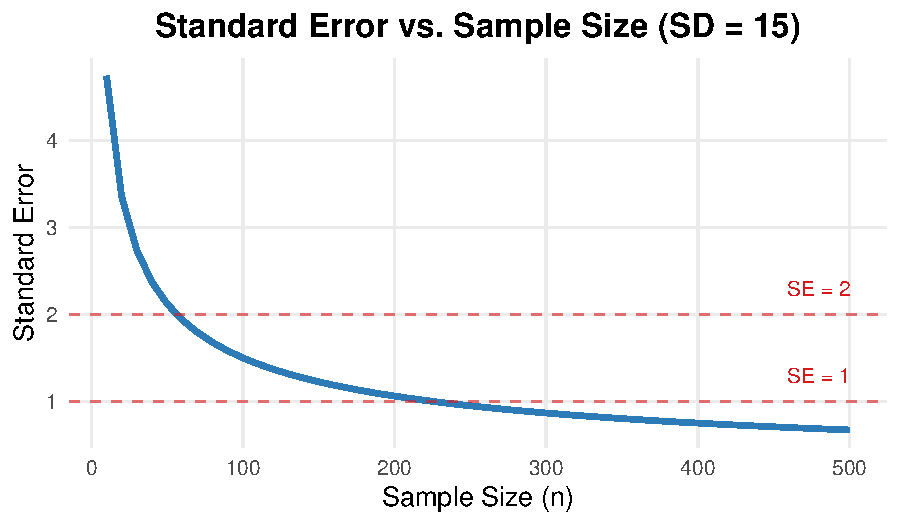
\includegraphics[keepaspectratio]{chapter04_estimation_files/figure-pdf/fig-se-1.pdf}}

}

\caption{\label{fig-se}As sample size increases, the standard error
decreases and estimates become more precise}

\end{figure}%

\begin{center}\rule{0.5\linewidth}{0.5pt}\end{center}

\bookmarksetup{startatroot}

\chapter{Confidence Interval for a
Mean}\label{confidence-interval-for-a-mean}

\section{When the Population SD Is Known
(Z-interval)}\label{when-the-population-sd-is-known-z-interval}

If the population standard deviation \(\sigma\) is known and either (a)
the population is normal, or (b) the sample size is large
(\(n \geq 30\)), we use the \textbf{Z-interval}:

\[\bar{x} \pm z_{\alpha/2} \cdot \frac{\sigma}{\sqrt{n}}\]

The \textbf{critical value} \(z_{\alpha/2}\) depends on the confidence
level:

\begin{Shaded}
\begin{Highlighting}[]
\NormalTok{crit }\OtherTok{\textless{}{-}} \FunctionTok{data.frame}\NormalTok{(}
  \StringTok{\textasciigrave{}}\AttributeTok{Confidence Level}\StringTok{\textasciigrave{}} \OtherTok{=} \FunctionTok{c}\NormalTok{(}\StringTok{"90\%"}\NormalTok{, }\StringTok{"95\%"}\NormalTok{, }\StringTok{"99\%"}\NormalTok{),}
  \StringTok{\textasciigrave{}}\AttributeTok{α}\StringTok{\textasciigrave{}} \OtherTok{=} \FunctionTok{c}\NormalTok{(}\StringTok{"0.10"}\NormalTok{, }\StringTok{"0.05"}\NormalTok{, }\StringTok{"0.01"}\NormalTok{),}
  \StringTok{\textasciigrave{}}\AttributeTok{α/2}\StringTok{\textasciigrave{}} \OtherTok{=} \FunctionTok{c}\NormalTok{(}\StringTok{"0.05"}\NormalTok{, }\StringTok{"0.025"}\NormalTok{, }\StringTok{"0.005"}\NormalTok{),}
  \StringTok{\textasciigrave{}}\AttributeTok{z(α/2)}\StringTok{\textasciigrave{}} \OtherTok{=} \FunctionTok{c}\NormalTok{(}\StringTok{"1.645"}\NormalTok{, }\StringTok{"1.960"}\NormalTok{, }\StringTok{"2.576"}\NormalTok{)}
\NormalTok{)}

\FunctionTok{kable}\NormalTok{(crit,}
      \AttributeTok{col.names =} \FunctionTok{c}\NormalTok{(}\StringTok{"Confidence Level"}\NormalTok{, }\StringTok{"α"}\NormalTok{, }\StringTok{"α/2"}\NormalTok{, }\StringTok{"z(α/2)"}\NormalTok{),}
      \AttributeTok{align =} \FunctionTok{c}\NormalTok{(}\StringTok{"c"}\NormalTok{,}\StringTok{"c"}\NormalTok{,}\StringTok{"c"}\NormalTok{,}\StringTok{"c"}\NormalTok{)) }\SpecialCharTok{|\textgreater{}}
  \FunctionTok{kable\_styling}\NormalTok{(}\AttributeTok{bootstrap\_options =} \FunctionTok{c}\NormalTok{(}\StringTok{"striped"}\NormalTok{,}\StringTok{"hover"}\NormalTok{,}\StringTok{"bordered"}\NormalTok{),}
                \AttributeTok{full\_width =} \ConstantTok{FALSE}\NormalTok{, }\AttributeTok{font\_size =} \DecValTok{13}\NormalTok{) }\SpecialCharTok{|\textgreater{}}
  \FunctionTok{column\_spec}\NormalTok{(}\DecValTok{1}\NormalTok{, }\AttributeTok{bold =} \ConstantTok{TRUE}\NormalTok{, }\AttributeTok{color =} \StringTok{"\#2c7bb6"}\NormalTok{) }\SpecialCharTok{|\textgreater{}}
  \FunctionTok{row\_spec}\NormalTok{(}\DecValTok{2}\NormalTok{, }\AttributeTok{background =} \StringTok{"\#eaf4fb"}\NormalTok{)}
\end{Highlighting}
\end{Shaded}

\begingroup\fontsize{13}{15}\selectfont

\begin{longtable}[t]{>{}cccc}

\caption{\label{tbl-z-critical}Critical Values for Common Confidence
Levels}

\tabularnewline

\toprule
Confidence Level & α & α/2 & z(α/2)\\
\midrule
\textcolor[HTML]{2c7bb6}{\textbf{90\%}} & 0.10 & 0.05 & 1.645\\
\cellcolor[HTML]{eaf4fb}{\textcolor[HTML]{2c7bb6}{\textbf{95\%}}} & \cellcolor[HTML]{eaf4fb}{0.05} & \cellcolor[HTML]{eaf4fb}{0.025} & \cellcolor[HTML]{eaf4fb}{1.960}\\
\textcolor[HTML]{2c7bb6}{\textbf{99\%}} & 0.01 & 0.005 & 2.576\\
\bottomrule

\end{longtable}

\endgroup{}

\begin{tcolorbox}[enhanced jigsaw, arc=.35mm, bottomrule=.15mm, bottomtitle=1mm, breakable, colback=white, colbacktitle=quarto-callout-tip-color!10!white, colframe=quarto-callout-tip-color-frame, coltitle=black, left=2mm, leftrule=.75mm, opacityback=0, opacitybacktitle=0.6, rightrule=.15mm, title={💡 The Most Used Value}, titlerule=0mm, toprule=.15mm, toptitle=1mm]

In health research, the 95\% CI with \(z_{0.025} = 1.96\) is by far the
most commonly reported. You will see it in almost every clinical paper.

\end{tcolorbox}

\begin{center}\rule{0.5\linewidth}{0.5pt}\end{center}

\section{When the Population SD Is Unknown
(t-interval)}\label{when-the-population-sd-is-unknown-t-interval}

In practice, \(\sigma\) is almost never known. When we use the sample SD
\(s\) as an estimate, we must use the \textbf{t-distribution} instead of
the Z-distribution:

\[\bar{x} \pm t_{\alpha/2,\, n-1} \cdot \frac{s}{\sqrt{n}}\]

Where \(t_{\alpha/2,\, n-1}\) is the critical value from the
\textbf{t-distribution} with \(n - 1\) \textbf{degrees of freedom (df)}.

\subsection{The t-Distribution}\label{the-t-distribution}

The t-distribution is similar to the standard normal distribution but
has \textbf{heavier tails} --- reflecting the extra uncertainty from
estimating \(\sigma\) with \(s\). As \(n\) increases, the t-distribution
approaches the Z-distribution.

\begin{Shaded}
\begin{Highlighting}[]
\NormalTok{x }\OtherTok{\textless{}{-}} \FunctionTok{seq}\NormalTok{(}\SpecialCharTok{{-}}\DecValTok{4}\NormalTok{, }\DecValTok{4}\NormalTok{, }\AttributeTok{length =} \DecValTok{500}\NormalTok{)}
\NormalTok{df\_plot }\OtherTok{\textless{}{-}} \FunctionTok{data.frame}\NormalTok{(}
  \AttributeTok{x =} \FunctionTok{rep}\NormalTok{(x, }\DecValTok{4}\NormalTok{),}
  \AttributeTok{y =} \FunctionTok{c}\NormalTok{(}\FunctionTok{dnorm}\NormalTok{(x),}
        \FunctionTok{dt}\NormalTok{(x, }\AttributeTok{df =} \DecValTok{3}\NormalTok{),}
        \FunctionTok{dt}\NormalTok{(x, }\AttributeTok{df =} \DecValTok{10}\NormalTok{),}
        \FunctionTok{dt}\NormalTok{(x, }\AttributeTok{df =} \DecValTok{30}\NormalTok{)),}
  \AttributeTok{dist =} \FunctionTok{rep}\NormalTok{(}\FunctionTok{c}\NormalTok{(}\StringTok{"Z (normal)"}\NormalTok{, }\StringTok{"t (df=3)"}\NormalTok{, }\StringTok{"t (df=10)"}\NormalTok{, }\StringTok{"t (df=30)"}\NormalTok{), }\AttributeTok{each =} \DecValTok{500}\NormalTok{)}
\NormalTok{)}

\NormalTok{df\_plot}\SpecialCharTok{$}\NormalTok{dist }\OtherTok{\textless{}{-}} \FunctionTok{factor}\NormalTok{(df\_plot}\SpecialCharTok{$}\NormalTok{dist,}
                       \AttributeTok{levels =} \FunctionTok{c}\NormalTok{(}\StringTok{"t (df=3)"}\NormalTok{,}\StringTok{"t (df=10)"}\NormalTok{,}\StringTok{"t (df=30)"}\NormalTok{,}\StringTok{"Z (normal)"}\NormalTok{))}

\FunctionTok{ggplot}\NormalTok{(df\_plot, }\FunctionTok{aes}\NormalTok{(}\AttributeTok{x =}\NormalTok{ x, }\AttributeTok{y =}\NormalTok{ y, }\AttributeTok{color =}\NormalTok{ dist, }\AttributeTok{linetype =}\NormalTok{ dist)) }\SpecialCharTok{+}
  \FunctionTok{geom\_line}\NormalTok{(}\AttributeTok{linewidth =} \DecValTok{1}\NormalTok{) }\SpecialCharTok{+}
  \FunctionTok{scale\_color\_manual}\NormalTok{(}\AttributeTok{values =} \FunctionTok{c}\NormalTok{(}\StringTok{"\#d7191c"}\NormalTok{,}\StringTok{"\#fdae61"}\NormalTok{,}\StringTok{"\#abd9e9"}\NormalTok{,}\StringTok{"\#2c7bb6"}\NormalTok{)) }\SpecialCharTok{+}
  \FunctionTok{scale\_linetype\_manual}\NormalTok{(}\AttributeTok{values =} \FunctionTok{c}\NormalTok{(}\StringTok{"dashed"}\NormalTok{,}\StringTok{"dashed"}\NormalTok{,}\StringTok{"dashed"}\NormalTok{,}\StringTok{"solid"}\NormalTok{)) }\SpecialCharTok{+}
  \FunctionTok{labs}\NormalTok{(}\AttributeTok{x =} \StringTok{"Value"}\NormalTok{, }\AttributeTok{y =} \StringTok{"Density"}\NormalTok{, }\AttributeTok{color =} \StringTok{"Distribution"}\NormalTok{, }\AttributeTok{linetype =} \StringTok{"Distribution"}\NormalTok{) }\SpecialCharTok{+}
  \FunctionTok{theme\_minimal}\NormalTok{(}\AttributeTok{base\_size =} \DecValTok{13}\NormalTok{) }\SpecialCharTok{+}
  \FunctionTok{theme}\NormalTok{(}\AttributeTok{legend.position =} \StringTok{"right"}\NormalTok{,}
        \AttributeTok{panel.grid.minor =} \FunctionTok{element\_blank}\NormalTok{())}
\end{Highlighting}
\end{Shaded}

\begin{figure}[H]

\centering{

\pandocbounded{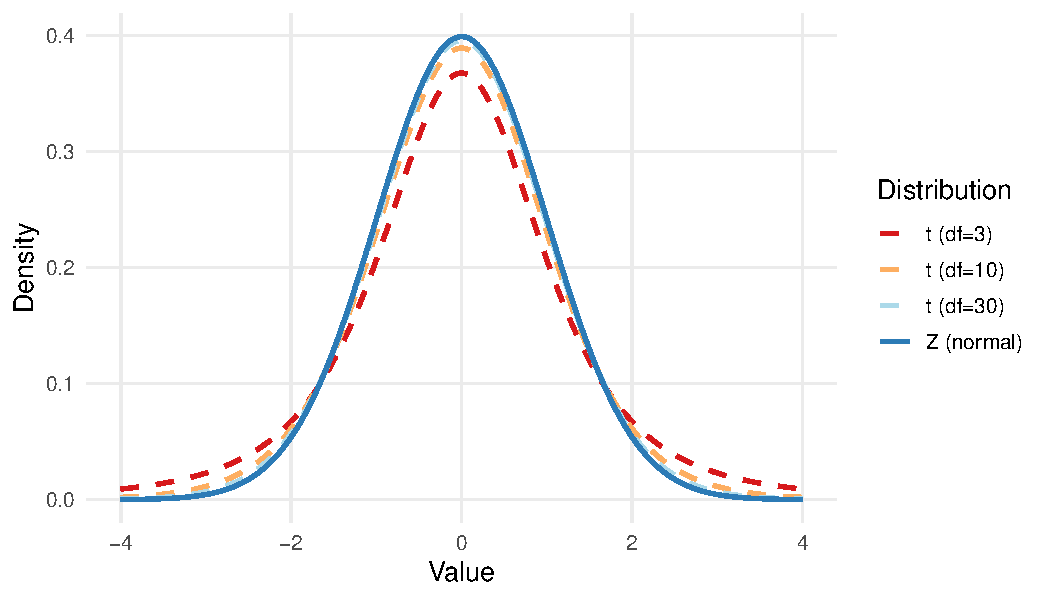
\includegraphics[keepaspectratio]{chapter04_estimation_files/figure-pdf/fig-t-dist-1.pdf}}

}

\caption{\label{fig-t-dist}t-distributions with different degrees of
freedom compared to Z}

\end{figure}%

\subsection{t Critical Values}\label{t-critical-values}

\begin{Shaded}
\begin{Highlighting}[]
\NormalTok{df\_vals }\OtherTok{\textless{}{-}} \FunctionTok{c}\NormalTok{(}\DecValTok{5}\NormalTok{, }\DecValTok{10}\NormalTok{, }\DecValTok{15}\NormalTok{, }\DecValTok{20}\NormalTok{, }\DecValTok{25}\NormalTok{, }\DecValTok{30}\NormalTok{, }\DecValTok{40}\NormalTok{, }\DecValTok{60}\NormalTok{, }\DecValTok{120}\NormalTok{, }\ConstantTok{Inf}\NormalTok{)}
\NormalTok{t\_vals  }\OtherTok{\textless{}{-}} \FunctionTok{qt}\NormalTok{(}\FloatTok{0.975}\NormalTok{, }\AttributeTok{df =}\NormalTok{ df\_vals)}
\NormalTok{t\_vals[}\FunctionTok{length}\NormalTok{(t\_vals)] }\OtherTok{\textless{}{-}} \FloatTok{1.960}

\NormalTok{t\_tab }\OtherTok{\textless{}{-}} \FunctionTok{data.frame}\NormalTok{(}
  \AttributeTok{df =} \FunctionTok{c}\NormalTok{(}\FunctionTok{as.character}\NormalTok{(df\_vals[}\SpecialCharTok{{-}}\FunctionTok{length}\NormalTok{(df\_vals)]), }\StringTok{"∞ (Z)"}\NormalTok{),}
  \AttributeTok{t  =} \FunctionTok{round}\NormalTok{(t\_vals, }\DecValTok{3}\NormalTok{)}
\NormalTok{)}

\FunctionTok{kable}\NormalTok{(t\_tab, }\AttributeTok{col.names =} \FunctionTok{c}\NormalTok{(}\StringTok{"Degrees of Freedom (df = n−1)"}\NormalTok{, }\StringTok{"t(0.025, df)"}\NormalTok{),}
      \AttributeTok{align =} \FunctionTok{c}\NormalTok{(}\StringTok{"c"}\NormalTok{,}\StringTok{"c"}\NormalTok{)) }\SpecialCharTok{|\textgreater{}}
  \FunctionTok{kable\_styling}\NormalTok{(}\AttributeTok{bootstrap\_options =} \FunctionTok{c}\NormalTok{(}\StringTok{"striped"}\NormalTok{,}\StringTok{"hover"}\NormalTok{,}\StringTok{"bordered"}\NormalTok{),}
                \AttributeTok{full\_width =} \ConstantTok{FALSE}\NormalTok{, }\AttributeTok{font\_size =} \DecValTok{13}\NormalTok{) }\SpecialCharTok{|\textgreater{}}
  \FunctionTok{column\_spec}\NormalTok{(}\DecValTok{1}\NormalTok{, }\AttributeTok{bold =} \ConstantTok{TRUE}\NormalTok{, }\AttributeTok{color =} \StringTok{"\#2c7bb6"}\NormalTok{) }\SpecialCharTok{|\textgreater{}}
  \FunctionTok{row\_spec}\NormalTok{(}\DecValTok{10}\NormalTok{, }\AttributeTok{background =} \StringTok{"\#eaf4fb"}\NormalTok{, }\AttributeTok{bold =} \ConstantTok{TRUE}\NormalTok{)}
\end{Highlighting}
\end{Shaded}

\begingroup\fontsize{13}{15}\selectfont

\begin{longtable}[t]{>{}cc}

\caption{\label{tbl-t-critical}Selected t Critical Values (95\% CI,
two-tailed: α/2 = 0.025)}

\tabularnewline

\toprule
Degrees of Freedom (df = n−1) & t(0.025, df)\\
\midrule
\textcolor[HTML]{2c7bb6}{\textbf{5}} & 2.571\\
\textcolor[HTML]{2c7bb6}{\textbf{10}} & 2.228\\
\textcolor[HTML]{2c7bb6}{\textbf{15}} & 2.131\\
\textcolor[HTML]{2c7bb6}{\textbf{20}} & 2.086\\
\textcolor[HTML]{2c7bb6}{\textbf{25}} & 2.060\\
\addlinespace
\textcolor[HTML]{2c7bb6}{\textbf{30}} & 2.042\\
\textcolor[HTML]{2c7bb6}{\textbf{40}} & 2.021\\
\textcolor[HTML]{2c7bb6}{\textbf{60}} & 2.000\\
\textcolor[HTML]{2c7bb6}{\textbf{120}} & 1.980\\
\cellcolor[HTML]{eaf4fb}{\textbf{\textcolor[HTML]{2c7bb6}{\textbf{∞ (Z)}}}} & \cellcolor[HTML]{eaf4fb}{\textbf{1.960}}\\
\bottomrule

\end{longtable}

\endgroup{}

As df increases, the t critical value converges to \textbf{1.960} (the Z
value). For \(n \geq 30\), the difference is small and Z is often used
as an approximation.

\begin{center}\rule{0.5\linewidth}{0.5pt}\end{center}

\bookmarksetup{startatroot}

\chapter{Confidence Interval for a
Proportion}\label{confidence-interval-for-a-proportion}

When the outcome of interest is a \textbf{proportion} (e.g., prevalence
of a disease, percentage of patients who respond to treatment), we use:

\[\hat{p} \pm z_{\alpha/2} \cdot \sqrt{\frac{\hat{p}(1-\hat{p})}{n}}\]

Where \(\hat{p} = \dfrac{x}{n}\) is the sample proportion (\(x\) =
number with the characteristic, \(n\) = total sample size).

\begin{tcolorbox}[enhanced jigsaw, arc=.35mm, bottomrule=.15mm, bottomtitle=1mm, breakable, colback=white, colbacktitle=quarto-callout-warning-color!10!white, colframe=quarto-callout-warning-color-frame, coltitle=black, left=2mm, leftrule=.75mm, opacityback=0, opacitybacktitle=0.6, rightrule=.15mm, title={⚠️ When Is This Formula Valid?}, titlerule=0mm, toprule=.15mm, toptitle=1mm]

This formula requires a \textbf{sufficiently large sample}. A common
rule of thumb is:

\[n\hat{p} \geq 5 \quad \text{and} \quad n(1-\hat{p}) \geq 5\]

If this condition is not met, special methods are needed (not covered in
this course).

\end{tcolorbox}

\begin{center}\rule{0.5\linewidth}{0.5pt}\end{center}

\bookmarksetup{startatroot}

\chapter{Interpreting a Confidence
Interval}\label{interpreting-a-confidence-interval}

\begin{tcolorbox}[enhanced jigsaw, arc=.35mm, bottomrule=.15mm, bottomtitle=1mm, breakable, colback=white, colbacktitle=quarto-callout-important-color!10!white, colframe=quarto-callout-important-color-frame, coltitle=black, left=2mm, leftrule=.75mm, opacityback=0, opacitybacktitle=0.6, rightrule=.15mm, title={✅ Correct Interpretation}, titlerule=0mm, toprule=.15mm, toptitle=1mm]

\begin{quote}
\emph{``We are 95\% confident that the true population mean lies between
{[}lower bound{]} and {[}upper bound{]}.''}
\end{quote}

\textbf{What this means:} If we repeated the sampling process many
times, 95\% of the resulting confidence intervals would contain the true
parameter.

\textbf{What this does NOT mean:} There is NOT a 95\% probability that
the true parameter lies in this specific interval --- the true parameter
is fixed; it either is or is not in the interval.

\end{tcolorbox}

\begin{Shaded}
\begin{Highlighting}[]
\FunctionTok{set.seed}\NormalTok{(}\DecValTok{42}\NormalTok{)}
\NormalTok{true\_mu }\OtherTok{\textless{}{-}} \DecValTok{130}
\NormalTok{sigma    }\OtherTok{\textless{}{-}} \DecValTok{15}
\NormalTok{n        }\OtherTok{\textless{}{-}} \DecValTok{40}
\NormalTok{n\_sims   }\OtherTok{\textless{}{-}} \DecValTok{50}

\NormalTok{sims }\OtherTok{\textless{}{-}} \FunctionTok{replicate}\NormalTok{(n\_sims, \{}
\NormalTok{  x    }\OtherTok{\textless{}{-}} \FunctionTok{rnorm}\NormalTok{(n, }\AttributeTok{mean =}\NormalTok{ true\_mu, }\AttributeTok{sd =}\NormalTok{ sigma)}
\NormalTok{  xbar }\OtherTok{\textless{}{-}} \FunctionTok{mean}\NormalTok{(x)}
\NormalTok{  se   }\OtherTok{\textless{}{-}} \FunctionTok{sd}\NormalTok{(x) }\SpecialCharTok{/} \FunctionTok{sqrt}\NormalTok{(n)}
  \FunctionTok{c}\NormalTok{(xbar, xbar }\SpecialCharTok{{-}} \FloatTok{1.96}\SpecialCharTok{*}\NormalTok{se, xbar }\SpecialCharTok{+} \FloatTok{1.96}\SpecialCharTok{*}\NormalTok{se)}
\NormalTok{\})}

\NormalTok{ci\_df }\OtherTok{\textless{}{-}} \FunctionTok{data.frame}\NormalTok{(}
  \AttributeTok{sim   =} \DecValTok{1}\SpecialCharTok{:}\NormalTok{n\_sims,}
  \AttributeTok{mean  =}\NormalTok{ sims[}\DecValTok{1}\NormalTok{,],}
  \AttributeTok{lower =}\NormalTok{ sims[}\DecValTok{2}\NormalTok{,],}
  \AttributeTok{upper =}\NormalTok{ sims[}\DecValTok{3}\NormalTok{,],}
  \AttributeTok{contains =}\NormalTok{ sims[}\DecValTok{2}\NormalTok{,] }\SpecialCharTok{\textless{}=}\NormalTok{ true\_mu }\SpecialCharTok{\&}\NormalTok{ sims[}\DecValTok{3}\NormalTok{,] }\SpecialCharTok{\textgreater{}=}\NormalTok{ true\_mu}
\NormalTok{)}

\FunctionTok{ggplot}\NormalTok{(ci\_df, }\FunctionTok{aes}\NormalTok{(}\AttributeTok{y =}\NormalTok{ sim, }\AttributeTok{color =}\NormalTok{ contains)) }\SpecialCharTok{+}
  \FunctionTok{geom\_segment}\NormalTok{(}\FunctionTok{aes}\NormalTok{(}\AttributeTok{x =}\NormalTok{ lower, }\AttributeTok{xend =}\NormalTok{ upper, }\AttributeTok{yend =}\NormalTok{ sim), }\AttributeTok{linewidth =} \FloatTok{0.8}\NormalTok{) }\SpecialCharTok{+}
  \FunctionTok{geom\_point}\NormalTok{(}\FunctionTok{aes}\NormalTok{(}\AttributeTok{x =}\NormalTok{ mean), }\AttributeTok{size =} \FloatTok{1.5}\NormalTok{) }\SpecialCharTok{+}
  \FunctionTok{geom\_vline}\NormalTok{(}\AttributeTok{xintercept =}\NormalTok{ true\_mu, }\AttributeTok{color =} \StringTok{"black"}\NormalTok{,}
             \AttributeTok{linetype =} \StringTok{"dashed"}\NormalTok{, }\AttributeTok{linewidth =} \DecValTok{1}\NormalTok{) }\SpecialCharTok{+}
  \FunctionTok{scale\_color\_manual}\NormalTok{(}\AttributeTok{values =} \FunctionTok{c}\NormalTok{(}\StringTok{"TRUE"} \OtherTok{=} \StringTok{"\#1a9641"}\NormalTok{, }\StringTok{"FALSE"} \OtherTok{=} \StringTok{"\#d7191c"}\NormalTok{),}
                     \AttributeTok{labels =} \FunctionTok{c}\NormalTok{(}\StringTok{"TRUE"} \OtherTok{=} \StringTok{"Contains μ"}\NormalTok{, }\StringTok{"FALSE"} \OtherTok{=} \StringTok{"Does not contain μ"}\NormalTok{),}
                     \AttributeTok{name =} \StringTok{""}\NormalTok{) }\SpecialCharTok{+}
  \FunctionTok{annotate}\NormalTok{(}\StringTok{"text"}\NormalTok{, }\AttributeTok{x =}\NormalTok{ true\_mu }\SpecialCharTok{+} \FloatTok{0.5}\NormalTok{, }\AttributeTok{y =} \DecValTok{52}\NormalTok{,}
           \AttributeTok{label =} \StringTok{"True μ = 130"}\NormalTok{, }\AttributeTok{hjust =} \DecValTok{0}\NormalTok{, }\AttributeTok{size =} \FloatTok{3.5}\NormalTok{) }\SpecialCharTok{+}
  \FunctionTok{labs}\NormalTok{(}\AttributeTok{x =} \StringTok{"Value"}\NormalTok{, }\AttributeTok{y =} \StringTok{"Sample Number"}\NormalTok{) }\SpecialCharTok{+}
  \FunctionTok{theme\_minimal}\NormalTok{(}\AttributeTok{base\_size =} \DecValTok{12}\NormalTok{) }\SpecialCharTok{+}
  \FunctionTok{theme}\NormalTok{(}\AttributeTok{legend.position =} \StringTok{"bottom"}\NormalTok{,}
        \AttributeTok{panel.grid.minor =} \FunctionTok{element\_blank}\NormalTok{())}
\end{Highlighting}
\end{Shaded}

\begin{figure}[H]

\centering{

\pandocbounded{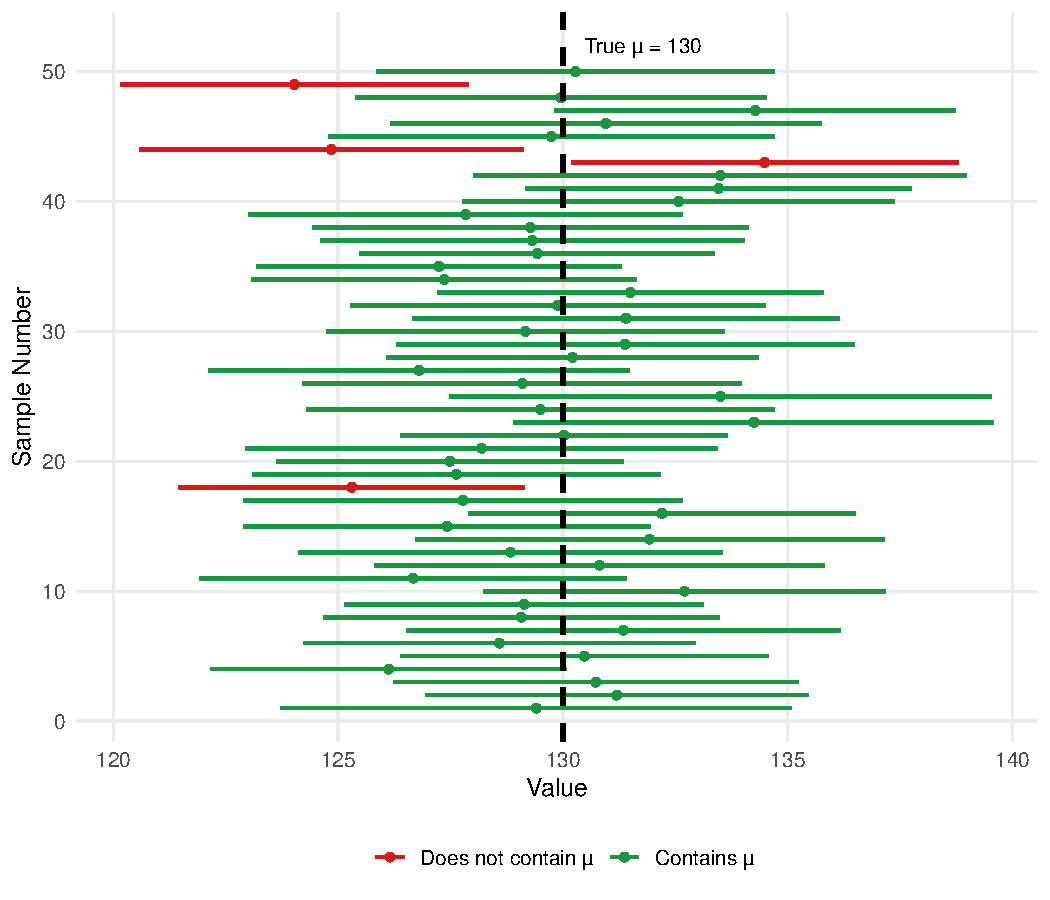
\includegraphics[keepaspectratio]{chapter04_estimation_files/figure-pdf/fig-ci-simulation-1.pdf}}

}

\caption{\label{fig-ci-simulation}Simulation: 50 confidence intervals
from repeated samples. Green intervals contain the true mean (μ = 130);
red ones do not.}

\end{figure}%

The figure above shows 50 confidence intervals from 50 different samples
of the same population. Most (≈95\%) contain the true mean; a few do not
--- this is expected and not an error.

\begin{center}\rule{0.5\linewidth}{0.5pt}\end{center}

\bookmarksetup{startatroot}

\chapter{Key Takeaways}\label{key-takeaways-3}

\begin{tcolorbox}[enhanced jigsaw, arc=.35mm, bottomrule=.15mm, bottomtitle=1mm, breakable, colback=white, colbacktitle=quarto-callout-note-color!10!white, colframe=quarto-callout-note-color-frame, coltitle=black, left=2mm, leftrule=.75mm, opacityback=0, opacitybacktitle=0.6, rightrule=.15mm, title={📝 Chapter 4 Summary}, titlerule=0mm, toprule=.15mm, toptitle=1mm]

\begin{enumerate}
\def\labelenumi{\arabic{enumi}.}
\item
  A \textbf{point estimate} gives a single best-guess value for a
  population parameter; an \textbf{interval estimate} gives a range of
  plausible values.
\item
  A \textbf{confidence interval (CI)} = Point estimate \(\pm\) Margin of
  error. The margin of error depends on the confidence level, the SE,
  and the critical value.
\item
  Use the \textbf{Z-interval} when \(\sigma\) is known or \(n \geq 30\);
  use the \textbf{t-interval} when \(\sigma\) is unknown and \(n\) is
  small, with \(df = n - 1\).
\item
  The \textbf{95\% CI} is the standard in health research, using
  \(z_{0.025} = 1.96\).
\item
  A wider CI means less precision; a larger sample size \(n\) always
  produces a narrower (more precise) CI.
\item
  The correct interpretation: \emph{``We are 95\% confident the true
  parameter lies within this interval''} --- not a probability statement
  about a fixed parameter.
\end{enumerate}

\end{tcolorbox}

\begin{center}\rule{0.5\linewidth}{0.5pt}\end{center}

\bookmarksetup{startatroot}

\chapter{Examples}\label{examples-3}

\section{Example 1: 95\% CI for a Mean (σ
unknown)}\label{example-1-95-ci-for-a-mean-ux3c3-unknown}

A study measured the fasting blood glucose (mg/dL) of a random sample of
\textbf{36 adults} and found:

\[\bar{x} = 105.4 \text{ mg/dL}, \qquad s = 18.6 \text{ mg/dL}\]

Construct a \textbf{95\% confidence interval} for the population mean
blood glucose.

\begin{tcolorbox}[enhanced jigsaw, arc=.35mm, bottomrule=.15mm, bottomtitle=1mm, breakable, colback=white, colbacktitle=quarto-callout-tip-color!10!white, colframe=quarto-callout-tip-color-frame, coltitle=black, left=2mm, leftrule=.75mm, opacityback=0, opacitybacktitle=0.6, rightrule=.15mm, title={✅ Solution}, titlerule=0mm, toprule=.15mm, toptitle=1mm]

\textbf{Given:} \(n = 36\), \(\bar{x} = 105.4\), \(s = 18.6\),
confidence level = 95\%

\textbf{Step 1 --- Standard Error:}
\[SE = \frac{s}{\sqrt{n}} = \frac{18.6}{\sqrt{36}} = \frac{18.6}{6} = 3.10\]

\textbf{Step 2 --- Critical value:}

\(df = n - 1 = 35\). From the t-table at \(\alpha/2 = 0.025\):
\(t_{0.025,\, 35} = 2.030\)

\emph{(Since \(n = 36 \geq 30\), we could also use \(z = 1.96\) as an
approximation.)}

\textbf{Step 3 --- Confidence Interval:}
\[105.4 \pm 2.030 \times 3.10 = 105.4 \pm 6.29\]

\[\textbf{95\% CI: } (99.1, \; 111.7) \text{ mg/dL}\]

\textbf{Interpretation:} We are 95\% confident that the true mean
fasting blood glucose of adults in this population is between
\textbf{99.1 and 111.7 mg/dL}.

\end{tcolorbox}

\begin{center}\rule{0.5\linewidth}{0.5pt}\end{center}

\section{Example 2: 95\% CI for a
Proportion}\label{example-2-95-ci-for-a-proportion}

In a survey of \textbf{200 adults}, \textbf{68 were found to have
hypertension}.

Construct a \textbf{95\% confidence interval} for the true prevalence of
hypertension in this population.

\begin{tcolorbox}[enhanced jigsaw, arc=.35mm, bottomrule=.15mm, bottomtitle=1mm, breakable, colback=white, colbacktitle=quarto-callout-tip-color!10!white, colframe=quarto-callout-tip-color-frame, coltitle=black, left=2mm, leftrule=.75mm, opacityback=0, opacitybacktitle=0.6, rightrule=.15mm, title={✅ Solution}, titlerule=0mm, toprule=.15mm, toptitle=1mm]

\textbf{Given:} \(n = 200\), \(x = 68\)

\textbf{Step 1 --- Sample proportion:}
\[\hat{p} = \frac{68}{200} = 0.34 \quad (34\%)\]

\textbf{Step 2 --- Check validity:}
\[n\hat{p} = 200 \times 0.34 = 68 \geq 5 \checkmark\]
\[n(1-\hat{p}) = 200 \times 0.66 = 132 \geq 5 \checkmark\]

\textbf{Step 3 --- Standard Error:}
\[SE = \sqrt{\frac{0.34 \times 0.66}{200}} = \sqrt{\frac{0.2244}{200}} = \sqrt{0.001122} = 0.0335\]

\textbf{Step 4 --- Confidence Interval} (using \(z_{0.025} = 1.96\)):
\[0.34 \pm 1.96 \times 0.0335 = 0.34 \pm 0.066\]

\[\textbf{95\% CI: } (0.274, \; 0.406) \quad \text{or} \quad (27.4\%, \; 40.6\%)\]

\textbf{Interpretation:} We are 95\% confident that the true prevalence
of hypertension in this population is between \textbf{27.4\% and
40.6\%}.

\end{tcolorbox}

\begin{center}\rule{0.5\linewidth}{0.5pt}\end{center}

\section{Example 3: Effect of Sample Size on CI
Width}\label{example-3-effect-of-sample-size-on-ci-width}

Using the same data as Example 1 (\(\bar{x} = 105.4\), \(s = 18.6\)),
compare the 95\% CI when \(n = 36\), \(n = 100\), and \(n = 400\).

\begin{tcolorbox}[enhanced jigsaw, arc=.35mm, bottomrule=.15mm, bottomtitle=1mm, breakable, colback=white, colbacktitle=quarto-callout-tip-color!10!white, colframe=quarto-callout-tip-color-frame, coltitle=black, left=2mm, leftrule=.75mm, opacityback=0, opacitybacktitle=0.6, rightrule=.15mm, title={✅ Solution}, titlerule=0mm, toprule=.15mm, toptitle=1mm]

\begin{Shaded}
\begin{Highlighting}[]
\NormalTok{ns   }\OtherTok{\textless{}{-}} \FunctionTok{c}\NormalTok{(}\DecValTok{36}\NormalTok{, }\DecValTok{100}\NormalTok{, }\DecValTok{400}\NormalTok{)}
\NormalTok{se   }\OtherTok{\textless{}{-}} \FloatTok{18.6} \SpecialCharTok{/} \FunctionTok{sqrt}\NormalTok{(ns)}
\NormalTok{z    }\OtherTok{\textless{}{-}} \FloatTok{1.96}
\NormalTok{me   }\OtherTok{\textless{}{-}}\NormalTok{ z }\SpecialCharTok{*}\NormalTok{ se}
\NormalTok{lo   }\OtherTok{\textless{}{-}} \FloatTok{105.4} \SpecialCharTok{{-}}\NormalTok{ me}
\NormalTok{hi   }\OtherTok{\textless{}{-}} \FloatTok{105.4} \SpecialCharTok{+}\NormalTok{ me}
\NormalTok{wid  }\OtherTok{\textless{}{-}}\NormalTok{ hi }\SpecialCharTok{{-}}\NormalTok{ lo}

\NormalTok{ci\_tab }\OtherTok{\textless{}{-}} \FunctionTok{data.frame}\NormalTok{(}
  \AttributeTok{n     =}\NormalTok{ ns,}
  \AttributeTok{SE    =} \FunctionTok{round}\NormalTok{(se, }\DecValTok{3}\NormalTok{),}
  \AttributeTok{ME    =} \FunctionTok{round}\NormalTok{(me, }\DecValTok{3}\NormalTok{),}
  \AttributeTok{Lower =} \FunctionTok{round}\NormalTok{(lo, }\DecValTok{2}\NormalTok{),}
  \AttributeTok{Upper =} \FunctionTok{round}\NormalTok{(hi, }\DecValTok{2}\NormalTok{),}
  \AttributeTok{Width =} \FunctionTok{round}\NormalTok{(wid, }\DecValTok{2}\NormalTok{)}
\NormalTok{)}

\FunctionTok{kable}\NormalTok{(ci\_tab,}
      \AttributeTok{col.names =} \FunctionTok{c}\NormalTok{(}\StringTok{"n"}\NormalTok{, }\StringTok{"SE"}\NormalTok{, }\StringTok{"Margin of Error"}\NormalTok{,}
                    \StringTok{"Lower Bound"}\NormalTok{, }\StringTok{"Upper Bound"}\NormalTok{, }\StringTok{"CI Width"}\NormalTok{),}
      \AttributeTok{align =} \FunctionTok{rep}\NormalTok{(}\StringTok{"c"}\NormalTok{, }\DecValTok{6}\NormalTok{)) }\SpecialCharTok{|\textgreater{}}
  \FunctionTok{kable\_styling}\NormalTok{(}\AttributeTok{bootstrap\_options =} \FunctionTok{c}\NormalTok{(}\StringTok{"striped"}\NormalTok{,}\StringTok{"hover"}\NormalTok{,}\StringTok{"bordered"}\NormalTok{),}
                \AttributeTok{full\_width =} \ConstantTok{FALSE}\NormalTok{, }\AttributeTok{font\_size =} \DecValTok{13}\NormalTok{) }\SpecialCharTok{|\textgreater{}}
  \FunctionTok{column\_spec}\NormalTok{(}\DecValTok{1}\NormalTok{, }\AttributeTok{bold =} \ConstantTok{TRUE}\NormalTok{, }\AttributeTok{color =} \StringTok{"\#2c7bb6"}\NormalTok{) }\SpecialCharTok{|\textgreater{}}
  \FunctionTok{column\_spec}\NormalTok{(}\DecValTok{6}\NormalTok{, }\AttributeTok{bold =} \ConstantTok{TRUE}\NormalTok{)}
\end{Highlighting}
\end{Shaded}

\begingroup\fontsize{13}{15}\selectfont

\begin{longtable}[t]{>{}ccccc>{}c}

\caption{\label{tbl-ci-width}Effect of Sample Size on CI Width (x̄ =
105.4, s = 18.6, 95\% CI)}

\tabularnewline

\toprule
n & SE & Margin of Error & Lower Bound & Upper Bound & CI Width\\
\midrule
\textcolor[HTML]{2c7bb6}{\textbf{36}} & 3.10 & 6.076 & 99.32 & 111.48 & \textbf{12.15}\\
\textcolor[HTML]{2c7bb6}{\textbf{100}} & 1.86 & 3.646 & 101.75 & 109.05 & \textbf{7.29}\\
\textcolor[HTML]{2c7bb6}{\textbf{400}} & 0.93 & 1.823 & 103.58 & 107.22 & \textbf{3.65}\\
\bottomrule

\end{longtable}

\endgroup{}

\textbf{Conclusion:} Quadrupling the sample size (from 100 to 400)
\textbf{halves} the CI width --- because SE depends on \(\sqrt{n}\), not
\(n\) directly. To halve the margin of error, you need to
\textbf{quadruple} the sample size.

\end{tcolorbox}

\begin{center}\rule{0.5\linewidth}{0.5pt}\end{center}

\bookmarksetup{startatroot}

\chapter{Exercises}\label{exercises-3}

\begin{tcolorbox}[enhanced jigsaw, arc=.35mm, bottomrule=.15mm, bottomtitle=1mm, breakable, colback=white, colbacktitle=quarto-callout-caution-color!10!white, colframe=quarto-callout-caution-color-frame, coltitle=black, left=2mm, leftrule=.75mm, opacityback=0, opacitybacktitle=0.6, rightrule=.15mm, title={✏️ Exercise 1}, titlerule=0mm, toprule=.15mm, toptitle=1mm]

A random sample of \textbf{25 patients} with chronic kidney disease had
their serum creatinine levels measured:

\[\bar{x} = 3.82 \text{ mg/dL}, \qquad s = 1.14 \text{ mg/dL}\]

\textbf{(a)} Calculate the standard error of the mean.

\textbf{(b)} Find the appropriate critical value for a 95\% CI.

\textbf{(c)} Construct the \textbf{95\% confidence interval} for the
population mean serum creatinine level.

\textbf{(d)} Interpret the confidence interval in plain language.

\end{tcolorbox}

\begin{tcolorbox}[enhanced jigsaw, arc=.35mm, bottomrule=.15mm, bottomtitle=1mm, breakable, colback=white, colbacktitle=quarto-callout-caution-color!10!white, colframe=quarto-callout-caution-color-frame, coltitle=black, left=2mm, leftrule=.75mm, opacityback=0, opacitybacktitle=0.6, rightrule=.15mm, title={✏️ Exercise 2}, titlerule=0mm, toprule=.15mm, toptitle=1mm]

A hospital records that \textbf{45 out of 180 patients} discharged last
month were readmitted within 30 days.

\textbf{(a)} Calculate the sample proportion of 30-day readmissions.

\textbf{(b)} Check whether the large-sample conditions are satisfied.

\textbf{(c)} Construct a \textbf{95\% confidence interval} for the true
30-day readmission rate.

\textbf{(d)} The hospital's target readmission rate is 20\%. Based on
the confidence interval, is there evidence that the true rate differs
from this target? Explain.

\end{tcolorbox}

\begin{tcolorbox}[enhanced jigsaw, arc=.35mm, bottomrule=.15mm, bottomtitle=1mm, breakable, colback=white, colbacktitle=quarto-callout-caution-color!10!white, colframe=quarto-callout-caution-color-frame, coltitle=black, left=2mm, leftrule=.75mm, opacityback=0, opacitybacktitle=0.6, rightrule=.15mm, title={✏️ Exercise 3}, titlerule=0mm, toprule=.15mm, toptitle=1mm]

A researcher wants to estimate the mean diastolic blood pressure (DBP)
of adults in a city. From a pilot study, the SD is estimated to be
\textbf{12 mmHg}.

The researcher wants a \textbf{95\% CI with a margin of error no greater
than 2 mmHg}.

Using the formula:
\[n = \left(\frac{z_{\alpha/2} \cdot \sigma}{E}\right)^2\]

where \(E\) is the desired margin of error, calculate the
\textbf{minimum sample size} required.

\end{tcolorbox}

\begin{center}\rule{0.5\linewidth}{0.5pt}\end{center}

\emph{End of Chapter 4}

\begin{center}\rule{0.5\linewidth}{0.5pt}\end{center}

\begin{tcolorbox}[enhanced jigsaw, arc=.35mm, bottomrule=.15mm, bottomtitle=1mm, breakable, colback=white, colbacktitle=quarto-callout-note-color!10!white, colframe=quarto-callout-note-color-frame, coltitle=black, left=2mm, leftrule=.75mm, opacityback=0, opacitybacktitle=0.6, rightrule=.15mm, title={📚 Coming Up Next}, titlerule=0mm, toprule=.15mm, toptitle=1mm]

\textbf{Chapter 5: Statistical Testing} --- Instead of estimating a
parameter, we will test specific claims about populations using
\textbf{hypothesis testing} --- one of the most powerful tools in health
research.

\end{tcolorbox}

\bookmarksetup{startatroot}

\chapter{Statistical Testing}\label{statistical-testing}

\begin{center}\rule{0.5\linewidth}{0.5pt}\end{center}

\bookmarksetup{startatroot}

\chapter*{Introduction}\label{introduction-4}
\addcontentsline{toc}{chapter}{Introduction}

\markboth{Introduction}{Introduction}

\begin{tcolorbox}[enhanced jigsaw, arc=.35mm, bottomrule=.15mm, bottomtitle=1mm, breakable, colback=white, colbacktitle=quarto-callout-note-color!10!white, colframe=quarto-callout-note-color-frame, coltitle=black, left=2mm, leftrule=.75mm, opacityback=0, opacitybacktitle=0.6, rightrule=.15mm, title={💡 Why Does This Matter?}, titlerule=0mm, toprule=.15mm, toptitle=1mm]

In health research, we constantly ask questions that require a decision:

\begin{itemize}
\tightlist
\item
  Does this new drug lower blood pressure \emph{more} than the standard
  treatment?
\item
  Is there a relationship between smoking and lung disease?
\item
  Do recovery times differ between two surgical techniques?
\end{itemize}

We cannot answer these questions simply by looking at sample means or
proportions --- random chance alone can create apparent differences
between groups. \textbf{Statistical testing} gives us a formal,
objective framework for deciding whether an observed difference is
likely to be real or simply due to chance.

This is the most widely used tool in health research, and understanding
it is essential for reading and interpreting scientific literature.

\end{tcolorbox}

\begin{center}\rule{0.5\linewidth}{0.5pt}\end{center}

\bookmarksetup{startatroot}

\chapter{Concept of Hypothesis
Testing}\label{concept-of-hypothesis-testing}

\section{The Logic of Hypothesis
Testing}\label{the-logic-of-hypothesis-testing}

Statistical testing works by assuming the opposite of what we want to
prove, then asking: \emph{``If nothing were really happening, how
surprising would our data be?''}

If the data would be very surprising under the assumption that nothing
is happening, we conclude that something probably \emph{is} happening.

\begin{center}\rule{0.5\linewidth}{0.5pt}\end{center}

\section{The Two Hypotheses}\label{the-two-hypotheses}

Every hypothesis test involves two competing statements:

\subsection{\texorpdfstring{Null Hypothesis
(\(H_0\))}{Null Hypothesis (H\_0)}}\label{null-hypothesis-h_0}

The \textbf{null hypothesis} states that there is \textbf{no effect, no
difference, or no relationship} in the population. It is the assumption
we start with and attempt to disprove.

\begin{quote}
\emph{Examples:} - The mean blood pressure is 120 mmHg.
(\(H_0: \mu = 120\)) - There is no difference in recovery time between
the two groups. (\(H_0: \mu_1 = \mu_2\)) - There is no association
between smoking status and disease. (\(H_0:\) no association)
\end{quote}

\subsection{\texorpdfstring{Alternative Hypothesis (\(H_1\) or
\(H_a\))}{Alternative Hypothesis (H\_1 or H\_a)}}\label{alternative-hypothesis-h_1-or-h_a}

The \textbf{alternative hypothesis} states that there \textbf{is} an
effect, difference, or relationship. This is usually what the researcher
believes or wants to demonstrate.

\begin{quote}
\emph{Examples:} - The mean blood pressure is not 120 mmHg.
(\(H_1: \mu \neq 120\)) - Recovery time differs between the two groups.
(\(H_1: \mu_1 \neq \mu_2\)) - There is an association between smoking
and disease. (\(H_1:\) association exists)
\end{quote}

\begin{center}\rule{0.5\linewidth}{0.5pt}\end{center}

\section{One-Tailed vs.~Two-Tailed
Tests}\label{one-tailed-vs.-two-tailed-tests}

The alternative hypothesis can be \textbf{directional} or
\textbf{non-directional}:

\begin{Shaded}
\begin{Highlighting}[]
\NormalTok{tails }\OtherTok{\textless{}{-}} \FunctionTok{data.frame}\NormalTok{(}
  \AttributeTok{Type =} \FunctionTok{c}\NormalTok{(}\StringTok{"Two{-}tailed"}\NormalTok{, }\StringTok{"One{-}tailed (right)"}\NormalTok{, }\StringTok{"One{-}tailed (left)"}\NormalTok{),}
  \StringTok{\textasciigrave{}}\AttributeTok{H₁}\StringTok{\textasciigrave{}} \OtherTok{=} \FunctionTok{c}\NormalTok{(}\StringTok{"μ ≠ μ₀  (different from)"}\NormalTok{, }\StringTok{"μ \textgreater{} μ₀  (greater than)"}\NormalTok{, }\StringTok{"μ \textless{} μ₀  (less than)"}\NormalTok{),}
  \StringTok{\textasciigrave{}}\AttributeTok{Use When}\StringTok{\textasciigrave{}} \OtherTok{=} \FunctionTok{c}\NormalTok{(}
    \StringTok{"You want to detect a difference in either direction (most common)"}\NormalTok{,}
    \StringTok{"You specifically expect the value to be higher"}\NormalTok{,}
    \StringTok{"You specifically expect the value to be lower"}
\NormalTok{  )}
\NormalTok{)}

\FunctionTok{kable}\NormalTok{(tails, }\AttributeTok{col.names =} \FunctionTok{c}\NormalTok{(}\StringTok{"Test Type"}\NormalTok{, }\StringTok{"H₁"}\NormalTok{, }\StringTok{"Use When"}\NormalTok{),}
      \AttributeTok{align =} \FunctionTok{c}\NormalTok{(}\StringTok{"l"}\NormalTok{,}\StringTok{"l"}\NormalTok{,}\StringTok{"l"}\NormalTok{)) }\SpecialCharTok{|\textgreater{}}
  \FunctionTok{kable\_styling}\NormalTok{(}\AttributeTok{bootstrap\_options =} \FunctionTok{c}\NormalTok{(}\StringTok{"striped"}\NormalTok{,}\StringTok{"hover"}\NormalTok{,}\StringTok{"bordered"}\NormalTok{),}
                \AttributeTok{full\_width =} \ConstantTok{TRUE}\NormalTok{, }\AttributeTok{font\_size =} \DecValTok{13}\NormalTok{) }\SpecialCharTok{|\textgreater{}}
  \FunctionTok{column\_spec}\NormalTok{(}\DecValTok{1}\NormalTok{, }\AttributeTok{bold =} \ConstantTok{TRUE}\NormalTok{, }\AttributeTok{color =} \StringTok{"\#2c7bb6"}\NormalTok{) }\SpecialCharTok{|\textgreater{}}
  \FunctionTok{row\_spec}\NormalTok{(}\DecValTok{1}\NormalTok{, }\AttributeTok{background =} \StringTok{"\#eaf4fb"}\NormalTok{)}
\end{Highlighting}
\end{Shaded}

\begin{table}

\caption{\label{tbl-tails}One-tailed vs.~Two-tailed Tests}

\centering{

\begingroup\fontsize{13}{15}\selectfont

\begin{longtabu} to \linewidth {>{}l>{\raggedright}X>{\raggedright}X}
\toprule
Test Type & H₁ & Use When\\
\midrule
\cellcolor[HTML]{eaf4fb}{\textcolor[HTML]{2c7bb6}{\textbf{Two-tailed}}} & \cellcolor[HTML]{eaf4fb}{μ ≠ μ₀  (different from)} & \cellcolor[HTML]{eaf4fb}{You want to detect a difference in either direction (most common)}\\
\textcolor[HTML]{2c7bb6}{\textbf{One-tailed (right)}} & μ > μ₀  (greater than) & You specifically expect the value to be higher\\
\textcolor[HTML]{2c7bb6}{\textbf{One-tailed (left)}} & μ < μ₀  (less than) & You specifically expect the value to be lower\\
\bottomrule
\end{longtabu}
\endgroup{}

}

\end{table}%

\begin{tcolorbox}[enhanced jigsaw, arc=.35mm, bottomrule=.15mm, bottomtitle=1mm, breakable, colback=white, colbacktitle=quarto-callout-tip-color!10!white, colframe=quarto-callout-tip-color-frame, coltitle=black, left=2mm, leftrule=.75mm, opacityback=0, opacitybacktitle=0.6, rightrule=.15mm, title={💡 Practical Advice}, titlerule=0mm, toprule=.15mm, toptitle=1mm]

In most health research, use a \textbf{two-tailed test} unless you have
a strong, pre-specified reason to test in only one direction. Two-tailed
tests are more conservative and more widely accepted.

\end{tcolorbox}

\begin{center}\rule{0.5\linewidth}{0.5pt}\end{center}

\section{The p-value}\label{the-p-value}

The \textbf{p-value} is the probability of obtaining results \emph{at
least as extreme as those observed}, assuming the null hypothesis is
true.

\[p\text{-value} = P(\text{observed result or more extreme} \mid H_0 \text{ is true})\]

\begin{itemize}
\tightlist
\item
  A \textbf{small p-value} means the observed data would be very
  unlikely if \(H_0\) were true → evidence against \(H_0\)
\item
  A \textbf{large p-value} means the observed data are consistent with
  \(H_0\) → insufficient evidence to reject \(H_0\)
\end{itemize}

\begin{center}\rule{0.5\linewidth}{0.5pt}\end{center}

\section{The Significance Level (α)}\label{the-significance-level-ux3b1}

The \textbf{significance level} \(\alpha\) is the threshold we set in
advance for deciding whether the p-value is ``small enough'' to reject
\(H_0\).

The most common choice in health research is \(\alpha = 0.05\).

{\def\LTcaptype{none} % do not increment counter
\begin{longtable}[]{@{}
  >{\raggedright\arraybackslash}p{(\linewidth - 2\tabcolsep) * \real{0.5000}}
  >{\raggedright\arraybackslash}p{(\linewidth - 2\tabcolsep) * \real{0.5000}}@{}}
\toprule\noalign{}
\begin{minipage}[b]{\linewidth}\raggedright
Decision Rule
\end{minipage} & \begin{minipage}[b]{\linewidth}\raggedright
\end{minipage} \\
\midrule\noalign{}
\endhead
\bottomrule\noalign{}
\endlastfoot
If \(p\text{-value} \leq \alpha\) & \textbf{Reject \(H_0\)} --- result
is statistically significant \\
If \(p\text{-value} > \alpha\) & \textbf{Fail to reject \(H_0\)} ---
insufficient evidence \\
\end{longtable}
}

\begin{tcolorbox}[enhanced jigsaw, arc=.35mm, bottomrule=.15mm, bottomtitle=1mm, breakable, colback=white, colbacktitle=quarto-callout-warning-color!10!white, colframe=quarto-callout-warning-color-frame, coltitle=black, left=2mm, leftrule=.75mm, opacityback=0, opacitybacktitle=0.6, rightrule=.15mm, title={⚠️ Common Misinterpretations}, titlerule=0mm, toprule=.15mm, toptitle=1mm]

\textbf{``Failing to reject \(H_0\)'' is NOT the same as proving \(H_0\)
is true.} It simply means the data do not provide strong enough evidence
against it.

\textbf{``Statistically significant'' does NOT necessarily mean
clinically important.} With a very large sample, even a trivially small
difference can become statistically significant. Always consider the
practical meaning of results.

\end{tcolorbox}

\begin{center}\rule{0.5\linewidth}{0.5pt}\end{center}

\section{Type I and Type II Errors}\label{type-i-and-type-ii-errors}

When making a decision about \(H_0\), two types of errors are possible:

\begin{Shaded}
\begin{Highlighting}[]
\NormalTok{errors }\OtherTok{\textless{}{-}} \FunctionTok{data.frame}\NormalTok{(}
  \StringTok{\textasciigrave{}}\AttributeTok{ }\StringTok{\textasciigrave{}} \OtherTok{=} \FunctionTok{c}\NormalTok{(}\StringTok{"**Reject H₀**"}\NormalTok{, }\StringTok{"**Fail to reject H₀**"}\NormalTok{),}
  \StringTok{\textasciigrave{}}\AttributeTok{H₀ is actually TRUE}\StringTok{\textasciigrave{}} \OtherTok{=} \FunctionTok{c}\NormalTok{(}\StringTok{"❌ Type I Error (α)}\SpecialCharTok{\textbackslash{}n}\StringTok{(False Positive)"}\NormalTok{,}
                              \StringTok{"✅ Correct Decision"}\NormalTok{),}
  \StringTok{\textasciigrave{}}\AttributeTok{H₀ is actually FALSE}\StringTok{\textasciigrave{}} \OtherTok{=} \FunctionTok{c}\NormalTok{(}\StringTok{"✅ Correct Decision}\SpecialCharTok{\textbackslash{}n}\StringTok{(Power = 1 − β)"}\NormalTok{,}
                               \StringTok{"❌ Type II Error (β)}\SpecialCharTok{\textbackslash{}n}\StringTok{(False Negative)"}\NormalTok{)}
\NormalTok{)}

\FunctionTok{kable}\NormalTok{(errors, }\AttributeTok{col.names =} \FunctionTok{c}\NormalTok{(}\StringTok{"Our Decision"}\NormalTok{, }\StringTok{"H₀ is TRUE"}\NormalTok{, }\StringTok{"H₀ is FALSE"}\NormalTok{),}
      \AttributeTok{align =} \FunctionTok{c}\NormalTok{(}\StringTok{"l"}\NormalTok{,}\StringTok{"c"}\NormalTok{,}\StringTok{"c"}\NormalTok{), }\AttributeTok{escape =} \ConstantTok{FALSE}\NormalTok{) }\SpecialCharTok{|\textgreater{}}
  \FunctionTok{kable\_styling}\NormalTok{(}\AttributeTok{bootstrap\_options =} \FunctionTok{c}\NormalTok{(}\StringTok{"bordered"}\NormalTok{),}
                \AttributeTok{full\_width =} \ConstantTok{TRUE}\NormalTok{, }\AttributeTok{font\_size =} \DecValTok{13}\NormalTok{) }\SpecialCharTok{|\textgreater{}}
  \FunctionTok{column\_spec}\NormalTok{(}\DecValTok{1}\NormalTok{, }\AttributeTok{bold =} \ConstantTok{TRUE}\NormalTok{) }\SpecialCharTok{|\textgreater{}}
  \FunctionTok{column\_spec}\NormalTok{(}\DecValTok{2}\NormalTok{, }\AttributeTok{background =} \FunctionTok{c}\NormalTok{(}\StringTok{"\#fde0d9"}\NormalTok{,}\StringTok{"\#d9f0d3"}\NormalTok{)) }\SpecialCharTok{|\textgreater{}}
  \FunctionTok{column\_spec}\NormalTok{(}\DecValTok{3}\NormalTok{, }\AttributeTok{background =} \FunctionTok{c}\NormalTok{(}\StringTok{"\#d9f0d3"}\NormalTok{,}\StringTok{"\#fde0d9"}\NormalTok{))}
\end{Highlighting}
\end{Shaded}

\begin{table}

\caption{\label{tbl-errors}Type I and Type II Errors in Hypothesis
Testing}

\centering{

\begingroup\fontsize{13}{15}\selectfont

\begin{longtabu} to \linewidth {>{}l>{}c>{}c}
\toprule
Our Decision & H₀ is TRUE & H₀ is FALSE\\
\midrule
**Reject H₀** & ❌ Type I Error (α)
(False Positive) & ✅ Correct Decision
\textbf{(Power = 1 − β)} & \cellcolor[HTML]{fde0d9}{NA} & \cellcolor[HTML]{d9f0d3}{NA}\\
**Fail to reject H₀** & ✅ Correct Decision         | & ❌ Type II Error (β)
\textbf{(False Negative) |} & \cellcolor[HTML]{d9f0d3}{NA} & \cellcolor[HTML]{fde0d9}{NA}\\
\bottomrule
\end{longtabu}
\endgroup{}

}

\end{table}%

\begin{itemize}
\tightlist
\item
  \textbf{Type I error (α):} Concluding there is an effect when there is
  none (\emph{false positive}). Controlled by choosing α (usually 0.05).
\item
  \textbf{Type II error (β):} Missing a real effect (\emph{false
  negative}). The probability of correctly detecting a real effect is
  called \textbf{power} = \(1 - \beta\).
\end{itemize}

\begin{center}\rule{0.5\linewidth}{0.5pt}\end{center}

\section{General Steps in Hypothesis
Testing}\label{general-steps-in-hypothesis-testing}

\begin{tcolorbox}[enhanced jigsaw, arc=.35mm, bottomrule=.15mm, bottomtitle=1mm, breakable, colback=white, colbacktitle=quarto-callout-important-color!10!white, colframe=quarto-callout-important-color-frame, coltitle=black, left=2mm, leftrule=.75mm, opacityback=0, opacitybacktitle=0.6, rightrule=.15mm, title={📋 The 5-Step Framework}, titlerule=0mm, toprule=.15mm, toptitle=1mm]

\textbf{Step 1 --- State the hypotheses:} Write \(H_0\) and \(H_1\)
clearly.

\textbf{Step 2 --- Choose the significance level:} Usually
\(\alpha = 0.05\).

\textbf{Step 3 --- Select and compute the test statistic:} A number
calculated from the sample that measures how far the data are from what
\(H_0\) predicts.

\textbf{Step 4 --- Find the p-value:} The probability of getting a test
statistic this extreme if \(H_0\) is true.

\textbf{Step 5 --- Make a decision and interpret:} Compare p-value to α.
State your conclusion in the context of the problem.

\end{tcolorbox}

\begin{center}\rule{0.5\linewidth}{0.5pt}\end{center}

\bookmarksetup{startatroot}

\chapter{Statistical Testing on Categorical
Data}\label{statistical-testing-on-categorical-data}

\section{Chi-Square Test for Two Independent
Groups}\label{chi-square-test-for-two-independent-groups}

\subsection{When to Use}\label{when-to-use}

The \textbf{chi-square test of independence} is used when:

\begin{itemize}
\tightlist
\item
  The outcome variable is \textbf{categorical (nominal)}
\item
  We are comparing \textbf{two or more independent groups}
\item
  We want to test whether there is an \textbf{association} between two
  categorical variables
\end{itemize}

\subsection{The Contingency Table}\label{the-contingency-table}

Data are arranged in a \textbf{contingency table} (also called a
cross-tabulation):

\[\begin{array}{|l|c|c|c|}
\hline
& \textbf{Outcome: Yes} & \textbf{Outcome: No} & \textbf{Row Total} \\
\hline
\textbf{Group 1} & a & b & a+b \\
\textbf{Group 2} & c & d & c+d \\
\hline
\textbf{Column Total} & a+c & b+d & n \\
\hline
\end{array}\]

\subsection{The Test Statistic}\label{the-test-statistic}

\[\chi^2 = \sum \frac{(O - E)^2}{E}\]

Where: - \(O\) = observed frequency (actual count in each cell) - \(E\)
= expected frequency =
\(\dfrac{\text{Row total} \times \text{Column total}}{n}\)

The sum is taken over \textbf{all cells} in the table.

The test statistic follows a \textbf{chi-square distribution} with
\(df = (\text{rows} - 1) \times (\text{columns} - 1)\).

For a \(2 \times 2\) table: \(df = (2-1)(2-1) = 1\).

\begin{tcolorbox}[enhanced jigsaw, arc=.35mm, bottomrule=.15mm, bottomtitle=1mm, breakable, colback=white, colbacktitle=quarto-callout-warning-color!10!white, colframe=quarto-callout-warning-color-frame, coltitle=black, left=2mm, leftrule=.75mm, opacityback=0, opacitybacktitle=0.6, rightrule=.15mm, title={⚠️ Condition for Valid Chi-Square Test}, titlerule=0mm, toprule=.15mm, toptitle=1mm]

All \textbf{expected frequencies} must be \(\geq 5\). If this condition
is violated, use \textbf{Fisher's exact test} instead (available in
SPSS).

\end{tcolorbox}

\subsection{Chi-Square Critical
Values}\label{chi-square-critical-values}

\begin{Shaded}
\begin{Highlighting}[]
\NormalTok{df\_chi  }\OtherTok{\textless{}{-}} \DecValTok{1}\SpecialCharTok{:}\DecValTok{10}
\NormalTok{cv\_chi  }\OtherTok{\textless{}{-}} \FunctionTok{round}\NormalTok{(}\FunctionTok{qchisq}\NormalTok{(}\FloatTok{0.95}\NormalTok{, }\AttributeTok{df =}\NormalTok{ df\_chi), }\DecValTok{3}\NormalTok{)}

\NormalTok{chi\_tab }\OtherTok{\textless{}{-}} \FunctionTok{data.frame}\NormalTok{(}\AttributeTok{df =}\NormalTok{ df\_chi, }\AttributeTok{critical =}\NormalTok{ cv\_chi)}

\FunctionTok{kable}\NormalTok{(chi\_tab, }\AttributeTok{col.names =} \FunctionTok{c}\NormalTok{(}\StringTok{"Degrees of Freedom (df)"}\NormalTok{, }\StringTok{"χ² critical value (α = 0.05)"}\NormalTok{),}
      \AttributeTok{align =} \FunctionTok{c}\NormalTok{(}\StringTok{"c"}\NormalTok{,}\StringTok{"c"}\NormalTok{)) }\SpecialCharTok{|\textgreater{}}
  \FunctionTok{kable\_styling}\NormalTok{(}\AttributeTok{bootstrap\_options =} \FunctionTok{c}\NormalTok{(}\StringTok{"striped"}\NormalTok{,}\StringTok{"hover"}\NormalTok{,}\StringTok{"bordered"}\NormalTok{),}
                \AttributeTok{full\_width =} \ConstantTok{FALSE}\NormalTok{, }\AttributeTok{font\_size =} \DecValTok{13}\NormalTok{) }\SpecialCharTok{|\textgreater{}}
  \FunctionTok{column\_spec}\NormalTok{(}\DecValTok{1}\NormalTok{, }\AttributeTok{bold =} \ConstantTok{TRUE}\NormalTok{, }\AttributeTok{color =} \StringTok{"\#2c7bb6"}\NormalTok{) }\SpecialCharTok{|\textgreater{}}
  \FunctionTok{row\_spec}\NormalTok{(}\DecValTok{1}\NormalTok{, }\AttributeTok{background =} \StringTok{"\#eaf4fb"}\NormalTok{)}
\end{Highlighting}
\end{Shaded}

\begingroup\fontsize{13}{15}\selectfont

\begin{longtable}[t]{>{}cc}

\caption{\label{tbl-chisq}Chi-Square Critical Values at α = 0.05}

\tabularnewline

\toprule
Degrees of Freedom (df) & χ² critical value (α = 0.05)\\
\midrule
\cellcolor[HTML]{eaf4fb}{\textcolor[HTML]{2c7bb6}{\textbf{1}}} & \cellcolor[HTML]{eaf4fb}{3.841}\\
\textcolor[HTML]{2c7bb6}{\textbf{2}} & 5.991\\
\textcolor[HTML]{2c7bb6}{\textbf{3}} & 7.815\\
\textcolor[HTML]{2c7bb6}{\textbf{4}} & 9.488\\
\textcolor[HTML]{2c7bb6}{\textbf{5}} & 11.070\\
\addlinespace
\textcolor[HTML]{2c7bb6}{\textbf{6}} & 12.592\\
\textcolor[HTML]{2c7bb6}{\textbf{7}} & 14.067\\
\textcolor[HTML]{2c7bb6}{\textbf{8}} & 15.507\\
\textcolor[HTML]{2c7bb6}{\textbf{9}} & 16.919\\
\textcolor[HTML]{2c7bb6}{\textbf{10}} & 18.307\\
\bottomrule

\end{longtable}

\endgroup{}

\begin{center}\rule{0.5\linewidth}{0.5pt}\end{center}

\bookmarksetup{startatroot}

\chapter{Statistical Testing on Rank
Data}\label{statistical-testing-on-rank-data}

\section{Mann-Whitney U Test for Two Independent
Groups}\label{mann-whitney-u-test-for-two-independent-groups}

\subsection{When to Use}\label{when-to-use-1}

The \textbf{Mann-Whitney U test} (also called the Wilcoxon rank-sum
test) is used when:

\begin{itemize}
\tightlist
\item
  The outcome variable is \textbf{ordinal}, or
\item
  The outcome is \textbf{continuous but not normally distributed}
  (especially with small samples or obvious skewness)
\item
  We are comparing \textbf{two independent groups}
\end{itemize}

It is a \textbf{non-parametric} test --- it does not assume the data
follow any particular distribution.

\subsection{How It Works}\label{how-it-works}

Instead of comparing means, the Mann-Whitney test compares the
\textbf{ranks} of observations between the two groups.

\textbf{Steps:}

\begin{enumerate}
\def\labelenumi{\arabic{enumi}.}
\tightlist
\item
  Combine all observations from both groups and \textbf{rank them} from
  smallest (rank 1) to largest.
\item
  If there are \textbf{tied values}, assign the average rank to each
  tied observation.
\item
  Calculate the \textbf{sum of ranks} for each group: \(W_1\) and
  \(W_2\).
\item
  The test statistic \(U\) is computed from the rank sums.
\item
  Compare to the critical value or obtain the p-value from software
  (SPSS).
\end{enumerate}

\begin{tcolorbox}[enhanced jigsaw, arc=.35mm, bottomrule=.15mm, bottomtitle=1mm, breakable, colback=white, colbacktitle=quarto-callout-tip-color!10!white, colframe=quarto-callout-tip-color-frame, coltitle=black, left=2mm, leftrule=.75mm, opacityback=0, opacitybacktitle=0.6, rightrule=.15mm, title={💡 Intuition Behind the Test}, titlerule=0mm, toprule=.15mm, toptitle=1mm]

If the two groups come from the same distribution, their ranks should be
\textbf{randomly mixed} between the groups --- neither group should
consistently have higher or lower ranks. A significant result means one
group consistently has higher ranks (i.e., higher values) than the
other.

\end{tcolorbox}

\subsection{The U Statistic}\label{the-u-statistic}

\[U_1 = n_1 n_2 + \frac{n_1(n_1+1)}{2} - W_1\]

\[U_2 = n_1 n_2 + \frac{n_2(n_2+1)}{2} - W_2\]

\[U = \min(U_1, U_2)\]

Where \(n_1\), \(n_2\) are the sample sizes and \(W_1\), \(W_2\) are the
rank sums for groups 1 and 2 respectively.

For large samples, \(U\) is approximately normally distributed and a
Z-score can be computed. In practice, \textbf{SPSS computes the p-value
directly}.

\begin{center}\rule{0.5\linewidth}{0.5pt}\end{center}

\bookmarksetup{startatroot}

\chapter{Statistical Testing on Quantitative
Data}\label{statistical-testing-on-quantitative-data}

\section{Independent Samples t-Test}\label{independent-samples-t-test}

\subsection{When to Use}\label{when-to-use-2}

The \textbf{independent samples t-test} is used when:

\begin{itemize}
\tightlist
\item
  The outcome variable is \textbf{continuous (numerical)}
\item
  We are comparing the \textbf{means of two independent groups}
\item
  The data are approximately \textbf{normally distributed} in each group
  (or sample sizes are large enough, \(n \geq 30\) per group)
\end{itemize}

\subsection{Hypotheses}\label{hypotheses}

\[H_0: \mu_1 = \mu_2 \quad \text{(no difference in population means)}\]
\[H_1: \mu_1 \neq \mu_2 \quad \text{(the population means differ)}\]

\subsection{The Test Statistic}\label{the-test-statistic-1}

\[t = \frac{\bar{x}_1 - \bar{x}_2}{SE_{\bar{x}_1 - \bar{x}_2}}\]

The standard error of the difference depends on whether the two groups
have \textbf{equal or unequal variances} --- SPSS performs
\textbf{Levene's test} automatically to help you decide which version to
use.

\textbf{Equal variances assumed (pooled):}

\[SE = s_p\sqrt{\frac{1}{n_1}+\frac{1}{n_2}}, \qquad
s_p = \sqrt{\frac{(n_1-1)s_1^2 + (n_2-1)s_2^2}{n_1+n_2-2}}\]

\textbf{Equal variances not assumed (Welch's):}

\[SE = \sqrt{\frac{s_1^2}{n_1}+\frac{s_2^2}{n_2}}\]

The test statistic follows a \textbf{t-distribution} with
\(df = n_1 + n_2 - 2\) (equal variances) or an approximated df
(Welch's).

\begin{center}\rule{0.5\linewidth}{0.5pt}\end{center}

\section{Paired Samples t-Test}\label{paired-samples-t-test}

\subsection{When to Use}\label{when-to-use-3}

The \textbf{paired samples t-test} is used when:

\begin{itemize}
\tightlist
\item
  The outcome variable is \textbf{continuous (numerical)}
\item
  Observations come in \textbf{natural pairs} --- the same subject
  measured twice (e.g., before and after treatment), or matched pairs of
  subjects
\item
  We want to test whether the \textbf{mean difference} within pairs is
  zero
\end{itemize}

\subsection{Hypotheses}\label{hypotheses-1}

\[H_0: \mu_d = 0 \quad \text{(mean difference is zero)}\]
\[H_1: \mu_d \neq 0 \quad \text{(mean difference is not zero)}\]

Where \(\mu_d\) is the population mean of the within-pair differences.

\subsection{The Test Statistic}\label{the-test-statistic-2}

For each pair \(i\), compute the difference: \(d_i = x_{1i} - x_{2i}\)

Then:

\[t = \frac{\bar{d}}{s_d / \sqrt{n}}\]

Where: - \(\bar{d}\) = mean of the differences - \(s_d\) = standard
deviation of the differences - \(n\) = number of pairs

The test statistic follows a \textbf{t-distribution} with
\(df = n - 1\).

\begin{center}\rule{0.5\linewidth}{0.5pt}\end{center}

\section{Choosing the Right Test}\label{choosing-the-right-test}

\begin{Shaded}
\begin{Highlighting}[]
\NormalTok{tests }\OtherTok{\textless{}{-}} \FunctionTok{data.frame}\NormalTok{(}
  \StringTok{\textasciigrave{}}\AttributeTok{Data Type}\StringTok{\textasciigrave{}} \OtherTok{=} \FunctionTok{c}\NormalTok{(}\StringTok{"Categorical (Nominal)"}\NormalTok{,}
                   \StringTok{"Ordinal or non{-}normal continuous"}\NormalTok{,}
                   \StringTok{"Continuous (normal)"}\NormalTok{,}
                   \StringTok{"Continuous (normal)"}\NormalTok{),}
  \StringTok{\textasciigrave{}}\AttributeTok{Groups}\StringTok{\textasciigrave{}} \OtherTok{=} \FunctionTok{c}\NormalTok{(}\StringTok{"2 independent groups"}\NormalTok{,}
                \StringTok{"2 independent groups"}\NormalTok{,}
                \StringTok{"2 independent groups"}\NormalTok{,}
                \StringTok{"2 related (paired) groups"}\NormalTok{),}
  \StringTok{\textasciigrave{}}\AttributeTok{Correct Test}\StringTok{\textasciigrave{}} \OtherTok{=} \FunctionTok{c}\NormalTok{(}\StringTok{"Chi{-}square test"}\NormalTok{,}
                      \StringTok{"Mann{-}Whitney U test"}\NormalTok{,}
                      \StringTok{"Independent samples t{-}test"}\NormalTok{,}
                      \StringTok{"Paired samples t{-}test"}\NormalTok{),}
  \StringTok{\textasciigrave{}}\AttributeTok{SPSS Procedure}\StringTok{\textasciigrave{}} \OtherTok{=} \FunctionTok{c}\NormalTok{(}\StringTok{"Analyze → Descriptive Statistics → Crosstabs"}\NormalTok{,}
                        \StringTok{"Analyze → Nonparametric → Legacy Dialogs → 2 Independent Samples"}\NormalTok{,}
                        \StringTok{"Analyze → Compare Means → Independent Samples T Test"}\NormalTok{,}
                        \StringTok{"Analyze → Compare Means → Paired Samples T Test"}\NormalTok{)}
\NormalTok{)}

\FunctionTok{kable}\NormalTok{(tests,}
      \AttributeTok{col.names =} \FunctionTok{c}\NormalTok{(}\StringTok{"Outcome Data Type"}\NormalTok{, }\StringTok{"Study Design"}\NormalTok{,}
                    \StringTok{"Statistical Test"}\NormalTok{, }\StringTok{"SPSS Procedure"}\NormalTok{),}
      \AttributeTok{align =} \FunctionTok{c}\NormalTok{(}\StringTok{"l"}\NormalTok{,}\StringTok{"l"}\NormalTok{,}\StringTok{"l"}\NormalTok{,}\StringTok{"l"}\NormalTok{)) }\SpecialCharTok{|\textgreater{}}
  \FunctionTok{kable\_styling}\NormalTok{(}\AttributeTok{bootstrap\_options =} \FunctionTok{c}\NormalTok{(}\StringTok{"striped"}\NormalTok{,}\StringTok{"hover"}\NormalTok{,}\StringTok{"bordered"}\NormalTok{),}
                \AttributeTok{full\_width =} \ConstantTok{TRUE}\NormalTok{, }\AttributeTok{font\_size =} \DecValTok{12}\NormalTok{) }\SpecialCharTok{|\textgreater{}}
  \FunctionTok{column\_spec}\NormalTok{(}\DecValTok{3}\NormalTok{, }\AttributeTok{bold =} \ConstantTok{TRUE}\NormalTok{, }\AttributeTok{color =} \StringTok{"\#2c7bb6"}\NormalTok{)}
\end{Highlighting}
\end{Shaded}

\begin{table}

\caption{\label{tbl-test-choice}Guide to Choosing the Correct
Statistical Test (Two Groups)}

\centering{

\begingroup\fontsize{12}{14}\selectfont

\begin{longtabu} to \linewidth {>{\raggedright}X>{\raggedright}X>{}l>{\raggedright}X}
\toprule
Outcome Data Type & Study Design & Statistical Test & SPSS Procedure\\
\midrule
Categorical (Nominal) & 2 independent groups & \textcolor[HTML]{2c7bb6}{\textbf{Chi-square test}} & Analyze → Descriptive Statistics → Crosstabs\\
Ordinal or non-normal continuous & 2 independent groups & \textcolor[HTML]{2c7bb6}{\textbf{Mann-Whitney U test}} & Analyze → Nonparametric → Legacy Dialogs → 2 Independent Samples\\
Continuous (normal) & 2 independent groups & \textcolor[HTML]{2c7bb6}{\textbf{Independent samples t-test}} & Analyze → Compare Means → Independent Samples T Test\\
Continuous (normal) & 2 related (paired) groups & \textcolor[HTML]{2c7bb6}{\textbf{Paired samples t-test}} & Analyze → Compare Means → Paired Samples T Test\\
\bottomrule
\end{longtabu}
\endgroup{}

}

\end{table}%

\begin{Shaded}
\begin{Highlighting}[]
\NormalTok{nodes }\OtherTok{\textless{}{-}} \FunctionTok{data.frame}\NormalTok{(}
  \AttributeTok{x     =} \FunctionTok{c}\NormalTok{(}\DecValTok{5}\NormalTok{,   }\DecValTok{5}\NormalTok{,   }\DecValTok{2}\NormalTok{,   }\DecValTok{8}\NormalTok{,   }\DecValTok{1}\NormalTok{,   }\DecValTok{3}\NormalTok{,   }\DecValTok{6}\NormalTok{,   }\DecValTok{6}\NormalTok{,   }\DecValTok{8}\NormalTok{  ),}
  \AttributeTok{y     =} \FunctionTok{c}\NormalTok{(}\DecValTok{9}\NormalTok{,   }\DecValTok{7}\NormalTok{,   }\DecValTok{5}\NormalTok{,   }\DecValTok{5}\NormalTok{,   }\DecValTok{3}\NormalTok{,   }\DecValTok{3}\NormalTok{,   }\DecValTok{6}\NormalTok{,   }\DecValTok{4}\NormalTok{,   }\DecValTok{3}\NormalTok{  ),}
  \AttributeTok{label =} \FunctionTok{c}\NormalTok{(}\StringTok{"Comparing}\SpecialCharTok{\textbackslash{}n}\StringTok{2 groups"}\NormalTok{,}
            \StringTok{"What type of}\SpecialCharTok{\textbackslash{}n}\StringTok{outcome variable?"}\NormalTok{,}
            \StringTok{"Categorical}\SpecialCharTok{\textbackslash{}n}\StringTok{(Nominal)"}\NormalTok{,}
            \StringTok{"Continuous}\SpecialCharTok{\textbackslash{}n}\StringTok{or Ordinal"}\NormalTok{,}
            \StringTok{"Chi{-}square}\SpecialCharTok{\textbackslash{}n}\StringTok{test"}\NormalTok{,}
            \StringTok{"Chi{-}square}\SpecialCharTok{\textbackslash{}n}\StringTok{test"}\NormalTok{,}
            \StringTok{"Are groups}\SpecialCharTok{\textbackslash{}n}\StringTok{independent}\SpecialCharTok{\textbackslash{}n}\StringTok{or paired?"}\NormalTok{,}
            \StringTok{"Is data}\SpecialCharTok{\textbackslash{}n}\StringTok{normally}\SpecialCharTok{\textbackslash{}n}\StringTok{distributed?"}\NormalTok{,}
            \StringTok{"Mann{-}Whitney}\SpecialCharTok{\textbackslash{}n}\StringTok{U test"}\NormalTok{),}
  \AttributeTok{fill  =} \FunctionTok{c}\NormalTok{(}\StringTok{"\#e0e0e0"}\NormalTok{,}\StringTok{"\#e0e0e0"}\NormalTok{,}
            \StringTok{"\#abd9e9"}\NormalTok{,}\StringTok{"\#abd9e9"}\NormalTok{,}
            \StringTok{"\#2c7bb6"}\NormalTok{,}\StringTok{"\#2c7bb6"}\NormalTok{,}
            \StringTok{"\#e0e0e0"}\NormalTok{,}\StringTok{"\#e0e0e0"}\NormalTok{,}
            \StringTok{"\#fdae61"}\NormalTok{)}
\NormalTok{)}

\CommentTok{\# Simplified clean flowchart using ggplot}
\NormalTok{flow }\OtherTok{\textless{}{-}} \FunctionTok{data.frame}\NormalTok{(}
  \AttributeTok{x =}     \FunctionTok{c}\NormalTok{(}\DecValTok{5}\NormalTok{,   }\DecValTok{5}\NormalTok{,   }\DecValTok{5}\NormalTok{,   }\DecValTok{2}\NormalTok{,   }\DecValTok{8}\NormalTok{,   }\DecValTok{8}\NormalTok{,   }\DecValTok{8}\NormalTok{),}
  \AttributeTok{xend =}  \FunctionTok{c}\NormalTok{(}\DecValTok{5}\NormalTok{,   }\DecValTok{2}\NormalTok{,   }\DecValTok{8}\NormalTok{,   }\DecValTok{2}\NormalTok{,   }\DecValTok{8}\NormalTok{,   }\DecValTok{6}\NormalTok{,   }\DecValTok{8}\NormalTok{),}
  \AttributeTok{y =}     \FunctionTok{c}\NormalTok{(}\FloatTok{8.6}\NormalTok{, }\DecValTok{7}\NormalTok{,   }\DecValTok{7}\NormalTok{,   }\DecValTok{5}\NormalTok{,   }\DecValTok{5}\NormalTok{,   }\DecValTok{5}\NormalTok{,   }\DecValTok{5}\NormalTok{),}
  \AttributeTok{yend =}  \FunctionTok{c}\NormalTok{(}\FloatTok{7.4}\NormalTok{, }\FloatTok{5.4}\NormalTok{, }\FloatTok{5.4}\NormalTok{, }\FloatTok{3.6}\NormalTok{, }\FloatTok{6.4}\NormalTok{, }\FloatTok{3.6}\NormalTok{, }\FloatTok{3.6}\NormalTok{),}
  \AttributeTok{label =} \FunctionTok{c}\NormalTok{(}\StringTok{""}\NormalTok{,}\StringTok{"Categorical"}\NormalTok{,}\StringTok{"Continuous/Ordinal"}\NormalTok{,}
            \StringTok{""}\NormalTok{,}\StringTok{""}\NormalTok{,}\StringTok{"Independent"}\NormalTok{,}\StringTok{"Normal dist."}\NormalTok{)}
\NormalTok{)}

\NormalTok{boxes }\OtherTok{\textless{}{-}} \FunctionTok{data.frame}\NormalTok{(}
  \AttributeTok{x =} \FunctionTok{c}\NormalTok{(}\DecValTok{5}\NormalTok{, }\DecValTok{5}\NormalTok{, }\DecValTok{2}\NormalTok{, }\DecValTok{8}\NormalTok{, }\DecValTok{2}\NormalTok{, }\DecValTok{8}\NormalTok{, }\DecValTok{6}\NormalTok{, }\DecValTok{8}\NormalTok{, }\DecValTok{6}\NormalTok{),}
  \AttributeTok{y =} \FunctionTok{c}\NormalTok{(}\DecValTok{9}\NormalTok{, }\DecValTok{7}\NormalTok{, }\DecValTok{5}\NormalTok{, }\FloatTok{5.5}\NormalTok{, }\DecValTok{3}\NormalTok{, }\DecValTok{3}\NormalTok{, }\FloatTok{6.5}\NormalTok{, }\FloatTok{6.5}\NormalTok{, }\DecValTok{4}\NormalTok{),}
  \AttributeTok{label =} \FunctionTok{c}\NormalTok{(}\StringTok{"Comparing 2 Groups"}\NormalTok{,}
            \StringTok{"Outcome variable type?"}\NormalTok{,}
            \StringTok{"Nominal}\SpecialCharTok{\textbackslash{}n}\StringTok{(Categorical)"}\NormalTok{,}
            \StringTok{"Continuous}\SpecialCharTok{\textbackslash{}n}\StringTok{or Ordinal"}\NormalTok{,}
            \StringTok{"Chi{-}square}\SpecialCharTok{\textbackslash{}n}\StringTok{Test"}\NormalTok{,}
            \StringTok{"Mann{-}Whitney}\SpecialCharTok{\textbackslash{}n}\StringTok{U Test"}\NormalTok{,}
            \StringTok{"Groups}\SpecialCharTok{\textbackslash{}n}\StringTok{independent}\SpecialCharTok{\textbackslash{}n}\StringTok{or paired?"}\NormalTok{,}
            \StringTok{"Normal}\SpecialCharTok{\textbackslash{}n}\StringTok{distribution?"}\NormalTok{,}
            \StringTok{"Independent}\SpecialCharTok{\textbackslash{}n}\StringTok{t{-}test"}\NormalTok{),}
  \AttributeTok{fill =} \FunctionTok{c}\NormalTok{(}\StringTok{"\#dce8f5"}\NormalTok{,}\StringTok{"\#dce8f5"}\NormalTok{,}
           \StringTok{"\#abd9e9"}\NormalTok{,}\StringTok{"\#abd9e9"}\NormalTok{,}
           \StringTok{"\#2c7bb6"}\NormalTok{,}\StringTok{"\#fdae61"}\NormalTok{,}
           \StringTok{"\#dce8f5"}\NormalTok{,}\StringTok{"\#dce8f5"}\NormalTok{,}
           \StringTok{"\#1a9641"}\NormalTok{),}
  \AttributeTok{col =} \FunctionTok{c}\NormalTok{(}\StringTok{"black"}\NormalTok{,}\StringTok{"black"}\NormalTok{,}\StringTok{"black"}\NormalTok{,}\StringTok{"black"}\NormalTok{,}
          \StringTok{"white"}\NormalTok{,}\StringTok{"black"}\NormalTok{,}\StringTok{"black"}\NormalTok{,}\StringTok{"black"}\NormalTok{,}\StringTok{"white"}\NormalTok{)}
\NormalTok{)}

\NormalTok{paired\_box }\OtherTok{\textless{}{-}} \FunctionTok{data.frame}\NormalTok{(}
  \AttributeTok{x =} \DecValTok{6}\NormalTok{, }\AttributeTok{y =} \FloatTok{2.2}\NormalTok{, }\AttributeTok{label =} \StringTok{"Paired}\SpecialCharTok{\textbackslash{}n}\StringTok{t{-}test"}\NormalTok{,}
  \AttributeTok{fill =} \StringTok{"\#d7191c"}\NormalTok{, }\AttributeTok{col =} \StringTok{"white"}
\NormalTok{)}

\FunctionTok{ggplot}\NormalTok{() }\SpecialCharTok{+}
  \CommentTok{\# arrows}
  \FunctionTok{annotate}\NormalTok{(}\StringTok{"segment"}\NormalTok{, }\AttributeTok{x=}\DecValTok{5}\NormalTok{, }\AttributeTok{xend=}\DecValTok{5}\NormalTok{, }\AttributeTok{y=}\FloatTok{8.65}\NormalTok{, }\AttributeTok{yend=}\FloatTok{7.35}\NormalTok{,}
           \AttributeTok{arrow=}\FunctionTok{arrow}\NormalTok{(}\AttributeTok{length=}\FunctionTok{unit}\NormalTok{(}\FloatTok{0.2}\NormalTok{,}\StringTok{"cm"}\NormalTok{)), }\AttributeTok{color=}\StringTok{"gray40"}\NormalTok{) }\SpecialCharTok{+}
  \FunctionTok{annotate}\NormalTok{(}\StringTok{"segment"}\NormalTok{, }\AttributeTok{x=}\DecValTok{5}\NormalTok{, }\AttributeTok{xend=}\FloatTok{2.1}\NormalTok{, }\AttributeTok{y=}\FloatTok{6.65}\NormalTok{, }\AttributeTok{yend=}\FloatTok{5.35}\NormalTok{,}
           \AttributeTok{arrow=}\FunctionTok{arrow}\NormalTok{(}\AttributeTok{length=}\FunctionTok{unit}\NormalTok{(}\FloatTok{0.2}\NormalTok{,}\StringTok{"cm"}\NormalTok{)), }\AttributeTok{color=}\StringTok{"gray40"}\NormalTok{) }\SpecialCharTok{+}
  \FunctionTok{annotate}\NormalTok{(}\StringTok{"segment"}\NormalTok{, }\AttributeTok{x=}\DecValTok{5}\NormalTok{, }\AttributeTok{xend=}\FloatTok{7.8}\NormalTok{, }\AttributeTok{y=}\FloatTok{6.65}\NormalTok{, }\AttributeTok{yend=}\FloatTok{5.85}\NormalTok{,}
           \AttributeTok{arrow=}\FunctionTok{arrow}\NormalTok{(}\AttributeTok{length=}\FunctionTok{unit}\NormalTok{(}\FloatTok{0.2}\NormalTok{,}\StringTok{"cm"}\NormalTok{)), }\AttributeTok{color=}\StringTok{"gray40"}\NormalTok{) }\SpecialCharTok{+}
  \FunctionTok{annotate}\NormalTok{(}\StringTok{"segment"}\NormalTok{, }\AttributeTok{x=}\DecValTok{2}\NormalTok{, }\AttributeTok{xend=}\DecValTok{2}\NormalTok{, }\AttributeTok{y=}\FloatTok{4.65}\NormalTok{, }\AttributeTok{yend=}\FloatTok{3.35}\NormalTok{,}
           \AttributeTok{arrow=}\FunctionTok{arrow}\NormalTok{(}\AttributeTok{length=}\FunctionTok{unit}\NormalTok{(}\FloatTok{0.2}\NormalTok{,}\StringTok{"cm"}\NormalTok{)), }\AttributeTok{color=}\StringTok{"gray40"}\NormalTok{) }\SpecialCharTok{+}
  \FunctionTok{annotate}\NormalTok{(}\StringTok{"segment"}\NormalTok{, }\AttributeTok{x=}\DecValTok{8}\NormalTok{, }\AttributeTok{xend=}\FloatTok{6.2}\NormalTok{, }\AttributeTok{y=}\FloatTok{5.15}\NormalTok{, }\AttributeTok{yend=}\FloatTok{6.15}\NormalTok{,}
           \AttributeTok{arrow=}\FunctionTok{arrow}\NormalTok{(}\AttributeTok{length=}\FunctionTok{unit}\NormalTok{(}\FloatTok{0.2}\NormalTok{,}\StringTok{"cm"}\NormalTok{)), }\AttributeTok{color=}\StringTok{"gray40"}\NormalTok{) }\SpecialCharTok{+}
  \FunctionTok{annotate}\NormalTok{(}\StringTok{"segment"}\NormalTok{, }\AttributeTok{x=}\DecValTok{6}\NormalTok{, }\AttributeTok{xend=}\DecValTok{6}\NormalTok{, }\AttributeTok{y=}\FloatTok{6.15}\NormalTok{, }\AttributeTok{yend=}\FloatTok{4.35}\NormalTok{,}
           \AttributeTok{arrow=}\FunctionTok{arrow}\NormalTok{(}\AttributeTok{length=}\FunctionTok{unit}\NormalTok{(}\FloatTok{0.2}\NormalTok{,}\StringTok{"cm"}\NormalTok{)), }\AttributeTok{color=}\StringTok{"gray40"}\NormalTok{) }\SpecialCharTok{+}
  \FunctionTok{annotate}\NormalTok{(}\StringTok{"segment"}\NormalTok{, }\AttributeTok{x=}\DecValTok{6}\NormalTok{, }\AttributeTok{xend=}\DecValTok{6}\NormalTok{, }\AttributeTok{y=}\FloatTok{3.65}\NormalTok{, }\AttributeTok{yend=}\FloatTok{2.55}\NormalTok{,}
           \AttributeTok{arrow=}\FunctionTok{arrow}\NormalTok{(}\AttributeTok{length=}\FunctionTok{unit}\NormalTok{(}\FloatTok{0.2}\NormalTok{,}\StringTok{"cm"}\NormalTok{)), }\AttributeTok{color=}\StringTok{"gray40"}\NormalTok{) }\SpecialCharTok{+}
  \FunctionTok{annotate}\NormalTok{(}\StringTok{"segment"}\NormalTok{, }\AttributeTok{x=}\DecValTok{8}\NormalTok{, }\AttributeTok{xend=}\DecValTok{8}\NormalTok{, }\AttributeTok{y=}\FloatTok{6.15}\NormalTok{, }\AttributeTok{yend=}\FloatTok{3.35}\NormalTok{,}
           \AttributeTok{arrow=}\FunctionTok{arrow}\NormalTok{(}\AttributeTok{length=}\FunctionTok{unit}\NormalTok{(}\FloatTok{0.2}\NormalTok{,}\StringTok{"cm"}\NormalTok{)), }\AttributeTok{color=}\StringTok{"gray40"}\NormalTok{) }\SpecialCharTok{+}
  \CommentTok{\# edge labels}
  \FunctionTok{annotate}\NormalTok{(}\StringTok{"text"}\NormalTok{, }\AttributeTok{x=}\FloatTok{3.8}\NormalTok{, }\AttributeTok{y=}\FloatTok{6.2}\NormalTok{, }\AttributeTok{label=}\StringTok{"Nominal"}\NormalTok{, }\AttributeTok{size=}\DecValTok{3}\NormalTok{, }\AttributeTok{color=}\StringTok{"gray30"}\NormalTok{) }\SpecialCharTok{+}
  \FunctionTok{annotate}\NormalTok{(}\StringTok{"text"}\NormalTok{, }\AttributeTok{x=}\FloatTok{7.0}\NormalTok{, }\AttributeTok{y=}\FloatTok{6.5}\NormalTok{, }\AttributeTok{label=}\StringTok{"Continuous/}\SpecialCharTok{\textbackslash{}n}\StringTok{Ordinal"}\NormalTok{, }\AttributeTok{size=}\DecValTok{3}\NormalTok{, }\AttributeTok{color=}\StringTok{"gray30"}\NormalTok{) }\SpecialCharTok{+}
  \FunctionTok{annotate}\NormalTok{(}\StringTok{"text"}\NormalTok{, }\AttributeTok{x=}\FloatTok{5.3}\NormalTok{, }\AttributeTok{y=}\FloatTok{5.6}\NormalTok{, }\AttributeTok{label=}\StringTok{"Indep."}\NormalTok{, }\AttributeTok{size=}\DecValTok{3}\NormalTok{, }\AttributeTok{color=}\StringTok{"gray30"}\NormalTok{) }\SpecialCharTok{+}
  \FunctionTok{annotate}\NormalTok{(}\StringTok{"text"}\NormalTok{, }\AttributeTok{x=}\FloatTok{7.1}\NormalTok{, }\AttributeTok{y=}\FloatTok{5.6}\NormalTok{, }\AttributeTok{label=}\StringTok{"Paired"}\NormalTok{, }\AttributeTok{size=}\DecValTok{3}\NormalTok{, }\AttributeTok{color=}\StringTok{"gray30"}\NormalTok{) }\SpecialCharTok{+}
  \FunctionTok{annotate}\NormalTok{(}\StringTok{"text"}\NormalTok{, }\AttributeTok{x=}\FloatTok{5.3}\NormalTok{, }\AttributeTok{y=}\FloatTok{4.0}\NormalTok{, }\AttributeTok{label=}\StringTok{"Yes}\SpecialCharTok{\textbackslash{}n}\StringTok{(normal)"}\NormalTok{, }\AttributeTok{size=}\DecValTok{3}\NormalTok{, }\AttributeTok{color=}\StringTok{"gray30"}\NormalTok{) }\SpecialCharTok{+}
  \FunctionTok{annotate}\NormalTok{(}\StringTok{"text"}\NormalTok{, }\AttributeTok{x=}\FloatTok{7.0}\NormalTok{, }\AttributeTok{y=}\FloatTok{4.0}\NormalTok{, }\AttributeTok{label=}\StringTok{"No}\SpecialCharTok{\textbackslash{}n}\StringTok{(non{-}normal)"}\NormalTok{, }\AttributeTok{size=}\DecValTok{3}\NormalTok{, }\AttributeTok{color=}\StringTok{"gray30"}\NormalTok{) }\SpecialCharTok{+}
  \CommentTok{\# boxes}
  \FunctionTok{geom\_label}\NormalTok{(}\AttributeTok{data=}\NormalTok{boxes,}
             \FunctionTok{aes}\NormalTok{(}\AttributeTok{x=}\NormalTok{x, }\AttributeTok{y=}\NormalTok{y, }\AttributeTok{label=}\NormalTok{label, }\AttributeTok{fill=}\NormalTok{fill, }\AttributeTok{color=}\NormalTok{col),}
             \AttributeTok{size=}\DecValTok{3}\NormalTok{, }\AttributeTok{label.r=}\FunctionTok{unit}\NormalTok{(}\FloatTok{0.3}\NormalTok{,}\StringTok{"lines"}\NormalTok{),}
             \AttributeTok{label.padding=}\FunctionTok{unit}\NormalTok{(}\FloatTok{0.4}\NormalTok{,}\StringTok{"lines"}\NormalTok{), }\AttributeTok{show.legend=}\ConstantTok{FALSE}\NormalTok{) }\SpecialCharTok{+}
  \FunctionTok{geom\_label}\NormalTok{(}\AttributeTok{data=}\NormalTok{paired\_box,}
             \FunctionTok{aes}\NormalTok{(}\AttributeTok{x=}\NormalTok{x, }\AttributeTok{y=}\NormalTok{y, }\AttributeTok{label=}\NormalTok{label, }\AttributeTok{fill=}\NormalTok{fill, }\AttributeTok{color=}\NormalTok{col),}
             \AttributeTok{size=}\DecValTok{3}\NormalTok{, }\AttributeTok{label.r=}\FunctionTok{unit}\NormalTok{(}\FloatTok{0.3}\NormalTok{,}\StringTok{"lines"}\NormalTok{),}
             \AttributeTok{label.padding=}\FunctionTok{unit}\NormalTok{(}\FloatTok{0.4}\NormalTok{,}\StringTok{"lines"}\NormalTok{), }\AttributeTok{show.legend=}\ConstantTok{FALSE}\NormalTok{) }\SpecialCharTok{+}
  \FunctionTok{scale\_fill\_identity}\NormalTok{() }\SpecialCharTok{+}
  \FunctionTok{scale\_color\_identity}\NormalTok{() }\SpecialCharTok{+}
  \FunctionTok{xlim}\NormalTok{(}\FloatTok{0.5}\NormalTok{, }\FloatTok{9.5}\NormalTok{) }\SpecialCharTok{+} \FunctionTok{ylim}\NormalTok{(}\FloatTok{1.5}\NormalTok{, }\FloatTok{9.8}\NormalTok{) }\SpecialCharTok{+}
  \FunctionTok{theme\_void}\NormalTok{()}
\end{Highlighting}
\end{Shaded}

\begin{figure}[H]

\centering{

\pandocbounded{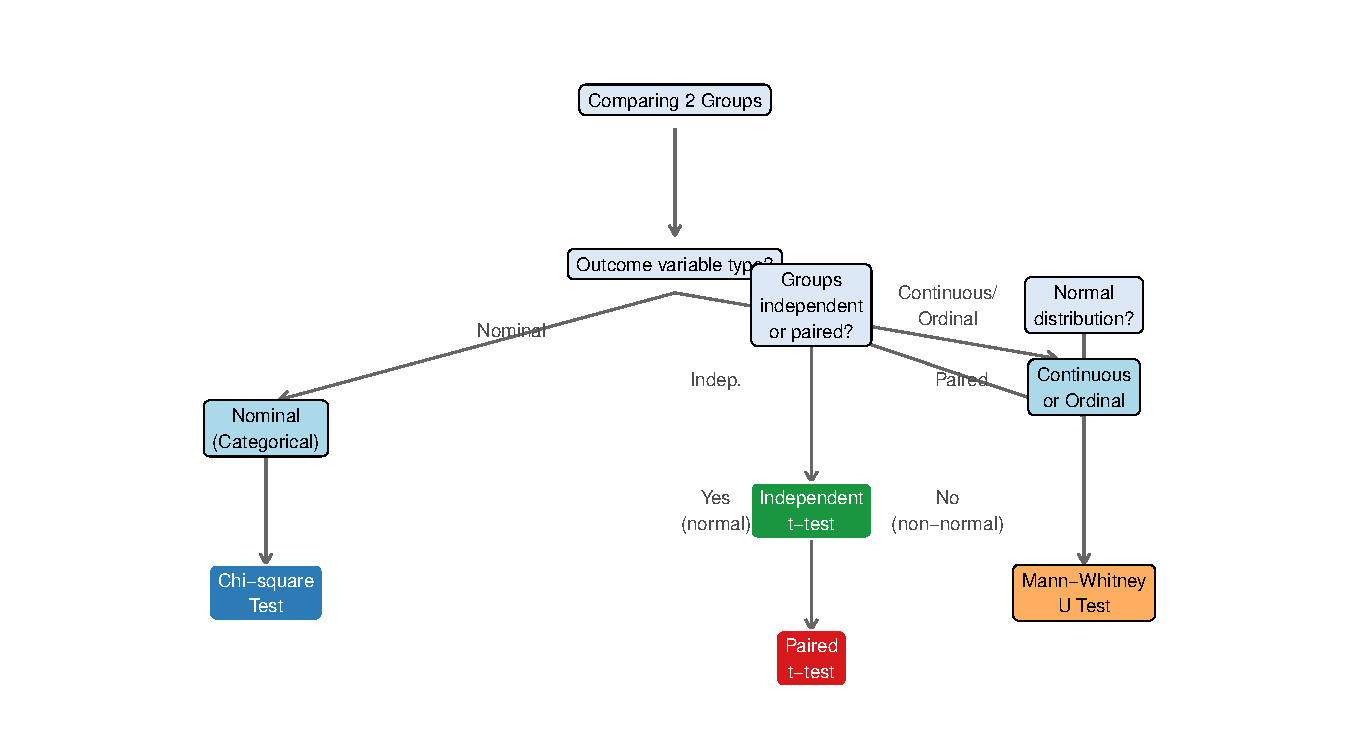
\includegraphics[keepaspectratio]{chapter05_statistical_testing_files/figure-pdf/fig-test-flowchart-1.pdf}}

}

\caption{\label{fig-test-flowchart}Decision flowchart for selecting the
correct test (two-group comparisons)}

\end{figure}%

\begin{center}\rule{0.5\linewidth}{0.5pt}\end{center}

\bookmarksetup{startatroot}

\chapter{Key Takeaways}\label{key-takeaways-4}

\begin{tcolorbox}[enhanced jigsaw, arc=.35mm, bottomrule=.15mm, bottomtitle=1mm, breakable, colback=white, colbacktitle=quarto-callout-note-color!10!white, colframe=quarto-callout-note-color-frame, coltitle=black, left=2mm, leftrule=.75mm, opacityback=0, opacitybacktitle=0.6, rightrule=.15mm, title={📝 Chapter 5 Summary}, titlerule=0mm, toprule=.15mm, toptitle=1mm]

\begin{enumerate}
\def\labelenumi{\arabic{enumi}.}
\item
  Hypothesis testing uses sample data to decide between two competing
  claims: the \textbf{null hypothesis (\(H_0\))} and the
  \textbf{alternative hypothesis (\(H_1\))}.
\item
  The \textbf{p-value} is the probability of the observed data (or more
  extreme) if \(H_0\) is true. A p-value \(\leq \alpha\) (usually 0.05)
  leads us to \textbf{reject \(H_0\)}.
\item
  \textbf{Type I error (α):} rejecting a true \(H_0\) (false positive).
  \textbf{Type II error (β):} failing to reject a false \(H_0\) (false
  negative).
\item
  \textbf{Chi-square test:} for association between two categorical
  (nominal) variables in independent groups.
\item
  \textbf{Mann-Whitney U test:} for comparing two independent groups
  when the outcome is ordinal or the normality assumption is not met.
\item
  \textbf{Independent samples t-test:} for comparing means of two
  independent groups with continuous, approximately normal data.
\item
  \textbf{Paired samples t-test:} for comparing means of two related
  measurements (before/after, or matched pairs) with continuous data.
\item
  Always choose the test based on \textbf{data type} and \textbf{study
  design} --- using the wrong test leads to invalid conclusions.
\end{enumerate}

\end{tcolorbox}

\begin{center}\rule{0.5\linewidth}{0.5pt}\end{center}

\bookmarksetup{startatroot}

\chapter{Examples}\label{examples-4}

\section{Example 1: Chi-Square Test}\label{example-1-chi-square-test}

A study investigates whether \textbf{smoking status} is associated with
\textbf{hypertension} in a sample of 200 adults.

{\def\LTcaptype{none} % do not increment counter
\begin{longtable}[]{@{}lccc@{}}
\toprule\noalign{}
& Hypertension & No Hypertension & Total \\
\midrule\noalign{}
\endhead
\bottomrule\noalign{}
\endlastfoot
Smoker & 45 & 55 & 100 \\
Non-smoker & 25 & 75 & 100 \\
\textbf{Total} & \textbf{70} & \textbf{130} & \textbf{200} \\
\end{longtable}
}

Test at \(\alpha = 0.05\) whether smoking is associated with
hypertension.

\begin{tcolorbox}[enhanced jigsaw, arc=.35mm, bottomrule=.15mm, bottomtitle=1mm, breakable, colback=white, colbacktitle=quarto-callout-tip-color!10!white, colframe=quarto-callout-tip-color-frame, coltitle=black, left=2mm, leftrule=.75mm, opacityback=0, opacitybacktitle=0.6, rightrule=.15mm, title={✅ Solution}, titlerule=0mm, toprule=.15mm, toptitle=1mm]

\textbf{Step 1 --- Hypotheses:}

\(H_0\): Smoking status and hypertension are independent (no
association).

\(H_1\): Smoking status and hypertension are associated.

\textbf{Step 2 ---} \(\alpha = 0.05\)

\textbf{Step 3 --- Expected frequencies:}

\[E = \frac{\text{Row total} \times \text{Column total}}{n}\]

\begin{Shaded}
\begin{Highlighting}[]
\NormalTok{obs }\OtherTok{\textless{}{-}} \FunctionTok{matrix}\NormalTok{(}\FunctionTok{c}\NormalTok{(}\DecValTok{45}\NormalTok{, }\DecValTok{55}\NormalTok{, }\DecValTok{25}\NormalTok{, }\DecValTok{75}\NormalTok{), }\AttributeTok{nrow=}\DecValTok{2}\NormalTok{, }\AttributeTok{byrow=}\ConstantTok{TRUE}\NormalTok{)}
\NormalTok{row\_totals }\OtherTok{\textless{}{-}} \FunctionTok{rowSums}\NormalTok{(obs)}
\NormalTok{col\_totals }\OtherTok{\textless{}{-}} \FunctionTok{colSums}\NormalTok{(obs)}
\NormalTok{n }\OtherTok{\textless{}{-}} \FunctionTok{sum}\NormalTok{(obs)}

\NormalTok{exp\_freq }\OtherTok{\textless{}{-}} \FunctionTok{outer}\NormalTok{(row\_totals, col\_totals) }\SpecialCharTok{/}\NormalTok{ n}

\NormalTok{result\_tab }\OtherTok{\textless{}{-}} \FunctionTok{data.frame}\NormalTok{(}
  \AttributeTok{Group =} \FunctionTok{c}\NormalTok{(}\StringTok{"Smoker"}\NormalTok{, }\StringTok{"Non{-}smoker"}\NormalTok{),}
  \AttributeTok{O\_hyp  =}\NormalTok{ obs[,}\DecValTok{1}\NormalTok{],}
  \AttributeTok{E\_hyp  =}\NormalTok{ exp\_freq[,}\DecValTok{1}\NormalTok{],}
  \AttributeTok{O\_no   =}\NormalTok{ obs[,}\DecValTok{2}\NormalTok{],}
  \AttributeTok{E\_no   =}\NormalTok{ exp\_freq[,}\DecValTok{2}\NormalTok{]}
\NormalTok{)}

\FunctionTok{kable}\NormalTok{(result\_tab,}
      \AttributeTok{col.names =} \FunctionTok{c}\NormalTok{(}\StringTok{"Group"}\NormalTok{,}\StringTok{"O (Hyp.)"}\NormalTok{,}\StringTok{"E (Hyp.)"}\NormalTok{,}\StringTok{"O (No Hyp.)"}\NormalTok{,}\StringTok{"E (No Hyp.)"}\NormalTok{),}
      \AttributeTok{align =} \FunctionTok{rep}\NormalTok{(}\StringTok{"c"}\NormalTok{,}\DecValTok{5}\NormalTok{), }\AttributeTok{digits =} \DecValTok{2}\NormalTok{) }\SpecialCharTok{|\textgreater{}}
  \FunctionTok{kable\_styling}\NormalTok{(}\AttributeTok{bootstrap\_options =} \FunctionTok{c}\NormalTok{(}\StringTok{"striped"}\NormalTok{,}\StringTok{"hover"}\NormalTok{,}\StringTok{"bordered"}\NormalTok{),}
                \AttributeTok{full\_width =} \ConstantTok{FALSE}\NormalTok{, }\AttributeTok{font\_size =} \DecValTok{13}\NormalTok{) }\SpecialCharTok{|\textgreater{}}
  \FunctionTok{column\_spec}\NormalTok{(}\DecValTok{1}\NormalTok{, }\AttributeTok{bold =} \ConstantTok{TRUE}\NormalTok{)}
\end{Highlighting}
\end{Shaded}

\begingroup\fontsize{13}{15}\selectfont

\begin{longtable}[t]{>{}ccccc}

\caption{\label{tbl-expected}Observed (O) and Expected (E) Frequencies}

\tabularnewline

\toprule
Group & O (Hyp.) & E (Hyp.) & O (No Hyp.) & E (No Hyp.)\\
\midrule
\textbf{Smoker} & 45 & 35 & 55 & 65\\
\textbf{Non-smoker} & 25 & 35 & 75 & 65\\
\bottomrule

\end{longtable}

\endgroup{}

All expected frequencies \(\geq 5\) ✓

\textbf{Step 4 --- Test statistic:}

\[\chi^2 = \frac{(45-35)^2}{35} + \frac{(55-65)^2}{65} +
           \frac{(25-35)^2}{35} + \frac{(75-65)^2}{65}\]

\[= \frac{100}{35} + \frac{100}{65} + \frac{100}{35} + \frac{100}{65}
= 2.857 + 1.538 + 2.857 + 1.538 = \mathbf{8.791}\]

\(df = (2-1)(2-1) = 1\)

\textbf{Step 5 --- Decision:}

From the chi-square table: \(\chi^2_{\text{critical}} = 3.841\) at
\(df=1\), \(\alpha=0.05\).

Since \(8.791 > 3.841\), we \textbf{reject \(H_0\)}.

The p-value \(= 0.003 < 0.05\).

\textbf{Conclusion:} There is a statistically significant association
between smoking status and hypertension (\(\chi^2 = 8.79\), \(df = 1\),
\(p = 0.003\)). Smokers have a higher prevalence of hypertension than
non-smokers.

\end{tcolorbox}

\begin{center}\rule{0.5\linewidth}{0.5pt}\end{center}

\section{Example 2: Independent Samples
t-Test}\label{example-2-independent-samples-t-test}

A clinical trial compares the mean reduction in systolic blood pressure
(mmHg) between patients receiving a \textbf{new drug} vs.~a
\textbf{placebo} after 8 weeks.

{\def\LTcaptype{none} % do not increment counter
\begin{longtable}[]{@{}lccc@{}}
\toprule\noalign{}
Group & n & Mean reduction & SD \\
\midrule\noalign{}
\endhead
\bottomrule\noalign{}
\endlastfoot
New drug & 40 & 12.4 & 6.8 \\
Placebo & 40 & 7.1 & 7.2 \\
\end{longtable}
}

Test at \(\alpha = 0.05\) whether the new drug produces a greater mean
reduction in SBP than placebo.

\begin{tcolorbox}[enhanced jigsaw, arc=.35mm, bottomrule=.15mm, bottomtitle=1mm, breakable, colback=white, colbacktitle=quarto-callout-tip-color!10!white, colframe=quarto-callout-tip-color-frame, coltitle=black, left=2mm, leftrule=.75mm, opacityback=0, opacitybacktitle=0.6, rightrule=.15mm, title={✅ Solution}, titlerule=0mm, toprule=.15mm, toptitle=1mm]

\textbf{Step 1 --- Hypotheses:}

\(H_0: \mu_1 = \mu_2\) (no difference in mean reduction)

\(H_1: \mu_1 \neq \mu_2\) (two-tailed; difference exists)

\textbf{Step 2 ---} \(\alpha = 0.05\)

\textbf{Step 3 --- Pooled standard error} (assuming equal variances):

\[s_p = \sqrt{\frac{(40-1)(6.8)^2 + (40-1)(7.2)^2}{40+40-2}}
= \sqrt{\frac{39(46.24) + 39(51.84)}{78}}
= \sqrt{\frac{1803.36 + 2021.76}{78}}
= \sqrt{49.041} = 7.003\]

\[SE = 7.003 \times \sqrt{\frac{1}{40}+\frac{1}{40}}
= 7.003 \times \sqrt{0.05}
= 7.003 \times 0.2236 = 1.566\]

\textbf{Step 4 --- Test statistic:}

\[t = \frac{12.4 - 7.1}{1.566} = \frac{5.3}{1.566} = \mathbf{3.384}\]

\(df = 40 + 40 - 2 = 78\)

\textbf{Step 5 --- Decision:}

\(t_{\text{critical}} = 1.991\) at \(df = 78\), \(\alpha = 0.05\)
(two-tailed).

Since \(3.384 > 1.991\), we \textbf{reject \(H_0\)}.

The p-value \(= 0.001 < 0.05\).

\textbf{Conclusion:} The new drug produces a significantly greater
reduction in systolic blood pressure compared to placebo (\(t = 3.38\),
\(df = 78\), \(p = 0.001\)). The mean difference is 5.3 mmHg (95\% CI:
2.2 to 8.4 mmHg).

\end{tcolorbox}

\begin{center}\rule{0.5\linewidth}{0.5pt}\end{center}

\section{Example 3: Paired Samples
t-Test}\label{example-3-paired-samples-t-test}

A study measures the \textbf{diastolic blood pressure (DBP)} of 10
patients \textbf{before} and \textbf{after} 4 weeks of a lifestyle
intervention.

\begin{Shaded}
\begin{Highlighting}[]
\FunctionTok{set.seed}\NormalTok{(}\DecValTok{7}\NormalTok{)}
\NormalTok{before }\OtherTok{\textless{}{-}} \FunctionTok{c}\NormalTok{(}\DecValTok{92}\NormalTok{, }\DecValTok{88}\NormalTok{, }\DecValTok{95}\NormalTok{, }\DecValTok{100}\NormalTok{, }\DecValTok{85}\NormalTok{, }\DecValTok{97}\NormalTok{, }\DecValTok{90}\NormalTok{, }\DecValTok{94}\NormalTok{, }\DecValTok{88}\NormalTok{, }\DecValTok{96}\NormalTok{)}
\NormalTok{after  }\OtherTok{\textless{}{-}} \FunctionTok{c}\NormalTok{(}\DecValTok{85}\NormalTok{, }\DecValTok{82}\NormalTok{, }\DecValTok{89}\NormalTok{, }\DecValTok{91}\NormalTok{,  }\DecValTok{80}\NormalTok{, }\DecValTok{88}\NormalTok{, }\DecValTok{84}\NormalTok{, }\DecValTok{87}\NormalTok{, }\DecValTok{83}\NormalTok{, }\DecValTok{88}\NormalTok{)}
\NormalTok{d      }\OtherTok{\textless{}{-}}\NormalTok{ before }\SpecialCharTok{{-}}\NormalTok{ after}

\NormalTok{pair\_tab }\OtherTok{\textless{}{-}} \FunctionTok{data.frame}\NormalTok{(}
  \AttributeTok{Patient =} \FunctionTok{paste0}\NormalTok{(}\StringTok{"Patient "}\NormalTok{, }\DecValTok{1}\SpecialCharTok{:}\DecValTok{10}\NormalTok{),}
  \AttributeTok{Before  =}\NormalTok{ before,}
  \AttributeTok{After   =}\NormalTok{ after,}
  \AttributeTok{d       =}\NormalTok{ d}
\NormalTok{)}

\FunctionTok{kable}\NormalTok{(pair\_tab,}
      \AttributeTok{col.names =} \FunctionTok{c}\NormalTok{(}\StringTok{"Patient"}\NormalTok{, }\StringTok{"DBP Before (mmHg)"}\NormalTok{,}
                    \StringTok{"DBP After (mmHg)"}\NormalTok{, }\StringTok{"Difference d = Before − After"}\NormalTok{),}
      \AttributeTok{align =} \FunctionTok{c}\NormalTok{(}\StringTok{"l"}\NormalTok{,}\StringTok{"c"}\NormalTok{,}\StringTok{"c"}\NormalTok{,}\StringTok{"c"}\NormalTok{)) }\SpecialCharTok{|\textgreater{}}
  \FunctionTok{kable\_styling}\NormalTok{(}\AttributeTok{bootstrap\_options =} \FunctionTok{c}\NormalTok{(}\StringTok{"striped"}\NormalTok{,}\StringTok{"hover"}\NormalTok{,}\StringTok{"bordered"}\NormalTok{),}
                \AttributeTok{full\_width =} \ConstantTok{FALSE}\NormalTok{, }\AttributeTok{font\_size =} \DecValTok{13}\NormalTok{) }\SpecialCharTok{|\textgreater{}}
  \FunctionTok{column\_spec}\NormalTok{(}\DecValTok{4}\NormalTok{, }\AttributeTok{bold =} \ConstantTok{TRUE}\NormalTok{, }\AttributeTok{color =} \StringTok{"\#2c7bb6"}\NormalTok{) }\SpecialCharTok{|\textgreater{}}
  \FunctionTok{row\_spec}\NormalTok{(}\DecValTok{0}\NormalTok{, }\AttributeTok{bold =} \ConstantTok{TRUE}\NormalTok{, }\AttributeTok{color =} \StringTok{"white"}\NormalTok{, }\AttributeTok{background =} \StringTok{"\#2c7bb6"}\NormalTok{)}
\end{Highlighting}
\end{Shaded}

\begingroup\fontsize{13}{15}\selectfont

\begin{longtable}[t]{lcc>{}c}

\caption{\label{tbl-paired}DBP Before and After Lifestyle Intervention
(n = 10 patients)}

\tabularnewline

\toprule
\cellcolor[HTML]{2c7bb6}{\textcolor{white}{\textbf{Patient}}} & \cellcolor[HTML]{2c7bb6}{\textcolor{white}{\textbf{DBP Before (mmHg)}}} & \cellcolor[HTML]{2c7bb6}{\textcolor{white}{\textbf{DBP After (mmHg)}}} & \cellcolor[HTML]{2c7bb6}{\textcolor{white}{\textbf{Difference d = Before − After}}}\\
\midrule
Patient 1 & 92 & 85 & \textcolor[HTML]{2c7bb6}{\textbf{7}}\\
Patient 2 & 88 & 82 & \textcolor[HTML]{2c7bb6}{\textbf{6}}\\
Patient 3 & 95 & 89 & \textcolor[HTML]{2c7bb6}{\textbf{6}}\\
Patient 4 & 100 & 91 & \textcolor[HTML]{2c7bb6}{\textbf{9}}\\
Patient 5 & 85 & 80 & \textcolor[HTML]{2c7bb6}{\textbf{5}}\\
\addlinespace
Patient 6 & 97 & 88 & \textcolor[HTML]{2c7bb6}{\textbf{9}}\\
Patient 7 & 90 & 84 & \textcolor[HTML]{2c7bb6}{\textbf{6}}\\
Patient 8 & 94 & 87 & \textcolor[HTML]{2c7bb6}{\textbf{7}}\\
Patient 9 & 88 & 83 & \textcolor[HTML]{2c7bb6}{\textbf{5}}\\
Patient 10 & 96 & 88 & \textcolor[HTML]{2c7bb6}{\textbf{8}}\\
\bottomrule

\end{longtable}

\endgroup{}

Test at \(\alpha = 0.05\) whether the intervention significantly reduces
DBP.

\begin{tcolorbox}[enhanced jigsaw, arc=.35mm, bottomrule=.15mm, bottomtitle=1mm, breakable, colback=white, colbacktitle=quarto-callout-tip-color!10!white, colframe=quarto-callout-tip-color-frame, coltitle=black, left=2mm, leftrule=.75mm, opacityback=0, opacitybacktitle=0.6, rightrule=.15mm, title={✅ Solution}, titlerule=0mm, toprule=.15mm, toptitle=1mm]

\textbf{Step 1 --- Hypotheses:}

\(H_0: \mu_d = 0\) (no mean change in DBP)

\(H_1: \mu_d \neq 0\) (mean DBP has changed)

\textbf{Step 2 ---} \(\alpha = 0.05\)

\textbf{Step 3 --- Compute \(\bar{d}\) and \(s_d\):}

\[\bar{d} = \frac{68}{10} = 6.8 \text{ mmHg}\]

\[s_d = \sqrt{\frac{\sum(d_i - \bar{d})^2}{n-1}} = 1.476\]

\textbf{Step 4 --- Test statistic:}

\[t = \frac{\bar{d}}{s_d/\sqrt{n}} = \frac{6.8}{1.476/\sqrt{10}}
= \frac{6.8}{0.467} = 14.571\]

\(df = n - 1 = 9\)

\textbf{Step 5 --- Decision:}

\(t_{\text{critical}} = 2.262\) at \(df = 9\), \(\alpha = 0.05\)
(two-tailed).

Since \(14.571 > 2.262\), we \textbf{reject \(H_0\)}.

\textbf{Conclusion:} The lifestyle intervention produced a statistically
significant reduction in diastolic blood pressure (\(t = 14.57\),
\(df = 9\), \(p < 0.05\)). The mean reduction was \textbf{6.8 mmHg}.

\end{tcolorbox}

\begin{center}\rule{0.5\linewidth}{0.5pt}\end{center}

\bookmarksetup{startatroot}

\chapter{Exercises}\label{exercises-4}

\begin{tcolorbox}[enhanced jigsaw, arc=.35mm, bottomrule=.15mm, bottomtitle=1mm, breakable, colback=white, colbacktitle=quarto-callout-caution-color!10!white, colframe=quarto-callout-caution-color-frame, coltitle=black, left=2mm, leftrule=.75mm, opacityback=0, opacitybacktitle=0.6, rightrule=.15mm, title={✏️ Exercise 1 --- Chi-Square Test}, titlerule=0mm, toprule=.15mm, toptitle=1mm]

A researcher investigates whether \textbf{physical activity level} is
associated with \textbf{diabetes status} in 300 adults:

{\def\LTcaptype{none} % do not increment counter
\begin{longtable}[]{@{}lccc@{}}
\toprule\noalign{}
& Diabetes & No Diabetes & Total \\
\midrule\noalign{}
\endhead
\bottomrule\noalign{}
\endlastfoot
Active & 18 & 132 & 150 \\
Inactive & 42 & 108 & 150 \\
\textbf{Total} & \textbf{60} & \textbf{240} & \textbf{300} \\
\end{longtable}
}

\textbf{(a)} State \(H_0\) and \(H_1\).

\textbf{(b)} Calculate all expected frequencies and verify the
chi-square condition is met.

\textbf{(c)} Calculate the chi-square test statistic.

\textbf{(d)} At \(\alpha = 0.05\), what is your conclusion?

\textbf{(e)} In plain language, what does your result mean?

\end{tcolorbox}

\begin{tcolorbox}[enhanced jigsaw, arc=.35mm, bottomrule=.15mm, bottomtitle=1mm, breakable, colback=white, colbacktitle=quarto-callout-caution-color!10!white, colframe=quarto-callout-caution-color-frame, coltitle=black, left=2mm, leftrule=.75mm, opacityback=0, opacitybacktitle=0.6, rightrule=.15mm, title={✏️ Exercise 2 --- Independent Samples t-Test}, titlerule=0mm, toprule=.15mm, toptitle=1mm]

A study compares the \textbf{mean hemoglobin levels (g/dL)} between male
and female patients:

{\def\LTcaptype{none} % do not increment counter
\begin{longtable}[]{@{}lccc@{}}
\toprule\noalign{}
Group & n & \(\bar{x}\) & s \\
\midrule\noalign{}
\endhead
\bottomrule\noalign{}
\endlastfoot
Male & 35 & 14.8 & 1.6 \\
Female & 35 & 12.9 & 1.4 \\
\end{longtable}
}

\textbf{(a)} State \(H_0\) and \(H_1\) (two-tailed).

\textbf{(b)} Calculate the pooled standard error.

\textbf{(c)} Calculate the t test statistic.

\textbf{(d)} At \(\alpha = 0.05\) with appropriate df, state your
conclusion.

\end{tcolorbox}

\begin{tcolorbox}[enhanced jigsaw, arc=.35mm, bottomrule=.15mm, bottomtitle=1mm, breakable, colback=white, colbacktitle=quarto-callout-caution-color!10!white, colframe=quarto-callout-caution-color-frame, coltitle=black, left=2mm, leftrule=.75mm, opacityback=0, opacitybacktitle=0.6, rightrule=.15mm, title={✏️ Exercise 3 --- Paired Samples t-Test}, titlerule=0mm, toprule=.15mm, toptitle=1mm]

A pain management study measures the \textbf{pain score (0--10)} of 8
patients \textbf{before} and \textbf{one hour after} receiving an
analgesic:

{\def\LTcaptype{none} % do not increment counter
\begin{longtable}[]{@{}lcccccccc@{}}
\toprule\noalign{}
Patient & 1 & 2 & 3 & 4 & 5 & 6 & 7 & 8 \\
\midrule\noalign{}
\endhead
\bottomrule\noalign{}
\endlastfoot
Before & 7 & 8 & 6 & 9 & 7 & 8 & 5 & 9 \\
After & 4 & 5 & 4 & 6 & 3 & 5 & 3 & 6 \\
\end{longtable}
}

\textbf{(a)} Calculate the difference \(d_i\) for each patient.

\textbf{(b)} Calculate \(\bar{d}\) and \(s_d\).

\textbf{(c)} Calculate the paired t statistic.

\textbf{(d)} At \(\alpha = 0.05\), is the analgesic effective in
reducing pain? State your conclusion clearly.

\end{tcolorbox}

\begin{tcolorbox}[enhanced jigsaw, arc=.35mm, bottomrule=.15mm, bottomtitle=1mm, breakable, colback=white, colbacktitle=quarto-callout-caution-color!10!white, colframe=quarto-callout-caution-color-frame, coltitle=black, left=2mm, leftrule=.75mm, opacityback=0, opacitybacktitle=0.6, rightrule=.15mm, title={✏️ Exercise 4 --- Choosing the Right Test}, titlerule=0mm, toprule=.15mm, toptitle=1mm]

For each scenario below, state which statistical test is most
appropriate and briefly explain why:

\textbf{(a)} Comparing the proportion of post-operative complications
between patients who received standard care vs.~enhanced recovery
protocol.

\textbf{(b)} Comparing patient satisfaction scores (rated: Poor / Fair /
Good / Excellent) between two hospital wards.

\textbf{(c)} Measuring the effect of a new diet on body weight by
recording each participant's weight before and after a 12-week program.

\textbf{(d)} Comparing the mean length of hospital stay (days) between
two age groups (under 60 vs.~60 and over), where length-of-stay data is
strongly right-skewed.

\end{tcolorbox}

\begin{center}\rule{0.5\linewidth}{0.5pt}\end{center}

\emph{End of Chapter 5}

\begin{center}\rule{0.5\linewidth}{0.5pt}\end{center}

\begin{tcolorbox}[enhanced jigsaw, arc=.35mm, bottomrule=.15mm, bottomtitle=1mm, breakable, colback=white, colbacktitle=quarto-callout-note-color!10!white, colframe=quarto-callout-note-color-frame, coltitle=black, left=2mm, leftrule=.75mm, opacityback=0, opacitybacktitle=0.6, rightrule=.15mm, title={📚 Coming Up Next}, titlerule=0mm, toprule=.15mm, toptitle=1mm]

\textbf{Chapter 6: Introduction to Statistical Modeling} --- We take our
first steps beyond comparing two groups, exploring how one variable can
be used to explain or predict another through \textbf{linear
regression}.

\end{tcolorbox}

\bookmarksetup{startatroot}

\chapter{Introduction to Statistical
Modeling}\label{introduction-to-statistical-modeling}

\begin{center}\rule{0.5\linewidth}{0.5pt}\end{center}

\bookmarksetup{startatroot}

\chapter*{Introduction}\label{introduction-5}
\addcontentsline{toc}{chapter}{Introduction}

\markboth{Introduction}{Introduction}

\begin{tcolorbox}[enhanced jigsaw, arc=.35mm, bottomrule=.15mm, bottomtitle=1mm, breakable, colback=white, colbacktitle=quarto-callout-note-color!10!white, colframe=quarto-callout-note-color-frame, coltitle=black, left=2mm, leftrule=.75mm, opacityback=0, opacitybacktitle=0.6, rightrule=.15mm, title={💡 Why Does This Matter?}, titlerule=0mm, toprule=.15mm, toptitle=1mm]

So far we have described data, estimated population parameters, and
tested whether two groups differ. But many real-world health questions
go beyond simple comparisons:

\begin{itemize}
\tightlist
\item
  Does body weight \emph{predict} blood pressure?
\item
  As age \emph{increases}, how does cholesterol \emph{change}?
\item
  Can we use a patient's BMI to \emph{estimate} their fasting glucose
  level?
\end{itemize}

These questions require us to model the \textbf{relationship between two
variables}. \textbf{Statistical modeling} is the process of building a
mathematical equation that describes how one variable is related to
another --- and using that equation to understand, explain, and predict
outcomes.

In this chapter we focus on the simplest and most widely used model:
\textbf{simple linear regression}.

\end{tcolorbox}

\begin{center}\rule{0.5\linewidth}{0.5pt}\end{center}

\bookmarksetup{startatroot}

\chapter{What Is a Statistical
Model?}\label{what-is-a-statistical-model}

A \textbf{statistical model} is a mathematical equation that describes
the relationship between:

\begin{itemize}
\tightlist
\item
  An \textbf{outcome variable} (also called the \emph{dependent
  variable}, \emph{response variable}, or \(Y\)) --- the variable we
  want to explain or predict.
\item
  One or more \textbf{predictor variables} (also called
  \emph{independent variables}, \emph{explanatory variables}, or \(X\))
  --- the variables we use to explain or predict \(Y\).
\end{itemize}

In this chapter we study \textbf{simple linear regression} --- one
outcome \(Y\) and one predictor \(X\), with a straight-line
relationship.

\begin{center}\rule{0.5\linewidth}{0.5pt}\end{center}

\bookmarksetup{startatroot}

\chapter{Correlation: Measuring the
Relationship}\label{correlation-measuring-the-relationship}

Before building a model, we first ask: \emph{Is there a relationship
between \(X\) and \(Y\), and how strong is it?}

\section{The Scatter Plot}\label{the-scatter-plot}

A \textbf{scatter plot} displays pairs of values \((x_i, y_i)\) as
points on a graph. The pattern of points reveals the \textbf{direction}
and \textbf{strength} of the relationship.

\begin{Shaded}
\begin{Highlighting}[]
\FunctionTok{set.seed}\NormalTok{(}\DecValTok{42}\NormalTok{)}
\NormalTok{n }\OtherTok{\textless{}{-}} \DecValTok{80}

\NormalTok{d1 }\OtherTok{\textless{}{-}} \FunctionTok{data.frame}\NormalTok{(}\AttributeTok{x =} \FunctionTok{rnorm}\NormalTok{(n), }\AttributeTok{y =} \FloatTok{0.8}\SpecialCharTok{*}\FunctionTok{rnorm}\NormalTok{(n, }\AttributeTok{mean=}\DecValTok{0}\NormalTok{) }\SpecialCharTok{+} \FunctionTok{rnorm}\NormalTok{(n,}\AttributeTok{sd=}\FloatTok{0.5}\NormalTok{),}
                 \AttributeTok{type =} \StringTok{"Strong positive"}\NormalTok{)}
\NormalTok{d1}\SpecialCharTok{$}\NormalTok{y }\OtherTok{\textless{}{-}}\NormalTok{ d1}\SpecialCharTok{$}\NormalTok{x }\SpecialCharTok{*} \FloatTok{0.9} \SpecialCharTok{+} \FunctionTok{rnorm}\NormalTok{(n, }\AttributeTok{sd=}\FloatTok{0.3}\NormalTok{)}

\NormalTok{d2 }\OtherTok{\textless{}{-}} \FunctionTok{data.frame}\NormalTok{(}\AttributeTok{x =} \FunctionTok{rnorm}\NormalTok{(n), }\AttributeTok{y =} \SpecialCharTok{{-}}\FloatTok{0.9}\SpecialCharTok{*}\FunctionTok{rnorm}\NormalTok{(n) }\SpecialCharTok{+} \FunctionTok{rnorm}\NormalTok{(n,}\AttributeTok{sd=}\FloatTok{0.3}\NormalTok{),}
                 \AttributeTok{type =} \StringTok{"Strong negative"}\NormalTok{)}
\NormalTok{d2}\SpecialCharTok{$}\NormalTok{y }\OtherTok{\textless{}{-}} \SpecialCharTok{{-}}\NormalTok{d2}\SpecialCharTok{$}\NormalTok{x }\SpecialCharTok{*} \FloatTok{0.9} \SpecialCharTok{+} \FunctionTok{rnorm}\NormalTok{(n, }\AttributeTok{sd=}\FloatTok{0.3}\NormalTok{)}

\NormalTok{d3 }\OtherTok{\textless{}{-}} \FunctionTok{data.frame}\NormalTok{(}\AttributeTok{x =} \FunctionTok{rnorm}\NormalTok{(n), }\AttributeTok{y =} \FloatTok{0.4}\SpecialCharTok{*}\FunctionTok{rnorm}\NormalTok{(n) }\SpecialCharTok{+} \FunctionTok{rnorm}\NormalTok{(n,}\AttributeTok{sd=}\FloatTok{0.9}\NormalTok{),}
                 \AttributeTok{type =} \StringTok{"Weak positive"}\NormalTok{)}
\NormalTok{d3}\SpecialCharTok{$}\NormalTok{y }\OtherTok{\textless{}{-}}\NormalTok{ d3}\SpecialCharTok{$}\NormalTok{x }\SpecialCharTok{*} \FloatTok{0.3} \SpecialCharTok{+} \FunctionTok{rnorm}\NormalTok{(n, }\AttributeTok{sd=}\FloatTok{0.9}\NormalTok{)}

\NormalTok{d4 }\OtherTok{\textless{}{-}} \FunctionTok{data.frame}\NormalTok{(}\AttributeTok{x =} \FunctionTok{rnorm}\NormalTok{(n), }\AttributeTok{y =} \FunctionTok{rnorm}\NormalTok{(n),}
                 \AttributeTok{type =} \StringTok{"No relationship"}\NormalTok{)}

\NormalTok{all\_d }\OtherTok{\textless{}{-}} \FunctionTok{rbind}\NormalTok{(d1, d2, d3, d4)}
\NormalTok{all\_d}\SpecialCharTok{$}\NormalTok{type }\OtherTok{\textless{}{-}} \FunctionTok{factor}\NormalTok{(all\_d}\SpecialCharTok{$}\NormalTok{type,}
                     \AttributeTok{levels =} \FunctionTok{c}\NormalTok{(}\StringTok{"Strong positive"}\NormalTok{,}\StringTok{"Strong negative"}\NormalTok{,}
                                \StringTok{"Weak positive"}\NormalTok{,}\StringTok{"No relationship"}\NormalTok{))}

\FunctionTok{ggplot}\NormalTok{(all\_d, }\FunctionTok{aes}\NormalTok{(}\AttributeTok{x =}\NormalTok{ x, }\AttributeTok{y =}\NormalTok{ y)) }\SpecialCharTok{+}
  \FunctionTok{geom\_point}\NormalTok{(}\AttributeTok{alpha =} \FloatTok{0.5}\NormalTok{, }\AttributeTok{color =} \StringTok{"\#2c7bb6"}\NormalTok{, }\AttributeTok{size =} \FloatTok{1.5}\NormalTok{) }\SpecialCharTok{+}
  \FunctionTok{geom\_smooth}\NormalTok{(}\AttributeTok{method =} \StringTok{"lm"}\NormalTok{, }\AttributeTok{se =} \ConstantTok{FALSE}\NormalTok{, }\AttributeTok{color =} \StringTok{"\#d7191c"}\NormalTok{,}
              \AttributeTok{linewidth =} \DecValTok{1}\NormalTok{, }\AttributeTok{formula =}\NormalTok{ y }\SpecialCharTok{\textasciitilde{}}\NormalTok{ x) }\SpecialCharTok{+}
  \FunctionTok{facet\_wrap}\NormalTok{(}\SpecialCharTok{\textasciitilde{}}\NormalTok{ type, }\AttributeTok{nrow =} \DecValTok{1}\NormalTok{, }\AttributeTok{scales =} \StringTok{"free"}\NormalTok{) }\SpecialCharTok{+}
  \FunctionTok{theme\_minimal}\NormalTok{(}\AttributeTok{base\_size =} \DecValTok{12}\NormalTok{) }\SpecialCharTok{+}
  \FunctionTok{theme}\NormalTok{(}\AttributeTok{axis.text =} \FunctionTok{element\_blank}\NormalTok{(),}
        \AttributeTok{axis.ticks =} \FunctionTok{element\_blank}\NormalTok{(),}
        \AttributeTok{axis.title =} \FunctionTok{element\_blank}\NormalTok{(),}
        \AttributeTok{panel.grid =} \FunctionTok{element\_blank}\NormalTok{(),}
        \AttributeTok{strip.text =} \FunctionTok{element\_text}\NormalTok{(}\AttributeTok{face =} \StringTok{"bold"}\NormalTok{, }\AttributeTok{size =} \DecValTok{11}\NormalTok{))}
\end{Highlighting}
\end{Shaded}

\begin{figure}[H]

\centering{

\pandocbounded{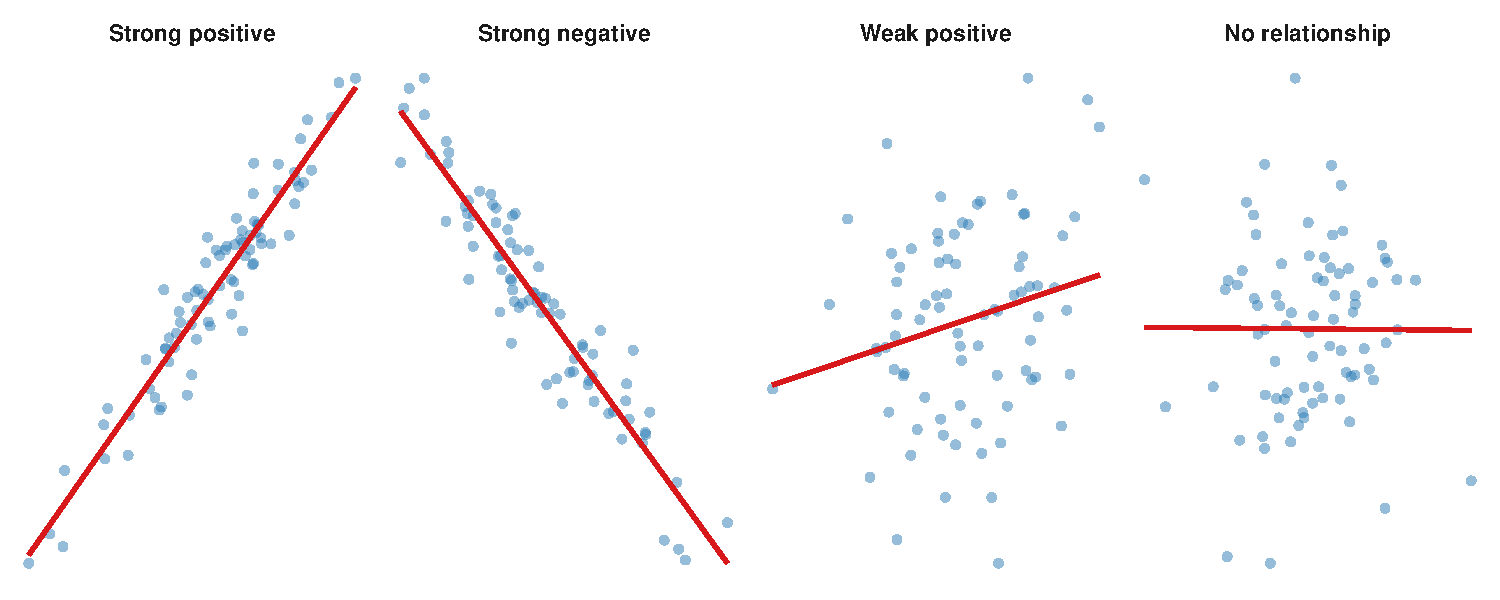
\includegraphics[keepaspectratio]{chapter06_statistical_modeling_files/figure-pdf/fig-scatter-types-1.pdf}}

}

\caption{\label{fig-scatter-types}Four possible relationships between
two variables}

\end{figure}%

\begin{center}\rule{0.5\linewidth}{0.5pt}\end{center}

\section{\texorpdfstring{Pearson's Correlation Coefficient
(\(r\))}{Pearson's Correlation Coefficient (r)}}\label{pearsons-correlation-coefficient-r}

The \textbf{Pearson correlation coefficient} \(r\) quantifies the
\textbf{strength} and \textbf{direction} of the \emph{linear}
relationship between two continuous variables.

\[r = \frac{\sum_{i=1}^{n}(x_i - \bar{x})(y_i - \bar{y})}
           {\sqrt{\sum_{i=1}^{n}(x_i-\bar{x})^2 \cdot \sum_{i=1}^{n}(y_i-\bar{y})^2}}\]

\subsection{\texorpdfstring{Properties of
\(r\)}{Properties of r}}\label{properties-of-r}

\begin{itemize}
\tightlist
\item
  \(r\) always lies between \textbf{−1 and +1}
\item
  \(r = +1\): perfect positive linear relationship
\item
  \(r = -1\): perfect negative linear relationship
\item
  \(r = 0\): no linear relationship
\end{itemize}

\subsection{\texorpdfstring{Interpreting the Magnitude of
\(r\)}{Interpreting the Magnitude of r}}\label{interpreting-the-magnitude-of-r}

\begin{Shaded}
\begin{Highlighting}[]
\NormalTok{r\_tab }\OtherTok{\textless{}{-}} \FunctionTok{data.frame}\NormalTok{(}
  \StringTok{\textasciigrave{}}\AttributeTok{|r| range}\StringTok{\textasciigrave{}} \OtherTok{=} \FunctionTok{c}\NormalTok{(}\StringTok{"0.00 – 0.19"}\NormalTok{, }\StringTok{"0.20 – 0.39"}\NormalTok{,}
                   \StringTok{"0.40 – 0.59"}\NormalTok{, }\StringTok{"0.60 – 0.79"}\NormalTok{, }\StringTok{"0.80 – 1.00"}\NormalTok{),}
  \AttributeTok{Strength =} \FunctionTok{c}\NormalTok{(}\StringTok{"Negligible"}\NormalTok{, }\StringTok{"Weak"}\NormalTok{, }\StringTok{"Moderate"}\NormalTok{, }\StringTok{"Strong"}\NormalTok{, }\StringTok{"Very strong"}\NormalTok{),}
  \AttributeTok{Direction =} \FunctionTok{c}\NormalTok{(}\StringTok{"—"}\NormalTok{, }\StringTok{"Positive or negative depending on sign"}\NormalTok{,}
                \StringTok{"Positive or negative depending on sign"}\NormalTok{,}
                \StringTok{"Positive or negative depending on sign"}\NormalTok{,}
                \StringTok{"Positive or negative depending on sign"}\NormalTok{)}
\NormalTok{)}

\FunctionTok{kable}\NormalTok{(r\_tab, }\AttributeTok{col.names =} \FunctionTok{c}\NormalTok{(}\StringTok{"|r| value"}\NormalTok{, }\StringTok{"Strength"}\NormalTok{, }\StringTok{"Note"}\NormalTok{),}
      \AttributeTok{align =} \FunctionTok{c}\NormalTok{(}\StringTok{"c"}\NormalTok{,}\StringTok{"l"}\NormalTok{,}\StringTok{"l"}\NormalTok{)) }\SpecialCharTok{|\textgreater{}}
  \FunctionTok{kable\_styling}\NormalTok{(}\AttributeTok{bootstrap\_options =} \FunctionTok{c}\NormalTok{(}\StringTok{"striped"}\NormalTok{,}\StringTok{"hover"}\NormalTok{,}\StringTok{"bordered"}\NormalTok{),}
                \AttributeTok{full\_width =} \ConstantTok{FALSE}\NormalTok{, }\AttributeTok{font\_size =} \DecValTok{13}\NormalTok{) }\SpecialCharTok{|\textgreater{}}
  \FunctionTok{column\_spec}\NormalTok{(}\DecValTok{1}\NormalTok{, }\AttributeTok{bold =} \ConstantTok{TRUE}\NormalTok{, }\AttributeTok{color =} \StringTok{"\#2c7bb6"}\NormalTok{)}
\end{Highlighting}
\end{Shaded}

\begingroup\fontsize{13}{15}\selectfont

\begin{longtable}[t]{>{}cll}

\caption{\label{tbl-r-interpret}General guidelines for interpreting the
correlation coefficient}

\tabularnewline

\toprule
\&\#124;r\&\#124; value & Strength & Note\\
\midrule
\textcolor[HTML]{2c7bb6}{\textbf{0.00 – 0.19}} & Negligible & —\\
\textcolor[HTML]{2c7bb6}{\textbf{0.20 – 0.39}} & Weak & Positive or negative depending on sign\\
\textcolor[HTML]{2c7bb6}{\textbf{0.40 – 0.59}} & Moderate & Positive or negative depending on sign\\
\textcolor[HTML]{2c7bb6}{\textbf{0.60 – 0.79}} & Strong & Positive or negative depending on sign\\
\textcolor[HTML]{2c7bb6}{\textbf{0.80 – 1.00}} & Very strong & Positive or negative depending on sign\\
\bottomrule

\end{longtable}

\endgroup{}

\begin{tcolorbox}[enhanced jigsaw, arc=.35mm, bottomrule=.15mm, bottomtitle=1mm, breakable, colback=white, colbacktitle=quarto-callout-warning-color!10!white, colframe=quarto-callout-warning-color-frame, coltitle=black, left=2mm, leftrule=.75mm, opacityback=0, opacitybacktitle=0.6, rightrule=.15mm, title={⚠️ Correlation Is Not Causation}, titlerule=0mm, toprule=.15mm, toptitle=1mm]

A high correlation between \(X\) and \(Y\) does \textbf{not} mean that
\(X\) \emph{causes} \(Y\). Both variables may be influenced by a third
variable, or the relationship may be coincidental. Always interpret
correlations in the context of biological or clinical plausibility.

\end{tcolorbox}

\begin{center}\rule{0.5\linewidth}{0.5pt}\end{center}

\bookmarksetup{startatroot}

\chapter{Simple Linear Regression}\label{simple-linear-regression}

\section{The Regression Equation}\label{the-regression-equation}

Simple linear regression models the relationship between \(X\) and \(Y\)
as a straight line:

\[\hat{Y} = b_0 + b_1 X\]

Where:

{\def\LTcaptype{none} % do not increment counter
\begin{longtable}[]{@{}
  >{\centering\arraybackslash}p{(\linewidth - 4\tabcolsep) * \real{0.4545}}
  >{\raggedright\arraybackslash}p{(\linewidth - 4\tabcolsep) * \real{0.2727}}
  >{\raggedright\arraybackslash}p{(\linewidth - 4\tabcolsep) * \real{0.2727}}@{}}
\toprule\noalign{}
\begin{minipage}[b]{\linewidth}\centering
Symbol
\end{minipage} & \begin{minipage}[b]{\linewidth}\raggedright
Name
\end{minipage} & \begin{minipage}[b]{\linewidth}\raggedright
Meaning
\end{minipage} \\
\midrule\noalign{}
\endhead
\bottomrule\noalign{}
\endlastfoot
\(\hat{Y}\) & Predicted value & The estimated value of \(Y\) for a given
\(X\) \\
\(b_0\) & Intercept & The predicted value of \(Y\) when \(X = 0\) \\
\(b_1\) & Slope & The change in \(\hat{Y}\) for each one-unit increase
in \(X\) \\
\end{longtable}
}

The full model including random error is:

\[Y = b_0 + b_1 X + \varepsilon\]

Where \(\varepsilon\) represents the \textbf{residual} --- the
difference between the observed value and the predicted value:

\[\varepsilon_i = Y_i - \hat{Y}_i\]

\begin{center}\rule{0.5\linewidth}{0.5pt}\end{center}

\section{Estimating the Coefficients}\label{estimating-the-coefficients}

The values of \(b_0\) and \(b_1\) are chosen to minimize the \textbf{sum
of squared residuals} --- this method is called \textbf{Ordinary Least
Squares (OLS)}:

\[\text{Minimize: } \sum_{i=1}^{n}(Y_i - \hat{Y}_i)^2 = \sum_{i=1}^{n}\varepsilon_i^2\]

The OLS formulas are:

\[b_1 = \frac{\sum_{i=1}^{n}(x_i - \bar{x})(y_i - \bar{y})}
             {\sum_{i=1}^{n}(x_i - \bar{x})^2}
       = r \cdot \frac{s_y}{s_x}\]

\[b_0 = \bar{y} - b_1 \bar{x}\]

\begin{Shaded}
\begin{Highlighting}[]
\FunctionTok{set.seed}\NormalTok{(}\DecValTok{10}\NormalTok{)}
\NormalTok{x }\OtherTok{\textless{}{-}} \FunctionTok{seq}\NormalTok{(}\DecValTok{20}\NormalTok{, }\DecValTok{80}\NormalTok{, }\AttributeTok{length =} \DecValTok{20}\NormalTok{)}
\NormalTok{y }\OtherTok{\textless{}{-}} \DecValTok{60} \SpecialCharTok{+} \FloatTok{0.9} \SpecialCharTok{*}\NormalTok{ x }\SpecialCharTok{+} \FunctionTok{rnorm}\NormalTok{(}\DecValTok{20}\NormalTok{, }\AttributeTok{sd =} \DecValTok{10}\NormalTok{)}
\NormalTok{fit }\OtherTok{\textless{}{-}} \FunctionTok{lm}\NormalTok{(y }\SpecialCharTok{\textasciitilde{}}\NormalTok{ x)}
\NormalTok{df\_ols }\OtherTok{\textless{}{-}} \FunctionTok{data.frame}\NormalTok{(}\AttributeTok{x =}\NormalTok{ x, }\AttributeTok{y =}\NormalTok{ y,}
                     \AttributeTok{yhat =} \FunctionTok{fitted}\NormalTok{(fit),}
                     \AttributeTok{resid =} \FunctionTok{residuals}\NormalTok{(fit))}

\FunctionTok{ggplot}\NormalTok{(df\_ols, }\FunctionTok{aes}\NormalTok{(}\AttributeTok{x =}\NormalTok{ x, }\AttributeTok{y =}\NormalTok{ y)) }\SpecialCharTok{+}
  \FunctionTok{geom\_segment}\NormalTok{(}\FunctionTok{aes}\NormalTok{(}\AttributeTok{xend =}\NormalTok{ x, }\AttributeTok{yend =}\NormalTok{ yhat),}
               \AttributeTok{color =} \StringTok{"\#d7191c"}\NormalTok{, }\AttributeTok{linewidth =} \FloatTok{0.7}\NormalTok{, }\AttributeTok{linetype =} \StringTok{"dashed"}\NormalTok{) }\SpecialCharTok{+}
  \FunctionTok{geom\_smooth}\NormalTok{(}\AttributeTok{method =} \StringTok{"lm"}\NormalTok{, }\AttributeTok{se =} \ConstantTok{FALSE}\NormalTok{, }\AttributeTok{color =} \StringTok{"\#2c7bb6"}\NormalTok{,}
              \AttributeTok{linewidth =} \FloatTok{1.3}\NormalTok{, }\AttributeTok{formula =}\NormalTok{ y }\SpecialCharTok{\textasciitilde{}}\NormalTok{ x) }\SpecialCharTok{+}
  \FunctionTok{geom\_point}\NormalTok{(}\AttributeTok{size =} \DecValTok{3}\NormalTok{, }\AttributeTok{color =} \StringTok{"\#2c7bb6"}\NormalTok{, }\AttributeTok{alpha =} \FloatTok{0.8}\NormalTok{) }\SpecialCharTok{+}
  \FunctionTok{labs}\NormalTok{(}\AttributeTok{x =} \StringTok{"X (Predictor)"}\NormalTok{, }\AttributeTok{y =} \StringTok{"Y (Outcome)"}\NormalTok{,}
       \AttributeTok{caption =} \StringTok{"Red dashed lines = residuals (ε = Y − Ŷ)"}\NormalTok{) }\SpecialCharTok{+}
  \FunctionTok{theme\_minimal}\NormalTok{(}\AttributeTok{base\_size =} \DecValTok{13}\NormalTok{) }\SpecialCharTok{+}
  \FunctionTok{theme}\NormalTok{(}\AttributeTok{panel.grid.minor =} \FunctionTok{element\_blank}\NormalTok{())}
\end{Highlighting}
\end{Shaded}

\begin{figure}[H]

\centering{

\pandocbounded{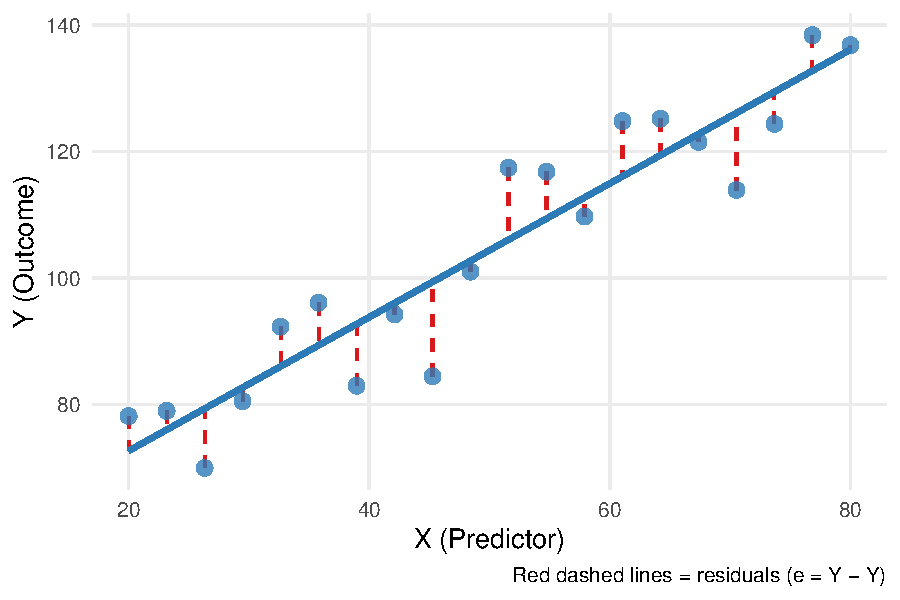
\includegraphics[keepaspectratio]{chapter06_statistical_modeling_files/figure-pdf/fig-ols-1.pdf}}

}

\caption{\label{fig-ols}Least squares regression line minimizes the sum
of squared residuals (vertical red lines)}

\end{figure}%

\begin{center}\rule{0.5\linewidth}{0.5pt}\end{center}

\section{\texorpdfstring{The Coefficient of Determination
(\(R^2\))}{The Coefficient of Determination (R\^{}2)}}\label{the-coefficient-of-determination-r2}

\textbf{\(R^2\)} (R-squared) measures how well the regression line fits
the data --- specifically, the \textbf{proportion of the total variation
in \(Y\) that is explained by \(X\)}:

\[R^2 = r^2 \quad \text{(in simple linear regression)}\]

\[R^2 = \frac{\text{Variation explained by the model}}{\text{Total variation in } Y}\]

\begin{itemize}
\tightlist
\item
  \(R^2 = 1\): the model explains 100\% of the variation in \(Y\)
  (perfect fit)
\item
  \(R^2 = 0\): the model explains none of the variation in \(Y\)
\item
  \(R^2 = 0.65\) means: \emph{``65\% of the variation in \(Y\) is
  explained by \(X\)''}
\end{itemize}

\begin{center}\rule{0.5\linewidth}{0.5pt}\end{center}

\section{Testing the Significance of the
Regression}\label{testing-the-significance-of-the-regression}

Before using the regression equation for interpretation or prediction,
we should test whether the slope \(b_1\) is significantly different from
zero. If \(b_1 = 0\), then \(X\) provides no information about \(Y\).

\textbf{Hypotheses:}

\[H_0: \beta_1 = 0 \quad \text{(X is not a useful predictor of Y)}\]
\[H_1: \beta_1 \neq 0 \quad \text{(X is a useful predictor of Y)}\]

The test statistic is:

\[t = \frac{b_1}{SE_{b_1}}\]

which follows a t-distribution with \(df = n - 2\).

SPSS reports this p-value automatically in the \textbf{Coefficients
table} of the regression output.

\begin{center}\rule{0.5\linewidth}{0.5pt}\end{center}

\section{Assumptions of Linear
Regression}\label{assumptions-of-linear-regression}

The regression model is valid only when the following assumptions are
met:

\begin{Shaded}
\begin{Highlighting}[]
\NormalTok{assump }\OtherTok{\textless{}{-}} \FunctionTok{data.frame}\NormalTok{(}
  \AttributeTok{Assumption =} \FunctionTok{c}\NormalTok{(}\StringTok{"Linearity"}\NormalTok{,}
                 \StringTok{"Independence"}\NormalTok{,}
                 \StringTok{"Homoscedasticity"}\NormalTok{,}
                 \StringTok{"Normality of residuals"}\NormalTok{),}
  \AttributeTok{Meaning =} \FunctionTok{c}\NormalTok{(}
    \StringTok{"The relationship between X and Y is linear (a straight line is appropriate)"}\NormalTok{,}
    \StringTok{"Observations are independent of each other"}\NormalTok{,}
    \StringTok{"The spread of residuals is roughly constant across all values of X"}\NormalTok{,}
    \StringTok{"Residuals are approximately normally distributed"}
\NormalTok{  ),}
  \StringTok{\textasciigrave{}}\AttributeTok{How to Check}\StringTok{\textasciigrave{}} \OtherTok{=} \FunctionTok{c}\NormalTok{(}
    \StringTok{"Scatter plot of X vs. Y; residual plot"}\NormalTok{,}
    \StringTok{"Study design — satisfied by random sampling"}\NormalTok{,}
    \StringTok{"Plot of residuals vs. fitted values — no funnel shape"}\NormalTok{,}
    \StringTok{"Histogram or Q{-}Q plot of residuals"}
\NormalTok{  )}
\NormalTok{)}

\FunctionTok{kable}\NormalTok{(assump, }\AttributeTok{col.names =} \FunctionTok{c}\NormalTok{(}\StringTok{"Assumption"}\NormalTok{, }\StringTok{"Meaning"}\NormalTok{, }\StringTok{"How to Check"}\NormalTok{),}
      \AttributeTok{align =} \FunctionTok{c}\NormalTok{(}\StringTok{"l"}\NormalTok{,}\StringTok{"l"}\NormalTok{,}\StringTok{"l"}\NormalTok{)) }\SpecialCharTok{|\textgreater{}}
  \FunctionTok{kable\_styling}\NormalTok{(}\AttributeTok{bootstrap\_options =} \FunctionTok{c}\NormalTok{(}\StringTok{"striped"}\NormalTok{,}\StringTok{"hover"}\NormalTok{,}\StringTok{"bordered"}\NormalTok{),}
                \AttributeTok{full\_width =} \ConstantTok{TRUE}\NormalTok{, }\AttributeTok{font\_size =} \DecValTok{13}\NormalTok{) }\SpecialCharTok{|\textgreater{}}
  \FunctionTok{column\_spec}\NormalTok{(}\DecValTok{1}\NormalTok{, }\AttributeTok{bold =} \ConstantTok{TRUE}\NormalTok{, }\AttributeTok{color =} \StringTok{"\#2c7bb6"}\NormalTok{)}
\end{Highlighting}
\end{Shaded}

\begin{table}

\caption{\label{tbl-assumptions}Assumptions of Simple Linear Regression}

\centering{

\begingroup\fontsize{13}{15}\selectfont

\begin{longtabu} to \linewidth {>{}l>{\raggedright}X>{\raggedright}X}
\toprule
Assumption & Meaning & How to Check\\
\midrule
\textcolor[HTML]{2c7bb6}{\textbf{Linearity}} & The relationship between X and Y is linear (a straight line is appropriate) & Scatter plot of X vs. Y; residual plot\\
\textcolor[HTML]{2c7bb6}{\textbf{Independence}} & Observations are independent of each other & Study design — satisfied by random sampling\\
\textcolor[HTML]{2c7bb6}{\textbf{Homoscedasticity}} & The spread of residuals is roughly constant across all values of X & Plot of residuals vs. fitted values — no funnel shape\\
\textcolor[HTML]{2c7bb6}{\textbf{Normality of residuals}} & Residuals are approximately normally distributed & Histogram or Q-Q plot of residuals\\
\bottomrule
\end{longtabu}
\endgroup{}

}

\end{table}%

\begin{center}\rule{0.5\linewidth}{0.5pt}\end{center}

\section{Reading SPSS Regression
Output}\label{reading-spss-regression-output}

SPSS produces three key tables for simple linear regression. Here is how
to read them:

\begin{Shaded}
\begin{Highlighting}[]
\NormalTok{model\_sum }\OtherTok{\textless{}{-}} \FunctionTok{data.frame}\NormalTok{(}
  \AttributeTok{R =} \StringTok{"0.821"}\NormalTok{,}
  \AttributeTok{R2 =} \StringTok{"0.674"}\NormalTok{,}
  \StringTok{\textasciigrave{}}\AttributeTok{Adjusted R²}\StringTok{\textasciigrave{}} \OtherTok{=} \StringTok{"0.666"}\NormalTok{,}
  \StringTok{\textasciigrave{}}\AttributeTok{Std. Error of the Estimate}\StringTok{\textasciigrave{}} \OtherTok{=} \StringTok{"8.432"}
\NormalTok{)}

\FunctionTok{kable}\NormalTok{(model\_sum,}
      \AttributeTok{col.names =} \FunctionTok{c}\NormalTok{(}\StringTok{"R"}\NormalTok{, }\StringTok{"R²"}\NormalTok{, }\StringTok{"Adjusted R²"}\NormalTok{, }\StringTok{"Std. Error of the Estimate"}\NormalTok{),}
      \AttributeTok{align =} \FunctionTok{rep}\NormalTok{(}\StringTok{"c"}\NormalTok{,}\DecValTok{4}\NormalTok{)) }\SpecialCharTok{|\textgreater{}}
  \FunctionTok{kable\_styling}\NormalTok{(}\AttributeTok{bootstrap\_options =} \FunctionTok{c}\NormalTok{(}\StringTok{"bordered"}\NormalTok{),}
                \AttributeTok{full\_width =} \ConstantTok{FALSE}\NormalTok{, }\AttributeTok{font\_size =} \DecValTok{13}\NormalTok{) }\SpecialCharTok{|\textgreater{}}
  \FunctionTok{row\_spec}\NormalTok{(}\DecValTok{0}\NormalTok{, }\AttributeTok{bold =} \ConstantTok{TRUE}\NormalTok{, }\AttributeTok{color =} \StringTok{"white"}\NormalTok{, }\AttributeTok{background =} \StringTok{"\#2c7bb6"}\NormalTok{)}
\end{Highlighting}
\end{Shaded}

\begingroup\fontsize{13}{15}\selectfont

\begin{longtable}[t]{cccc}

\caption{\label{tbl-spss-model}SPSS Output: Model Summary}

\tabularnewline

\toprule
\cellcolor[HTML]{2c7bb6}{\textcolor{white}{\textbf{R}}} & \cellcolor[HTML]{2c7bb6}{\textcolor{white}{\textbf{R²}}} & \cellcolor[HTML]{2c7bb6}{\textcolor{white}{\textbf{Adjusted R²}}} & \cellcolor[HTML]{2c7bb6}{\textcolor{white}{\textbf{Std. Error of the Estimate}}}\\
\midrule
0.821 & 0.674 & 0.666 & 8.432\\
\bottomrule

\end{longtable}

\endgroup{}

→ \textbf{R = 0.821} (strong positive correlation); \textbf{R² = 0.674}
(67.4\% of variation in Y explained by X).

\begin{Shaded}
\begin{Highlighting}[]
\NormalTok{anova\_tab }\OtherTok{\textless{}{-}} \FunctionTok{data.frame}\NormalTok{(}
  \AttributeTok{Source =} \FunctionTok{c}\NormalTok{(}\StringTok{"Regression"}\NormalTok{, }\StringTok{"Residual"}\NormalTok{, }\StringTok{"Total"}\NormalTok{),}
  \AttributeTok{SS =} \FunctionTok{c}\NormalTok{(}\StringTok{"5621.4"}\NormalTok{, }\StringTok{"2718.6"}\NormalTok{, }\StringTok{"8340.0"}\NormalTok{),}
  \AttributeTok{df =} \FunctionTok{c}\NormalTok{(}\StringTok{"1"}\NormalTok{, }\StringTok{"38"}\NormalTok{, }\StringTok{"39"}\NormalTok{),}
  \AttributeTok{MS =} \FunctionTok{c}\NormalTok{(}\StringTok{"5621.4"}\NormalTok{, }\StringTok{"71.5"}\NormalTok{, }\StringTok{""}\NormalTok{),}
  \AttributeTok{F =} \FunctionTok{c}\NormalTok{(}\StringTok{"78.62"}\NormalTok{, }\StringTok{""}\NormalTok{, }\StringTok{""}\NormalTok{),}
  \AttributeTok{Sig =} \FunctionTok{c}\NormalTok{(}\StringTok{"\textless{} 0.001"}\NormalTok{, }\StringTok{""}\NormalTok{, }\StringTok{""}\NormalTok{)}
\NormalTok{)}

\FunctionTok{kable}\NormalTok{(anova\_tab,}
      \AttributeTok{col.names =} \FunctionTok{c}\NormalTok{(}\StringTok{""}\NormalTok{, }\StringTok{"Sum of Squares"}\NormalTok{, }\StringTok{"df"}\NormalTok{, }\StringTok{"Mean Square"}\NormalTok{, }\StringTok{"F"}\NormalTok{, }\StringTok{"Sig."}\NormalTok{),}
      \AttributeTok{align =} \FunctionTok{c}\NormalTok{(}\StringTok{"l"}\NormalTok{,}\StringTok{"c"}\NormalTok{,}\StringTok{"c"}\NormalTok{,}\StringTok{"c"}\NormalTok{,}\StringTok{"c"}\NormalTok{,}\StringTok{"c"}\NormalTok{)) }\SpecialCharTok{|\textgreater{}}
  \FunctionTok{kable\_styling}\NormalTok{(}\AttributeTok{bootstrap\_options =} \FunctionTok{c}\NormalTok{(}\StringTok{"bordered"}\NormalTok{),}
                \AttributeTok{full\_width =} \ConstantTok{FALSE}\NormalTok{, }\AttributeTok{font\_size =} \DecValTok{13}\NormalTok{) }\SpecialCharTok{|\textgreater{}}
  \FunctionTok{row\_spec}\NormalTok{(}\DecValTok{0}\NormalTok{, }\AttributeTok{bold =} \ConstantTok{TRUE}\NormalTok{, }\AttributeTok{color =} \StringTok{"white"}\NormalTok{, }\AttributeTok{background =} \StringTok{"\#2c7bb6"}\NormalTok{) }\SpecialCharTok{|\textgreater{}}
  \FunctionTok{row\_spec}\NormalTok{(}\DecValTok{1}\NormalTok{, }\AttributeTok{bold =} \ConstantTok{TRUE}\NormalTok{)}
\end{Highlighting}
\end{Shaded}

\begingroup\fontsize{13}{15}\selectfont

\begin{longtable}[t]{lccccc}

\caption{\label{tbl-spss-anova}SPSS Output: ANOVA Table}

\tabularnewline

\toprule
\cellcolor[HTML]{2c7bb6}{\textcolor{white}{\textbf{}}} & \cellcolor[HTML]{2c7bb6}{\textcolor{white}{\textbf{Sum of Squares}}} & \cellcolor[HTML]{2c7bb6}{\textcolor{white}{\textbf{df}}} & \cellcolor[HTML]{2c7bb6}{\textcolor{white}{\textbf{Mean Square}}} & \cellcolor[HTML]{2c7bb6}{\textcolor{white}{\textbf{F}}} & \cellcolor[HTML]{2c7bb6}{\textcolor{white}{\textbf{Sig.}}}\\
\midrule
\textbf{Regression} & \textbf{5621.4} & \textbf{1} & \textbf{5621.4} & \textbf{78.62} & \textbf{< 0.001}\\
Residual & 2718.6 & 38 & 71.5 &  & \\
Total & 8340.0 & 39 &  &  & \\
\bottomrule

\end{longtable}

\endgroup{}

→ \textbf{F = 78.62, p \textless{} 0.001} --- the overall regression
model is statistically significant.

\begin{Shaded}
\begin{Highlighting}[]
\NormalTok{coef\_tab }\OtherTok{\textless{}{-}} \FunctionTok{data.frame}\NormalTok{(}
  \StringTok{\textasciigrave{}}\AttributeTok{ }\StringTok{\textasciigrave{}} \OtherTok{=} \FunctionTok{c}\NormalTok{(}\StringTok{"(Constant)"}\NormalTok{, }\StringTok{"X (predictor)"}\NormalTok{),}
  \AttributeTok{B =} \FunctionTok{c}\NormalTok{(}\StringTok{"32.15"}\NormalTok{, }\StringTok{"0.87"}\NormalTok{),}
  \AttributeTok{SE =} \FunctionTok{c}\NormalTok{(}\StringTok{"6.24"}\NormalTok{, }\StringTok{"0.10"}\NormalTok{),}
  \AttributeTok{Beta =} \FunctionTok{c}\NormalTok{(}\StringTok{"—"}\NormalTok{, }\StringTok{"0.821"}\NormalTok{),}
  \AttributeTok{t =} \FunctionTok{c}\NormalTok{(}\StringTok{"5.15"}\NormalTok{, }\StringTok{"8.87"}\NormalTok{),}
  \AttributeTok{Sig =} \FunctionTok{c}\NormalTok{(}\StringTok{"\textless{} 0.001"}\NormalTok{, }\StringTok{"\textless{} 0.001"}\NormalTok{)}
\NormalTok{)}

\FunctionTok{kable}\NormalTok{(coef\_tab,}
      \AttributeTok{col.names =} \FunctionTok{c}\NormalTok{(}\StringTok{""}\NormalTok{, }\StringTok{"B"}\NormalTok{, }\StringTok{"Std. Error"}\NormalTok{, }\StringTok{"Beta (standardized)"}\NormalTok{, }\StringTok{"t"}\NormalTok{, }\StringTok{"Sig."}\NormalTok{),}
      \AttributeTok{align =} \FunctionTok{c}\NormalTok{(}\StringTok{"l"}\NormalTok{,}\StringTok{"c"}\NormalTok{,}\StringTok{"c"}\NormalTok{,}\StringTok{"c"}\NormalTok{,}\StringTok{"c"}\NormalTok{,}\StringTok{"c"}\NormalTok{)) }\SpecialCharTok{|\textgreater{}}
  \FunctionTok{kable\_styling}\NormalTok{(}\AttributeTok{bootstrap\_options =} \FunctionTok{c}\NormalTok{(}\StringTok{"bordered"}\NormalTok{),}
                \AttributeTok{full\_width =} \ConstantTok{FALSE}\NormalTok{, }\AttributeTok{font\_size =} \DecValTok{13}\NormalTok{) }\SpecialCharTok{|\textgreater{}}
  \FunctionTok{row\_spec}\NormalTok{(}\DecValTok{0}\NormalTok{, }\AttributeTok{bold =} \ConstantTok{TRUE}\NormalTok{, }\AttributeTok{color =} \StringTok{"white"}\NormalTok{, }\AttributeTok{background =} \StringTok{"\#2c7bb6"}\NormalTok{) }\SpecialCharTok{|\textgreater{}}
  \FunctionTok{row\_spec}\NormalTok{(}\DecValTok{2}\NormalTok{, }\AttributeTok{bold =} \ConstantTok{TRUE}\NormalTok{, }\AttributeTok{background =} \StringTok{"\#eaf4fb"}\NormalTok{)}
\end{Highlighting}
\end{Shaded}

\begingroup\fontsize{13}{15}\selectfont

\begin{longtable}[t]{lccccc}

\caption{\label{tbl-spss-coef}SPSS Output: Coefficients Table}

\tabularnewline

\toprule
\cellcolor[HTML]{2c7bb6}{\textcolor{white}{\textbf{}}} & \cellcolor[HTML]{2c7bb6}{\textcolor{white}{\textbf{B}}} & \cellcolor[HTML]{2c7bb6}{\textcolor{white}{\textbf{Std. Error}}} & \cellcolor[HTML]{2c7bb6}{\textcolor{white}{\textbf{Beta (standardized)}}} & \cellcolor[HTML]{2c7bb6}{\textcolor{white}{\textbf{t}}} & \cellcolor[HTML]{2c7bb6}{\textcolor{white}{\textbf{Sig.}}}\\
\midrule
(Constant) & 32.15 & 6.24 & — & 5.15 & < 0.001\\
\cellcolor[HTML]{eaf4fb}{\textbf{X (predictor)}} & \cellcolor[HTML]{eaf4fb}{\textbf{0.87}} & \cellcolor[HTML]{eaf4fb}{\textbf{0.10}} & \cellcolor[HTML]{eaf4fb}{\textbf{0.821}} & \cellcolor[HTML]{eaf4fb}{\textbf{8.87}} & \cellcolor[HTML]{eaf4fb}{\textbf{< 0.001}}\\
\bottomrule

\end{longtable}

\endgroup{}

→ \textbf{Regression equation:} \(\hat{Y} = 32.15 + 0.87X\)

→ The slope \textbf{B = 0.87} is statistically significant
(\(p < 0.001\)): for each one-unit increase in \(X\), \(Y\) increases by
\textbf{0.87 units} on average.

\begin{center}\rule{0.5\linewidth}{0.5pt}\end{center}

\bookmarksetup{startatroot}

\chapter{Key Takeaways}\label{key-takeaways-5}

\begin{tcolorbox}[enhanced jigsaw, arc=.35mm, bottomrule=.15mm, bottomtitle=1mm, breakable, colback=white, colbacktitle=quarto-callout-note-color!10!white, colframe=quarto-callout-note-color-frame, coltitle=black, left=2mm, leftrule=.75mm, opacityback=0, opacitybacktitle=0.6, rightrule=.15mm, title={📝 Chapter 6 Summary}, titlerule=0mm, toprule=.15mm, toptitle=1mm]

\begin{enumerate}
\def\labelenumi{\arabic{enumi}.}
\item
  \textbf{Statistical modeling} describes the mathematical relationship
  between an outcome variable \(Y\) and one or more predictor variables
  \(X\).
\item
  \textbf{Pearson's \(r\)} measures the strength and direction of a
  linear relationship between two continuous variables
  (\(-1 \leq r \leq +1\)).
\item
  \textbf{Simple linear regression} fits the equation
  \(\hat{Y} = b_0 + b_1 X\) using the least squares method, which
  minimizes the sum of squared residuals.
\item
  The \textbf{slope \(b_1\)} tells us how much \(Y\) changes for each
  one-unit increase in \(X\); the \textbf{intercept \(b_0\)} is the
  predicted value of \(Y\) when \(X = 0\).
\item
  \textbf{\(R^2\)} is the proportion of variation in \(Y\) explained by
  the model. A higher \(R^2\) means a better fit.
\item
  Always test whether \(b_1\) is significantly different from zero
  (\(H_0: \beta_1 = 0\)) before using the model for interpretation.
\item
  The model is only valid when the four assumptions ---
  \textbf{linearity, independence, homoscedasticity, and normality of
  residuals} --- are reasonably satisfied.
\end{enumerate}

\end{tcolorbox}

\begin{center}\rule{0.5\linewidth}{0.5pt}\end{center}

\bookmarksetup{startatroot}

\chapter{Examples}\label{examples-5}

\section{Example 1: Calculating Correlation and
Regression}\label{example-1-calculating-correlation-and-regression}

A researcher records the \textbf{age (years)} and \textbf{systolic blood
pressure (mmHg)} of 8 adults:

\begin{Shaded}
\begin{Highlighting}[]
\NormalTok{age }\OtherTok{\textless{}{-}} \FunctionTok{c}\NormalTok{(}\DecValTok{25}\NormalTok{, }\DecValTok{32}\NormalTok{, }\DecValTok{40}\NormalTok{, }\DecValTok{48}\NormalTok{, }\DecValTok{55}\NormalTok{, }\DecValTok{62}\NormalTok{, }\DecValTok{70}\NormalTok{, }\DecValTok{78}\NormalTok{)}
\NormalTok{sbp }\OtherTok{\textless{}{-}} \FunctionTok{c}\NormalTok{(}\DecValTok{115}\NormalTok{, }\DecValTok{120}\NormalTok{, }\DecValTok{128}\NormalTok{, }\DecValTok{135}\NormalTok{, }\DecValTok{142}\NormalTok{, }\DecValTok{148}\NormalTok{, }\DecValTok{158}\NormalTok{, }\DecValTok{165}\NormalTok{)}

\NormalTok{ex1 }\OtherTok{\textless{}{-}} \FunctionTok{data.frame}\NormalTok{(}\AttributeTok{Subject =} \FunctionTok{paste0}\NormalTok{(}\StringTok{"S"}\NormalTok{, }\DecValTok{1}\SpecialCharTok{:}\DecValTok{8}\NormalTok{), }\AttributeTok{Age =}\NormalTok{ age, }\AttributeTok{SBP =}\NormalTok{ sbp)}

\FunctionTok{kable}\NormalTok{(ex1, }\AttributeTok{col.names =} \FunctionTok{c}\NormalTok{(}\StringTok{"Subject"}\NormalTok{, }\StringTok{"Age (years)"}\NormalTok{, }\StringTok{"SBP (mmHg)"}\NormalTok{),}
      \AttributeTok{align =} \FunctionTok{c}\NormalTok{(}\StringTok{"c"}\NormalTok{,}\StringTok{"c"}\NormalTok{,}\StringTok{"c"}\NormalTok{)) }\SpecialCharTok{|\textgreater{}}
  \FunctionTok{kable\_styling}\NormalTok{(}\AttributeTok{bootstrap\_options =} \FunctionTok{c}\NormalTok{(}\StringTok{"striped"}\NormalTok{,}\StringTok{"hover"}\NormalTok{,}\StringTok{"bordered"}\NormalTok{),}
                \AttributeTok{full\_width =} \ConstantTok{FALSE}\NormalTok{, }\AttributeTok{font\_size =} \DecValTok{13}\NormalTok{)}
\end{Highlighting}
\end{Shaded}

\begingroup\fontsize{13}{15}\selectfont

\begin{longtable}[t]{ccc}

\caption{\label{tbl-ex1-data}Age and Systolic Blood Pressure of 8
Adults}

\tabularnewline

\toprule
Subject & Age (years) & SBP (mmHg)\\
\midrule
S1 & 25 & 115\\
S2 & 32 & 120\\
S3 & 40 & 128\\
S4 & 48 & 135\\
S5 & 55 & 142\\
\addlinespace
S6 & 62 & 148\\
S7 & 70 & 158\\
S8 & 78 & 165\\
\bottomrule

\end{longtable}

\endgroup{}

\textbf{(a)} Calculate Pearson's \(r\).

\textbf{(b)} Find the regression equation \(\hat{Y} = b_0 + b_1 X\).

\textbf{(c)} Predict the SBP of a 50-year-old adult.

\textbf{(d)} Interpret \(R^2\).

\begin{tcolorbox}[enhanced jigsaw, arc=.35mm, bottomrule=.15mm, bottomtitle=1mm, breakable, colback=white, colbacktitle=quarto-callout-tip-color!10!white, colframe=quarto-callout-tip-color-frame, coltitle=black, left=2mm, leftrule=.75mm, opacityback=0, opacitybacktitle=0.6, rightrule=.15mm, title={✅ Solution}, titlerule=0mm, toprule=.15mm, toptitle=1mm]

\begin{Shaded}
\begin{Highlighting}[]
\NormalTok{xbar }\OtherTok{\textless{}{-}} \FunctionTok{mean}\NormalTok{(age)}
\NormalTok{ybar }\OtherTok{\textless{}{-}} \FunctionTok{mean}\NormalTok{(sbp)}

\NormalTok{calc }\OtherTok{\textless{}{-}} \FunctionTok{data.frame}\NormalTok{(}
  \AttributeTok{Subject =} \FunctionTok{paste0}\NormalTok{(}\StringTok{"S"}\NormalTok{, }\DecValTok{1}\SpecialCharTok{:}\DecValTok{8}\NormalTok{),}
  \AttributeTok{x =}\NormalTok{ age,}
  \AttributeTok{y =}\NormalTok{ sbp,}
  \AttributeTok{xdev =} \FunctionTok{round}\NormalTok{(age }\SpecialCharTok{{-}}\NormalTok{ xbar, }\DecValTok{2}\NormalTok{),}
  \AttributeTok{ydev =} \FunctionTok{round}\NormalTok{(sbp }\SpecialCharTok{{-}}\NormalTok{ ybar, }\DecValTok{2}\NormalTok{),}
  \AttributeTok{xdev2 =} \FunctionTok{round}\NormalTok{((age }\SpecialCharTok{{-}}\NormalTok{ xbar)}\SpecialCharTok{\^{}}\DecValTok{2}\NormalTok{, }\DecValTok{2}\NormalTok{),}
  \AttributeTok{ydev2 =} \FunctionTok{round}\NormalTok{((sbp }\SpecialCharTok{{-}}\NormalTok{ ybar)}\SpecialCharTok{\^{}}\DecValTok{2}\NormalTok{, }\DecValTok{2}\NormalTok{),}
  \AttributeTok{xydev =} \FunctionTok{round}\NormalTok{((age }\SpecialCharTok{{-}}\NormalTok{ xbar)}\SpecialCharTok{*}\NormalTok{(sbp }\SpecialCharTok{{-}}\NormalTok{ ybar), }\DecValTok{2}\NormalTok{)}
\NormalTok{)}

\NormalTok{totrow }\OtherTok{\textless{}{-}} \FunctionTok{data.frame}\NormalTok{(}
  \AttributeTok{Subject =} \StringTok{"**Total**"}\NormalTok{,}
  \AttributeTok{x =} \ConstantTok{NA}\NormalTok{, }\AttributeTok{y =} \ConstantTok{NA}\NormalTok{,}
  \AttributeTok{xdev =} \ConstantTok{NA}\NormalTok{, }\AttributeTok{ydev =} \ConstantTok{NA}\NormalTok{,}
  \AttributeTok{xdev2 =} \FunctionTok{round}\NormalTok{(}\FunctionTok{sum}\NormalTok{((age}\SpecialCharTok{{-}}\NormalTok{xbar)}\SpecialCharTok{\^{}}\DecValTok{2}\NormalTok{), }\DecValTok{2}\NormalTok{),}
  \AttributeTok{ydev2 =} \FunctionTok{round}\NormalTok{(}\FunctionTok{sum}\NormalTok{((sbp}\SpecialCharTok{{-}}\NormalTok{ybar)}\SpecialCharTok{\^{}}\DecValTok{2}\NormalTok{), }\DecValTok{2}\NormalTok{),}
  \AttributeTok{xydev =} \FunctionTok{round}\NormalTok{(}\FunctionTok{sum}\NormalTok{((age}\SpecialCharTok{{-}}\NormalTok{xbar)}\SpecialCharTok{*}\NormalTok{(sbp}\SpecialCharTok{{-}}\NormalTok{ybar)), }\DecValTok{2}\NormalTok{)}
\NormalTok{)}

\NormalTok{calc\_all }\OtherTok{\textless{}{-}} \FunctionTok{rbind}\NormalTok{(calc, totrow)}

\FunctionTok{kable}\NormalTok{(calc\_all,}
      \AttributeTok{col.names =} \FunctionTok{c}\NormalTok{(}\StringTok{"Subject"}\NormalTok{,}\StringTok{"x"}\NormalTok{,}\StringTok{"y"}\NormalTok{,}\StringTok{"x−x̄"}\NormalTok{,}\StringTok{"y−ȳ"}\NormalTok{,}
                    \StringTok{"(x−x̄)²"}\NormalTok{,}\StringTok{"(y−ȳ)²"}\NormalTok{,}\StringTok{"(x−x̄)(y−ȳ)"}\NormalTok{),}
      \AttributeTok{align =} \FunctionTok{rep}\NormalTok{(}\StringTok{"c"}\NormalTok{, }\DecValTok{8}\NormalTok{), }\AttributeTok{escape =} \ConstantTok{FALSE}\NormalTok{, }\AttributeTok{na\_print =} \StringTok{"—"}\NormalTok{) }\SpecialCharTok{|\textgreater{}}
  \FunctionTok{kable\_styling}\NormalTok{(}\AttributeTok{bootstrap\_options =} \FunctionTok{c}\NormalTok{(}\StringTok{"striped"}\NormalTok{,}\StringTok{"hover"}\NormalTok{,}\StringTok{"bordered"}\NormalTok{),}
                \AttributeTok{full\_width =} \ConstantTok{TRUE}\NormalTok{, }\AttributeTok{font\_size =} \DecValTok{12}\NormalTok{) }\SpecialCharTok{|\textgreater{}}
  \FunctionTok{row\_spec}\NormalTok{(}\DecValTok{9}\NormalTok{, }\AttributeTok{bold =} \ConstantTok{TRUE}\NormalTok{, }\AttributeTok{background =} \StringTok{"\#eaf4fb"}\NormalTok{) }\SpecialCharTok{|\textgreater{}}
  \FunctionTok{row\_spec}\NormalTok{(}\DecValTok{0}\NormalTok{, }\AttributeTok{bold =} \ConstantTok{TRUE}\NormalTok{, }\AttributeTok{color =} \StringTok{"white"}\NormalTok{, }\AttributeTok{background =} \StringTok{"\#2c7bb6"}\NormalTok{)}
\end{Highlighting}
\end{Shaded}

\begin{table}[H]

\caption{\label{tbl-ex1-calc}Calculation Table for Correlation and
Regression}

\centering{

\begingroup\fontsize{12}{14}\selectfont

\begin{longtabu} to \linewidth {>{\centering}X>{\centering}X>{\centering}X>{\centering}X>{\centering}X>{\centering}X>{\centering}X>{\centering}X}
\toprule
\cellcolor[HTML]{2c7bb6}{\textcolor{white}{\textbf{Subject}}} & \cellcolor[HTML]{2c7bb6}{\textcolor{white}{\textbf{x}}} & \cellcolor[HTML]{2c7bb6}{\textcolor{white}{\textbf{y}}} & \cellcolor[HTML]{2c7bb6}{\textcolor{white}{\textbf{x−x̄}}} & \cellcolor[HTML]{2c7bb6}{\textcolor{white}{\textbf{|  y−ȳ}}} & \cellcolor[HTML]{2c7bb6}{\textcolor{white}{\textbf{| (x−x̄)²}}} & \cellcolor[HTML]{2c7bb6}{\textcolor{white}{\textbf{| (y−ȳ)²}}} & \cellcolor[HTML]{2c7bb6}{\textcolor{white}{\textbf{| (x−x̄)(y−}}}\\
\midrule
S1 & 25 & 115 & -26.25 & -23.88 & 689.06 & 570.02 & 626.72\\
S2 & 32 & 120 & -19.25 & -18.88 & 370.56 & 356.27 & 363.34\\
S3 & 40 & 128 & -11.25 & -10.88 & 126.56 & 118.27 & 122.34\\
S4 & 48 & 135 & -3.25 & -3.88 & 10.56 & 15.02 & 12.59\\
S5 & 55 & 142 & 3.75 & 3.12 & 14.06 & 9.77 & 11.72\\
\addlinespace
S6 & 62 & 148 & 10.75 & 9.12 & 115.56 & 83.27 & 98.09\\
S7 & 70 & 158 & 18.75 & 19.12 & 351.56 & 365.77 & 358.59\\
S8 & 78 & 165 & 26.75 & 26.12 & 715.56 & 682.52 & 698.84\\
\cellcolor[HTML]{eaf4fb}{\textbf{**Total**}} & \cellcolor[HTML]{eaf4fb}{\textbf{NA}} & \cellcolor[HTML]{eaf4fb}{\textbf{NA}} & \cellcolor[HTML]{eaf4fb}{\textbf{NA}} & \cellcolor[HTML]{eaf4fb}{\textbf{NA}} & \cellcolor[HTML]{eaf4fb}{\textbf{2393.50}} & \cellcolor[HTML]{eaf4fb}{\textbf{2200.88}} & \cellcolor[HTML]{eaf4fb}{\textbf{2292.25}}\\
\bottomrule
\end{longtabu}
\endgroup{}

}

\end{table}%

\textbf{(a) Pearson's r:}

\[r = \frac{\sum(x_i-\bar{x})(y_i-\bar{y})}
           {\sqrt{\sum(x_i-\bar{x})^2 \cdot \sum(y_i-\bar{y})^2}}
  = \frac{2292.25}
         {\sqrt{2393.5 \times 2200.88}}
  = \frac{2292.25}
         {2295.17}
  = \mathbf{0.999}\]

This indicates a \textbf{very strong positive} linear relationship
between age and systolic blood pressure.

\textbf{(b) Regression coefficients:}

\[b_1 = \frac{\sum(x_i-\bar{x})(y_i-\bar{y})}{\sum(x_i-\bar{x})^2}
      = \frac{2292.25}
             {2393.5}
      = 0.958\]

\[b_0 = \bar{y} - b_1\bar{x}
      = 138.88 - 0.958 \times 51.25
      = 89.79\]

\[\boxed{\hat{Y} = 89.79 + 0.958 X}\]

\textbf{(c) Prediction for age = 50:}

\[\hat{Y} = 89.79 + 0.958 \times 50
          = 137.7 \text{ mmHg}\]

\textbf{(d) \(R^2\):}

\[R^2 = r^2 = (0.999)^2 = 0.997\]

\textbf{99.7\% of the variation in systolic blood pressure is explained
by age.} The remaining 0.3\% is due to other factors not included in
this model.

\end{tcolorbox}

\begin{Shaded}
\begin{Highlighting}[]
\NormalTok{fit1 }\OtherTok{\textless{}{-}} \FunctionTok{lm}\NormalTok{(sbp }\SpecialCharTok{\textasciitilde{}}\NormalTok{ age)}
\NormalTok{df1  }\OtherTok{\textless{}{-}} \FunctionTok{data.frame}\NormalTok{(}\AttributeTok{age =}\NormalTok{ age, }\AttributeTok{sbp =}\NormalTok{ sbp)}

\FunctionTok{ggplot}\NormalTok{(df1, }\FunctionTok{aes}\NormalTok{(}\AttributeTok{x =}\NormalTok{ age, }\AttributeTok{y =}\NormalTok{ sbp)) }\SpecialCharTok{+}
  \FunctionTok{geom\_point}\NormalTok{(}\AttributeTok{size =} \FloatTok{3.5}\NormalTok{, }\AttributeTok{color =} \StringTok{"\#2c7bb6"}\NormalTok{) }\SpecialCharTok{+}
  \FunctionTok{geom\_smooth}\NormalTok{(}\AttributeTok{method =} \StringTok{"lm"}\NormalTok{, }\AttributeTok{se =} \ConstantTok{TRUE}\NormalTok{, }\AttributeTok{color =} \StringTok{"\#d7191c"}\NormalTok{,}
              \AttributeTok{fill =} \StringTok{"\#fdae61"}\NormalTok{, }\AttributeTok{alpha =} \FloatTok{0.2}\NormalTok{, }\AttributeTok{formula =}\NormalTok{ y }\SpecialCharTok{\textasciitilde{}}\NormalTok{ x) }\SpecialCharTok{+}
  \FunctionTok{annotate}\NormalTok{(}\StringTok{"text"}\NormalTok{, }\AttributeTok{x =} \DecValTok{30}\NormalTok{, }\AttributeTok{y =} \DecValTok{162}\NormalTok{,}
           \AttributeTok{label =} \FunctionTok{paste0}\NormalTok{(}\StringTok{"Ŷ = "}\NormalTok{, }\FunctionTok{round}\NormalTok{(}\FunctionTok{coef}\NormalTok{(fit1)[}\DecValTok{1}\NormalTok{],}\DecValTok{2}\NormalTok{),}
                          \StringTok{" + "}\NormalTok{, }\FunctionTok{round}\NormalTok{(}\FunctionTok{coef}\NormalTok{(fit1)[}\DecValTok{2}\NormalTok{],}\DecValTok{3}\NormalTok{), }\StringTok{"X}\SpecialCharTok{\textbackslash{}n}\StringTok{"}\NormalTok{,}
                          \StringTok{"r = "}\NormalTok{, }\FunctionTok{round}\NormalTok{(}\FunctionTok{cor}\NormalTok{(age,sbp),}\DecValTok{3}\NormalTok{),}
                          \StringTok{",  R² = "}\NormalTok{, }\FunctionTok{round}\NormalTok{(}\FunctionTok{cor}\NormalTok{(age,sbp)}\SpecialCharTok{\^{}}\DecValTok{2}\NormalTok{,}\DecValTok{3}\NormalTok{)),}
           \AttributeTok{hjust =} \DecValTok{0}\NormalTok{, }\AttributeTok{size =} \DecValTok{4}\NormalTok{, }\AttributeTok{color =} \StringTok{"\#d7191c"}\NormalTok{) }\SpecialCharTok{+}
  \FunctionTok{labs}\NormalTok{(}\AttributeTok{x =} \StringTok{"Age (years)"}\NormalTok{, }\AttributeTok{y =} \StringTok{"Systolic Blood Pressure (mmHg)"}\NormalTok{) }\SpecialCharTok{+}
  \FunctionTok{theme\_minimal}\NormalTok{(}\AttributeTok{base\_size =} \DecValTok{13}\NormalTok{) }\SpecialCharTok{+}
  \FunctionTok{theme}\NormalTok{(}\AttributeTok{panel.grid.minor =} \FunctionTok{element\_blank}\NormalTok{())}
\end{Highlighting}
\end{Shaded}

\begin{figure}[H]

\centering{

\pandocbounded{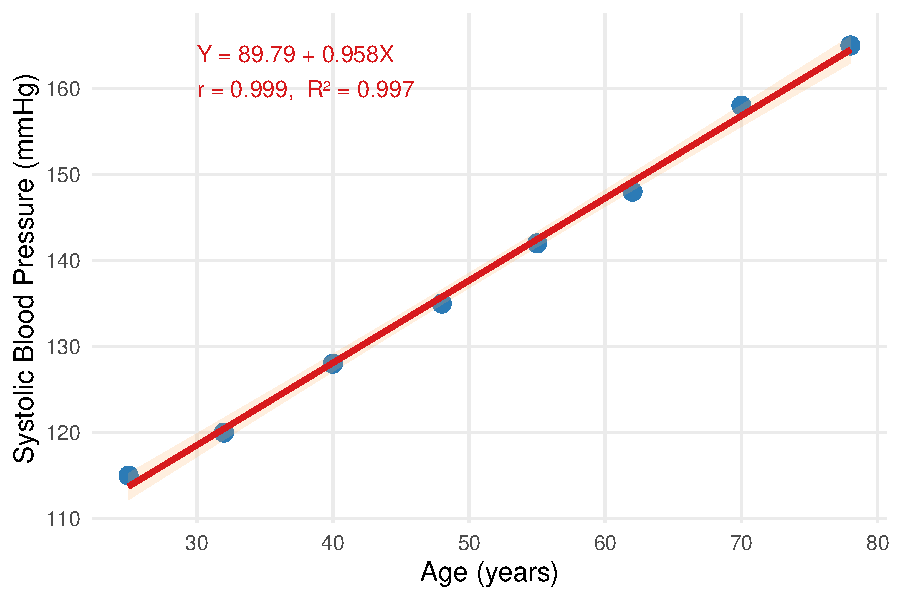
\includegraphics[keepaspectratio]{chapter06_statistical_modeling_files/figure-pdf/fig-ex1-fit-1.pdf}}

}

\caption{\label{fig-ex1-fit}Scatter plot with fitted regression line:
Age vs.~Systolic Blood Pressure}

\end{figure}%

\begin{center}\rule{0.5\linewidth}{0.5pt}\end{center}

\section{Example 2: Interpreting SPSS
Output}\label{example-2-interpreting-spss-output}

A researcher uses SPSS to examine the relationship between \textbf{BMI
(kg/m²)} and \textbf{fasting blood glucose (mg/dL)} in 60 adults. The
following output is obtained:

\textbf{Model Summary:}

{\def\LTcaptype{none} % do not increment counter
\begin{longtable}[]{@{}cccc@{}}
\toprule\noalign{}
R & R² & Adjusted R² & Std. Error \\
\midrule\noalign{}
\endhead
\bottomrule\noalign{}
\endlastfoot
0.612 & 0.375 & 0.364 & 14.23 \\
\end{longtable}
}

\textbf{Coefficients:}

{\def\LTcaptype{none} % do not increment counter
\begin{longtable}[]{@{}lcccc@{}}
\toprule\noalign{}
& B & Std. Error & t & Sig. \\
\midrule\noalign{}
\endhead
\bottomrule\noalign{}
\endlastfoot
(Constant) & 48.32 & 11.45 & 4.22 & \textless{} 0.001 \\
BMI & 2.91 & 0.46 & 6.33 & \textless{} 0.001 \\
\end{longtable}
}

\begin{tcolorbox}[enhanced jigsaw, arc=.35mm, bottomrule=.15mm, bottomtitle=1mm, breakable, colback=white, colbacktitle=quarto-callout-tip-color!10!white, colframe=quarto-callout-tip-color-frame, coltitle=black, left=2mm, leftrule=.75mm, opacityback=0, opacitybacktitle=0.6, rightrule=.15mm, title={✅ Interpretation}, titlerule=0mm, toprule=.15mm, toptitle=1mm]

\textbf{Correlation:} \(r = 0.612\) --- a \textbf{moderate-to-strong
positive} relationship between BMI and fasting blood glucose.

\textbf{Regression equation:}
\[\hat{Y} = 48.32 + 2.91 \times \text{BMI}\]

\textbf{Slope (\(b_1 = 2.91\)):} For each 1 kg/m² increase in BMI,
fasting blood glucose increases by \textbf{2.91 mg/dL} on average,
holding other factors constant.

\textbf{Intercept (\(b_0 = 48.32\)):} The predicted fasting glucose when
BMI = 0 is 48.32 mg/dL. \emph{(Note: BMI of 0 is not a meaningful value
in practice --- the intercept is simply a mathematical anchor for the
line.)}

\textbf{\(R^2 = 0.375\):} BMI explains \textbf{37.5\%} of the variation
in fasting blood glucose. The remaining 62.5\% is due to other factors
(diet, genetics, physical activity, etc.).

\textbf{Significance (\(p < 0.001\)):} The slope is highly significant
--- BMI is a statistically significant predictor of fasting blood
glucose.

\textbf{Prediction example:} A person with BMI = 28 kg/m²:
\[\hat{Y} = 48.32 + 2.91 \times 28 = 48.32 + 81.48 = 129.8 \text{ mg/dL}\]

\end{tcolorbox}

\begin{center}\rule{0.5\linewidth}{0.5pt}\end{center}

\bookmarksetup{startatroot}

\chapter{Exercises}\label{exercises-5}

\begin{tcolorbox}[enhanced jigsaw, arc=.35mm, bottomrule=.15mm, bottomtitle=1mm, breakable, colback=white, colbacktitle=quarto-callout-caution-color!10!white, colframe=quarto-callout-caution-color-frame, coltitle=black, left=2mm, leftrule=.75mm, opacityback=0, opacitybacktitle=0.6, rightrule=.15mm, title={✏️ Exercise 1}, titlerule=0mm, toprule=.15mm, toptitle=1mm]

A study records the \textbf{hours of sleep per night} (\(X\)) and
\textbf{systolic blood pressure (mmHg)} (\(Y\)) for 6 adults:

{\def\LTcaptype{none} % do not increment counter
\begin{longtable}[]{@{}ccc@{}}
\toprule\noalign{}
Subject & Sleep (hrs) & SBP (mmHg) \\
\midrule\noalign{}
\endhead
\bottomrule\noalign{}
\endlastfoot
1 & 5 & 145 \\
2 & 6 & 138 \\
3 & 7 & 130 \\
4 & 7 & 125 \\
5 & 8 & 120 \\
6 & 9 & 115 \\
\end{longtable}
}

\textbf{(a)} Draw a scatter plot and describe the relationship.

\textbf{(b)} Calculate Pearson's \(r\). What does it indicate?

\textbf{(c)} Find the regression equation \(\hat{Y} = b_0 + b_1 X\).

\textbf{(d)} Predict the SBP of a person who sleeps 6.5 hours per night.

\textbf{(e)} Calculate \(R^2\) and interpret it.

\end{tcolorbox}

\begin{tcolorbox}[enhanced jigsaw, arc=.35mm, bottomrule=.15mm, bottomtitle=1mm, breakable, colback=white, colbacktitle=quarto-callout-caution-color!10!white, colframe=quarto-callout-caution-color-frame, coltitle=black, left=2mm, leftrule=.75mm, opacityback=0, opacitybacktitle=0.6, rightrule=.15mm, title={✏️ Exercise 2}, titlerule=0mm, toprule=.15mm, toptitle=1mm]

A researcher uses SPSS to study the relationship between a patient's
\textbf{age (years)} and \textbf{total cholesterol (mg/dL)}. The SPSS
output gives the following results:

\textbf{Model Summary:} R = 0.548, R² = 0.300

\textbf{Coefficients:}

{\def\LTcaptype{none} % do not increment counter
\begin{longtable}[]{@{}lcccc@{}}
\toprule\noalign{}
& B & Std. Error & t & Sig. \\
\midrule\noalign{}
\endhead
\bottomrule\noalign{}
\endlastfoot
(Constant) & 120.4 & 18.6 & 6.47 & \textless{} 0.001 \\
Age & 1.85 & 0.31 & 5.97 & \textless{} 0.001 \\
\end{longtable}
}

\textbf{(a)} Write the regression equation.

\textbf{(b)} Interpret the slope in the context of this study.

\textbf{(c)} What proportion of the variation in cholesterol is
explained by age? Is this a strong model?

\textbf{(d)} Predict the total cholesterol of a 55-year-old patient.

\textbf{(e)} Is the predictor (age) statistically significant at
\(\alpha = 0.05\)? How do you know?

\end{tcolorbox}

\begin{tcolorbox}[enhanced jigsaw, arc=.35mm, bottomrule=.15mm, bottomtitle=1mm, breakable, colback=white, colbacktitle=quarto-callout-caution-color!10!white, colframe=quarto-callout-caution-color-frame, coltitle=black, left=2mm, leftrule=.75mm, opacityback=0, opacitybacktitle=0.6, rightrule=.15mm, title={✏️ Exercise 3 --- Reflection Questions}, titlerule=0mm, toprule=.15mm, toptitle=1mm]

Answer the following in 2--3 sentences each:

\textbf{(a)} A researcher finds that the correlation between ice cream
sales and drowning deaths is \(r = 0.85\). Does this mean eating ice
cream causes drowning? Explain using the concept of correlation
vs.~causation.

\textbf{(b)} In a regression model predicting patient recovery time from
age (\(R^2 = 0.22\)), a colleague says \emph{``this model is useless
because it only explains 22\% of the variation.''} Do you agree? What
additional information would help evaluate this claim?

\textbf{(c)} Why is it generally not appropriate to use a regression
equation to predict \(Y\) for values of \(X\) that are far outside the
range of the original data?

\end{tcolorbox}

\begin{center}\rule{0.5\linewidth}{0.5pt}\end{center}

\emph{End of Chapter 6}

\begin{center}\rule{0.5\linewidth}{0.5pt}\end{center}

\begin{tcolorbox}[enhanced jigsaw, arc=.35mm, bottomrule=.15mm, bottomtitle=1mm, breakable, colback=white, colbacktitle=quarto-callout-note-color!10!white, colframe=quarto-callout-note-color-frame, coltitle=black, left=2mm, leftrule=.75mm, opacityback=0, opacitybacktitle=0.6, rightrule=.15mm, title={🎓 End of Course}, titlerule=0mm, toprule=.15mm, toptitle=1mm]

Congratulations on completing all six chapters of Introduction to
Biostatistics!

You have covered the full journey from understanding what data is, to
summarizing it, to understanding distributions, making estimates,
testing hypotheses, and finally modeling relationships between
variables.

These tools form the foundation of evidence-based practice in health
science.

\end{tcolorbox}


\backmatter


\end{document}
